\documentclass[ % the name of the author
                author={Author Name},
                % the name of the promotor
                promotor={Promotor name and title},
                % the name of the co-promotor (comment line below if you have no co-promotor)
                co-promotor={Copromotor name and title},
                % the dissertation title (which cannot be blank)
                title={This is my Thesis Title},
                % the dissertation subtitle (which can be blank "subtitle={}")
                subtitle={An Example Thesis Subtitle},
                %  the department
                department={Department of Your Department},
                %  the division
                division={Lab for Labby McLabson},
                % the year of submission
                year={2021}]{thesis}

% Essential Packages
\usepackage[utf8]{inputenc}
\usepackage{setspace}
\usepackage{geometry}
\usepackage{listings}
\usepackage{subcaption}
\usepackage[toc,page]{appendix}
\usepackage{float}
\usepackage{changepage}
\usepackage{enumitem}
\usepackage[T1]{fontenc}
\usepackage[scaled]{beramono}
\usepackage{booktabs}
\usepackage{titlesec}
\usepackage{pdfpages}
\usepackage{graphicx}
\usepackage{xfrac}
\usepackage{amsmath}
\usepackage{mathtools}
\usepackage{fancyhdr}
\usepackage{tikz}
\usepackage{caption}
\usepackage{subcaption}
\usepackage{amssymb}
\usepackage{gensymb}
\usepackage{multirow}
\usepackage{textgreek}
\usepackage{xurl}
\usepackage{hyperref}
\usepackage{booktabs}
\usepackage{dcolumn}
\usepackage{pictex}
\usepackage{changepage}
\usepackage{enumitem}
\usepackage{xcolor}
\usepackage{ragged2e}
\usepackage{setspace}
\doublespacing
 
% tikz setup
\usetikzlibrary{arrows,backgrounds}
\usepgflibrary{shapes.multipart}
\usetikzlibrary{decorations.pathreplacing}

% Caption setup
\captionsetup[figure]{font=scriptsize, labelfont=scriptsize}

% paragraph indentation and spacing
\setlength{\parindent}{0em}
\setlength{\parskip}{1em}

% Page style and headers
\pagestyle{fancy}
\fancyhf{}
\rhead{}
\lhead{\texttt{}}
\cfoot{\thepage}


% DOCUMENT START
\begin{document}

% title page and frontmatter
\maketitle
\frontmatter

% declaration, acknowledgement, and abstract
%\makedecl
\makeacknowledgement
\makeabstract
\makecomm

% section title spacing
\titlespacing{\section}{0pt}{10pt}{3pt}
\titlespacing{\subsection}{0pt}{4pt}{2pt}
\titlespacing{\subsubsection}{0pt}{4pt}{-4pt}

%\section*{Peer-reviewed publications}

\textbf{Nadège Guiglielmoni}, Antoine Houtain, Alessandro Derzelle, Karine Van Doninck, Jean-François Flot. Overcoming uncollapsed haplotypes in long-read assemblies of non-model organisms. \textit{BMC Bioinformatics} (2021).

Lyam Baudry, \textbf{Nadège Guiglielmoni}, Hervé Marie-Nelly, Alexandre Cormier, Martial Marbouty, Komlan Avia, Yann Loe Mie, Olivier Godfroy, Lieven Sterck, J Mark Cock, Christophe Zimmer, Susana M Coelho, Romain Koszul. instaGRAAL: chromosome-level quality scaffolding of genomes using a proximity ligation-based scaffolder. \textit{Genome Biology} (2020).

\section*{Preprints}

Roland Faure, \textbf{Nadège Guiglielmoni}, Jean-François Flot. GraphUnzip: unzipping assembly graphs with long reads and Hi-C. \textit{bioRxiv} (2021). 

Zeyuan Chen, Özgül Doğan, \textbf{Nadège Guiglielmoni}, Anne Guichard, Michael Schrödl. The \textit{de novo} genome of the "Spanish" slug \textit{Arion vulgaris} Moquin-Tandon, 1855 (Gastropoda: Panpulmonata): massive expansion of transposable elements in a major pest species. \textit{bioRxiv} (2020). 

Paul Simion, Jitendra Narayan, Antoine Houtain, Alessandro Derzelle, Lyam Baudry, Emilien Nicolas, Rohan Arora, Marie Cariou, Corinne Cruaud, Florence Rodriguez Gaudray, Clément Gilbert, \textbf{Nadège Guiglielmoni}, Boris Hespeels, Djampa Kozlowski, Karine Labadie, Antoine Limasset, Marc Llirós, Martial Marbouty, Matthieu Terwagne, Julie Virgo, Richard Cordaux, Etienne GJ Danchin, Bernard Hallet, Romain Koszul, Jean-François Flot, Karine Van Doninck. Homologous chromosomes in asexual rotifer \textit{Adineta vaga} suggest automixis. \textit{bioRxiv} (2020).

\section*{Talks}

Roland Faure, \textbf{Nadège Guiglielmoni}, Jean-François Flot. GraphUnzip: unzipping assembly graphs with long reads and Hi-C. \textit{Journées Ouvertes en Biologie, Informatique et Mathématiques} (2021).

\textbf{Nadège Guiglielmoni}, Roland Faure, Jean-François Flot. hic2gfa:  unzipping assembly graphs with chromosome conformation capture. \textit{3D Genomics} (2020).

\textbf{Nadège Guiglielmoni}, Jean-François Flot. How to crack the genomes of non-model invertebrates: lessons from coral and rotifer genome projects. \textit{Biodiversity Genomics} (2020). 

\textbf{Nadège Guiglielmoni}, Antoine Houtain, Alessandro Derzelle, Karine Van Doninck, Jean-François Flot. Overcoming uncollapsed haplotypes in long-read assemblies of non-model organisms. \textit{Journées Ouvertes en Biologie, Informatique et Mathématiques} (2020). Best talk award.

\section*{Posters}

\textbf{Nadège Guiglielmoni}, Antoine Houtain, Alessandro Derzelle, Karine Van Doninck, Jean-François Flot. Overcoming uncollapsed haplotypes in Nanopore assemblies. \textit{London Calling} (2021).

\textbf{Nadège Guiglielmoni}, Romain Koszul, Jean-François Flot. Benchmarking Hi-C scaffolders. \textit{Journées Ouvertes en Biologie, Informatique et Mathématiques} (2019). 

% table of contents
\setcounter{tocdepth}{1}
\tableofcontents

% glossary and mainmatter
\mainmatter

% insert paper


% write your paper in here

\chapter{Introduction}

\textit{This introduction is a review of genomes assemblies of non-vertebrate animals in preparation with Ramon E. Rivera-Vicéns, Romain Koszul and Jean-François Flot.} \\

The field of genomics is presently thriving, with new genomes of all kind of organisms becoming available every day. For Animalia (i.e. metazoans), efforts have unsurprisingly focused on human's closest relatives (i.e., vertebrates) so far \cite{rice2019}: out of 5,994 metazoan assemblies available in the NCBI database (accessed on April 21rst, 2021), $\sim$ 67.5\% (3,809) belong to the subphylum Vertebrata. However, from the currently $\sim$2.1 million described metazoan species, only $\sim$73,000 (3.5\%) belong to vertebrates \cite{red_list}. The remaining metazoan phyla, hereafter called "non-vertebrate animals", are thus underinvestigated and lack genetic resources. \\ 

Non-vertebrate animals are found in nearly all known terrestrial and aquatic ecosystems (both marine and freshwater), and represent the diverse branches of the metazoan tree of life (among which vertebrates are just a twig that originated about 600 millions years ago \cite{timetree}). Characterizing the genome structure and gene content of non-vertebrate animals is therefore pivotal for expanding our knowledge regarding the evolution, ecology and biodiversity of metazoans. \\

In recent years, important sequencing efforts have started to tackle the dearth of genomic data for non-vertebrate animals, with a strong focus on arthropods (1,279 assemblies on NCBI). The phylum Arthropoda is very diverse: it consists of more than 1.3 million species, the majority of which belong to the class Insecta ($\sim$1 million species) \cite{Zhang2013}. Insects have significant impact on agriculture (e.g. as crop pests) and on the transmission of diseases (e.g. malaria and dengue) \cite{li2019}. They also play important beneficial and regulatory roles in natural ecosystems, through  pollination and decomposition of organic matter \cite{noriega2018}. Genome sequencing yields invaluable insights into species that are key in the aforementioned processes. For example, various genome projects have targeted insects such as \textit{Bemisia tabaci}, a common crop pest \cite{chen2016}, and the mosquitoes \textit{Aedes aegypti} (vector of yellow fever, dengue and chikungunya) \cite{aedes_aegypti3} and \textit{Anopheles darlingi} (vector of malaria) \cite{marinotti2013}. The genomes of these species are so important for human health and food security that many have actually been sequenced multiple times, either because of the availability of newer sequencing methods or to compare different strains (for instance, three versions of the genome of \textit{Aedes aegypti} \cite{aedes_aegypti, 3d-dna, aedes_aegypti3} were successively published). Many phyla with less direct human implications, however, do not even have a single good-quality genome assembly available to date (e.g., chaetognaths). \\ 

Many other non-vertebrates (and their symbionts) have also unveiled tremendous importance and relevance with respect to socio-economic impact. For instance, snails, sponges and corals, all produce metabolites with biological activities such as anticancer, anti-inflammatory, antibacterial, among others \cite{carroll2021, khalifa2019, ng2015}. Terpenoid metabolites have been found in more than 70 gastropods species \cite{avila2020}. In sponges, compounds such as polyketides, terpenoids and alkaloids have also been found in species of the genera \textit{Haliclona}, \textit{Petrosia}, and \textit{Discodemia}, being the richest in terms of bioactive compounds \cite{Han2019}. Thus, genome assemblies are essential to identify and better understand the genes, pathways and sources of these compounds. Among mollusks, several species appreciated as food resources are studied for their impact in aquaculture \cite{takeuchi2017}. Moreover, non-vertebrates are important model systems to understand processes such as adaptation to climate change, ocean acidification, biomineralization \cite{prather2013, gomes2020, conci2021, clark2020}. Various species of corals \cite{shinzato2011, mao2018, fuller2020, shinzato2021} have been sequenced to study the effects of increasing seawater temperatures and to understand how these species may survive such events.  \\

The lack of non-vertebrate genomic resources could be blamed to the difficulty to collect individuals or extract pure DNA, or also to their large genome sizes, high repetitive contents and high heterozygosity. However, sequencing technology now offer cost-effective solutions and wide applicability to solve some of these problems. Reducing the current unbalance in genomic resources between vertebrates and non-vertebrate animals will increase the precision of future tools and studies. Indeed, genome data is often used as the foundation for different genomic and protein databases. The program BUSCO (Benchmarking Universal Single-Copy Orthologs) \cite{busco_evaluation}, used to measure the completeness of a genome assembly, relies on genomic data to build reference gene sets that are used for scoring. It searches ortholog genes that are shared by $\geq$90\% of the species in a given clade. Thus, results from under-sampled groups could change drastically when more species are added to the gene sets. These could also have major effects in analyses such as phylogenomics, protein families studies and of gene duplication events. Another consequence of the current dearth of genomic ressources for non-vertebrate animals is that BLAST \cite{blast} searches for such organisms most often recover vertebrate and arthropod hits, even though the target species is distant from these phyla, making difficult the identification of sequences from a species lacking a reference or closely related genome. \\

It is therefore imperative to explore thoroughly the diversity of metazoans, specifically from non-vertebrates species. International consortia such as the Global Invertebrate Genomics Alliance (GIGA) \cite{giga2014, giga2017} have been put in place to overcome some of the aforementioned limitations. Other consortia such as  the Earth BioGenome Project \cite{biogenome}, the Darwin Tree of Life \cite{dtol}, the Aquatic Symbiosis Genomics Project \cite{aquatic_symbiosis} and the European Reference Genome Atlas \cite{erga} are also expected to significantly boost the genomic resources of non-vertebrates in the near future. Undoubtedly, these projects will benefit from the drastic improvements in sequencing technologies over the last years.\\

In this review, we examine the current state of genome assemblies of non-vertebrate species. After presenting a summary of available sequencing technologies, we discuss common tools and strategies for genome assembly. We present the various assembly algorithms commonly used, pre and post-processing steps, and genome assemblies evaluation metrics. \\

\section{Sequencing}

Sequencing technologies have dramatically evolved over the last two decades, providing researchers with various options when it comes to tackling a genome project (Table \ref{tab:sequencing}). Sanger sequencing, the widely used sequencing method with chain-terminating inhibitors published in 1977, produces reads around 1,000 basepair long (bp) with an error rate of about 1\% \cite{Sanger1977}. This method laid the foundations for DNA sequencing and was used extensively in several genome assemblies projects, which were at that time typically ran by large international consortia: the budding yeast \textit{Saccharomyces cerivisiae} \cite{saccharomyces_cerevisiae} was the first eukaryote sequenced, whereas the nematode \textit{Caenorhabditis elegans} was the first metazoan \cite{caenorhabditis_elegans2}. Sanger sequencing is a relatively low-throughput method in terms of the number of sequences generated, and is costly as well \cite{Wajid2016}. Although it is almost not used in genome projects any more, the technology was pivotal for the generation of the first assembly of the human genome published in 2001, a monumental effort by 20 sequencing centers, to an estimated cost of 300 million US dollars \cite{firsthumangenome}. \\

Second-generation sequencing technologies, initially called next-generation sequencing (NGS), are characterized by a strong increase in sequencing throughputs compared to the Sanger method, with millions of DNA fragments sequenced simultaneously. NGS reads are much smaller than Sanger reads (from 110 bp in for the first 454 machine in 2005 up to to 350 bp for MiSeq Illumina machine nowadays), resulting in the need for new analysis algorithms and programs\cite{pop2008}. Nevertheless, the arrival of NGS sequencing democratized genome assembly projects, broadening the scope of investigated species beyond well-studied model organisms. Several second-generation sequencing methods have emerged through the years, some of which have since then been discontinued: 454 pyrosequencing \cite{pyrosequencing}, Ion Torrent \cite{iontorrent}, SOLiD \cite{solid}, and Solexa (for a comparison on the approaches, see \cite{metzker2010}). Among these methods, Solexa, subsequently purchased by Illumina \cite{illumina}, became and remains the most widely used approach to this day. This approach consists in amplifying short DNA molecules bound on a flow cell, and sequencing them by the sequential addition of fluorescently tagged nucleotides. This protocol generates highly accurate single or paired-end reads with a length up to a few hundred bases. The recent NovaSeq system further increased the output from a single run and abated the cost (up to 3 Terabases per flowcell). Short reads stimulated the whole field of genomics, and led to a large production of assemblies for all sorts of organisms, up to this day (Figure \ref{fig:contig_N50_year}). These short-reads based assemblies resulted in a tremendous increase of genomic resources, which remained typically quite fragmented (with N50s below 1 Mb). \\

\begin{figure}[H]
    \centering
    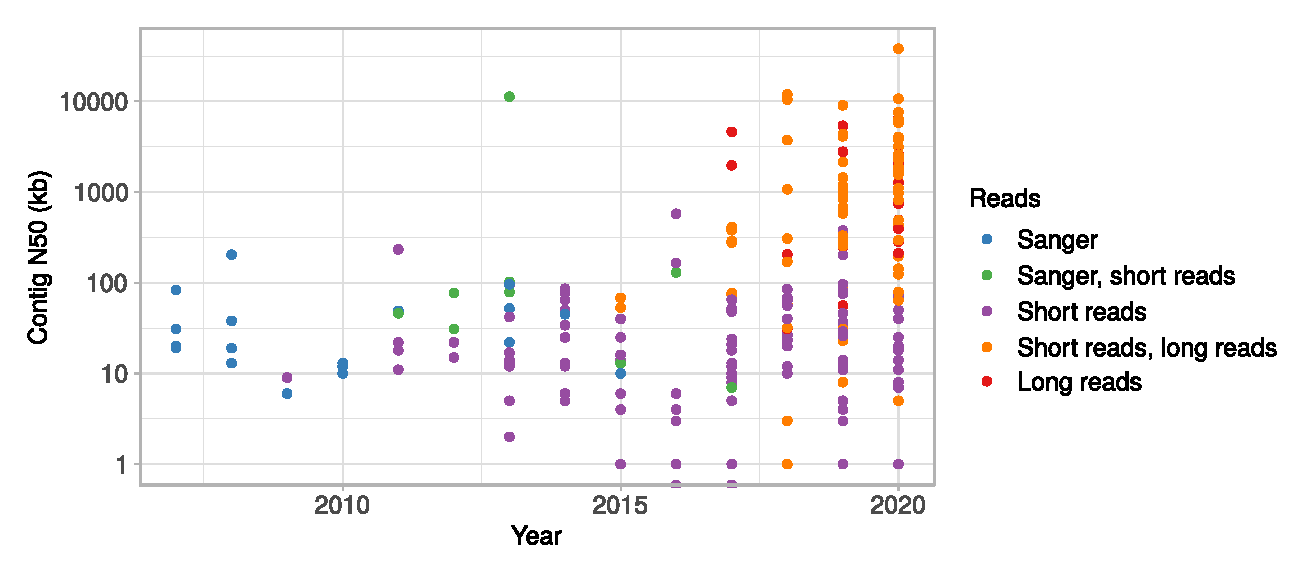
\includegraphics[width=\textwidth]{fig/review_contig_N50_year.eps}
    \caption{Contig N50 of non-vertebrate genome assemblies over time. The N50 represents the contiguity of an assembly and is defined as the length of the largest contig for which 50\% of the assembly size is contained in contigs of equal or greater length.}
    \label{fig:contig_N50_year}
\end{figure}

Third-generation sequencing have brought a whole new range of sequencing data, with the sequencing of long DNA molecules extending up to hundreds of thousands of bases \cite{pollard2018}. The two main players in the field,  Pacific Biosciences (PacBio) and Oxford Nanopore Technologies (Nanopore), use two different kinds of technologies. PacBio developed Single Molecule Real-Time (SMRT) sequencing, where a complementary strand of DNA is produced from a single strand by addition of fluorescently labeled nucleotides. The fluorescent tag is released and the luminescence is interpreted as a base \cite{pacbio_smrt}. The resulting reads have a length around twenty kilobases and a high error rate, an issue recently addressed by the introduction of an extra step called Circular Consensus Sequencing (CCS). In CCS, the DNA polymerase passes multiple times on the same base on a circularized strand to produce High Fidelity (HiFi) reads that can achieve accuracy over 99\% \cite{pacbio_ccs}. \\

Nanopore sequencing uses a membrane with protein pores, through which an electrical current is flowing. DNA strands are pulled through the pores, with each passing nucleotide generating a distinct disruption signature in the current that can be inferred as a specific base \cite{nanopore}. The firm has specifically oriented its strategy toward a "do it yourself" approach, enabling sequencing in any lab and even directly in the field via a small portable device \cite{minion}. Researchers can control how they generate their sequencing data, contribute to protocol development, and develop their own basecalling \cite{basecallers} to increase the yield and improve the quality and length of the reads. Although Nanopore reads still exhibit a high error rate, their length keeps increasing to attain hundreds of kilobases to 1 Megabase (Mb) \cite{Jain2018}. Besides, the error rate has also been decreasing with the release of the new flow cells and the development of more accurate basecallers such as Bonito \cite{bonito}. \\

Long reads are now routinely included in genome assembly projects and have lead to N50 lengths much larger than short-read only assemblies (Figure \ref{fig:contig_N50_year}). A current limitation lies in the amount of DNA required to prepare long-read libraries. Still, long-read sequencing remains inaccessible for certain species: whereas Illumina sequencing can handle small DNA amounts, with a poor quality, long-read protocols require high-molecular weight DNA \cite{dna-extraction}. PacBio and Nanopore sequencing remain difficult when one animal is too small to provide a sufficient amount of DNA, especially when the organism requires extraction protocols that lead to overly fragmented DNA (for example, with coral skeletons). In addition, secondary metabolites associated to DNA molecules, or branched DNA structures, can also disturb the sequencing reaction. \\

\section{Genome assembly}

A variety of programs have been developed to assemble sequencing reads \textit{de novo}, taking advantage of the different sequencing technology while considering their limitations. Genome assembly aims to correctly reconstruct the original chromosome sequences from short or long, and accurate or error-prone fragments. Assemblers are typically based on one of the following paradigms: greedy, Overlap-Layout-Consensus, de Bruijn graphs. \\

\begin{table}
\caption{Sequencing approaches and associated assemblers.}
\centering
\begin{tabular}{|l|l|l|l|l|}
    \hline
    \textbf{Sequencing} & \textbf{Length} & \textbf{Accuracy} & \textbf{Methods} & \textbf{Assemblers}\\
    \hline
    First & 1 kb & High & Sanger & ARACHNE \cite{arachne}, Atlas \cite{atlas}, CAP3 \cite{cap3}, \\
    generation &  &  &  & Celera \cite{celera}, Euler \cite{euler}, JAZZ \cite{jazz},  \\
        &  &  &  & Minimus \cite{minimus}, MIRA \cite{mira}, phrap \cite{phrap}, \\
        &  &  &  & Phusion \cite{phusion}, SUTTA \cite{sutta}, TIGR \cite{tigr} \\
    \hline
    Second & 25-300 bp & High & 454, IonTorrent, & ABySS \cite{abyss,abyss2}, ALLPATHS \cite{allpaths}, \\
    generation &  &  & Solexa, SOLiD & CABOG \cite{cabog}, Edena \cite{edena}, Euler-SR \cite{euler-sr}, \\
        &  &  &  & Gossamer \cite{gossamer}, IDBA \cite{idba}, \\
        &  &  &  & JR-Assembler \cite{jr-assembler}, Meraculous \cite{meraculous}, \\
        &  &  &  & MIRA \cite{mira}, Newbler, NOVOPlasty \cite{novoplasty},  \\ 
        &  &  &  & PCAP \cite{pcap}, PERGA \cite{perga}, Platanus \cite{platanus},  \\
        &  &  &  & QSRA \cite{qsra}, Ray \cite{ray}, Readjoiner \cite{readjoiner}, \\
        &  &  &  & SGA \cite{sga}, SOAPdenovo \cite{soapdenovo}, \\
        &  &  &  & SOAPdenovo2 \cite{soapdenovo2} SPAdes \cite{spades}, \\
        &  &  &  & SSAKE \cite{ssake}, SUTTA \cite{sutta}, Taipan \cite{taipan}, \\
        &  &  &  & VCAKE \cite{vcake}, Velvet \cite{velvet} \\
    \hline
    Third & 10-100.000+ kb & Low & PacBio CLR, & Canu \cite{canu}, FALCON \cite{falcon-unzip}, Flye \cite{flye}, \\
    generation &  &  & Nanopore & HINGE \cite{hinge}, MECAT \cite{mecat}, \\
        &  &  &  & MECAT2 \cite{mecat}, miniasm \cite{miniasm}, \\
        &  &  &  & NECAT \cite{necat},NextDenovo \cite{nextdenovo}, Ra \cite{ra}, \\
        &  &  &  & Raven \cite{raven}, Shasta \cite{shasta}, \\
        &  &  &  & SMARTdenovo \cite{smartdenovo}, wtdbg \cite{wtdbg}, \\
        &  &  &  & wtdbg2 \cite{wtdbg2} \\
        & 20 kb & High & PacBio HiFi & Flye \cite{flye}, HiCanu \cite{hicanu}, hifiasm \cite{hifiasm}, \\ 
        &  &  &  & IPA \cite{IPA}, MIRA \cite{mira}, Peregrine \cite{peregrine}\\
    \hline
\end{tabular}
\label{tab:sequencing}
\end{table}


The assembly problem can be represented as a linear puzzle where the pieces are the reads. Reads match together when they have overlapping sequences. This puzzle could be intuitively solved by iteratively putting overlapping pieces together with the best matching piece: this greedy approach is an efficient heuristic to find the shortest common superstring of the set of reads (i.e., the shortest sequence that includes all the reads as substrings) \cite{greedy}. Greedy algorithms have been implemented for first-generation sequencing reads, for instance in TIGR \cite{tigr}, and were further applied in short-read assemblers like PERGA \cite{perga}, SSAKE \cite{ssake} and VCAKE \cite{vcake}. However, they cannot resolve complex, repetitive genomes: for this reason, greedy assemblers are mostly used nowadays to assemble small organelle genomes such as chloroplasts and mitochondria \cite{novoplasty}. \\

The Overlap-Layout-Consensus (OLC) paradigm was first described in 1979 by Rodger Staden \cite{olc} and is based on an overlap graph (Figure \ref{fig:olc}). The Overlap step consists in finding all the overlaps between all the reads and building a directed graph, where the nodes are the reads and the edges represent the overlaps between them. The Layout step removes redundant edges that can be inferred from other edges. Finally, the Consensus step finds an optimal path in the graph. The OLC paradigm has thrived with the program Celera \cite{celera}, which was used to assemble a human genome from a Sanger shotgun dataset \cite{venter2001}. \\

\begin{figure}
    \centering
    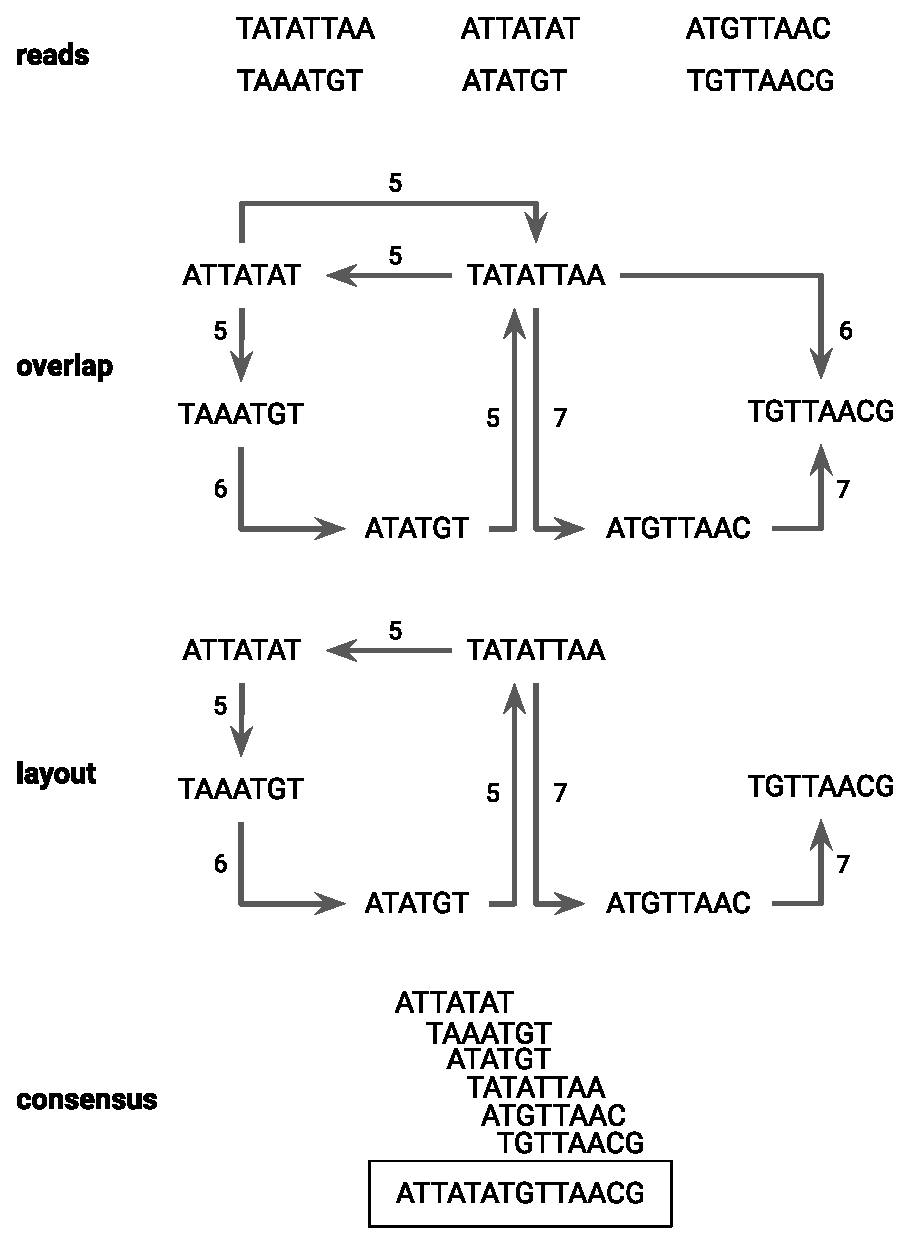
\includegraphics[width=\textwidth]{fig/review_olc.eps}
    \caption{Overview of Overlap Layout Consensus.}
    \label{fig:olc}
\end{figure}

De Bruijn Graphs (DBGs) (Figure \ref{fig:dbg}) are a well studied structure in graph theory, described by Nicolaas Govert de Bruijn in 1946 \cite{dbg} and before him by Camille Flye Sainte-Marie \cite{flyesaintemarie}. DBG-based assemblers require highly accurate reads in which errors are only substitutions, with no indels. They detect all the different sequences of a given \textit{k} length (\textit{k}-mers). Two \textit{k}-mers are connected in the graph when they have an overlap of a \textit{k}-1 length. The approach was first adapted for genome assembly of first-generation sequencing datasets \cite{Compeau2011} and was quickly implemented in multiple popular short-read assemblers, e.g. ABySS \cite{abyss, abyss2}, IDBA \cite{idba}, SOAPdenovo \cite{soapdenovo} and SOAPdenovo2 \cite{soapdenovo2}, SPAdes \cite{spades}, Velvet \cite{velvet}. \\

\begin{figure}
    \centering
    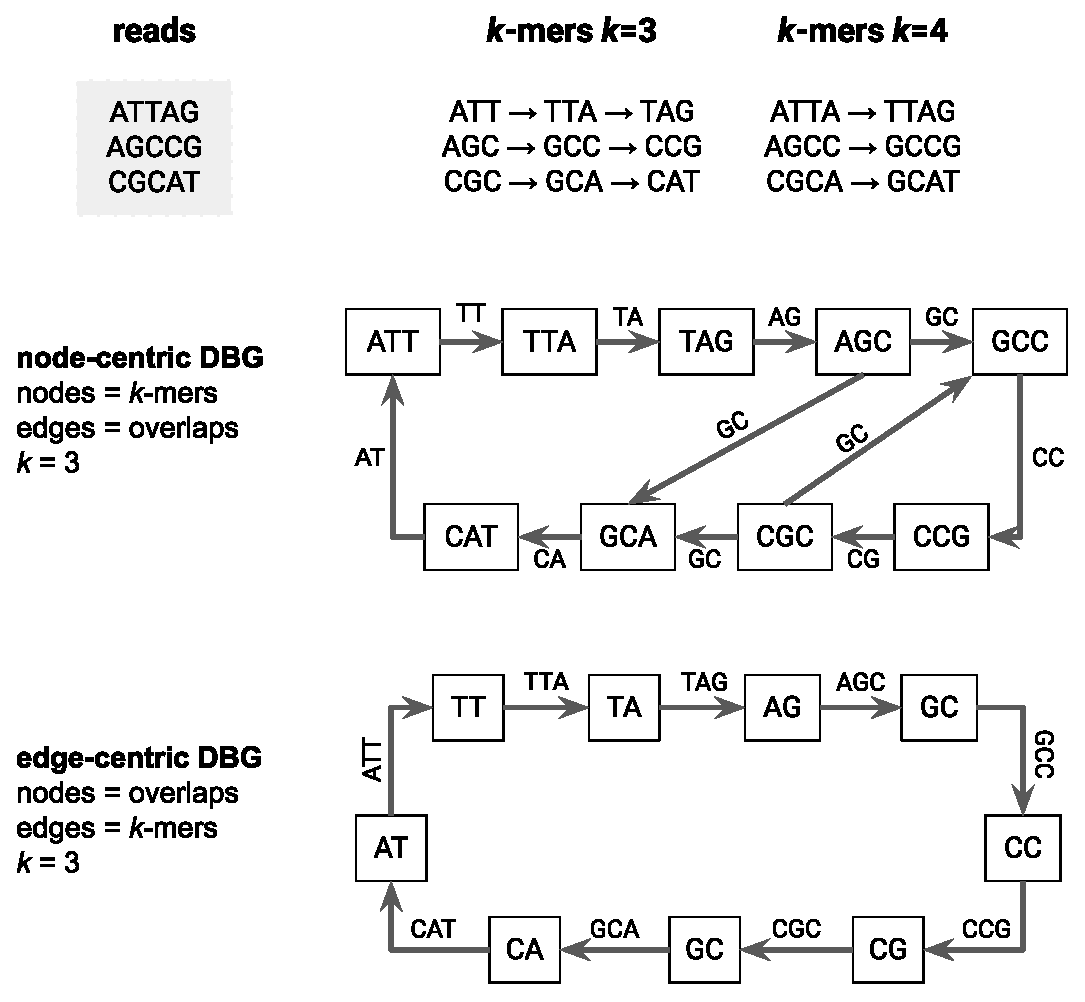
\includegraphics[width=\textwidth]{fig/review_de_bruijn_graph.eps}
    \caption{Overview of de Bruijn graphs.}
    \label{fig:dbg}
\end{figure}


With the advent of third-generation sequencing, OLC assemblers have benefited from a renewed interest whereas DBG-based ones are unsuited for long, low-accuracy reads, containing many erroneous \textit{k}-mers. Many assemblers have implemented OLC to produce \textit{de novo} assemblies from error-prone long-read datasets: Flye \cite{flye}, Ra \cite{ra}, Raven \cite{raven}, Shasta \cite{shasta}, wtdbg2 \cite{wtdbg2}. Now that HiFi reads bring a new type of high accuracy long reads, assemblers have been adapted to better handle these sequences, such as Flye (with adapted parameters), HiCanu \cite{hicanu} and hifiasm \cite{hifiasm}, and we can expect the development of new DBG assemblers adapted for large \textit{k}-mer values \cite{bankevich2020}. \\

From sequencing reads, assemblers build contiguous sequences called contigs. A perfectly assembled genome should have one contig representing each chromosome, but this is rarely achieved for eukaryotes. Assemblers need to find unambiguous paths in the assembly graph to reconstitute the chromosomes, but they often fail to do so due to the genomic structure: size, heterozygosity, repetitive content. Large genomes require a high amount of sequencing data in order to reach a sufficient depth to represent every loci. Genome sizes have a high variability even within phyla (Figure \ref{fig:sizes}). For instance, in the phylum Cnidaria, some myxozoans have a genome size of only some tens of Megabases (Mb) (\textit{Kudoa iwatai}: 22.5 Mb, \textit{Myxobolus squamalis}: 53.1 Mb, \textit{Henneguya salminicola}: 60.0 Mb \cite{henneguya_salminicola}), while the hydrozoan \textit{Hydra oligactis} (1.3 Gb) \cite{hydra_oligactis} has a genome size two orders of magnitude larger. Such differences are also observed for the phyla Annelida, Arthropoda and Mollusca. 
Heterozygous regions constitute a major cause for breaks in assemblies of non-model animal genomes, as they generally have higher levels of heterozygosity than model species \cite{Leffler2012a}. Most assemblers try to build a haploid representation of all genomes, even for multiploid (i.e. diploid or polyploid) genomes. To this end, heterozygous regions are collapsed in order to keep a single sequence for every region in the genome. In an assembly graph, these heterozygous regions will manifest themselves as bubbles, where one contig (a homozygous region) can be connected to several other contigs (the alternative haplotypes of a heterozygous region). When the assembler is unable to select one path, the homozygous region is not joined with any of the haplotypes, leading to a break in the assembly. 

\begin{figure}
    \centering
    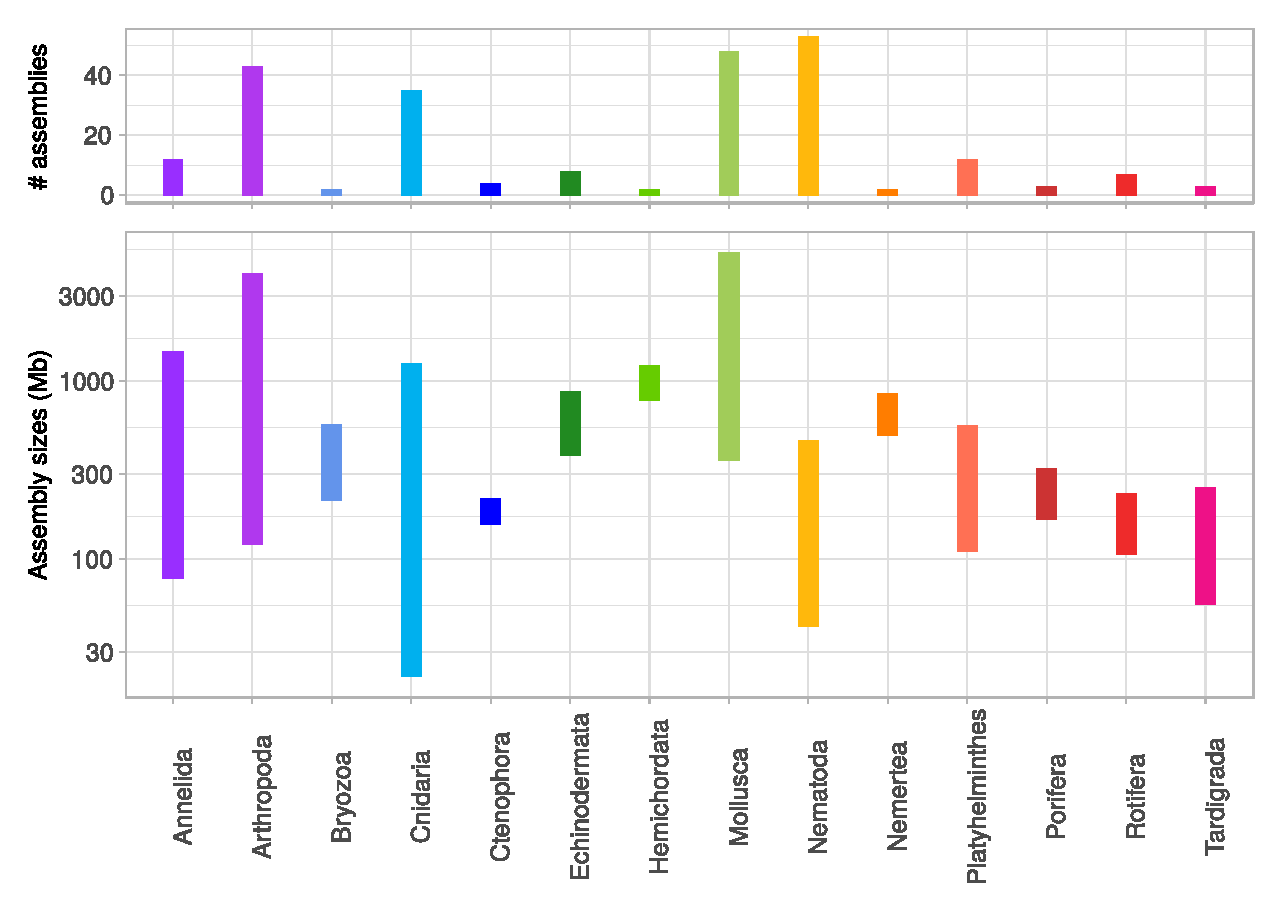
\includegraphics[width=\textwidth]{fig/review_assembly_sizes.eps}
    \caption{Assembly sizes. The top graph shows the number of assemblies included for each phylum and the lower part the corresponding assembly-size ranges.}
    \label{fig:sizes}
\end{figure}

\section{Assembly pre and post-processing}

\begin{table}
\caption{Assembly pre and post-processing tools for haploid assemblies.}
\begin{tabular}{|l|l|l|}
\hline
\textbf{Step} & \textbf{Sequencing data} &\textbf{Tools} \\
\hline
Reads filtering & Long reads & Filtlong \cite{filtlong} \\
\hline
Long reads & Short reads & CoLoRMAP \cite{colormap}, Hercules \cite{hercules}, Jabba \cite{jabba}, LoRDEC \cite{lordec}, \\
error correction &  & LoRMA \cite{lorma}, proovread \cite{proovread} \\
    \cline{2-3}
    & Long reads & Canu \cite{canu}, CONSENT \cite{consent}, Daccord \cite{daccord}, FLAS \cite{flas}, \\
    &  & NextDenovo \cite{nextdenovo}, MECAT \cite{mecat}, MECAT2 \cite{mecat} \\
\hline
Polishing & Short reads & ntEdit \cite{ntedit}, Pilon \cite{pilon}, POLCA \cite{polca} \\
    \cline{2-3}
    & Short \& long reads & Apollo \cite{apollo}, HyPo \cite{hypo}, Racon \cite{racon} \\
    \cline{2-3}
    & Long reads & Arrow \cite{quiver_arrow}, CONSENT \cite{consent}, Medaka \cite{medaka}, NextPolish \cite{nextpolish}, \\
    &  & Nanopolish \cite{nanopolish}, Quiver \cite{quiver_arrow} \\
\hline
Haplotigs purging & Long reads & HaploMerger2 \cite{haplomerger2}, purge\_dups \cite{purge_dups}, Purge Haplotigs \cite{purge_haplotigs} \\
\hline
Scaffolding & Short reads & Bambus \cite{bambus}, BATISCAF \cite{batiscaf}, BESST \cite{besst}, BOSS \cite{boss}, \\
    & Mate pairs & GRASS \cite{grass}, MIP \cite{mip}, Opera \cite{opera}, ScaffMatch \cite{scaffmatch}, \\
    &  & ScaffoldScaffolder \cite{scaffoldscaffolder}, SCARPA \cite{scarpa}, SCOP \cite{scop}, SLIQ \cite{sliq}, \\
    &  & SOPRA \cite{sopra}, SSPACE \cite{sspace}, WiseScaffolder \cite{wisescaffolder} \\
    \cline{2-3}
    & Long reads & LINKS \cite{links}, LRScaf \cite{lrscaf}, npScarf \cite{npScarf}, PBJelly \cite{pbjelly}, \\
    &  & RAILS \cite{rails}, SLR \cite{slr}, SMIS \cite{smis}, SMSC \cite{smsc}, \\
    &  & SSPACE-LongRead \cite{sspace-longread} \\
    \cline{2-3}
    & Genetic maps & ALLMAPS \cite{allmaps} \\
    \cline{2-3}
    & Optical maps & AGORA \cite{agora}, BiSCoT \cite{biscot}, OMGS \cite{omgs}, SewingMachine \cite{sewingmachine}, \\
    &  & SOMA \cite{soma} \\
    \cline{2-3}
    & Linked reads & ARBitR \cite{arbitr}, Architect \cite{architect}, ARCS \cite{arcs}, ARKS \cite{arks}, \\ 
    &  & fragScaff \cite{fragscaff}, Scaff10X \cite{scaff10X} \\
    \cline{2-3}
    & 3C/Hi-C & 3D-DNA \cite{3d-dna}, dnaTri \cite{dnatri}, GRAAL \cite{graal}, HiCAssembler \cite{hicassembler} \\
    &  & instaGRAAL \cite{instagraal}, Lachesis \cite{lachesis}, SALSA \cite{salsa}, SALSA2 \cite{salsa2} \\
\hline
Gap filling & Short reads & GapFiller \cite{gapfiller}, GAPPadder \cite{gappadder}, Sealer \cite{sealer} \\
    \cline{2-3}
    & Long reads & Cobbler \cite{rails}, FGAP \cite{fgap}, GMcloser \cite{gmcloser}, LR\_Gapcloser \cite{lrgapcloser}, \\
    &  & PBJelly \cite{pbjelly}, PGcloser \cite{pgcloser}, TGS-GapCloser \cite{tgsgapcloser} \\
\hline
\end{tabular}
\label{tab:scaffolding}
\end{table}

As obtaining high-quality chromosome-level contigs still remains challenging, many upstream and downstream tools have been developed in conjunction with assemblers (Table \ref{tab:scaffolding}). Researchers can test numerous combinations of these tools to devise the pipeline that will yield the best assembly. \\

Long reads have the advantage over short reads that they result in more contiguous assemblies. Nevertheless, assemblies of PacBio Continuous Long Reads (CLR) or Nanopore reads can have remaining errors due to their low accuracy; while errors in PacBio CLR are random and are compensated with a high coverage, Nanopore reads have systematic errors in homopolymeric regions. Assemblies of error-prone long reads often necessitate additional processes to increase the quality. There are two possible strategies: correct the long reads prior to assembly, and polish the contigs after assembly. Correcting long reads can be done using only the long reads or by adding high-accuracy short reads. Many tools have been developed for both scenarii and have been thoroughly reviewed on multiple datasets \cite{correction_benchmark}. When tested on \textit{C. elegans} Nanopore reads, the error rate decreased from 28.93\% to less than 1\% (using Canu \cite{canu}, CONSENT \cite{consent}, FLAS \cite{flas}, Jabba \cite{jabba}, LORMA \cite{lorma} or MECAT \cite{mecat}). Some assemblers include a self-correction step in their pipeline, namely Canu \cite{canu}, MECAT \cite{mecat}, NextDenovo \cite{nextdenovo}. Assembling corrected reads is expected to yield contigs with higher quality and contiguity. Alternatively, or additionally, the contigs can be polished to reduce errors, using long reads and/or short reads. Polishing can be a more computationally efficient strategy: the reads are mapped solely to the draft assembly, while correction is usually based on an all-versus-all read mapping. \\

Assemblers are generally tested on model-organism datasets, and are ill-suited for non-model genomes with variable levels of heterozygosity. They often fail to collapse highly divergent haplotypes, causing artefactually duplicated regions that hinder subsequent analyses \cite{ko2021widespread}. Some long-read assemblers, Ra and wtdbg2, have been identified as less prone to retain uncollapsed haplotypes \cite{guiglielmoni2020}. Contigs can also be post-processed to remove these duplications with dedicated tools such as HaploMerger2 \cite{haplomerger2}, purge\_dups \cite{purge_dups} and Purge Haplotigs \cite{purge_haplotigs}. HaploMerger2 detects uncollapsed haplotypes based on sequence similarities, while purge\_dups and Purge Haplotigs also rely on coverage depth. \\

To improve the contiguity of an assembly, contigs can be grouped, ordered and oriented into scaffolds. These scaffolds may contain gaps, when the sequence that should connect two contigs cannot be retrieved, and these gaps are represented as a sequence of Ns. Several sequencing techniques have been used to reach scaffold assemblies: mate pairs, long reads, genetic maps, optical mapping, linked reads, and proximity ligation \cite{ghurye2019modern}. Mate pairs are short reads with a large insert size (more than several kb), and have been widely used in next-generation assemblies. Among the 237 assemblies we surveyed, 78 included a mate-pair scaffolding step (Figure \ref{fig:hic}). Both genetic maps \cite{genetic_maps} and optical maps \cite{optical_maps} provide information on the linkage and relative position of a set of markers, spread over the genome, thus they can be used to anchor contigs. Genetic maps were used for the genome assemblies of the flatworm \textit{Schistosoma mansoni} \cite{schistosoma_mansoni2} and the copepod \textit{Tigriopus japonicus} \cite{tigriopus_japonicus}. Although existing genetic maps provide precious resources, building one is particularly difficult as it requires breeding \cite{genetic_maps}, making it hardly accessible for wild species, and impossible for asexual species. Markers of optical maps are motifs in the sequence that are labeled and detected by a fluorescent signal. Companies such as Bionano or Nabsys propose this service to scaffold assemblies \cite{optical_scaffolding}, and this method was included in some non-vertebrate genome projects: several nematodes including \textit{Onchocerca volvulus} \cite{onchocerca_volvulus}, \textit{Ascaris suum} and \textit{Parascaris univalens} \cite{ascaris_suum2}, the tapeworms \textit{Echinococcus multilocularis} \cite{echinococcus_multilocularis} and \textit{Hymenolepis microstoma} \cite{hymenolepis_microstoma2}, and the chiton \textit{Acanthopleura granulata} \cite{acanthopleura_granulata}. \\

\begin{figure}
    \centering
    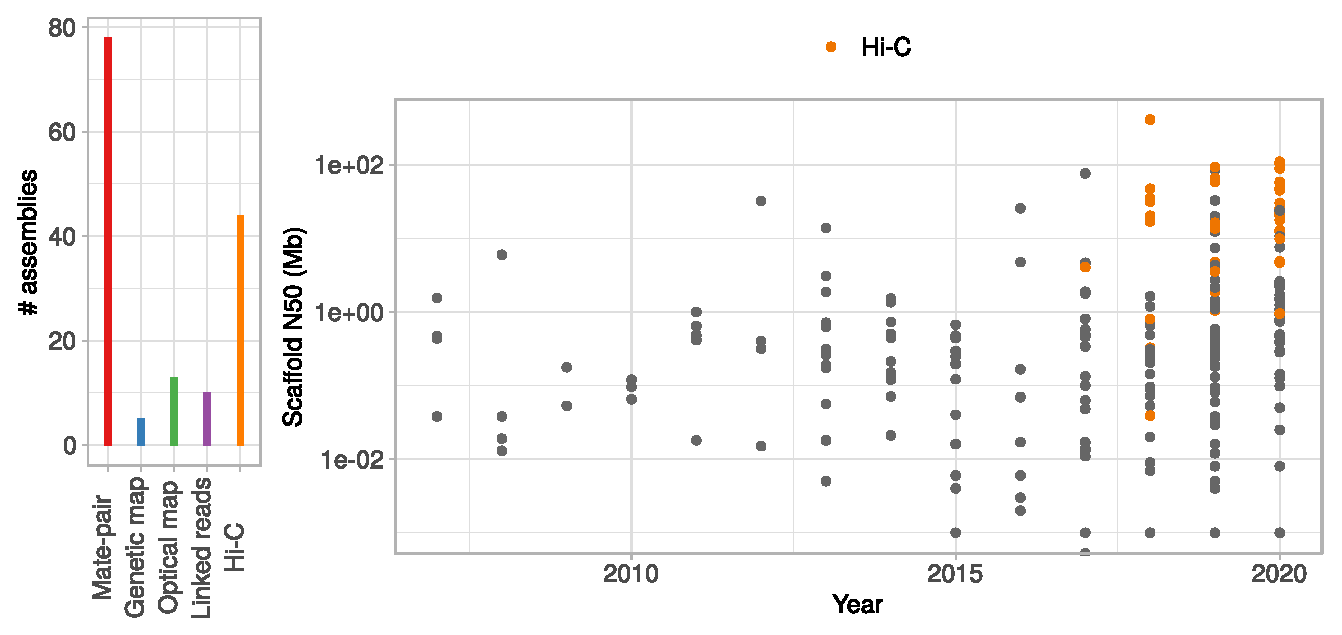
\includegraphics[width=\textwidth]{fig/review_scaffolding.eps}
    \caption{Assemblies scaffolding. Left: number of assemblies that included each scaffolding method. Right: scaffold N50 of non-vertebrate genome assemblies over time. The assemblies that included a Hi-C scaffolding step are highlighted in red; they form a cluster with a scaffold N50 over 1 Mb.}
    \label{fig:hic}
\end{figure}

Linked reads and proximity ligation are based on short-read sequencing, preceded by a specific library preparation. For linked reads, also called cloud reads, long fragments of DNA are barcoded and then sequenced. The company 10X Genomics was a leader of this technology, but they chose to discontinue its commercialization in June 2020. Linked reads have been used to scaffold the genomes of the coral \textit{Acropora millepora} \cite{acropora_millepora2} and the bee \textit{Lasioglossum albipes} \cite{lasioglossum_albipes}. As linked reads are also shotgun Illumina reads, these reads are sometimes used for assembly (using Architect \cite{architect} or Supernova \cite{supernova}) or polishing, as was done for the mosquito \textit{Anopheles funestus} \cite{anopheles_funestus}.
On the other hand, proximity ligation techniques, based on capture of chromosome conformation \cite{Dekker2002}, were not originally developed with genome sequencing applications in mind. Instead, they aimed at investigating the interplay between chromosome 3D organization and DNA processes \cite{dekker2013exploring}. A popular genomic derivative of 3C, Hi-C \cite{Lieberman-Aiden2009} documents the average conformation of the genomes of a population of cells. Briefly, the approach consists in freezing the chromosome folding of each individual cell using chemical fixation by formaldehyde, which generates bonds between proteins and proteins, and proteins and DNA. Then, the genome is cut into fragments using a restriction enzymes, that are then ligated in dilute conditions. As a consequence, fragments that were trapped by the crosslinking step together are more prone to be ligated with each other, rather than with a fragment belonging to a different crosslinked complex. This results in chimeric fragments with respect to the original genome agencement, reflective of their 3D contacts \textit{in vivo}. The relative proportions of ligation events between all restriction fragments of a genome can then be quantified, in theory, through high-throughput sequencing. On average, and because of the polymer nature and physical properties of DNA, the frequency of contacts between a pair of loci reflects either their 1D \textit{cis} disposition along a chromosome, or their \textit{trans} disposition on two independent chromosomes \cite{flot2015contact, oddes2018}. Hi-C scaffolders have been developed following these principles: some follow a graph approach and use Hi-C links to join contigs (3D-DNA \cite{3d-dna}, SALSA2 \cite{salsa2}), whereas others exploit Markov Chain Monte Carlo (MCMC) sampling and Bayesian statistics to reorganize DNA segments into the scaffolds most likely to explain the observed interaction frequencies (GRAAL \cite{graal} and its later improved version instaGRAAL \cite{instagraal}). The Hi-C protocol itself is becoming more and more accessible as commercial kits are now available (e.g. Arima Hi-C, Phase Genomics, or Dovetails Genomics). Besides, Dovetails Genomics uses both regular Hi-C and its own protocol for \textit{in vitro} proximity ligation, dubbed CHICAGO. Hi-C scaffolding proved efficient at bringing highly fragmented draft assemblies to chromosome-level scaffolds (Figure \ref{fig:hic}), and is now included in many genome projects for all sorts of non-vertebrates: the arthropods \textit{Varroa destructor} \cite{varroa_destructor} and \textit{Carcinoscorpius rotundicauda} \cite{carcinoscorpius_rotundicauda2}, the cnidarians \textit{Xenia sp.} \cite{xenia_sp} and \textit{Rhopilema esculentum} \cite{rhopilema_esculentum}, the echinoderms \textit{Lytechinus variegatus} \cite{lytechinus_variegatus} and \textit{Pisaster ochraceus} \cite{pisaster_ochraceus}, the molluscs \cite{scapharca_broughtonii} and \textit{Chrysomallon squamiferum} \cite{chrysomallon_squamiferum}, the nematods \textit{Caenorhabditis remanei} \cite{caenorhabditis_remanei2} and \textit{Heterodera glycines} \cite{heterodera_glycines2}, the platyhelminthe \textit{Schistosoma haemotabium} \cite{schistosoma_haematobium}, the poriferan \textit{Ephydatia muelleri} \cite{ephydatia_mulleri}, the rotifer \textit{Adineta vaga} \cite{adineta_vaga2}, the xenacoelomorph \textit{Hofstenia miamia} \cite{hofstenia_miamia}, and more. A compelling advantage of Hi-C scaffolding over other scaffolding methods is its ability to discriminate different organisms in a draft assembly: DNA from different organisms belong to distinct nuclei, thus they have no 3D interactions. This feature is especially useful for non-vertebrates with symbionts, that can hardly be eliminated from the host prior to sequencing, and are often targets for genome assembly as well.

\section{Assemblies evaluation}

A critical step in genome assembly is to estimate the quality of draft assemblies, and choose the best one for subsequent analysis. The first metric to assess is the assembly size and its adequacy with an estimated genome size. The size can be estimated experimentally with flow cytometry or Feulgen densitometry \cite{mulligan2014}, but these methods require a reference species for which the genome size is already well known, exposing them to errors induced by the reference genome size. Reference-free genome size estimation tools are typically \textit{k}-mer based approaches and use high-accuracy reads (e.g. Illumina, HiFi). These tools, such as BBtools \cite{bbtools}, GenomeScope \cite{genomescope} and KAT \cite{kat_evaluation}, build a \textit{k}-mer spectrum representing the number of \textit{k}-mers with a certain frequency of occurence. When the sequencing depth is sufficient, the \textit{k}-mer spectrum should display one or more peaks depending on the ploidy. For a haploid organism, there should be only one peak, whereas a diploid organism should have two peaks. The plot may also show a peak of \textit{k}-mers with a frequency of occurence close to zero, corresponding to erroneous \textit{k}-mers. Another recent tool called MGSE \cite{mgse} estimates genome size based on reads mapping to a highly continuous assembly of the same genome; this method can be used as a post-hoc analysis. \\

N50 is a popular metric that reflects the contiguity of an assembly: it is defined as the length of the largest contig for which 50\% of the assembly size is contained in contigs of equal or greater length. Some tools provide in addition the N75, N90, N99, computed in a similar fashion. The NG50 is a variant of N50 that refers to an estimated genome size instead of the assembly size. The target assembly can further be mapped against a reference assembly to detect misassemblies and break them: the N50 and NG50 of the resulting fragments are called NA50 and NGA50. All these metrics can be computed using QUAST \cite{quast}. For genome assemblies of non-model non-vertebrates, reference assemblies are seldom available, or they have a poor quality or contiguity that the new assembly aspires to improve. Therefore we will focus on reference-free evaluation methods. We present in Table \ref{tab:assembly_stats} and Figure \ref{fig:evaluation} an example of assembly evaluation for the recently published snail \textit{Achatina fulica} \cite{achatina_fulica} and coral \textit{Xenia sp.} \cite{xenia_sp}. \\

\begin{table}
\centering
\caption{Assembly evaluation of \textit{Achatina fulica} and \textit{Xenia sp.}.}
\begin{tabular}{|l|l|c|c|}
\hline
                &  & \textit{Achatina fulica} & \textit{Xenia sp.} \\
\hline
Basic statistics & Assembly size & 1.86 Gb & 222.7 Mb \\
                & N50 & 59.6 Mb & 14.8 Mb \\
                & N90 & 44.1 Mb & 6.9 Mb \\
                & Largest scaffold & 116.6 Mb & 22.5 Mb \\
                & Number of scaffolds & 1500 & 168 \\
                & Number of scaffolds larger than 1 Mb & 32 & 17 \\
                & N count & 3,600,500 & 194,000 \\
\hline
BUSCO completeness & Complete and single-copy BUSCOs & 84.4\% & 86.0\% \\
                & Complete and duplicated BUSCOs & 3.6\% & 2.2\% \\
                & Fragmented BUSCOs & 3.5\% & 3.5\% \\
                & Missing BUSCOs & 8.5\% & 8.3\% \\
\hline
Reads mapping & Short reads & 96.2\% & 87.8\% \\
                & Long reads & 81.62\% & 99.5\% \\
                & Hi-C & 70.2\% & 65.7\% \\
\hline
\end{tabular}
\label{tab:assembly_stats}
\end{table}

\begin{figure}
    \centering
    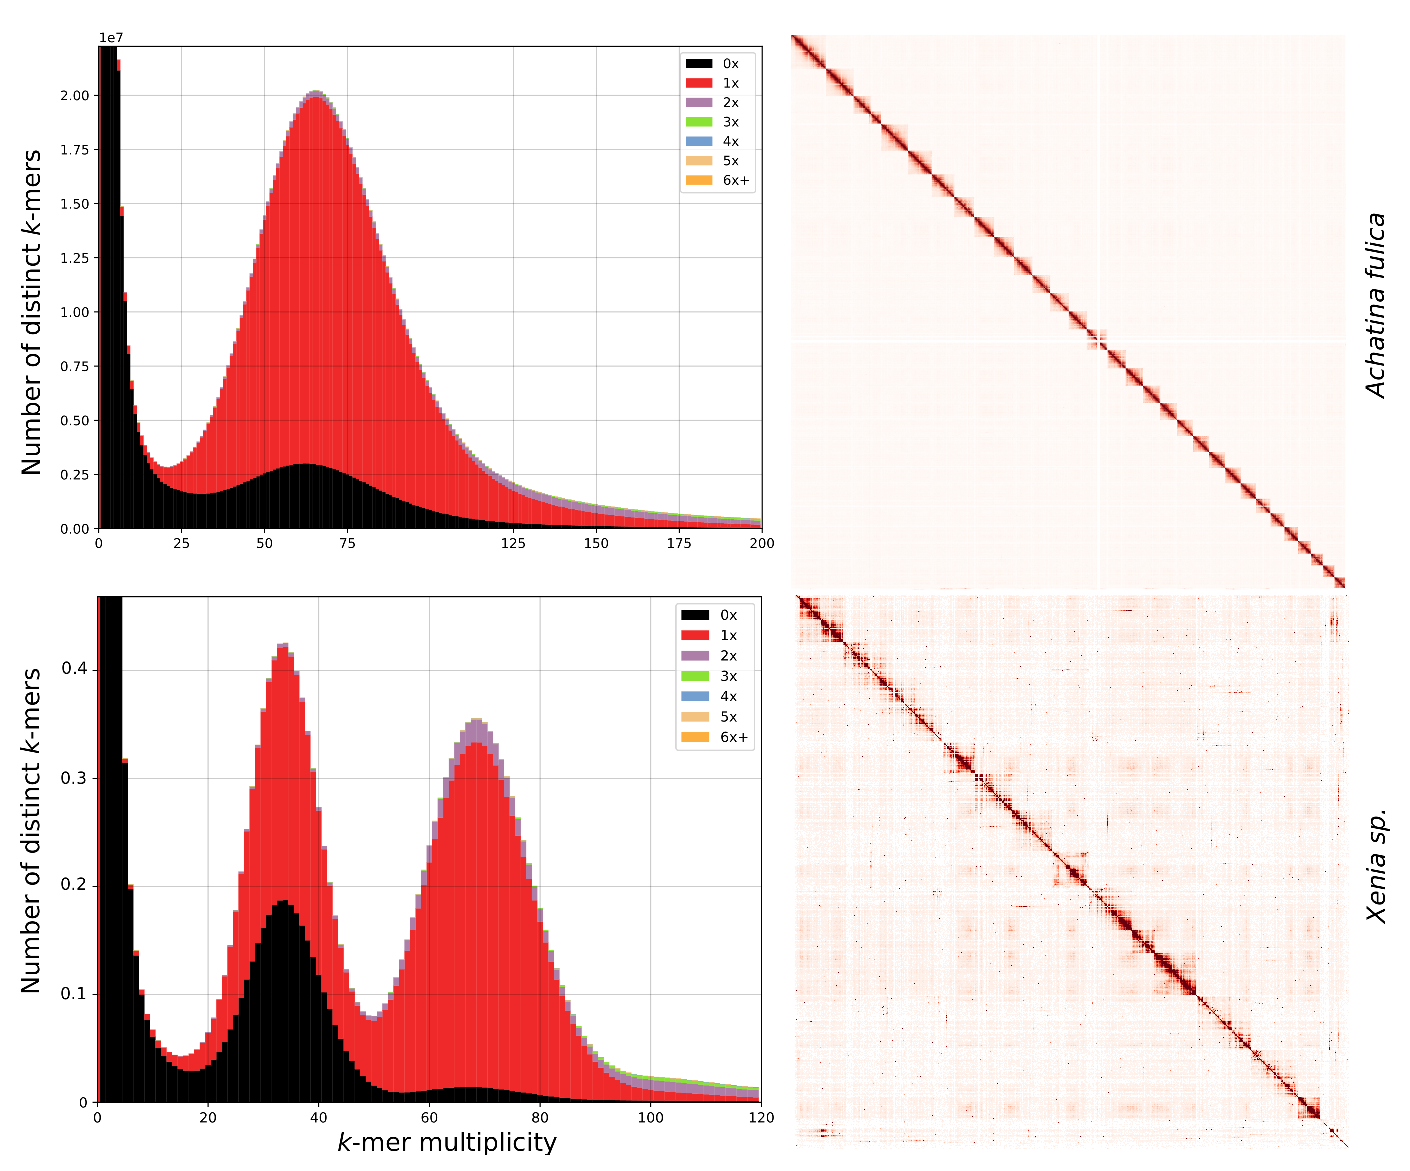
\includegraphics[width=\textwidth]{fig/review_assembly_evaluation.eps}
    \caption{Assembly evaluation of \textit{Achatina fulica} and \textit{Xenia sp.}. Left: KAT comparison of the \textit{k}-mers in the Illumina datasets v. the assembly. Right: Hi-C contact maps, with a binning of 300 for \textit{Achatina fulica}, 30 for \textit{Xenia sp.}.}
    \label{fig:evaluation}
\end{figure}

Another feature to optimize is the completeness of the genome, usually based on orthologs or \textit{k}-mers. BUSCO \cite{busco_evaluation} searches for orthologs in a user-provided lineage; the current Metazoa lineage (designated as Metazoa odb10) contains 954 features. Assemblies are evaluated based on the proportion of orthologs to these 954 genes that can be retrieved into them; yet, some features are systematically missing in some genomes as they are absent from these species. More specific lineages are available for arthropods, insects, vertebrates, mammals, as many assemblies are available for these groups, but other metazoan phyla suffer from their lack of resources. Consequently, BUSCO is most powerful when comparing several draft assemblies for one genome. BUSCO scores provide information on complete single-copy and duplicated features, and the latter can be used to detect improperly duplicated regions in a haploid assembly. However, BUSCO scores are limited to genomic regions and cannot report for non-coding ones. \textit{k}-mer completeness scores do not present such limitations: KAT assesses the completeness of a whole assembly based on its representation of \textit{k}-mers from a high accuracy sequencing dataset. The \textit{k}-mer spectrum should display one or several peaks depending on the ploidy of the genome: one peak for a haploid genome; two peaks for a diploid genome, the first depicting heterozygous \textit{k}-mers, and the second for homozygous \textit{k}-mers. Depending on the ploidy of the genome, every \textit{k}-mers should be represented in the assembly as many times as they actually are in the genome. Both \textit{Achatina fulica} and \textit{Xenia sp.} have high BUSCO scores (against the lineage Metazoa odb10), yet slightly below 90\%, and they have few duplicated BUSCO features. The \textit{k}-mer spectrum of \textit{Achatina fulica} only shows one peak around 70X (Figure \ref{fig:evaluation}, top left). These \textit{k}-mers are expected to be represented exactly once, which is the case for the majority; there are almost no \textit{k}-mers that appear twice in the assembly (in purple), but there is a noteworthy amount of missing \textit{k}-mers (in black). For \textit{Xenia sp.}, the \textit{k}-mer spectrum has two peaks with a \textit{k}-mer multiplicity around 35X and 70X (Figure \ref{fig:evaluation}, bottem left). The first peak, representing heterozygous \textit{k}-mers, shows that a portion is represented once in the assembly, while the rest is missing, as expected in a collapsed assembly. The second peak, for homozygous \textit{k}-mers has a majority of \textit{k}-mers represented once, and some \textit{k}-mers either absent or duplicated. These assembly seems overall properly collapsed and complete. \\

When Hi-C data are available, contact maps, i.e. the representation of the paired-end reads from the Hi-C library aligned on the resulting scaffold, procure another evaluation asset to search for misassemblies. The contact map is expected to show heightened frequencies for each chromosome, in a chromosome-level assembly, and these interaction frequencies should decrease with increased distances separating loci on the sequence, based on the distance law. For \textit{Achatina fulica}, 30 chromosome-level scaffolds (out of 31) display relatively consistent and regular contact patterns, representing well individualized entities in the contact map (Figure \ref{fig:evaluation}, top right).By contrast, the contact map of \textit{Xenia sp.} does not display such patterns, with multiple \textit{trans} contacts appearing between the scaffolds and most likely corresponding to scaffolding errors. \\

\section{Phasing assemblies}

As collapsing multiploid genomes can be difficult for highly divergent regions and frequently causes breaks in the assembly, an intuitive solution would be to phase genomes to retrieve all haplotypes. Phased assemblies represent a whole different challenge as they necessitate to correctly associate alleles, i.e. different versions of a heterozygous region \cite{unzipping}. A first approach, called trio-binning, is to assemble one individual using sequencing data from the individual itself and its parents \cite{triocanu}; yet this method is only adapted when the parents can be identified, and is inapplicable on asexual species. Some tools are able to reconstruct haplotypes from collapsed assemblies using long reads, namely HapCUT2 \cite{hapcut2} and WhatsHap \cite{whatshap}. But alternative haplotypes may encompass large regions in highly heterozygous regions and can be excessively intricate to represent accurately, for example in hemiploid genomes, when one region is present in one haplotype and not in others. Ideally, genomes should be uncollapsed, as can be done with Bwise \cite{bwise} and Platanus-Allee \cite{platanus-allee} using short reads and FALCON-Unzip \cite{falcon-unzip} using PacBio (CLR or HiFi) reads. FALCON-Unzip uses the output from the FALCON assembler, that includes both a haploid assembly and alternative haplotigs for heterozygous regions, to associate haplotypes based on long reads. Phased assemblies of low-accuracy long reads are limited, as small heterozygous regions were confused with errors; this led to haplotypes being erroneously collapsed. HiFi reads have made a disruption in the fields of genomics: they are especially well-suited for phased assemblies thanks to their length and low error rate, and they have already been used to produce phased assemblies of a human \cite{phased_human} and the potato \textit{Solanum tuberosum} \cite{potato}. Nevertheless, sequencing HiFi reads can remain inaccessible for non-model organisms as pure DNA is necessary. Many organisms have already been assembled using low-accuracy longs reads and high-accuracy short reads, thus an alternative is to correct long reads with short reads using a tool that conserves haplotypes such as Ratatosk \cite{ratatosk}. Phased long-read assemblies can be further polished with adequate programs (e.g. Hapo-G \cite{hapog}). As Hi-C has already demonstrated its efficiency to scaffold haploid assemblies, the principles were further exploited in ALLHiC \cite{allhic} and FALCON-Phase \cite{falcon-phase} to phase assemblies while increasing their contiguity: as alleles from one haplotype belong to one chromosome, these alleles have higher Hi-C interaction frequencies together than with alleles from alternative haplotypes. A new approach was proposed recently in the tool GraphUnzip \cite{graphunzip}: this program starts from an uncollapsed assembly graph, rather than a linear sequence, and attempts to phase bubbles using long-range information from long reads and Hi-C. 

\section{Outline of the thesis}

This first chapter introduced the principles of DNA sequencing, genome assembly, and the difficulties specific to non-vertebrate animals. This thesis is divided into two main sections: Chapters 2, 3 and 4 describe methodologies and tools for genome assembly, whereas Chapters 5, 6 and 7 present the application of these methods to genome projects. \\
Chapter 1 evaluates the performances of seven long-read assemblers, and more specifically their behavior on non-model genomes with variable levels of heterozygosity, based on the example of the rotifer \textit{Adineta vaga}. The end goal of this study is to produce high-quality collapsed contigs from multiploid genomes. In Chapter 2, the strategy is the opposite, as the aim is to obtain uncollapsed, phased assemblies. This part presents the tool GraphUnzip, which takes advantage of assembly graphs, long reads and Hi-C reads to yield phased gap-less supercontigs with a high contiguity. Chapter 3 takes contigs to scaffolds with the Hi-C scaffolder instaGRAAL, a new version of GRAAL. Chapter 4, 5 and 6 describe the genome assemblies of \textit{Adineta vaga}, \textit{Astrangia poculata} and \textit{Flaccisagitta enflata}, using the strategies identified in Chapter 2 for long-read assembly, and instaGRAAL for Hi-C scaffolding.  \\

% write your paper in here
\newenvironment{suppsection}{
\newcommand{\beginsupplement}{%
        \setcounter{table}{0}
        \renewcommand{\thetable}{S\arabic{table}}%
        \setcounter{figure}{0}
        \renewcommand{\thefigure}{S\arabic{figure}}%
     }
}

\chapter{Benchmark of long-read assemblers on the genome of the bdelloid rotifer \textit{Adineta vaga}}

Long reads have made highly contiguous assemblies accessible for all genomes, but most long-read assemblers aim to produce a haploid assembly, regardless of the actual degree of ploidy (haploid, diploid or polyploid) of the genome being assembled. To obtain haploid assemblies from diploid or polyploid genomes, homologous chromosomes need to be collapsed into a single sequence. This process is straightforward for homozygous regions, but more challenging for heterozygous regions as the assembler needs to find a consensus between haplotypes or select one to represent the region. Collapsing haplotypes is especially challenging for non-model diploid or polyploid genomes, as they often display variable levels of heterozygosity across their genomes. \\

I designed a benchmark of seven long-read assemblers, namely Canu \cite{canu}, Flye \cite{flye}, NextDenovo \cite{nextdenovo}, Ra \cite{ra}, Raven \cite{raven}, Shasta \cite{shasta} and wtdbg2 \cite{wtdbg2}. I tested these assemblers on the genome of a non-model diploid organism, \textit{Adineta vaga}, for which high-coverage sequencing datasets of both PacBio and Nanopore low-accuracy long reads were available. I investigated the improvement of haplotype-collapsing when combining these assemblers with pre-assembly read filtering and post-assembly haplotig purging. I defined a thorough evaluation strategy to identify the best haploid assemblies, based on assembly size, contiguity, completeness, and a new metric of haploidy that was implemented in the tool HapPy. I also evaluated the impact of sequencing depth on haplotype collapsing and overall assembly quality, and found that most assemblers were optimized for a sequencing depth of 40X. A higher sequencing depth would not necessarily improve the assemblies but would rather lead to more uncollapsed haplotypes. \\

I initiated this benchmark to evaluate how long-read assemblers behaved on a small non-model eukaryote genome, and applied these strategies in several assembly projects for larger genomes, including \textit{Astrangia poculata} and \textit{Flaccisagitta enflata}. \\

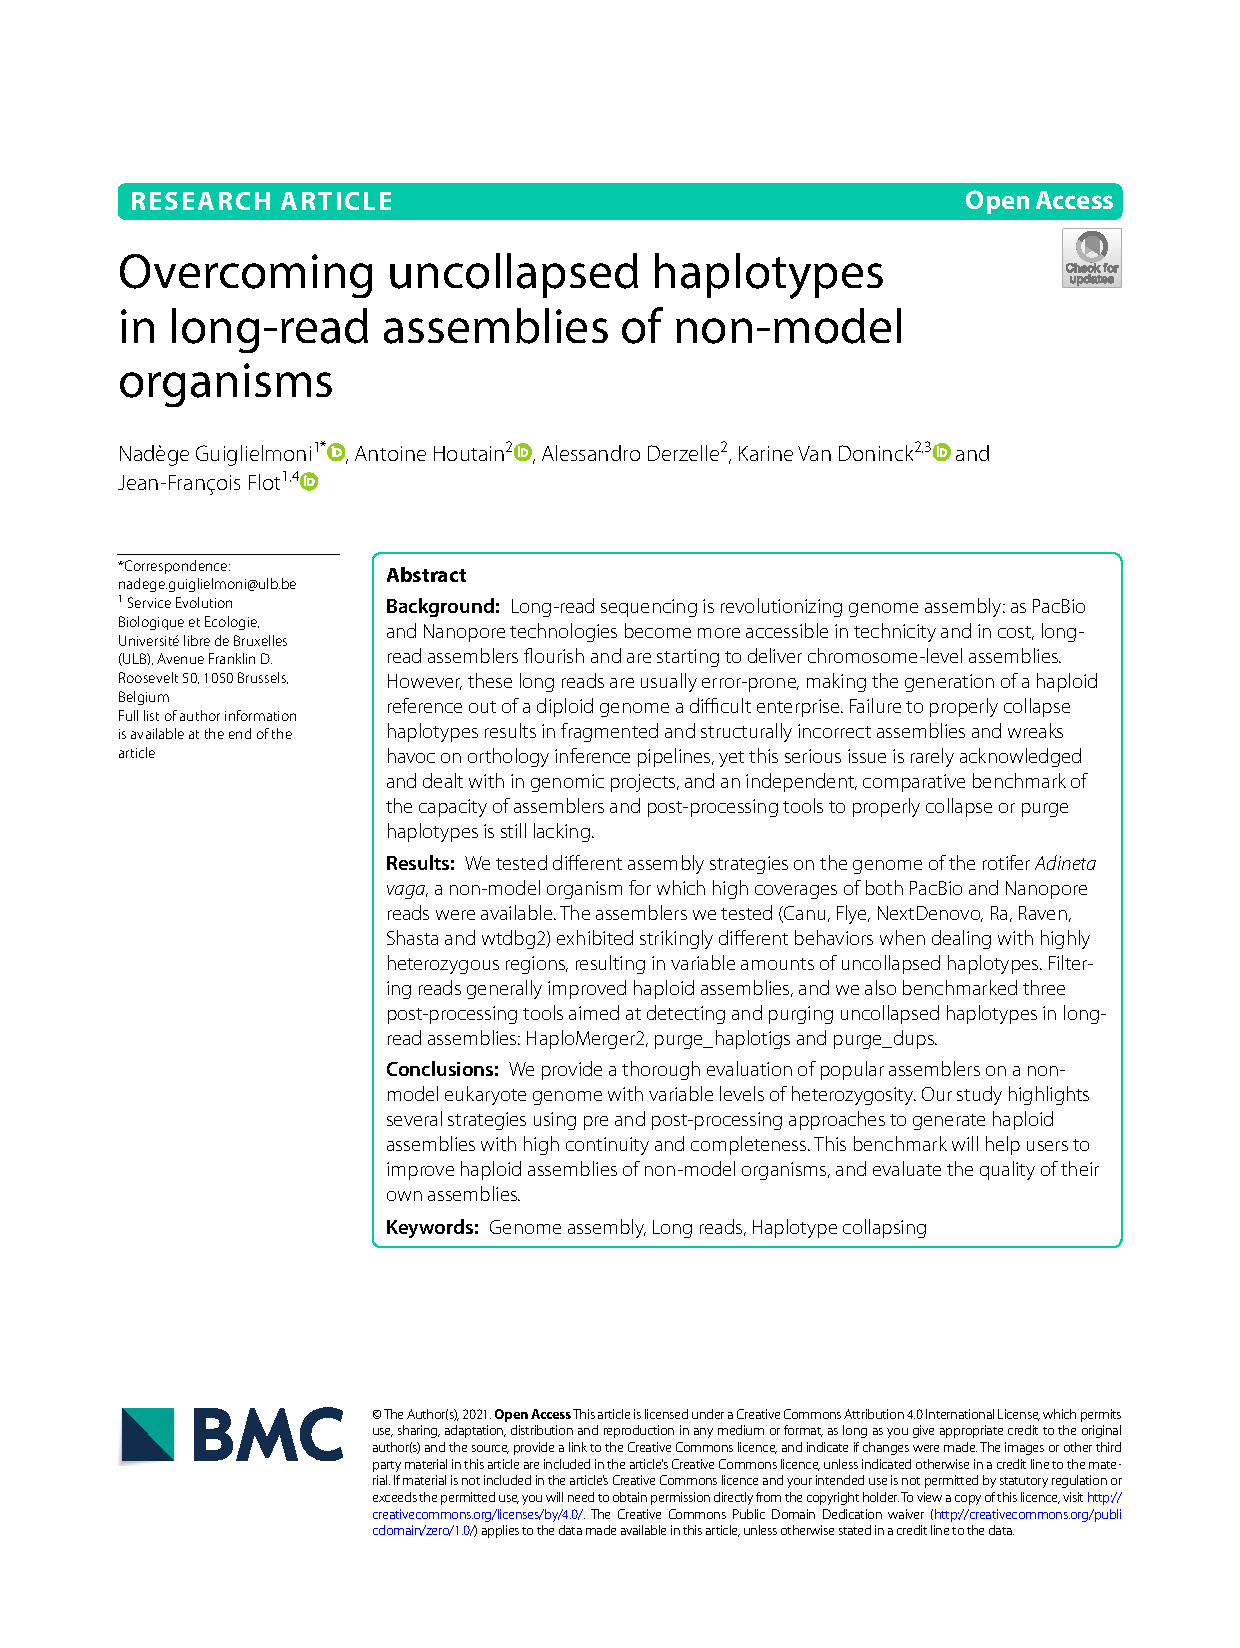
\includepdf[pages=-, pagecommand={}]{articles/benchmark.pdf}

\begin{suppsection}

\beginsupplement

\section*{Supplementary data}

   \begin{figure}[ht]
    \centering
     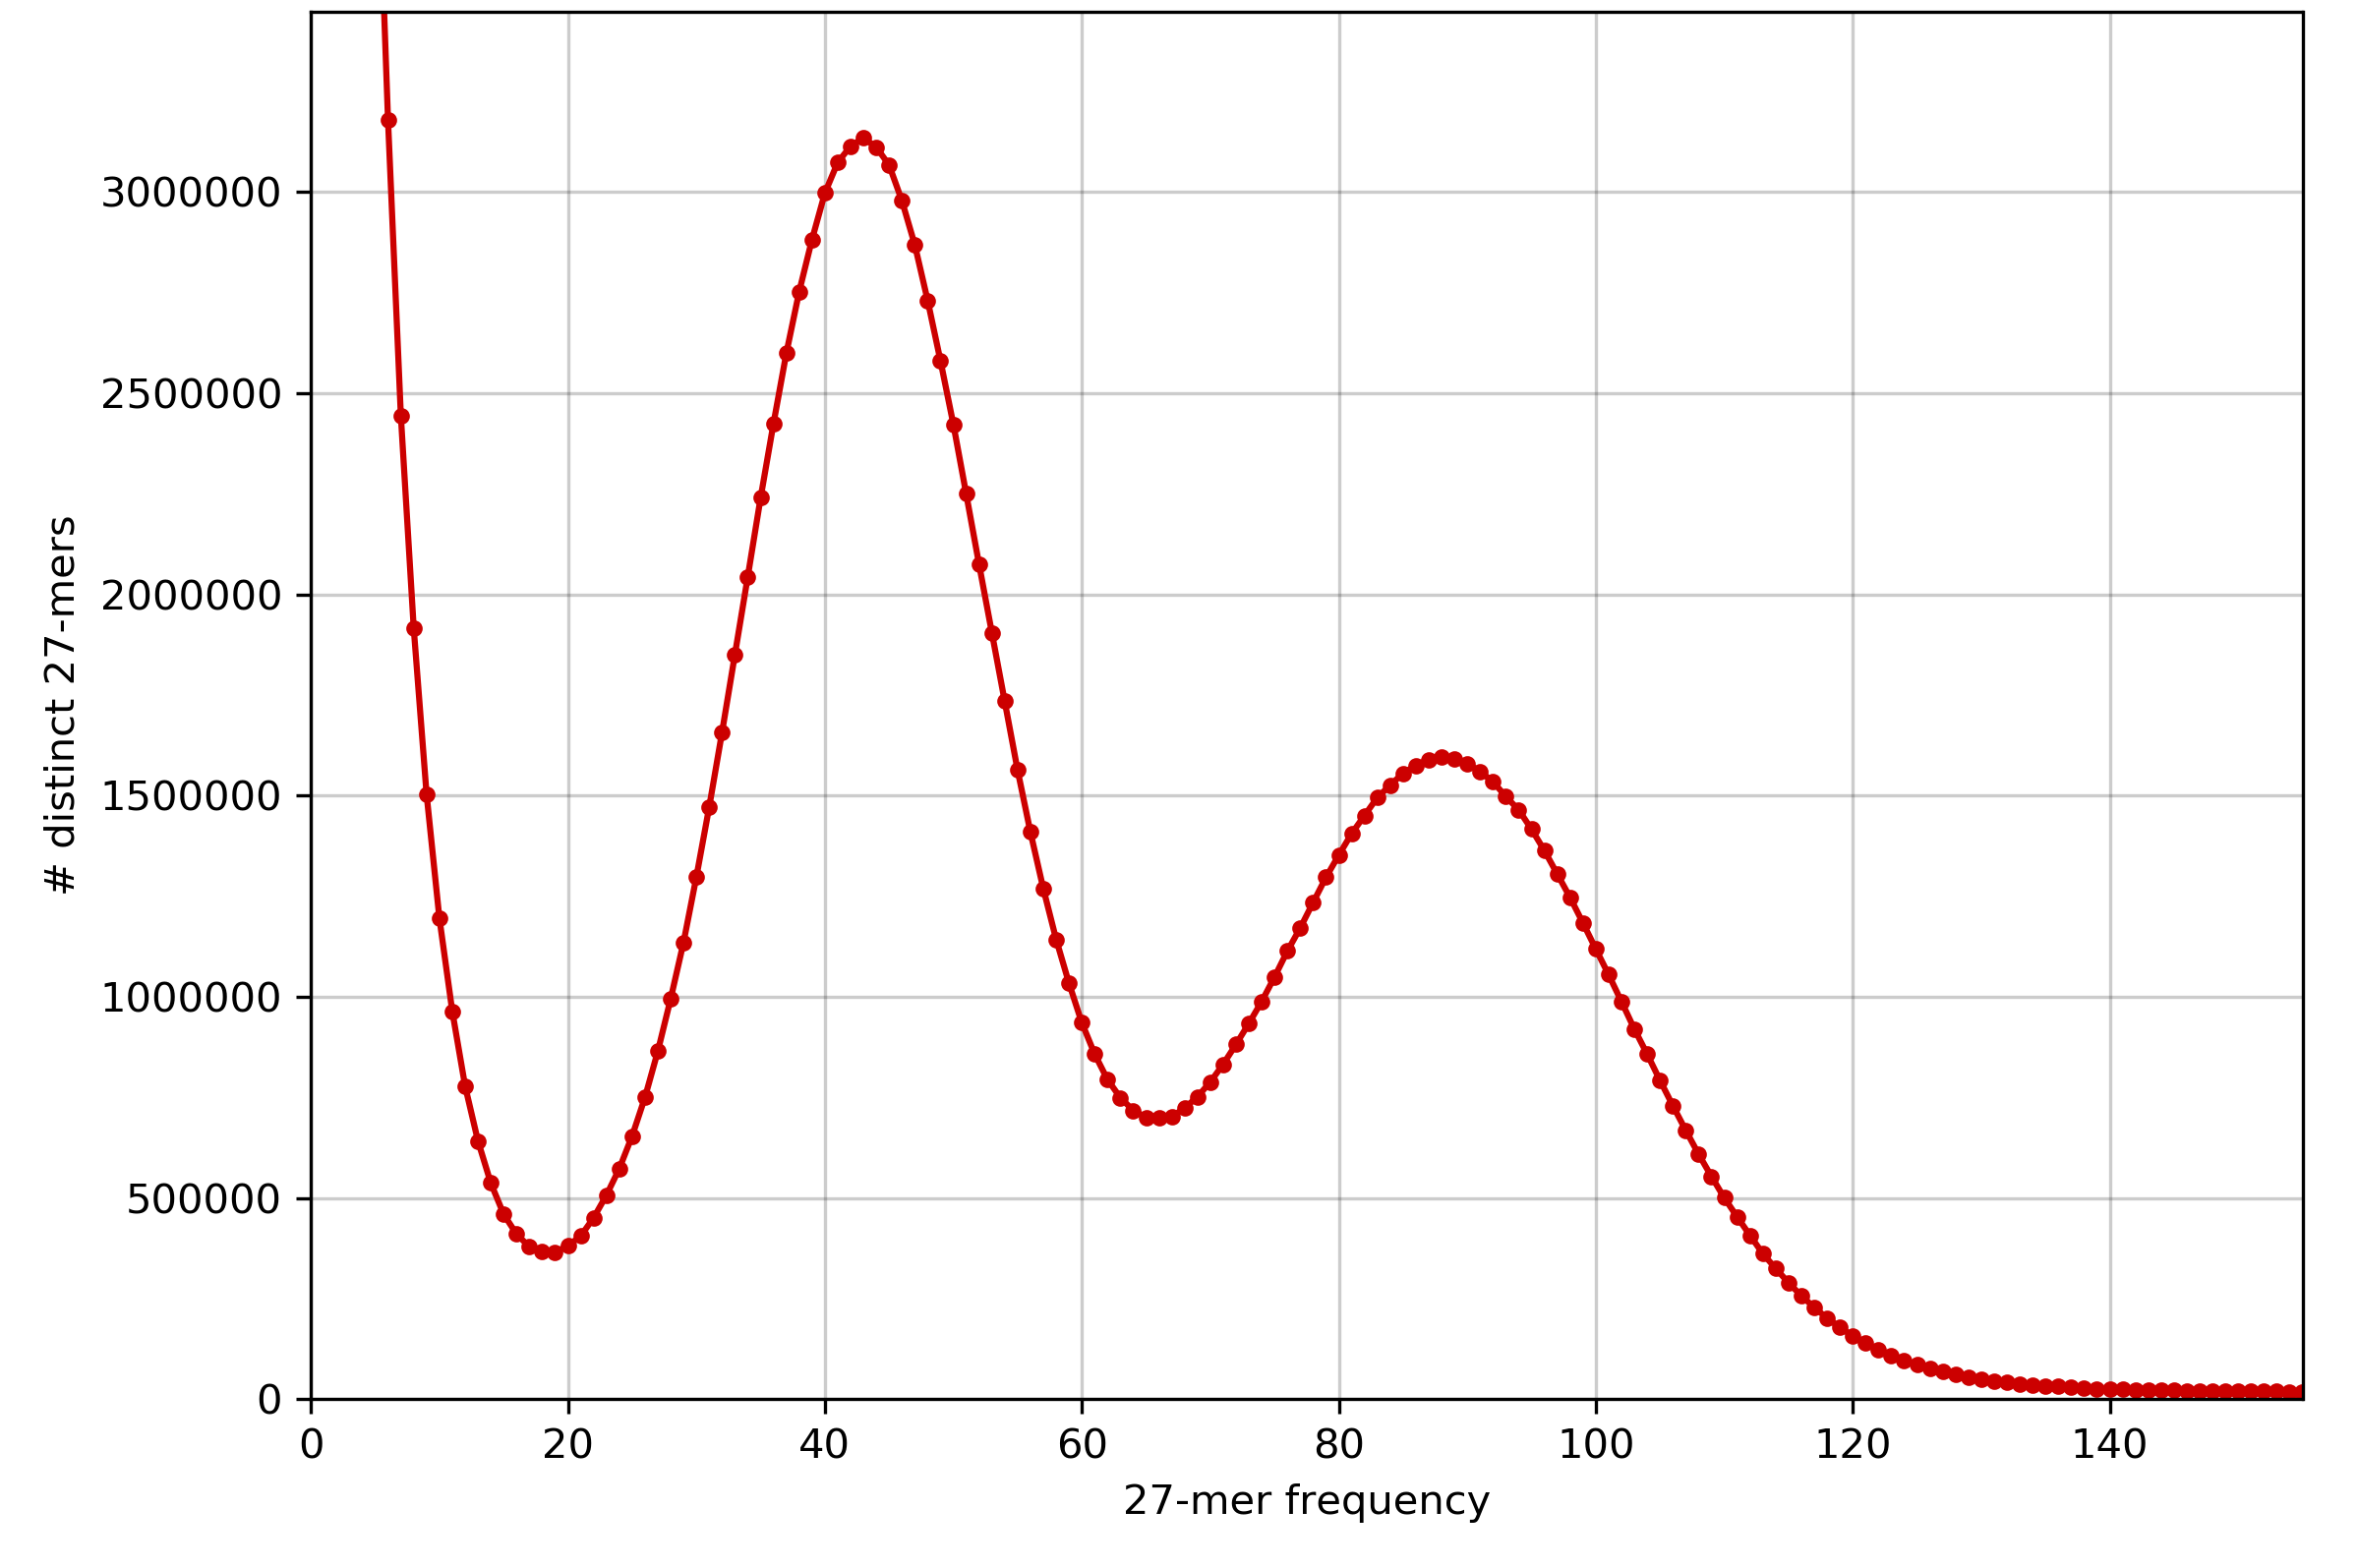
\includegraphics[width=13.5cm]{fig/benchmark/avaga_lab_kat.hist.png}
   \caption{\textit{k}-mer spectrum of \textit{Adineta vaga} using Illumina reads and KAT v2.4.2. The first peak corresponds to heterozygous \textit{k}-mers (around 45X) and the second peak corresponds to homozygous \textit{k}-mers.}
   \label{fig:kmer_spectrum}
 \end{figure}

   \begin{figure}[ht]
    \centering
     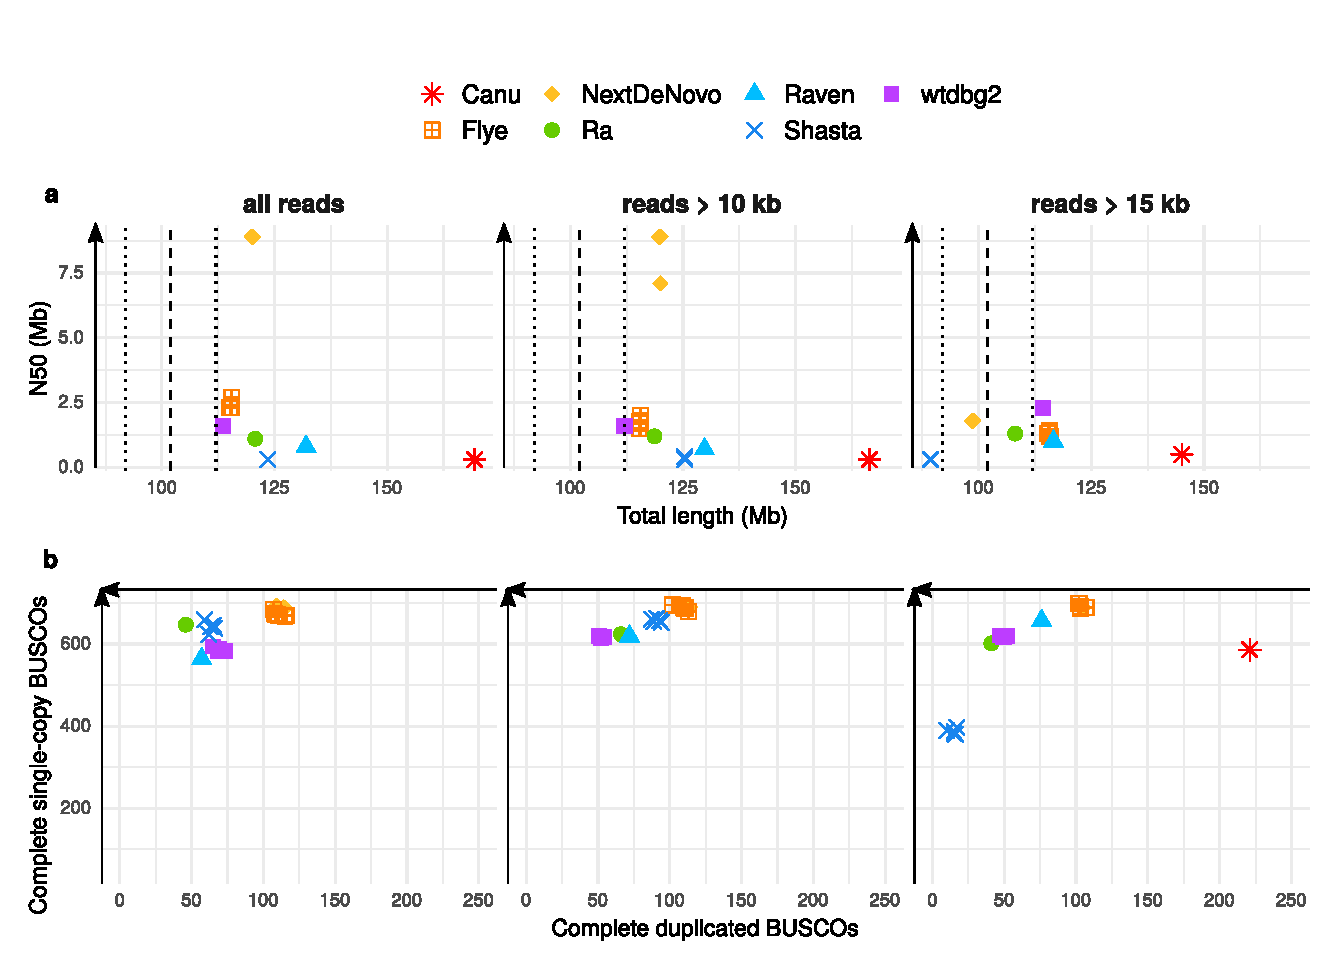
\includegraphics[width=13.5cm]{fig/benchmark/supp_pacbio_replicates.eps}
   \caption{Statistics of PacBio assemblies obtained from the full PacBio dataset or with a read-filtering step prior to assembly based on read length exclusively, using different thresholds: 10 kb, 15 kb. All assemblies were run five times to assess the reproducibility of the output produced by each assembler. a) N50 plotted against total assembly length. The dashed line indicates the expected genome size, with a +/- 10 Mb margin delimited by the dotted lines. b) Number of complete single-copy BUSCOs plotted against number of complete duplicated BUSCOs, from a total of 954 orthologs.}
   \label{fig:pacbio_replicates}
 \end{figure}
 
    \begin{figure}[ht]
    \centering
     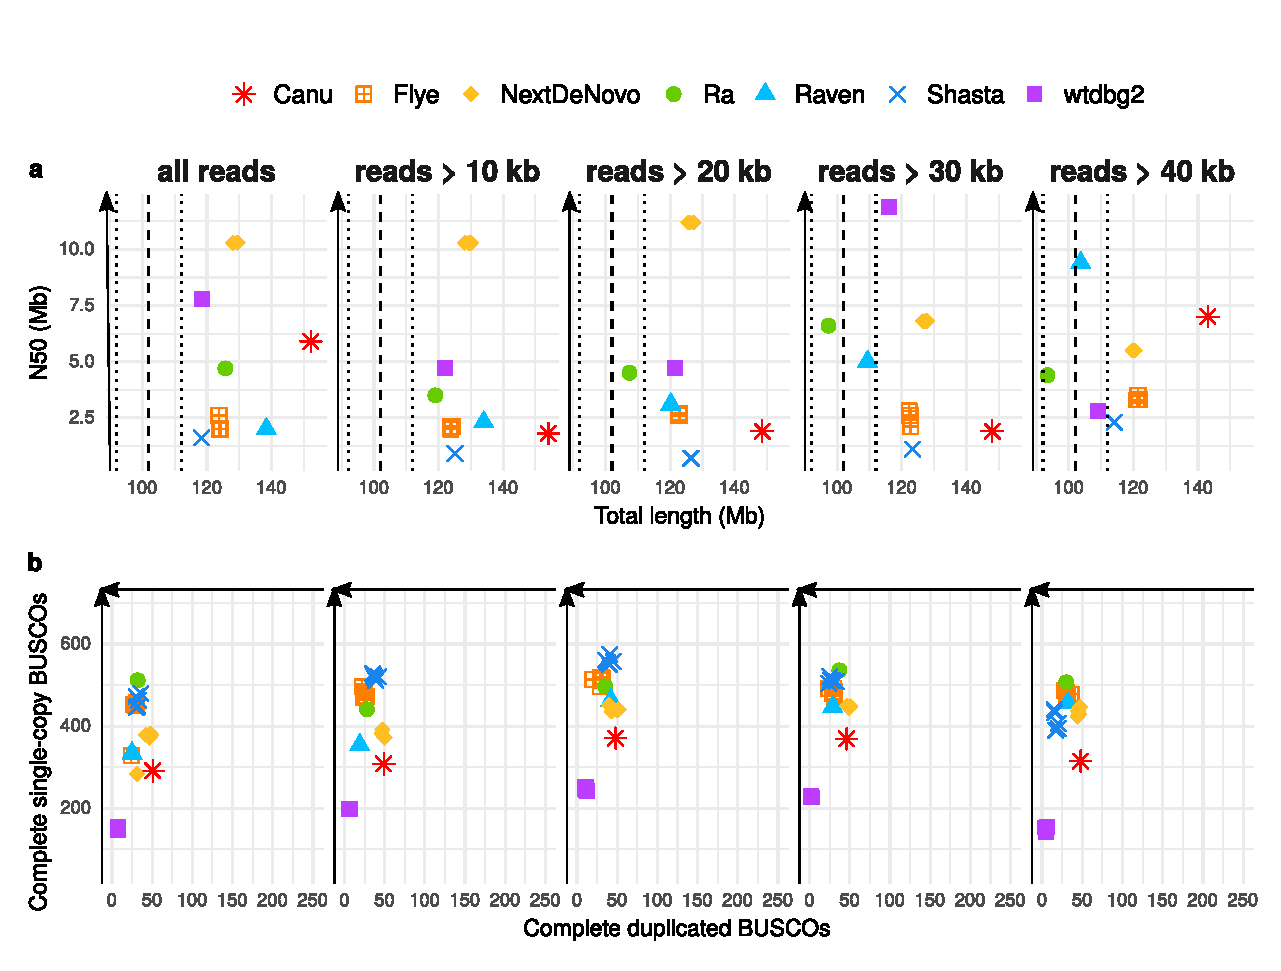
\includegraphics[width=13.5cm]{fig/benchmark/supp_nanopore_replicates.eps}
   \caption{Statistics of Nanopore assemblies obtained from the full Nanopore dataset or with a read-filtering step prior to assembly based on read length exclusively, using different thresholds: 10 kb, 20 kb, 30 kb, 40 kb. All assemblies were run five times to assess the reproducibility of the output produced by each assembler. a) N50 plotted against total assembly length. The dashed line indicates the expected genome size, with +/- 10 Mb margin delimited by the dotted lines. b) Number of complete single-copy BUSCOs plotted against number of complete duplicated BUSCOs, from a total of 954 orthologs.}
   \label{fig:nanopore_replicates}
 \end{figure}

   \begin{figure}[ht]
    \centering
     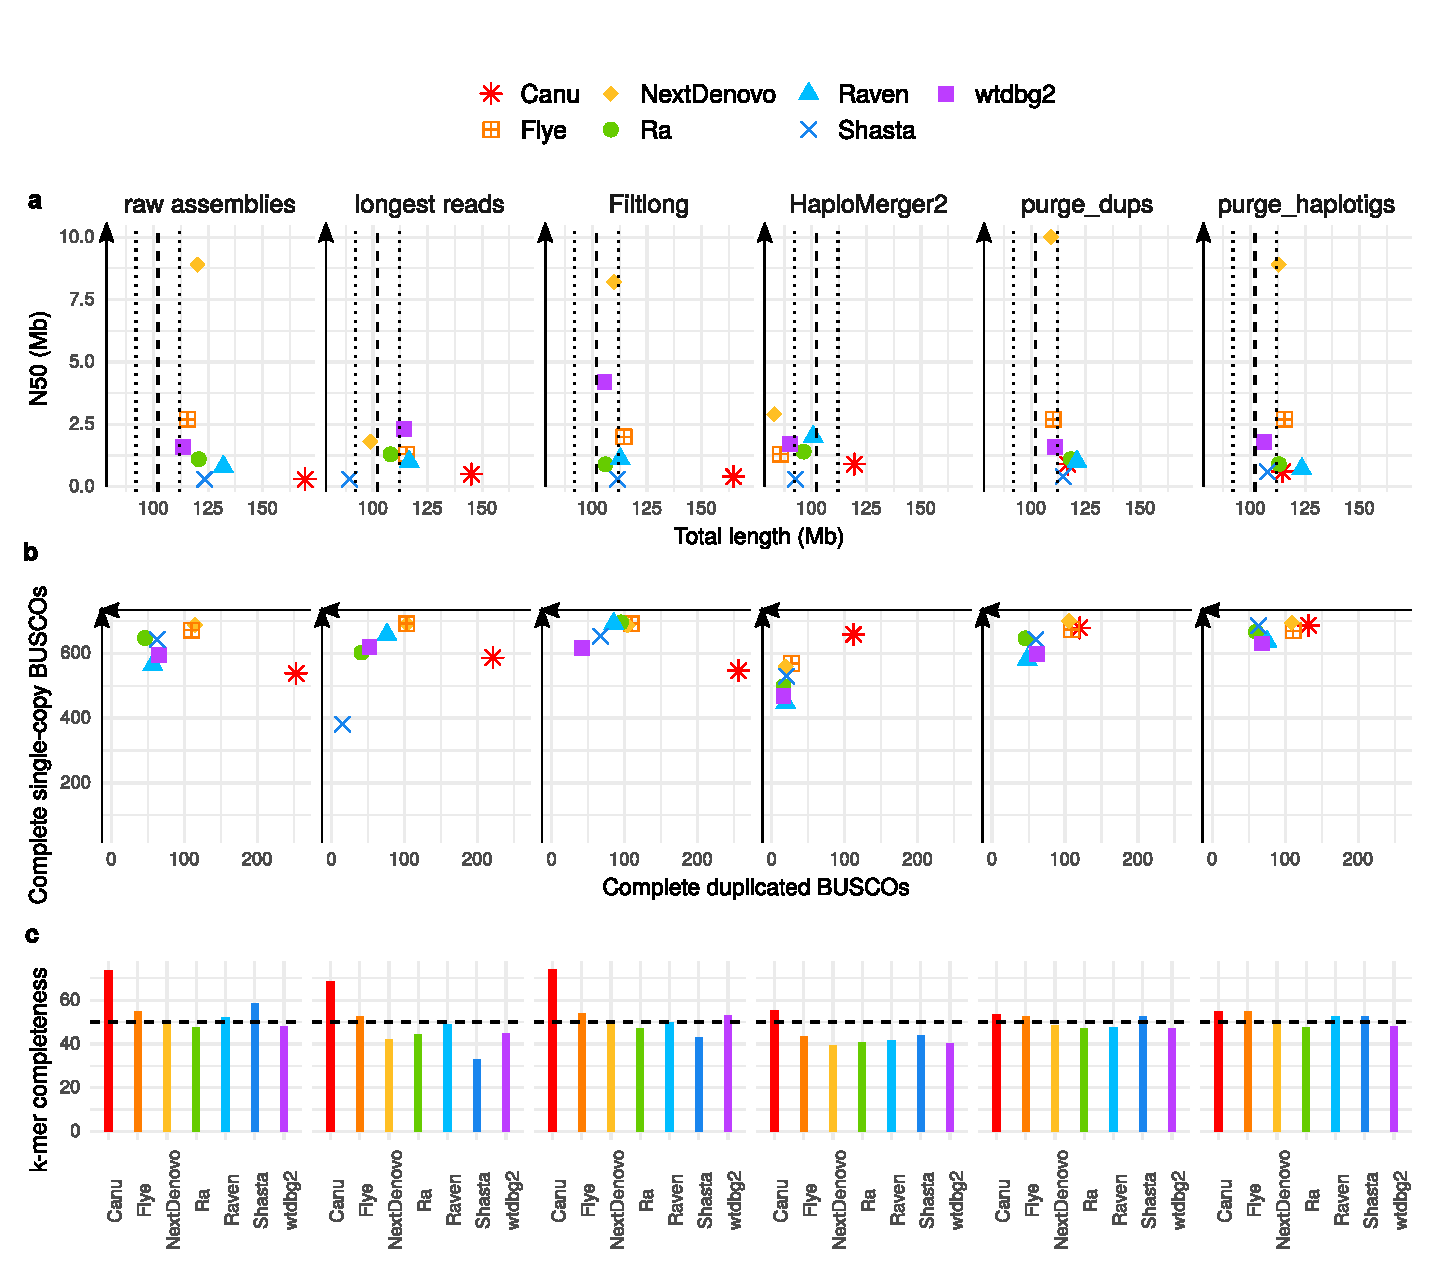
\includegraphics[width=13.5cm]{fig/benchmark/pacbio_all_v20210317.eps}
   \caption{Statistics of raw assemblies obtained from the full PacBio dataset (raw assemblies), with a preliminary read filtering step (keeping only reads larger than 15 kb, or those selected by Filtlong based on quality and length) or a subsequent removal of uncollapsed haplotypes with HaploMerger2, purge\_dups, or purge\_haplotigs. a) N50 plotted against total assembly length. The dashed line indicates the expected genome size, with +/- 10 Mb margin delimited by the dotted lines. b) Number of complete single-copy BUSCOs plotted against number of complete duplicated BUSCOs, from a total of 954 orthologs. c) \textit{k}-mer completeness. The dashed line indicates the expected 50\% completeness.}
   \label{fig:pacbio_full_stats}
 \end{figure}
 
  \begin{figure}[ht]
    \centering
     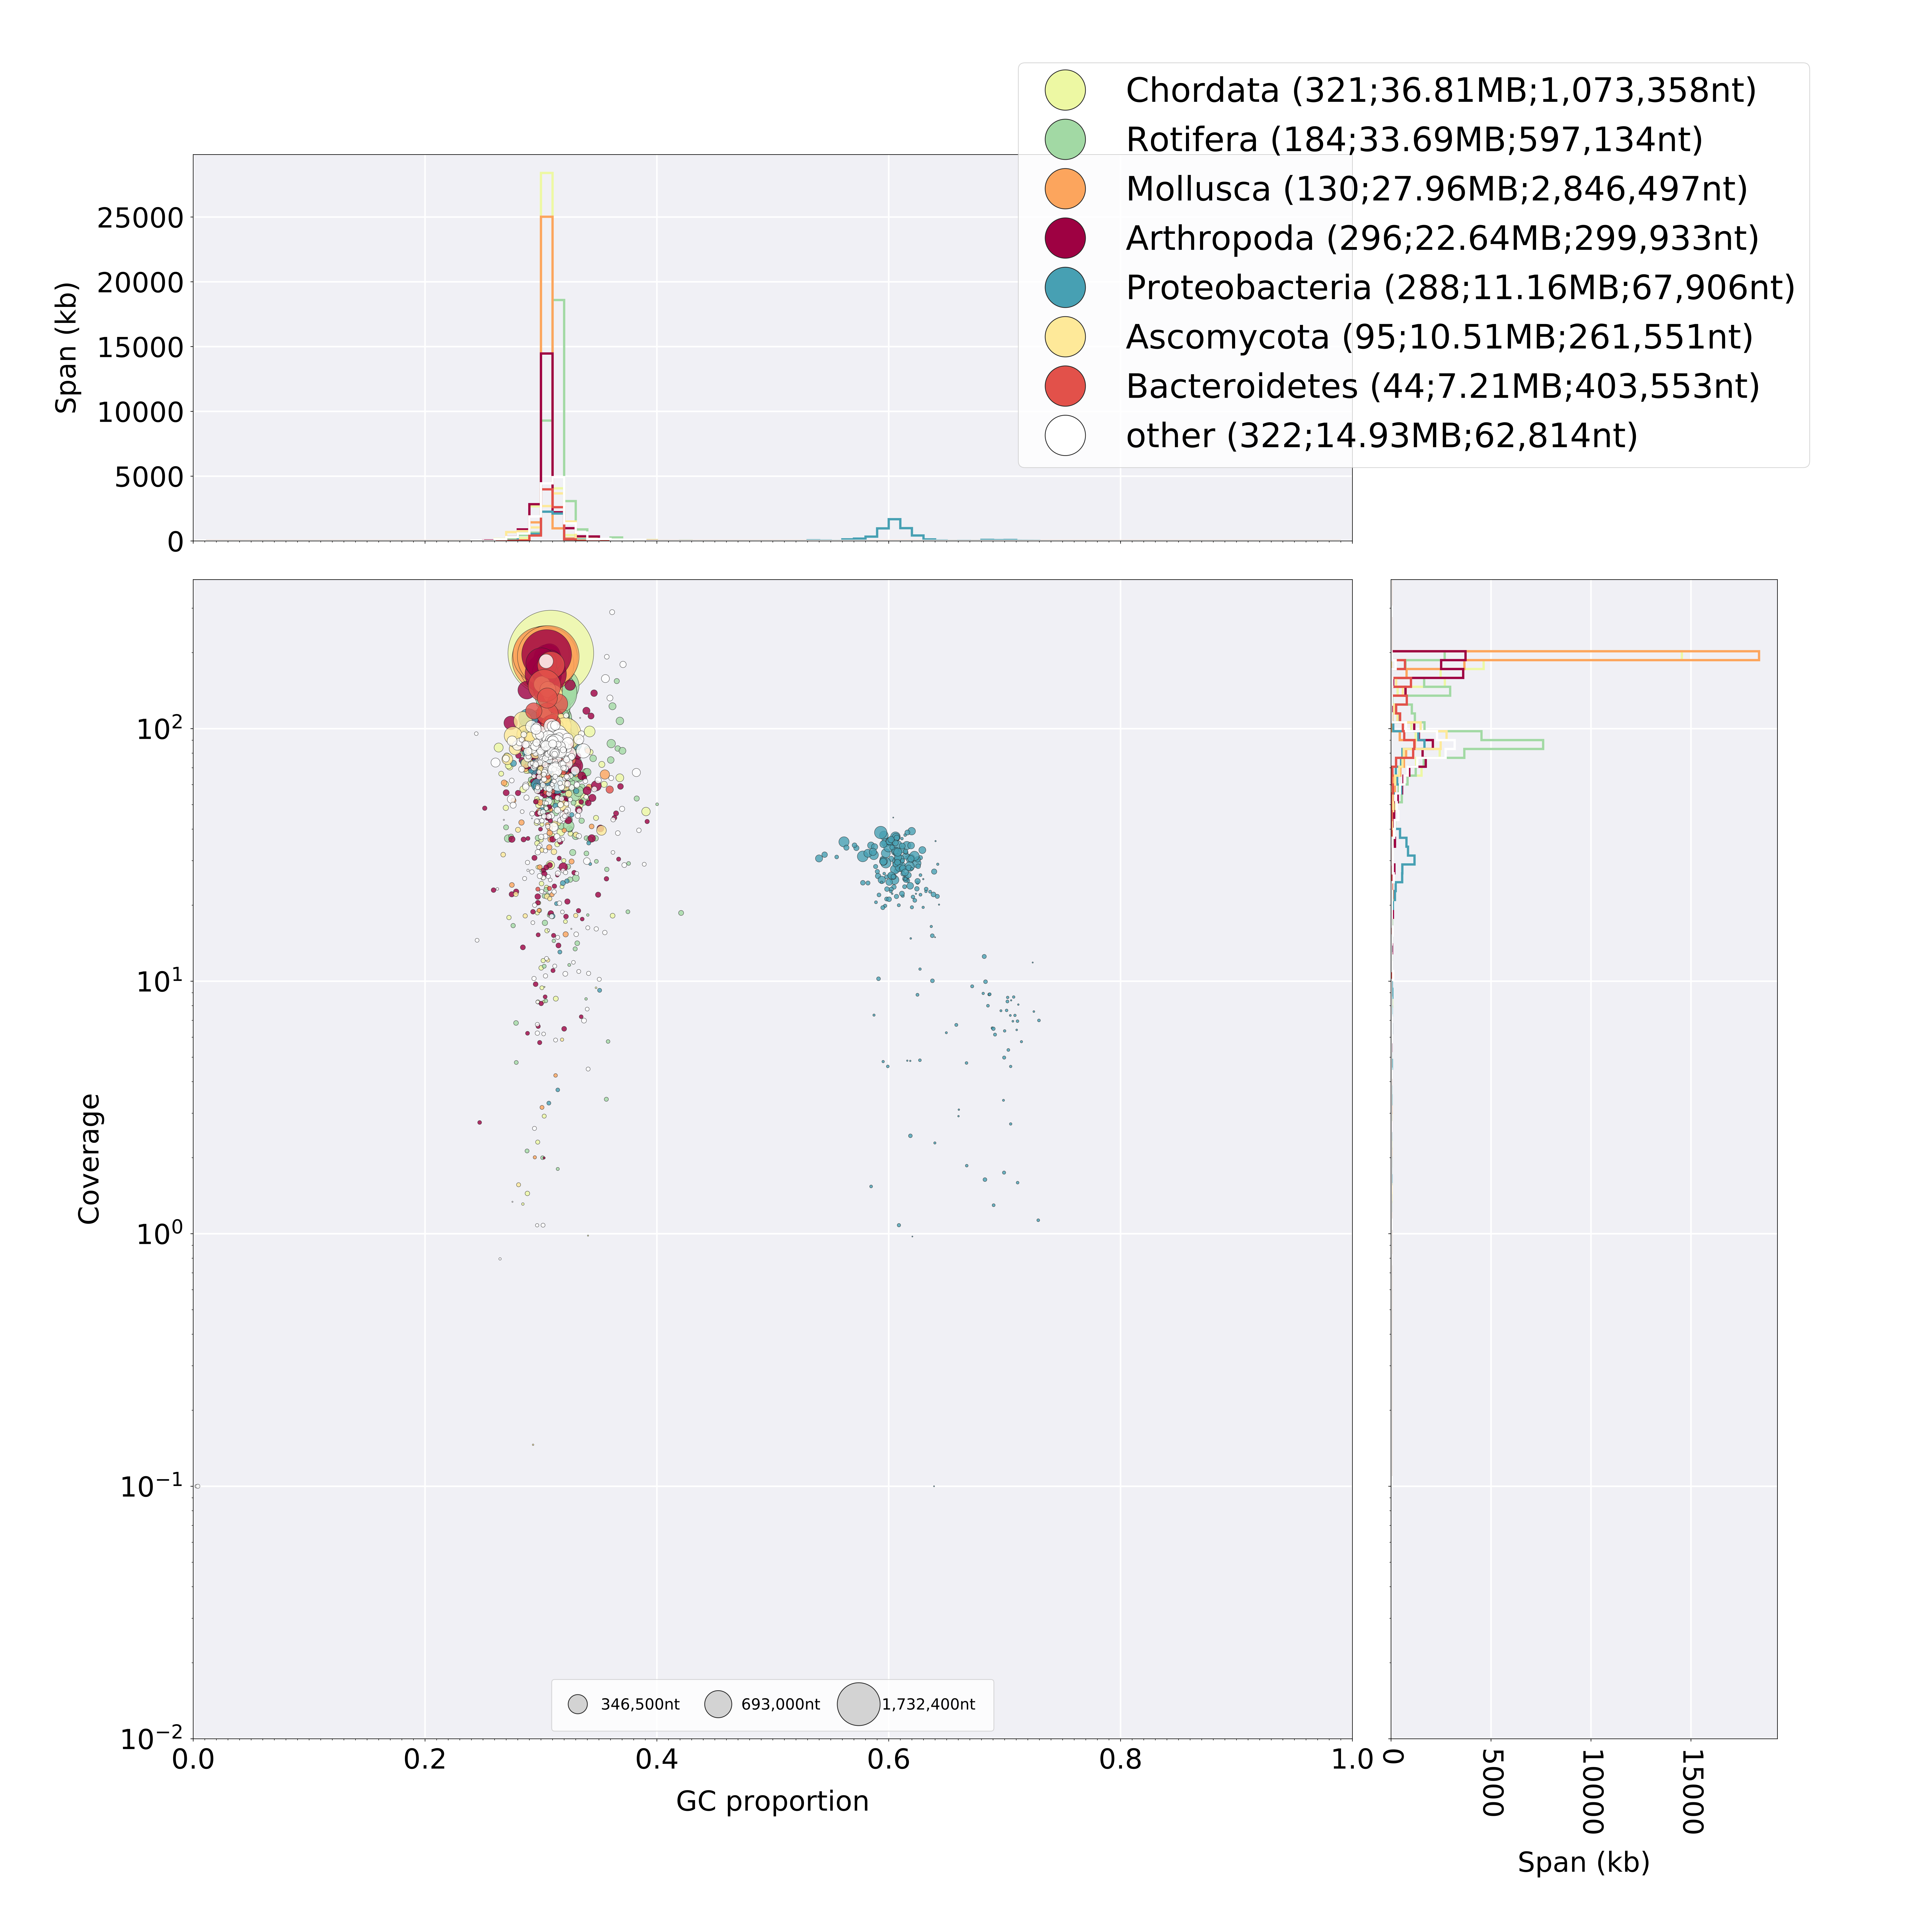
\includegraphics[width=15cm]{fig/benchmark/PB_CANU.png}
   \caption{Blobtools v1.0 analysis of a Canu assembly of the full PacBio dataset.}
   \label{fig:blobtools_canu_pb}
 \end{figure}
 
 \begin{figure}[ht]
    \centering
     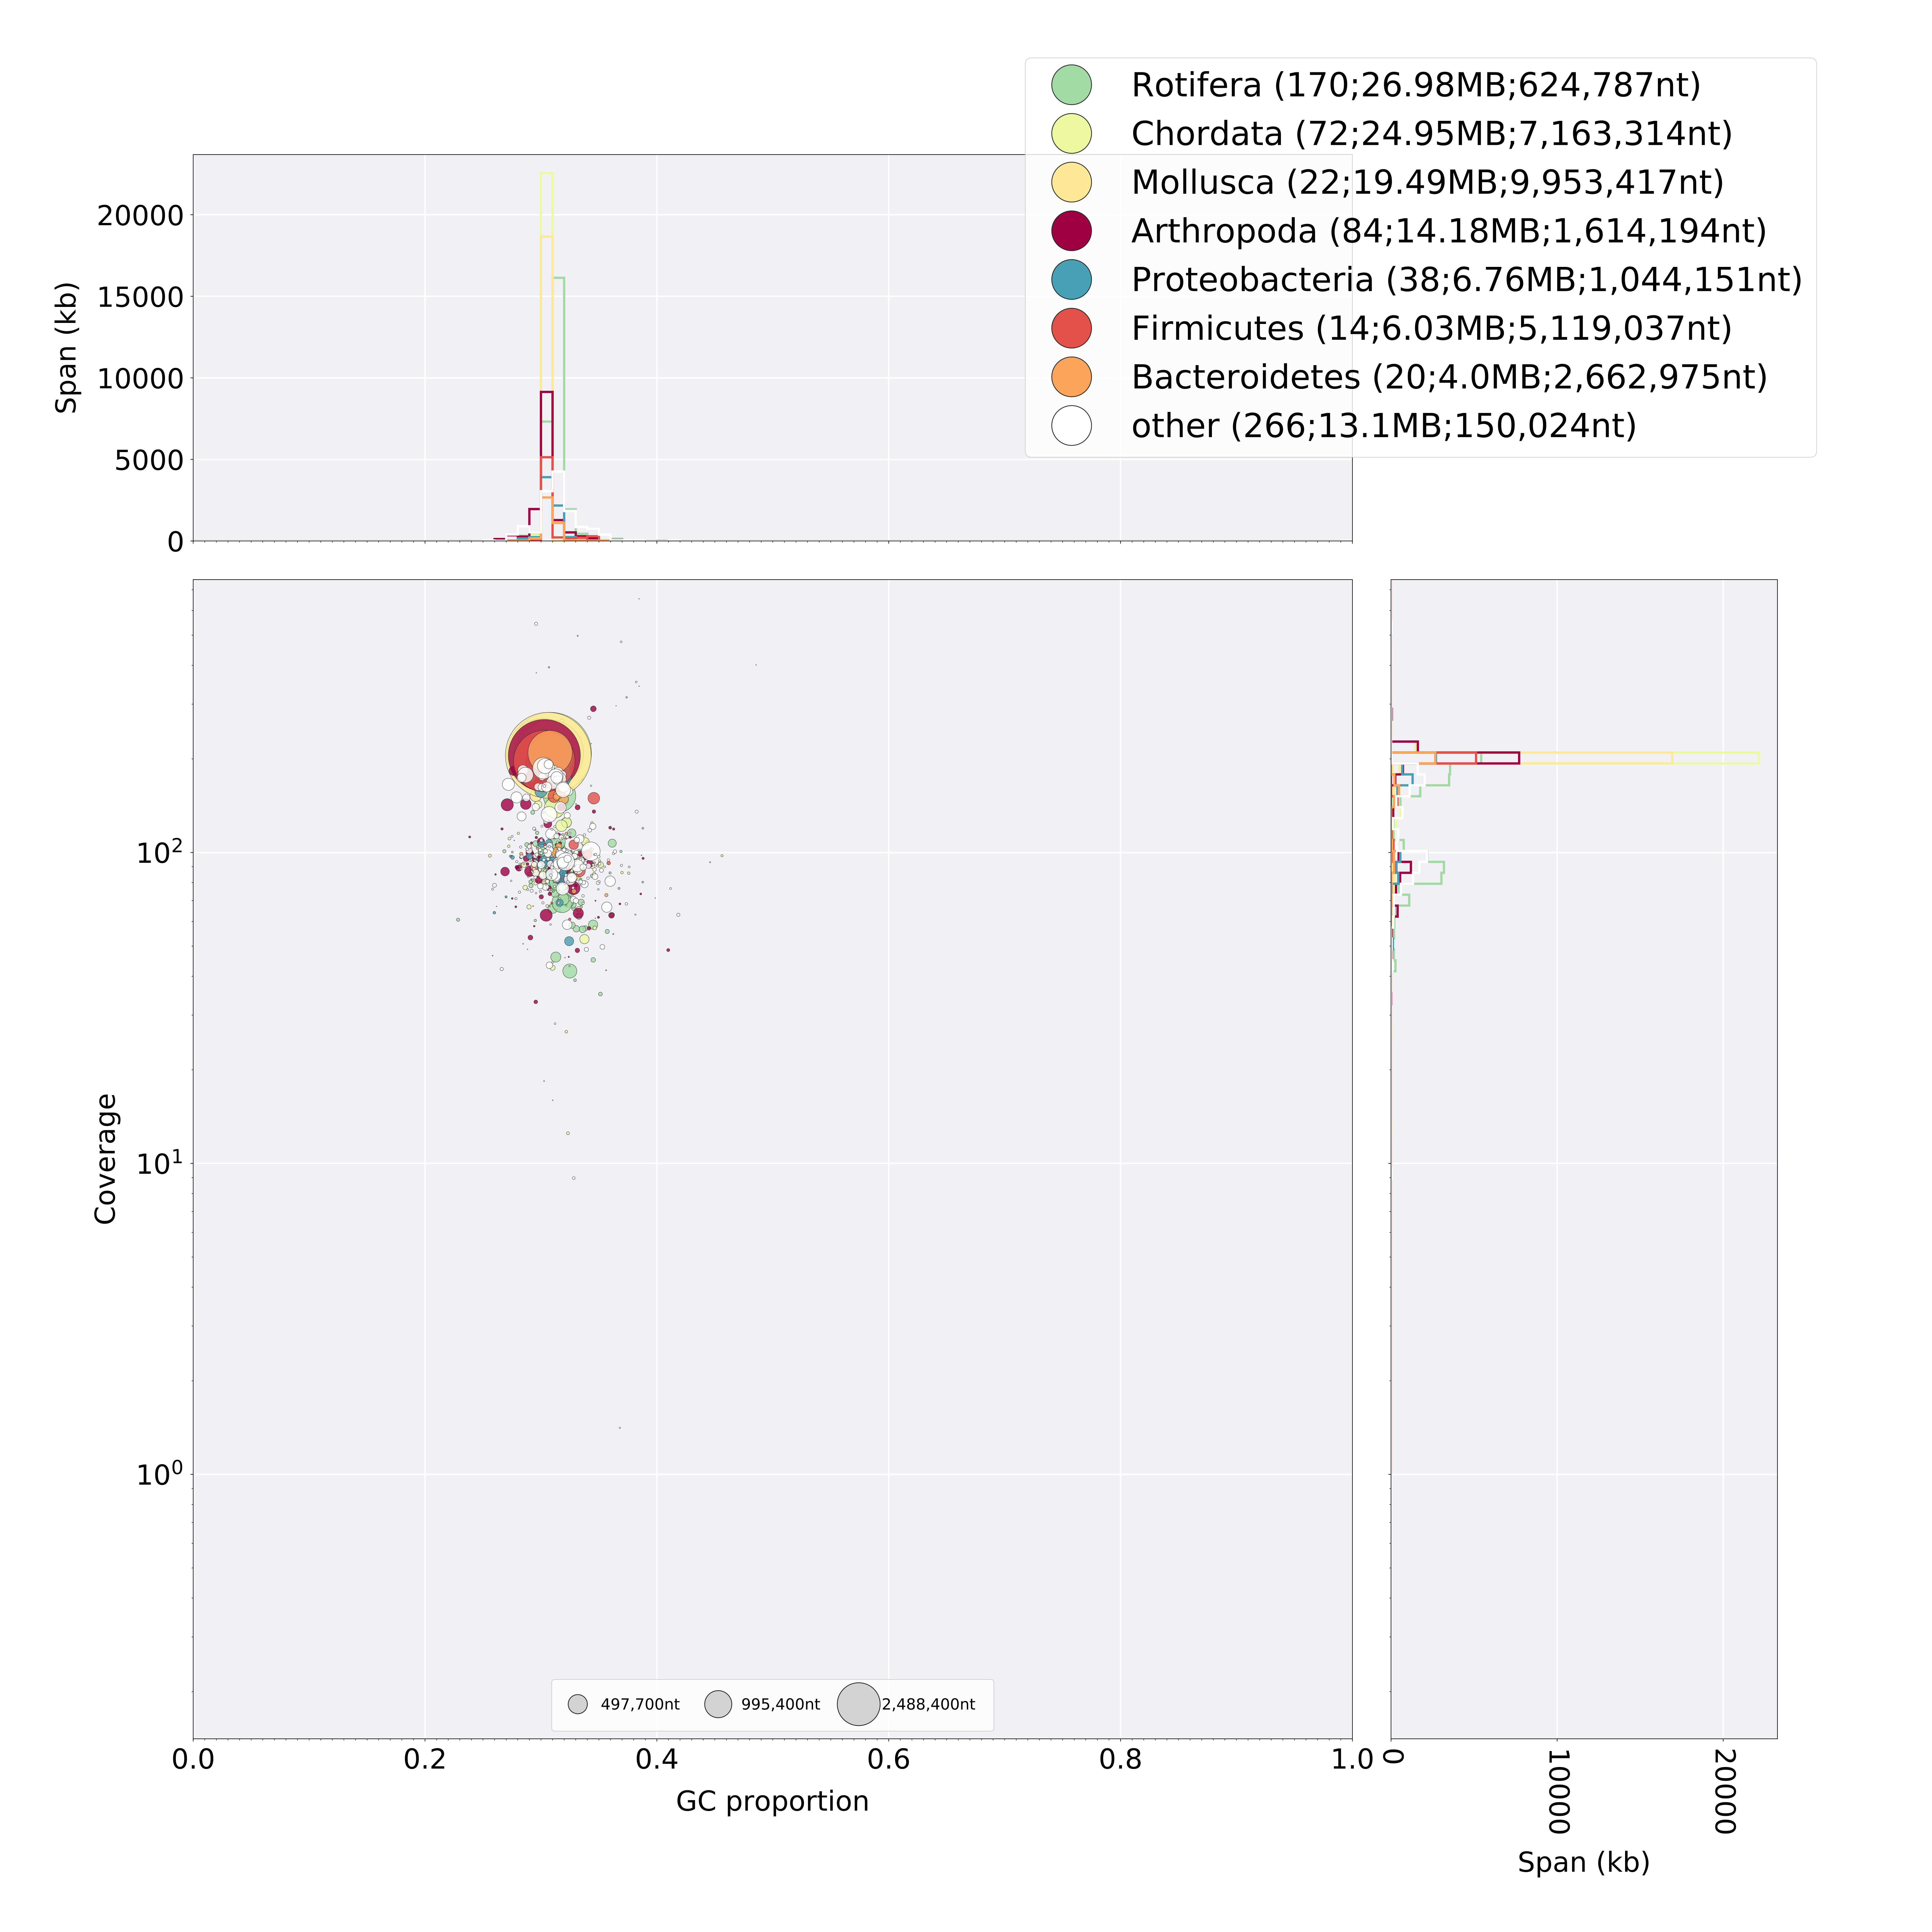
\includegraphics[width=15cm]{fig/benchmark/PB_FLYE.png}
   \caption{Blobtools v1.0 analysis of a Flye assembly of the full PacBio dataset.}
   \label{fig:blobtools_flye_pb}
 \end{figure}
 
  \begin{figure}[ht]
    \centering
     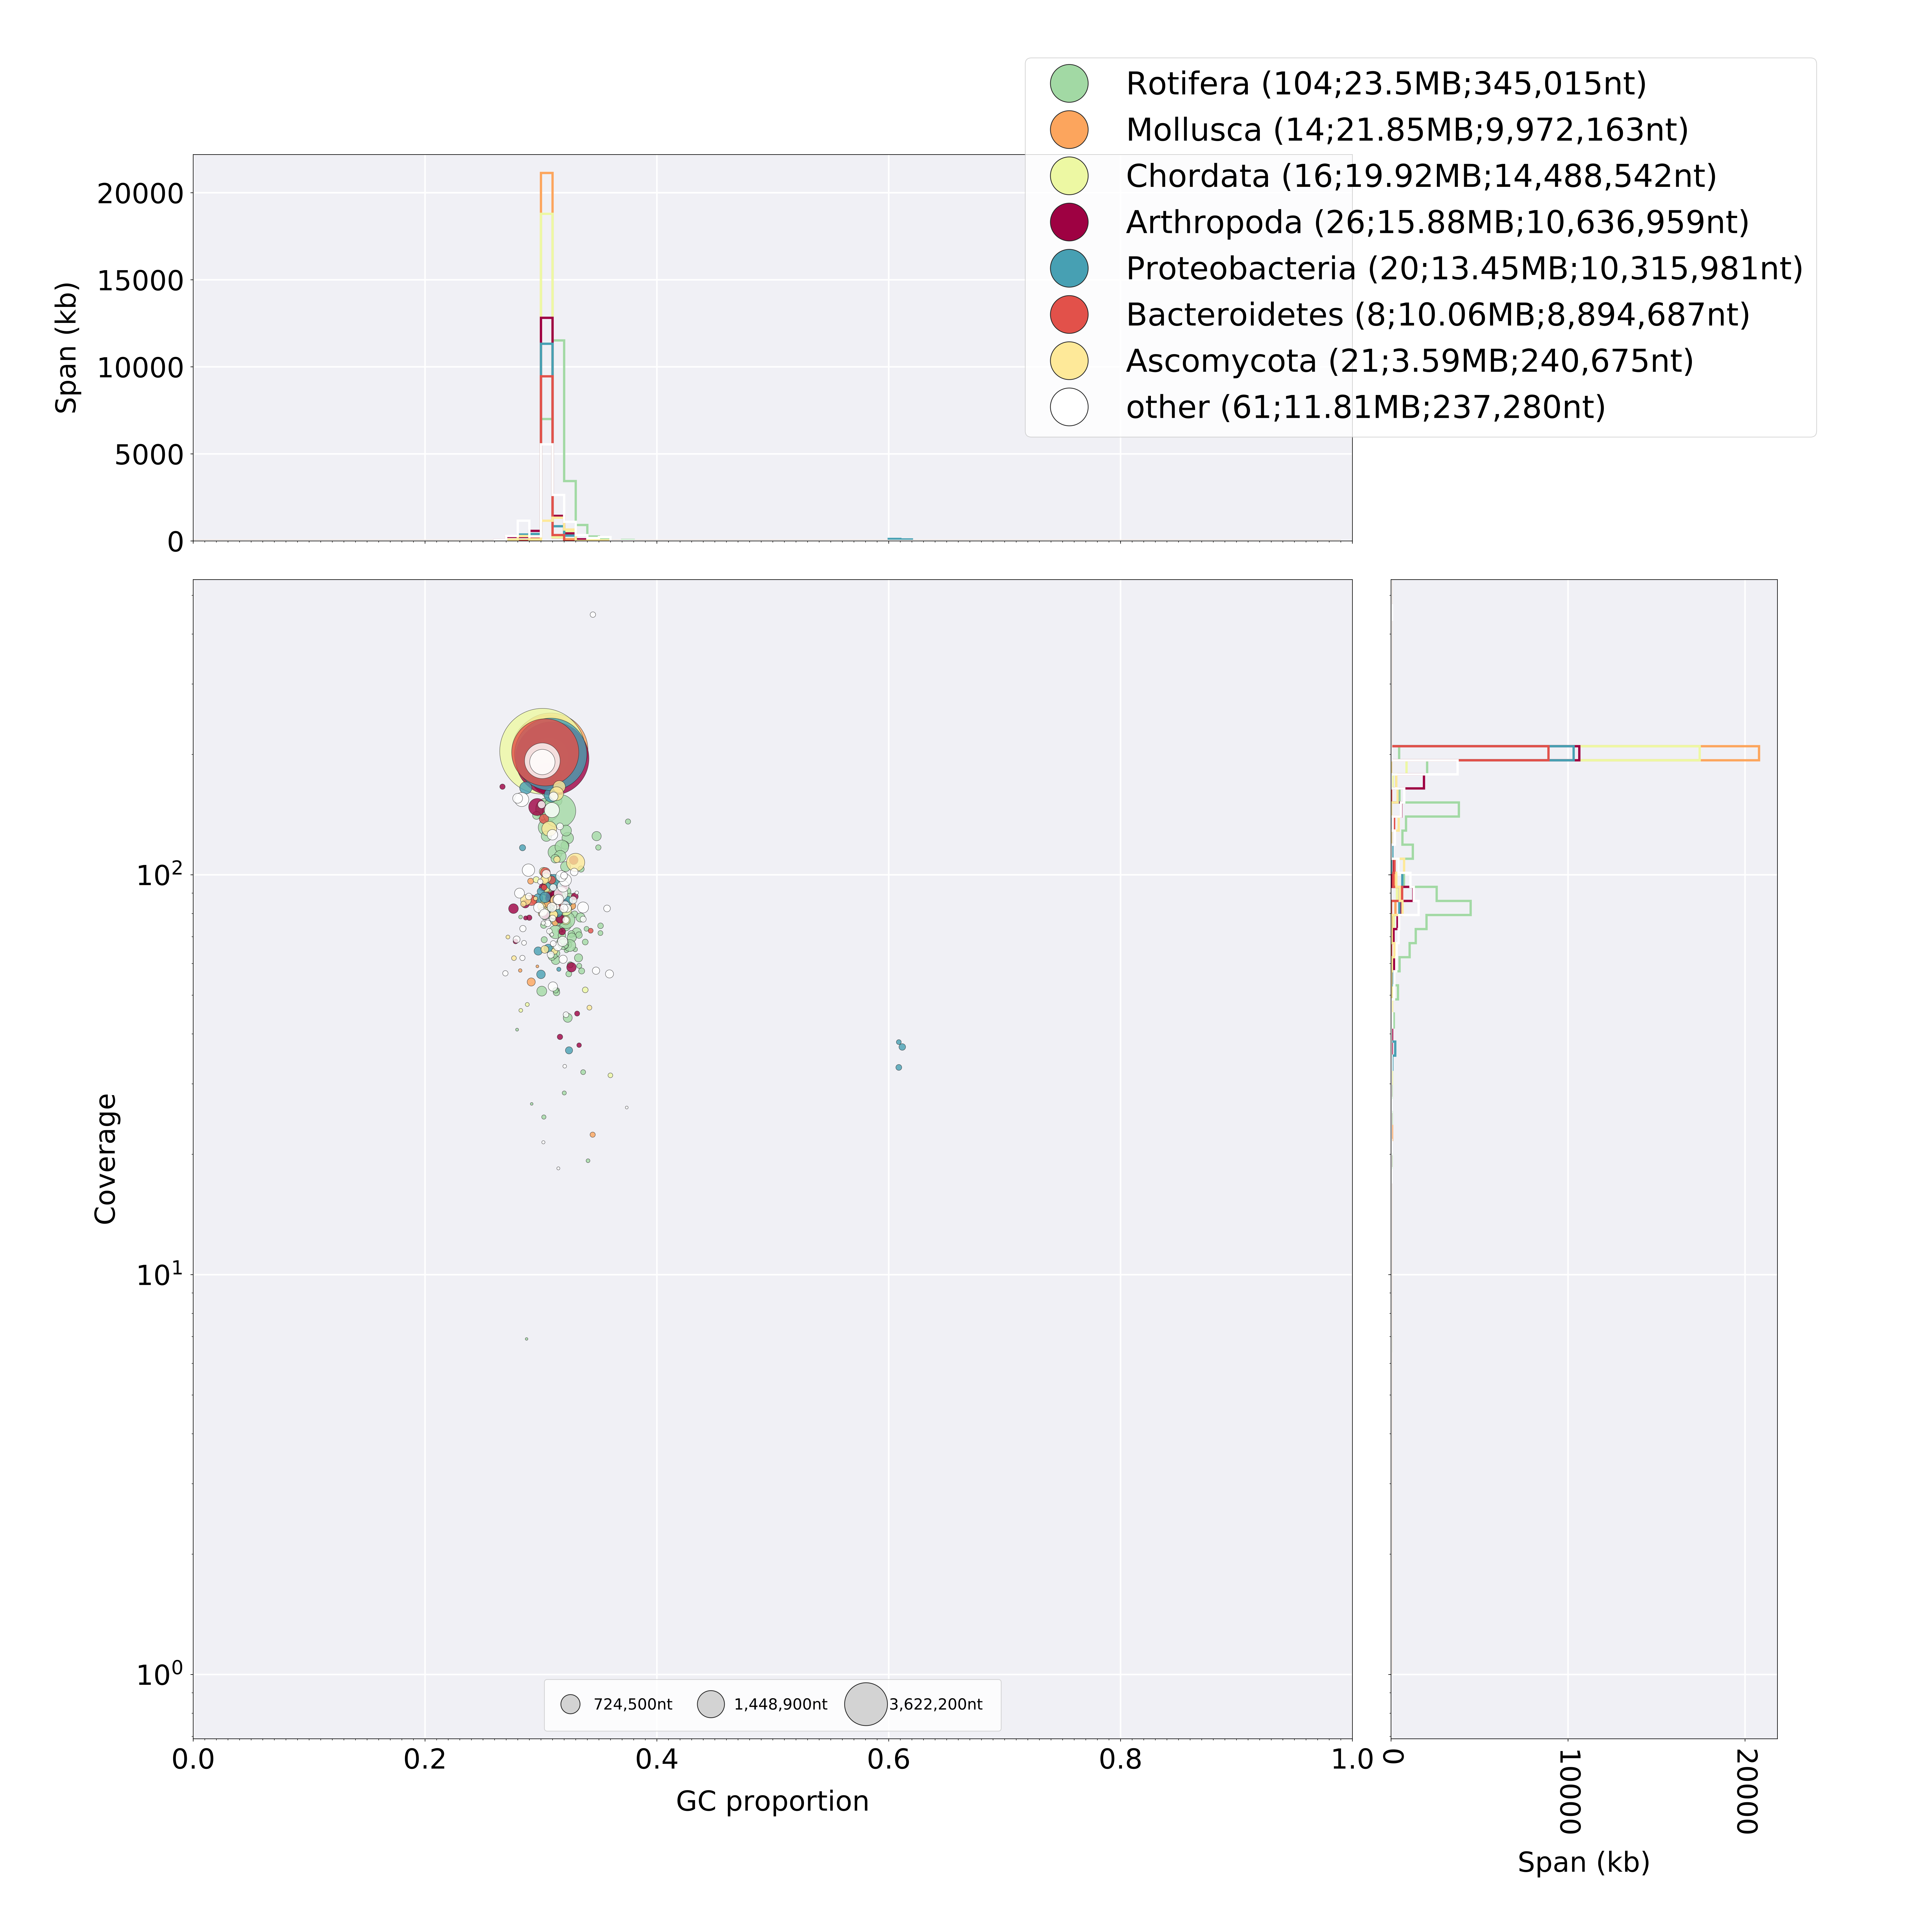
\includegraphics[width=15cm]{fig/benchmark/PB_ND.png}
   \caption{Blobtools v1.0 analysis of a NextDenovo assembly of the full PacBio dataset.}
   \label{fig:blobtools_NextDenovo_pb}
 \end{figure}

 \begin{figure}[ht]
    \centering
     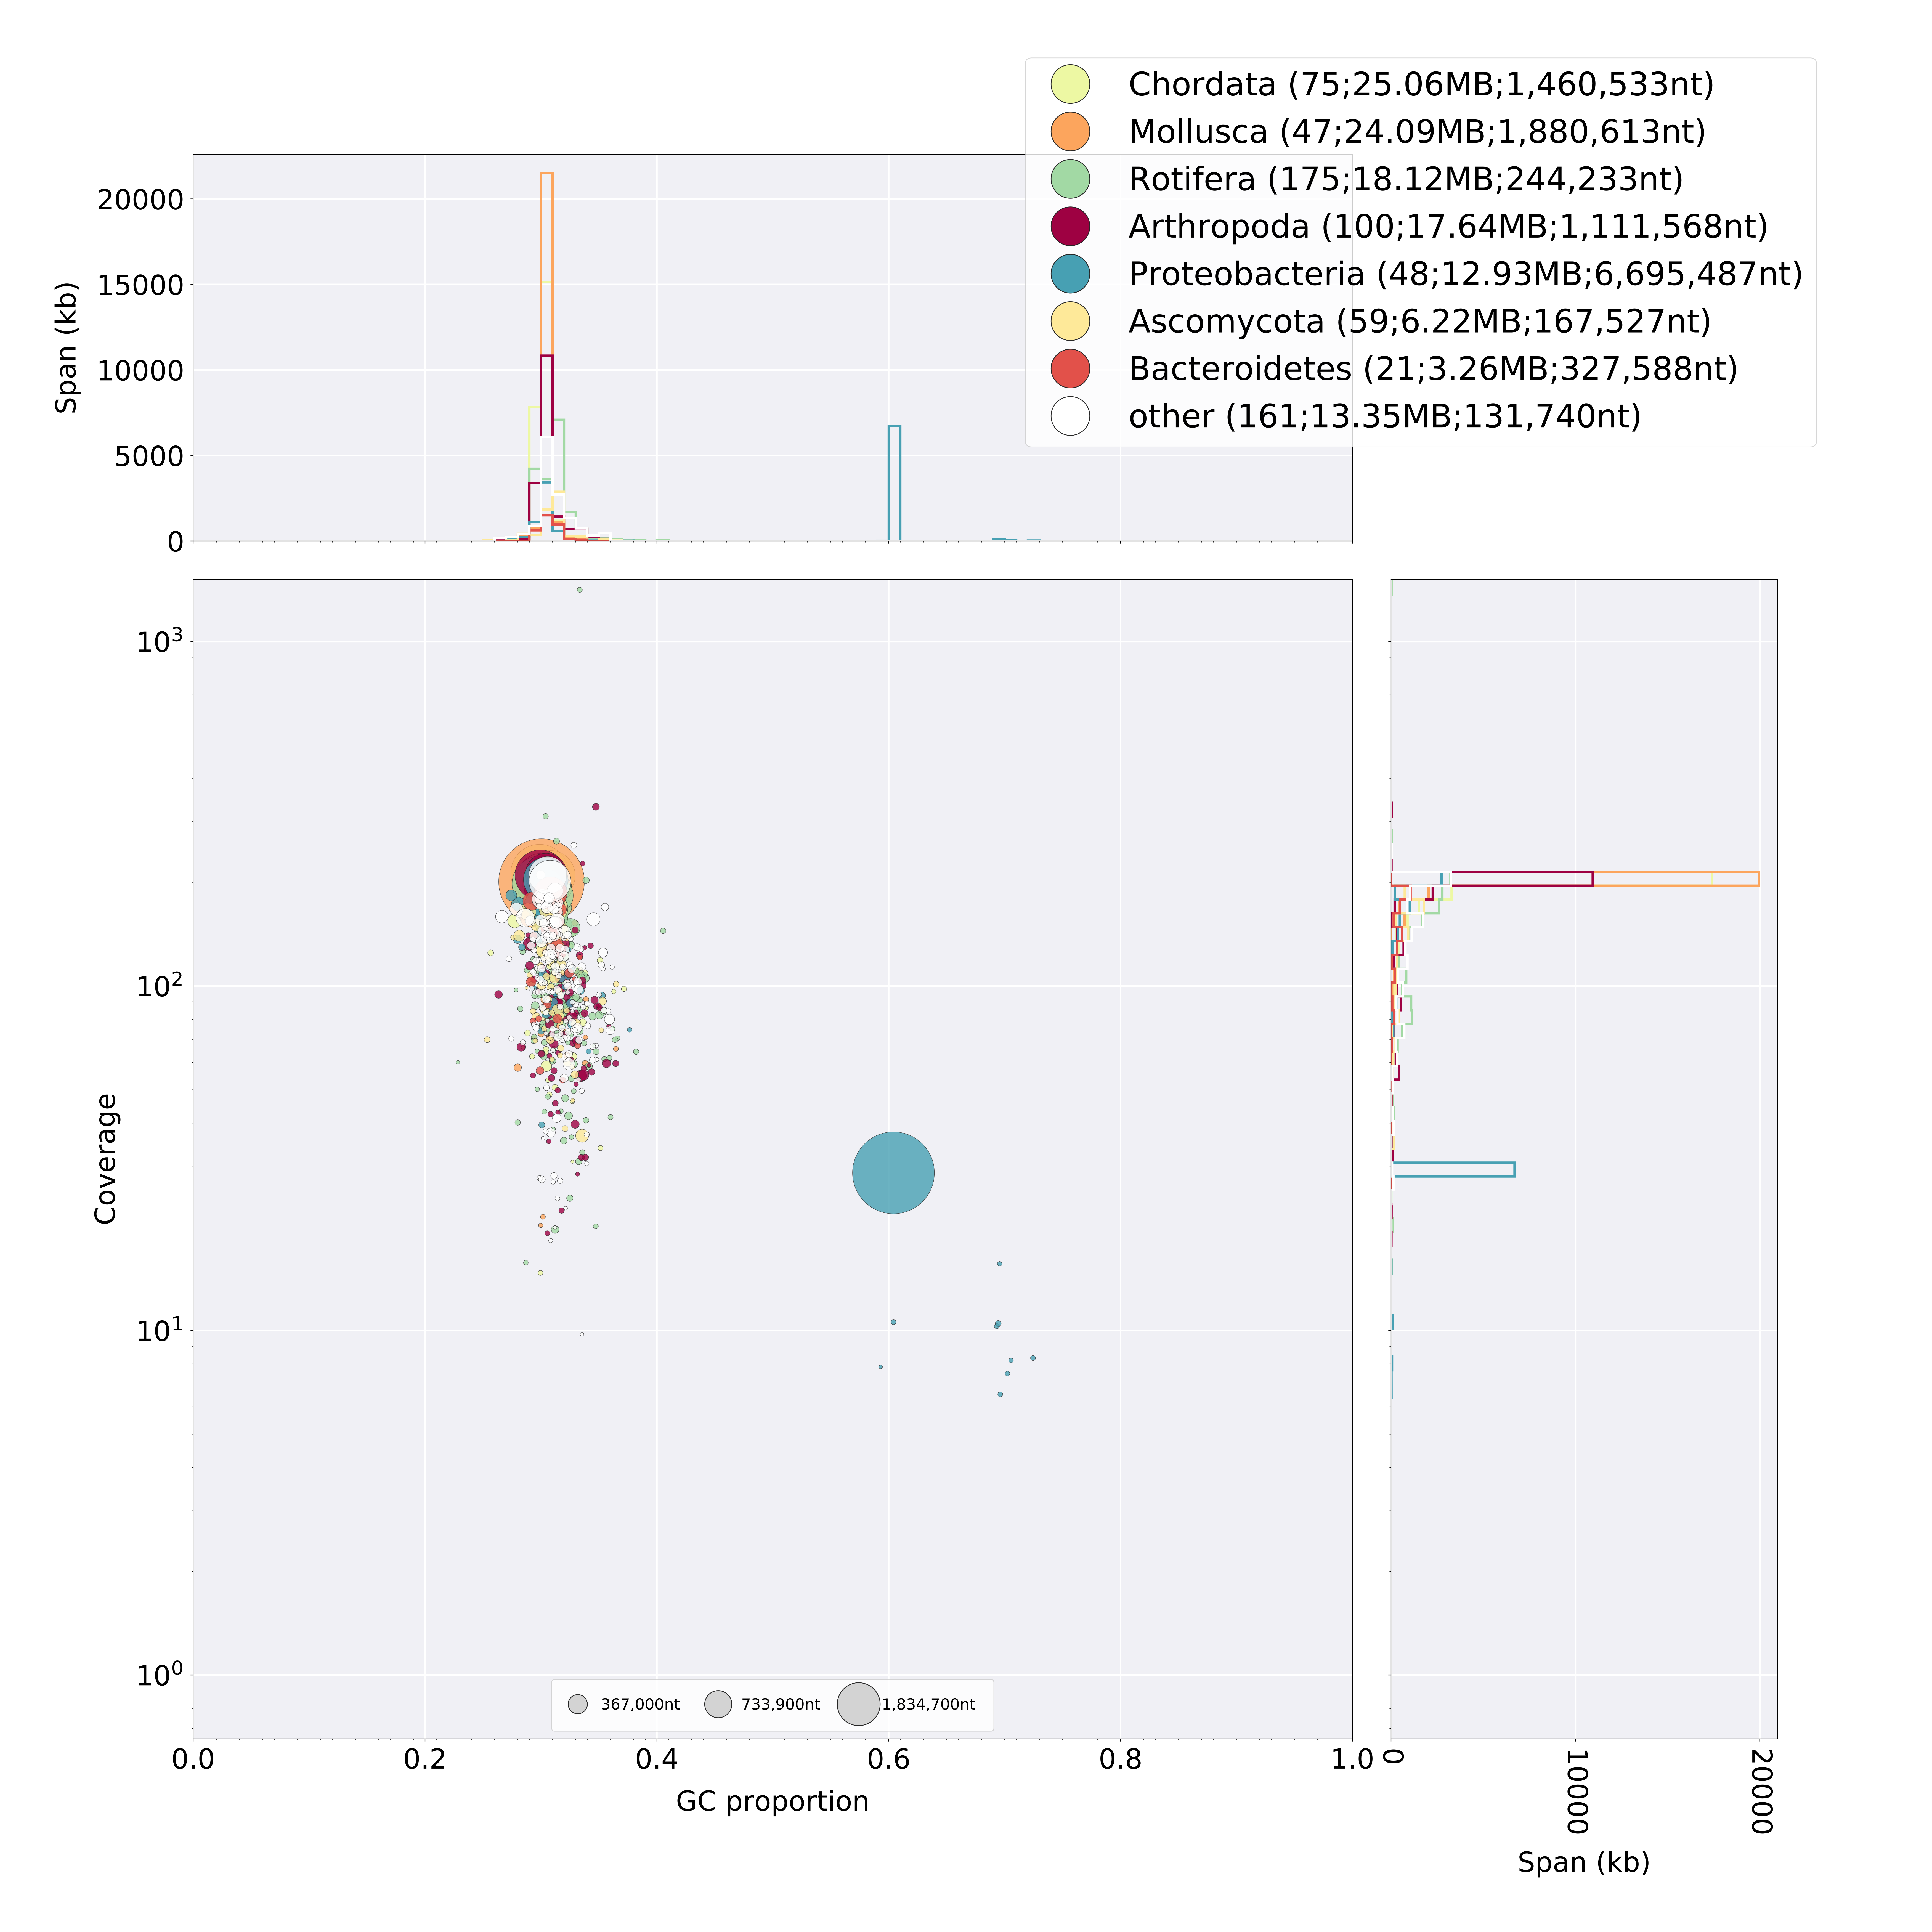
\includegraphics[width=15cm]{fig/benchmark/PB_RA.png}
   \caption{Blobtools v1.0 analysis of a Ra assembly of the full PacBio dataset.}
   \label{fig:blobtools_ra_pb}
 \end{figure}
 
  \begin{figure}[ht]
    \centering
     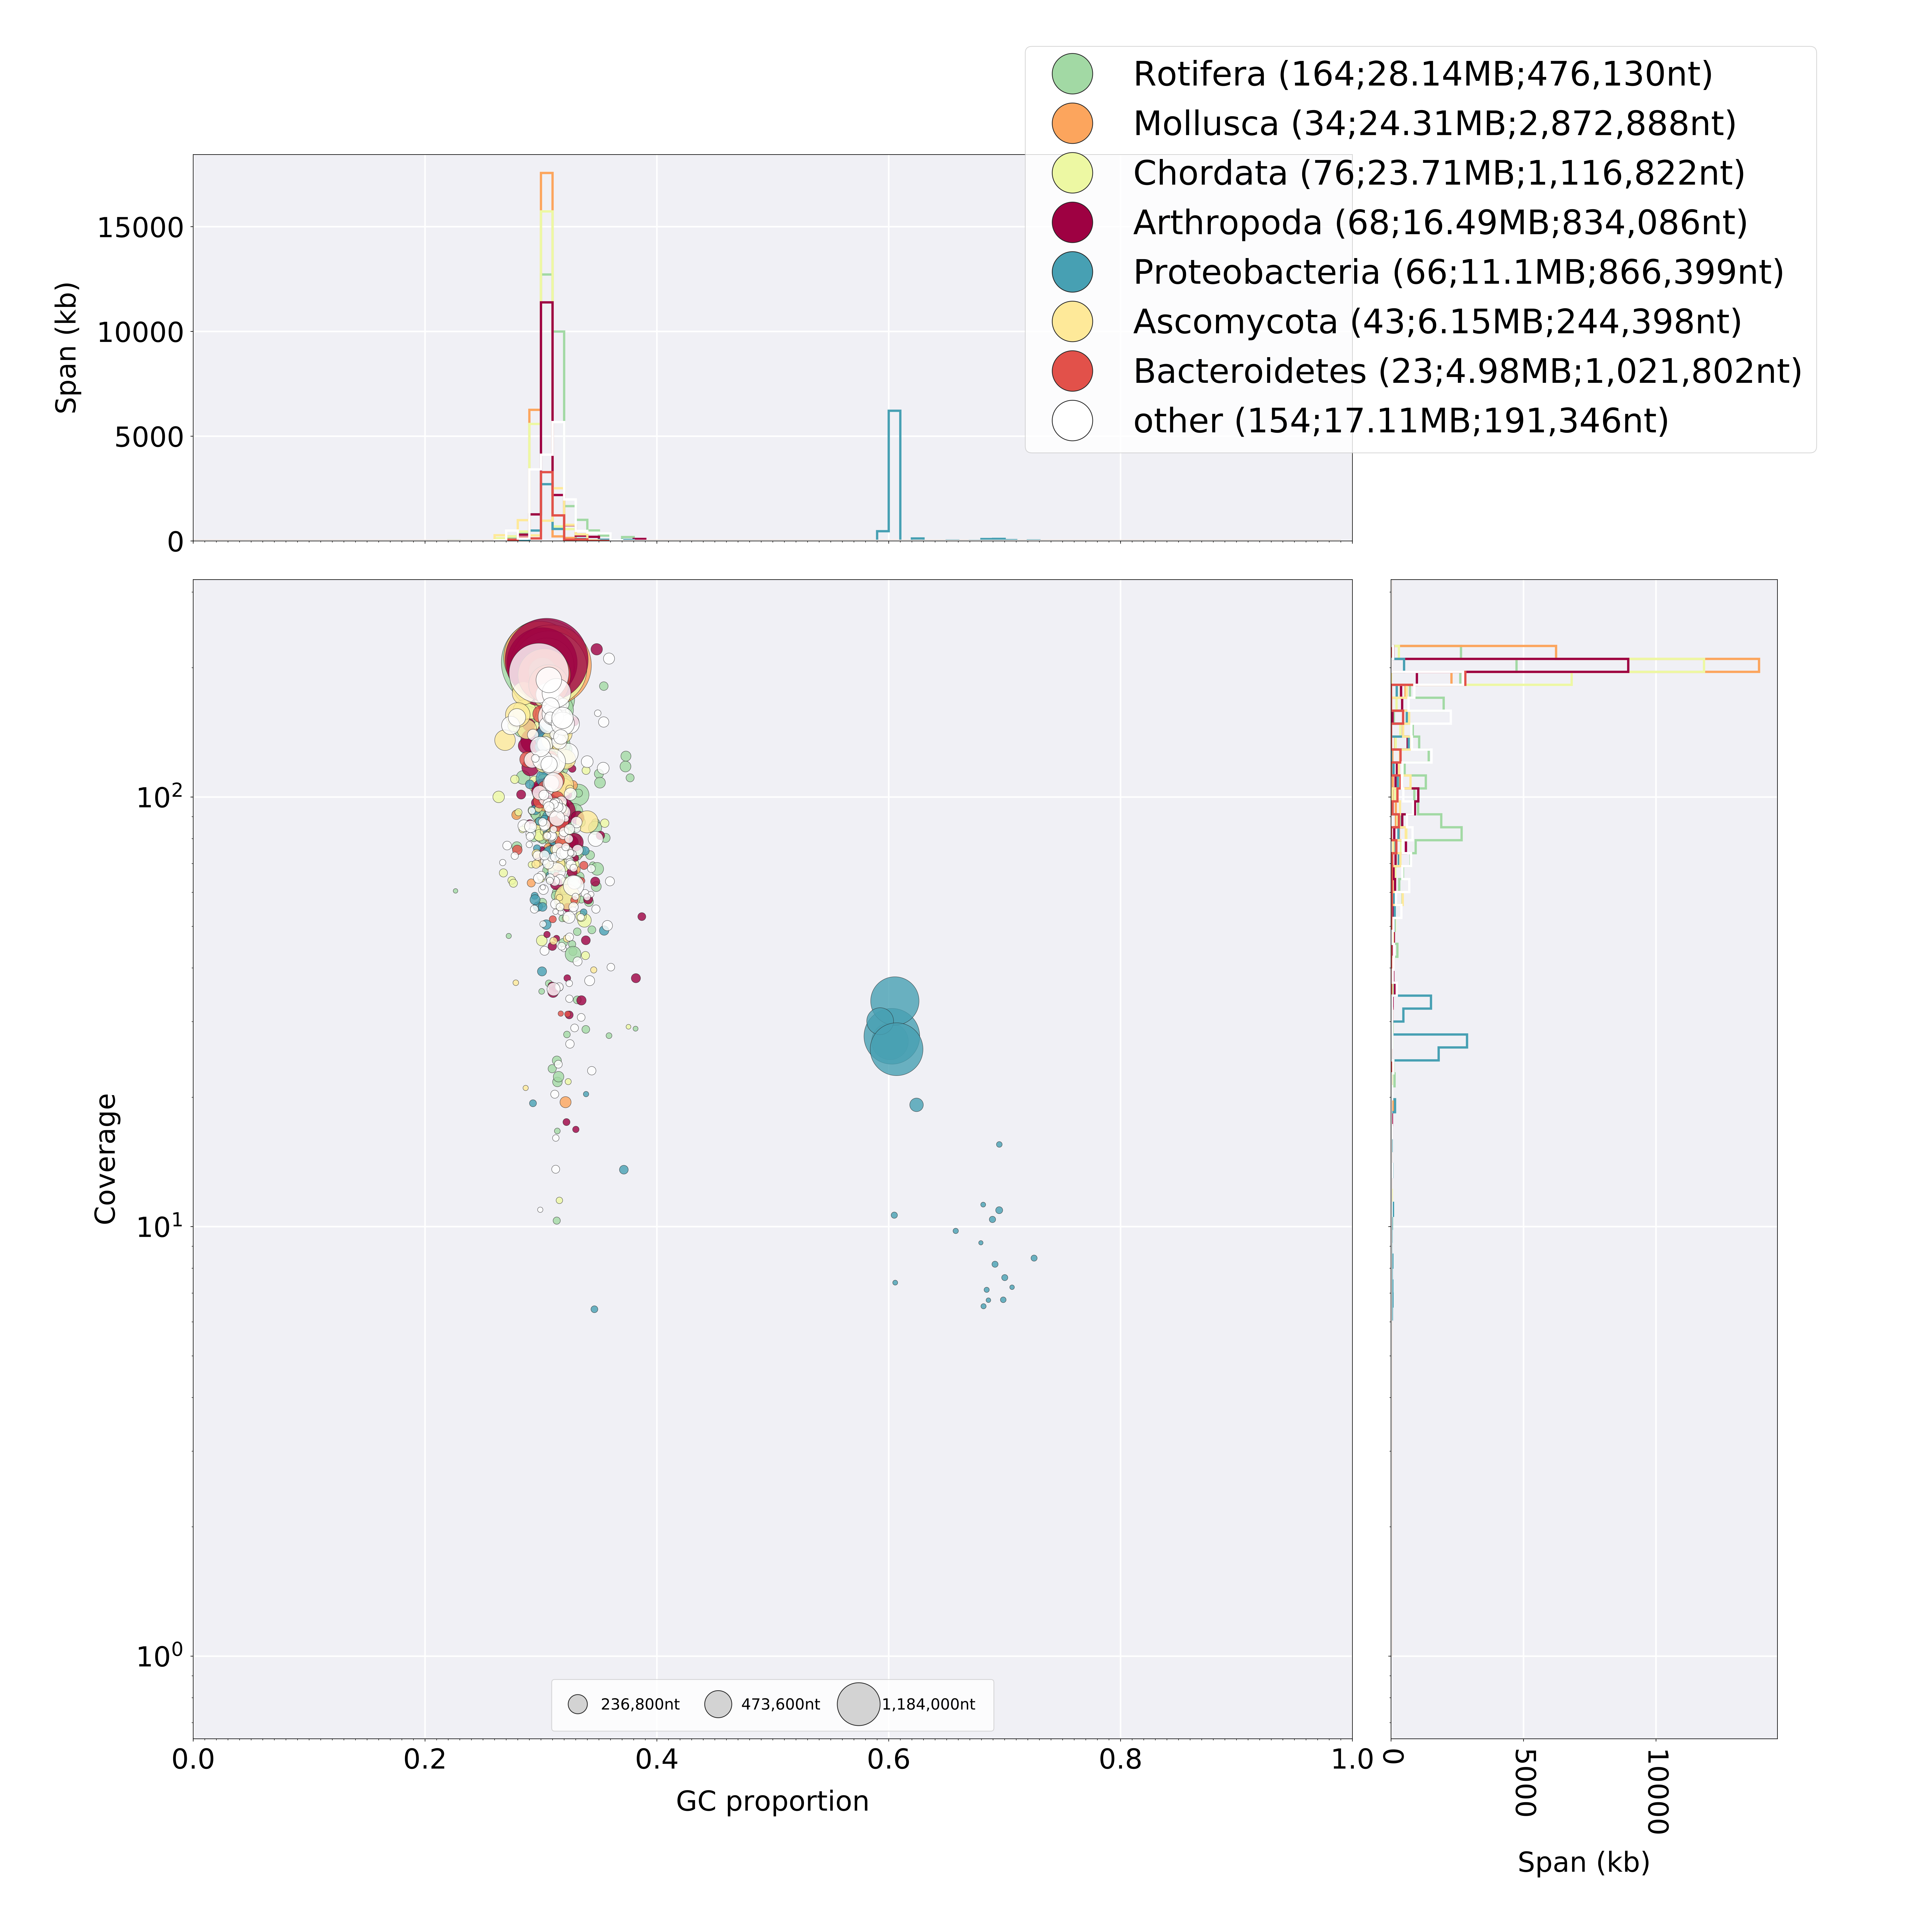
\includegraphics[width=15cm]{fig/benchmark/PB_RAVEN.png}
   \caption{Blobtools v1.0 analysis of a Raven assembly of the full PacBio dataset.}
   \label{fig:blobtools_raven_pb}
 \end{figure}
 
  \begin{figure}[ht]
    \centering
     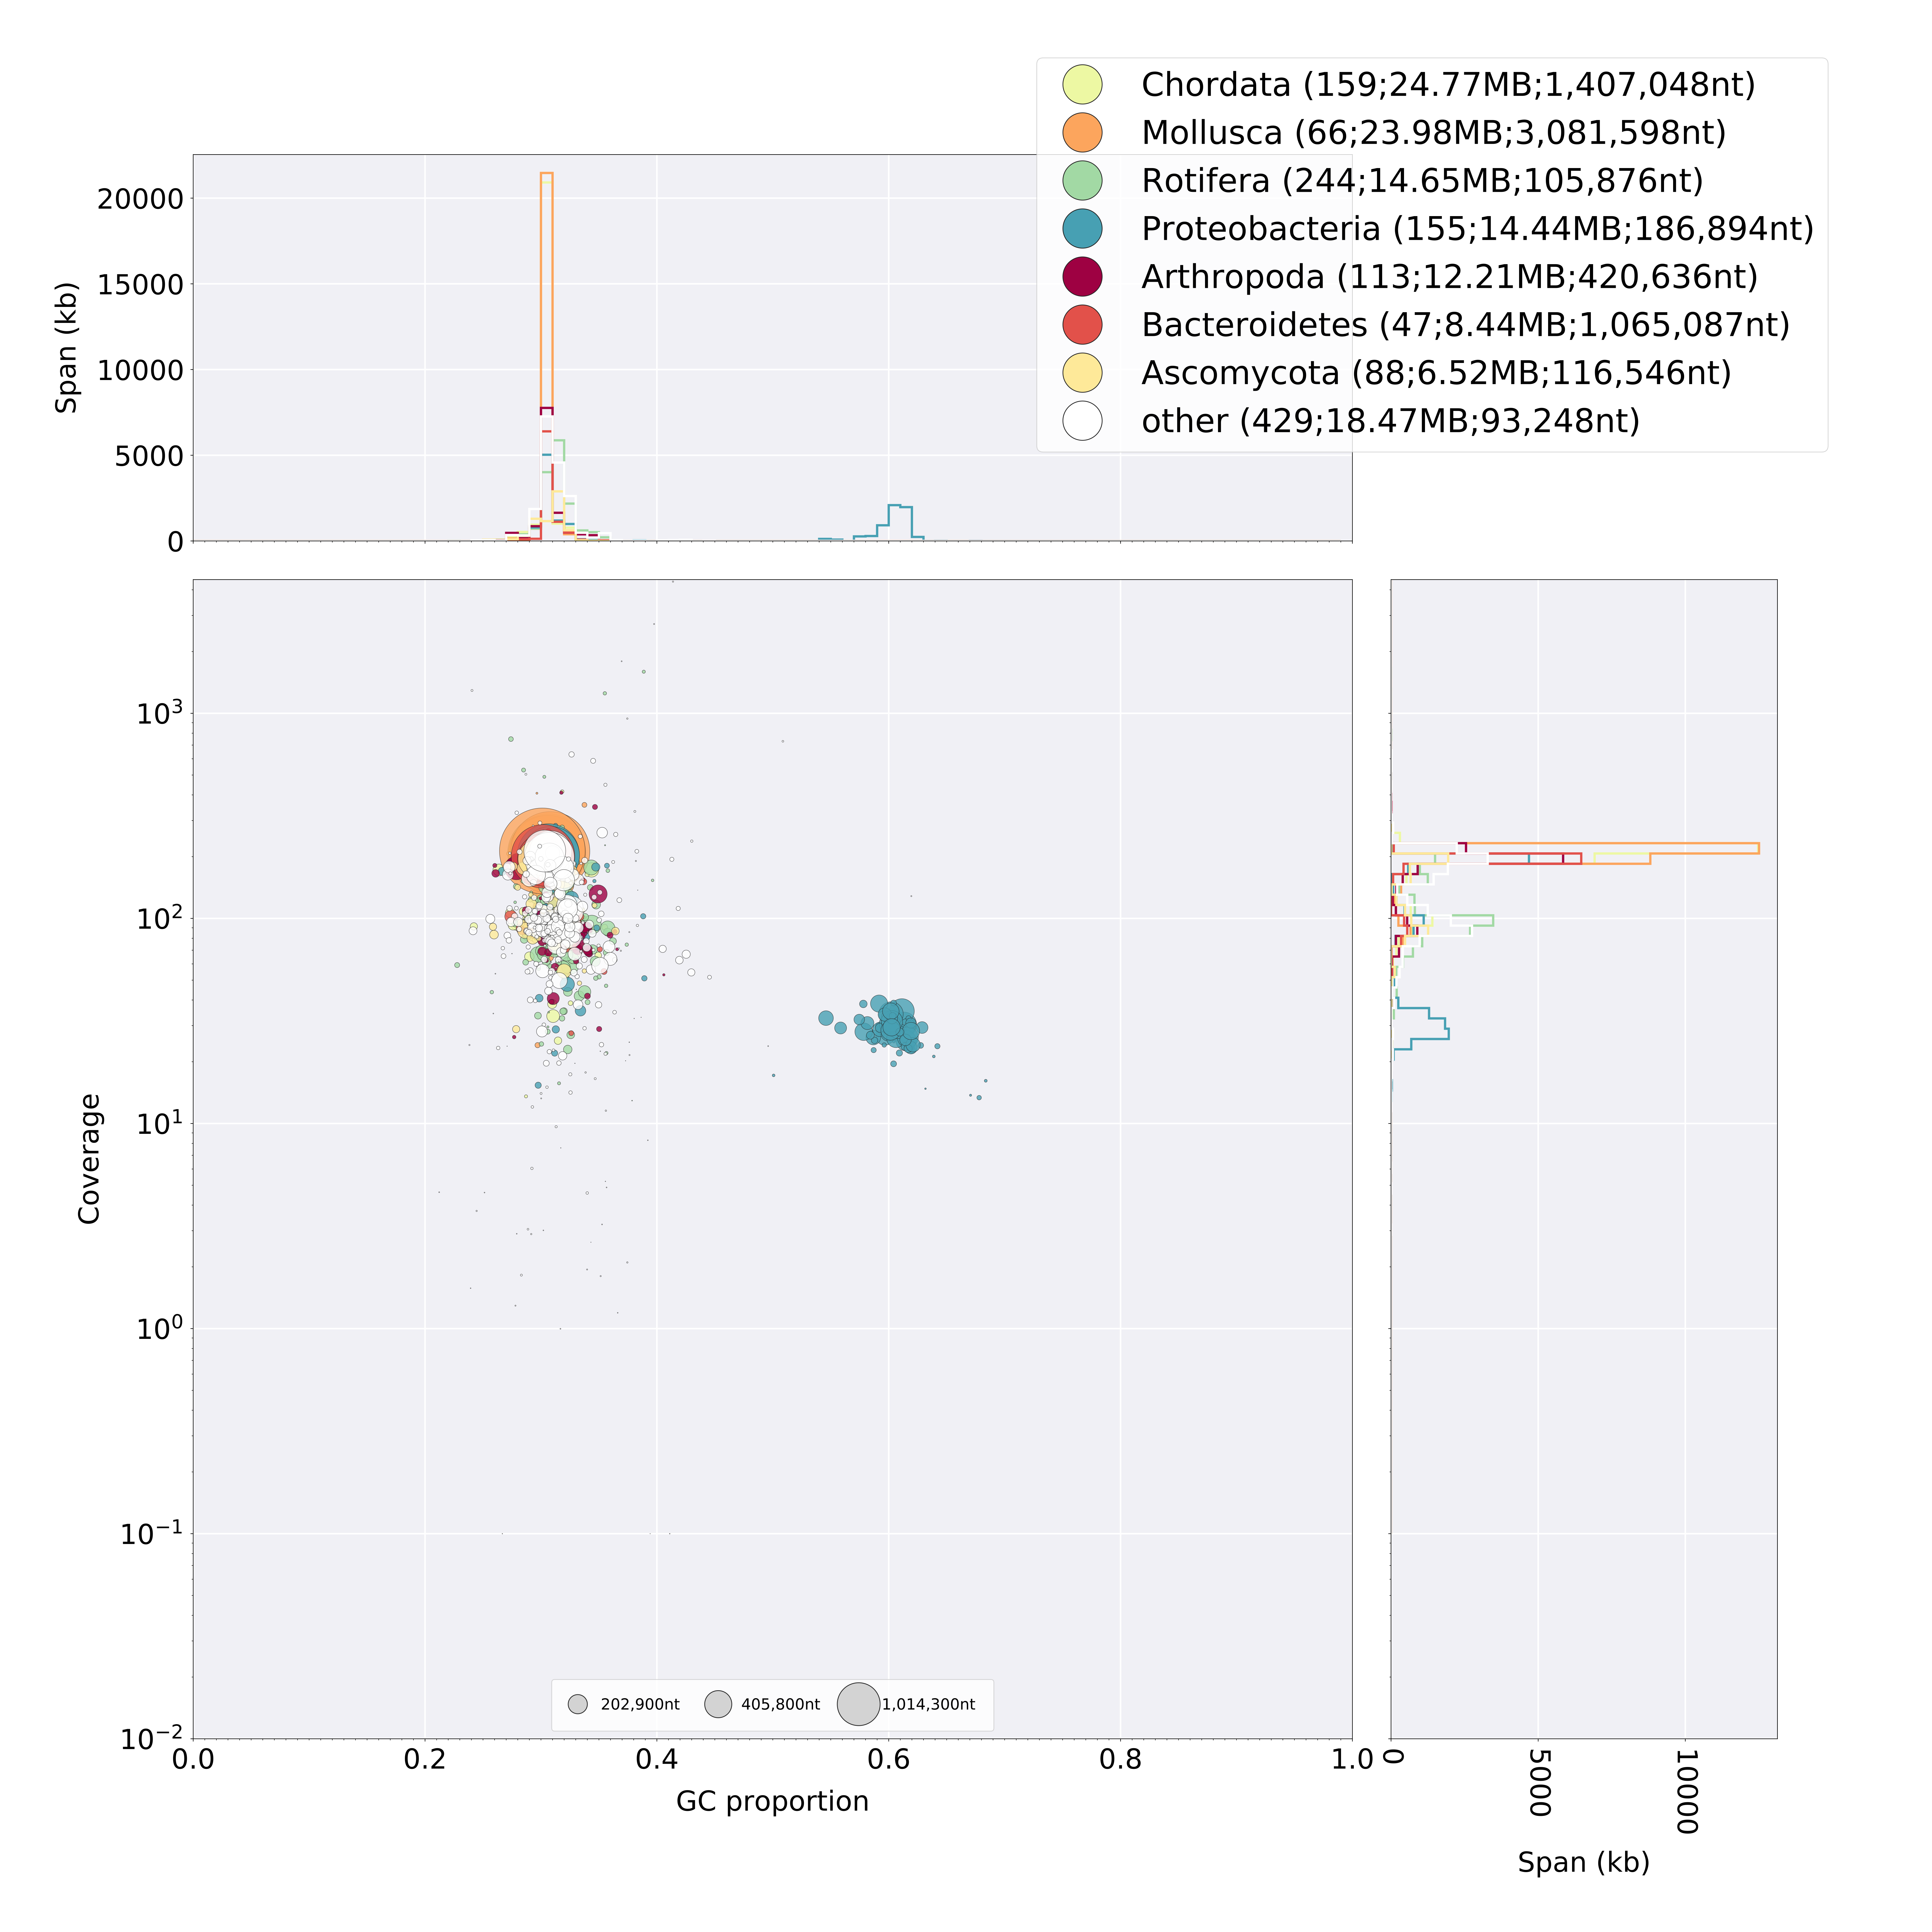
\includegraphics[width=15cm]{fig/benchmark/PB_SHASTA.png}
   \caption{Blobtools v1.0 analysis of a Shasta assembly of the full PacBio dataset.}
   \label{fig:blobtools_shasta_pb}
 \end{figure}

 \begin{figure}[ht]
    \centering
     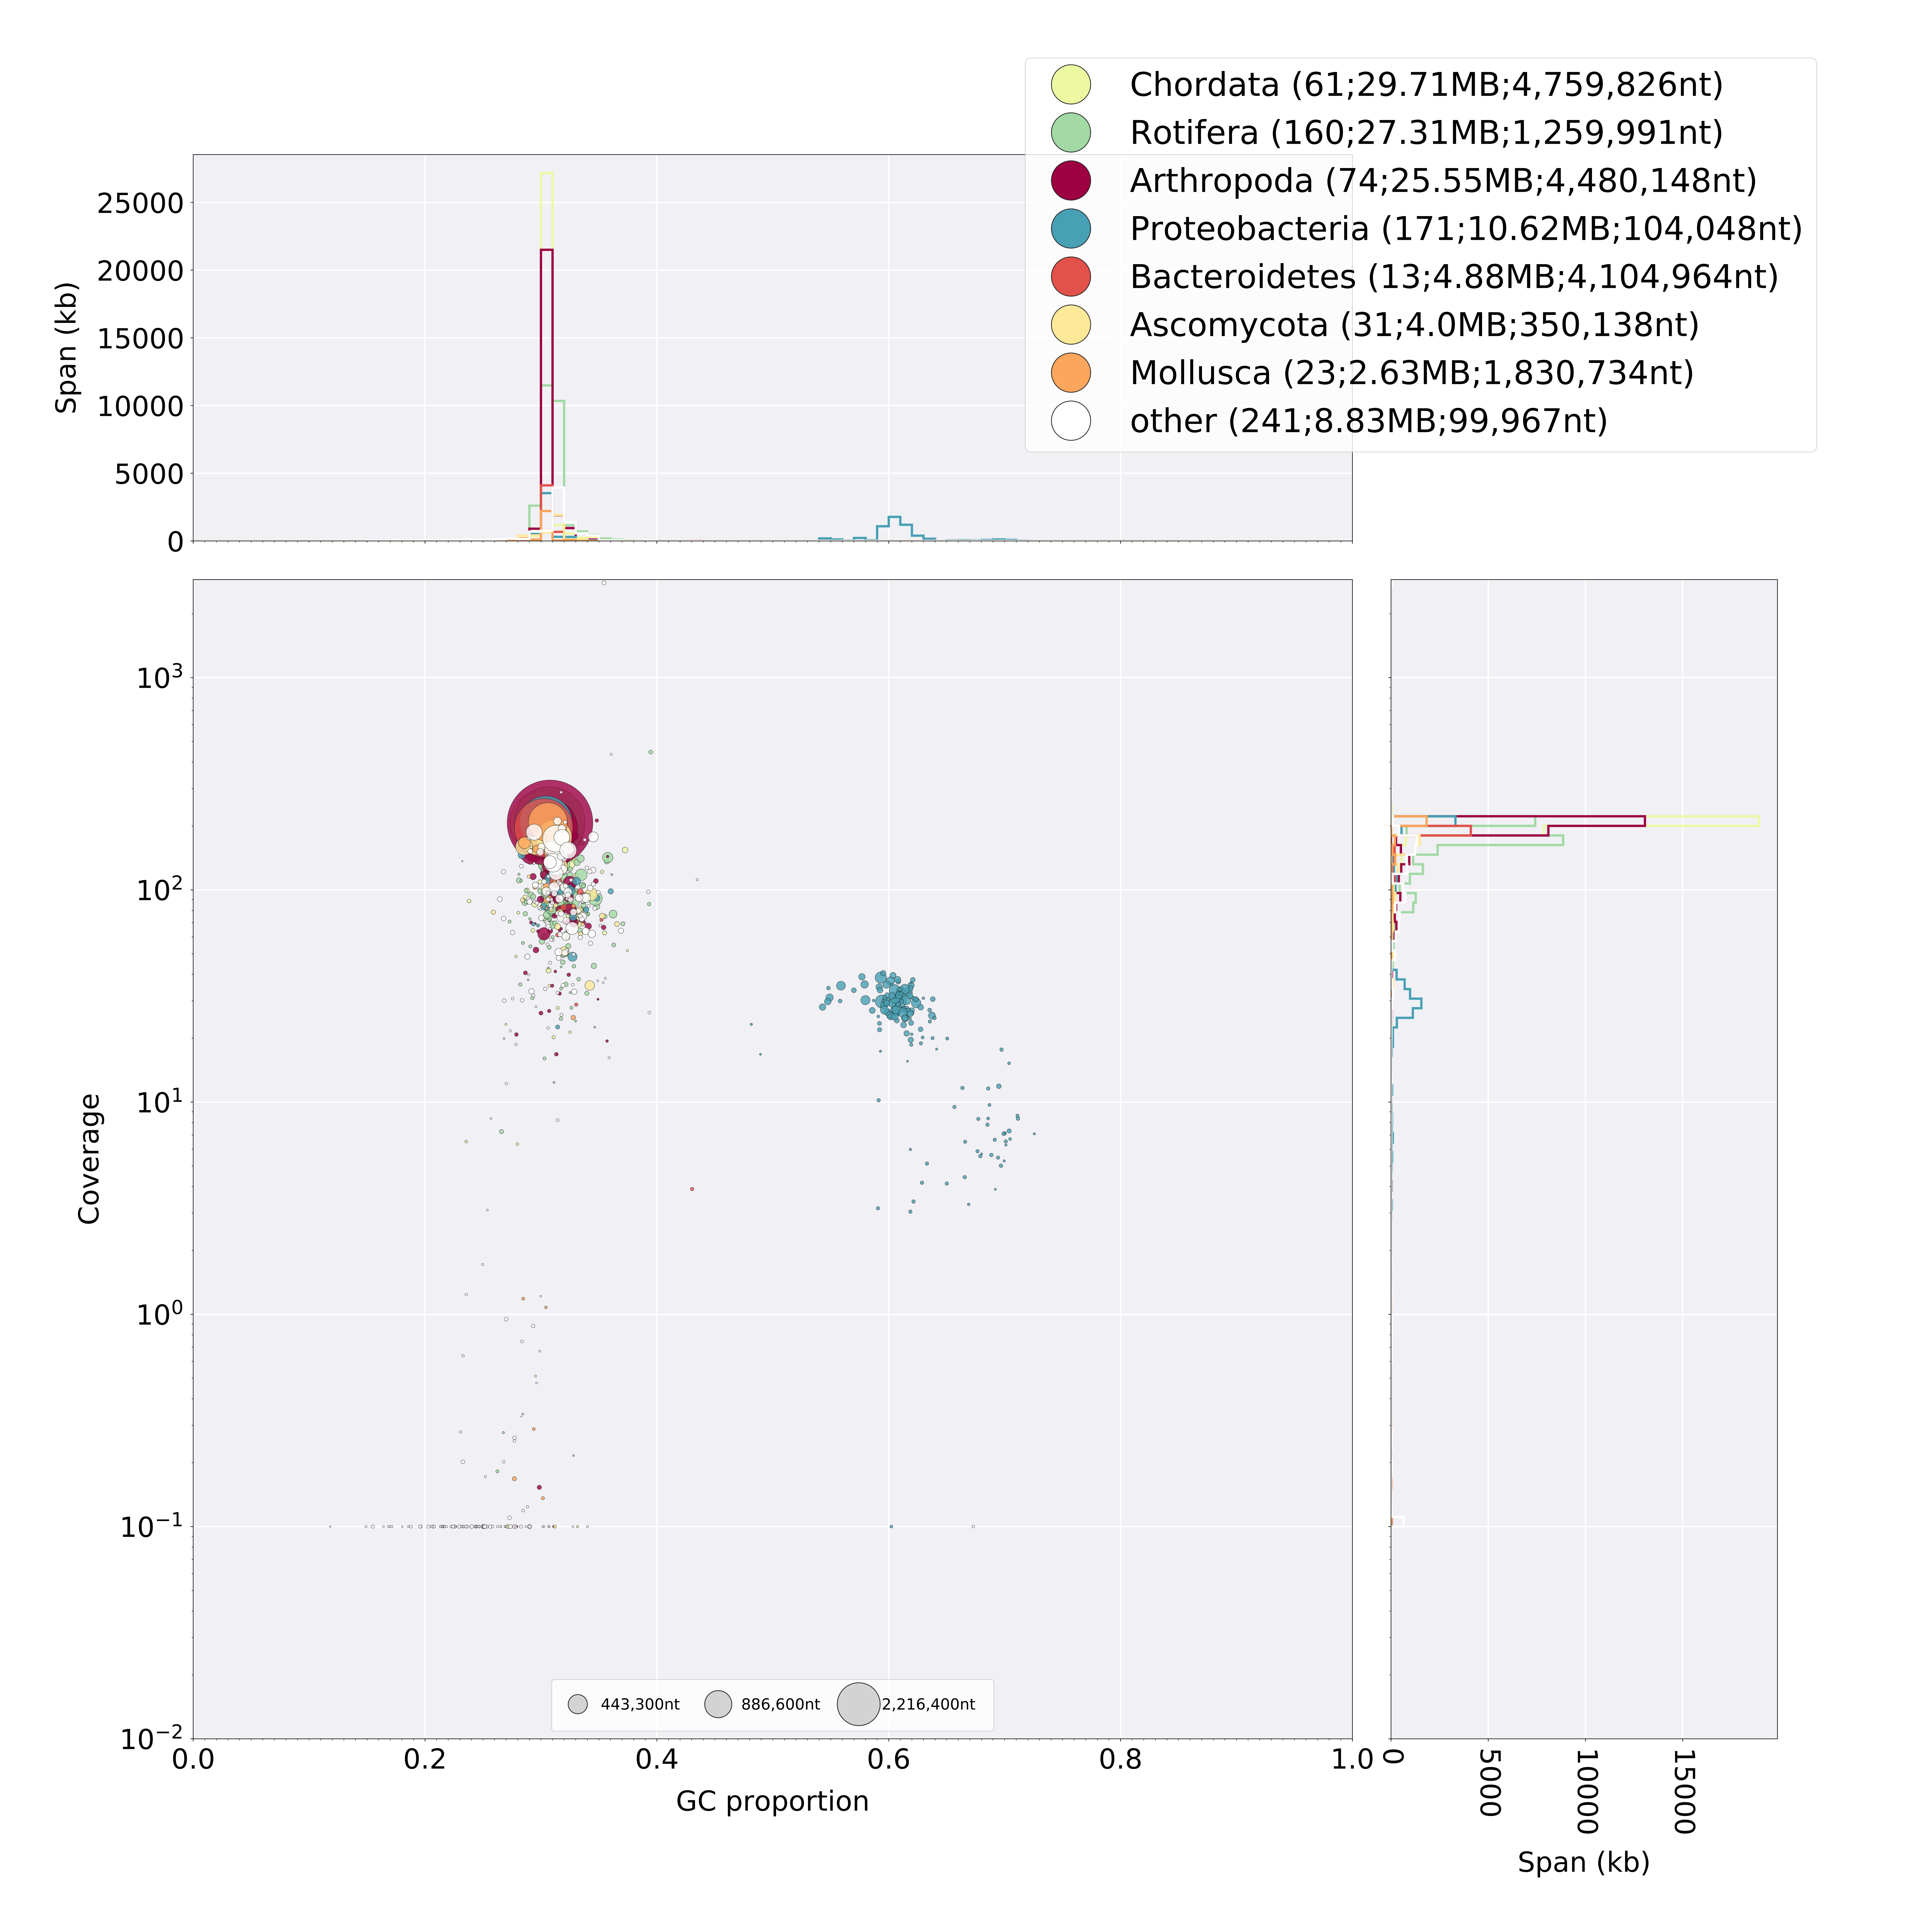
\includegraphics[width=15cm]{fig/benchmark/PB_WTDBG.png}
   \caption{Blobtools v1.0 analysis of a wtdbg2 assembly of the full PacBio dataset.}
   \label{fig:blobtools_wtdbg2_pb}
 \end{figure}

    \begin{figure}[ht]
    \centering
     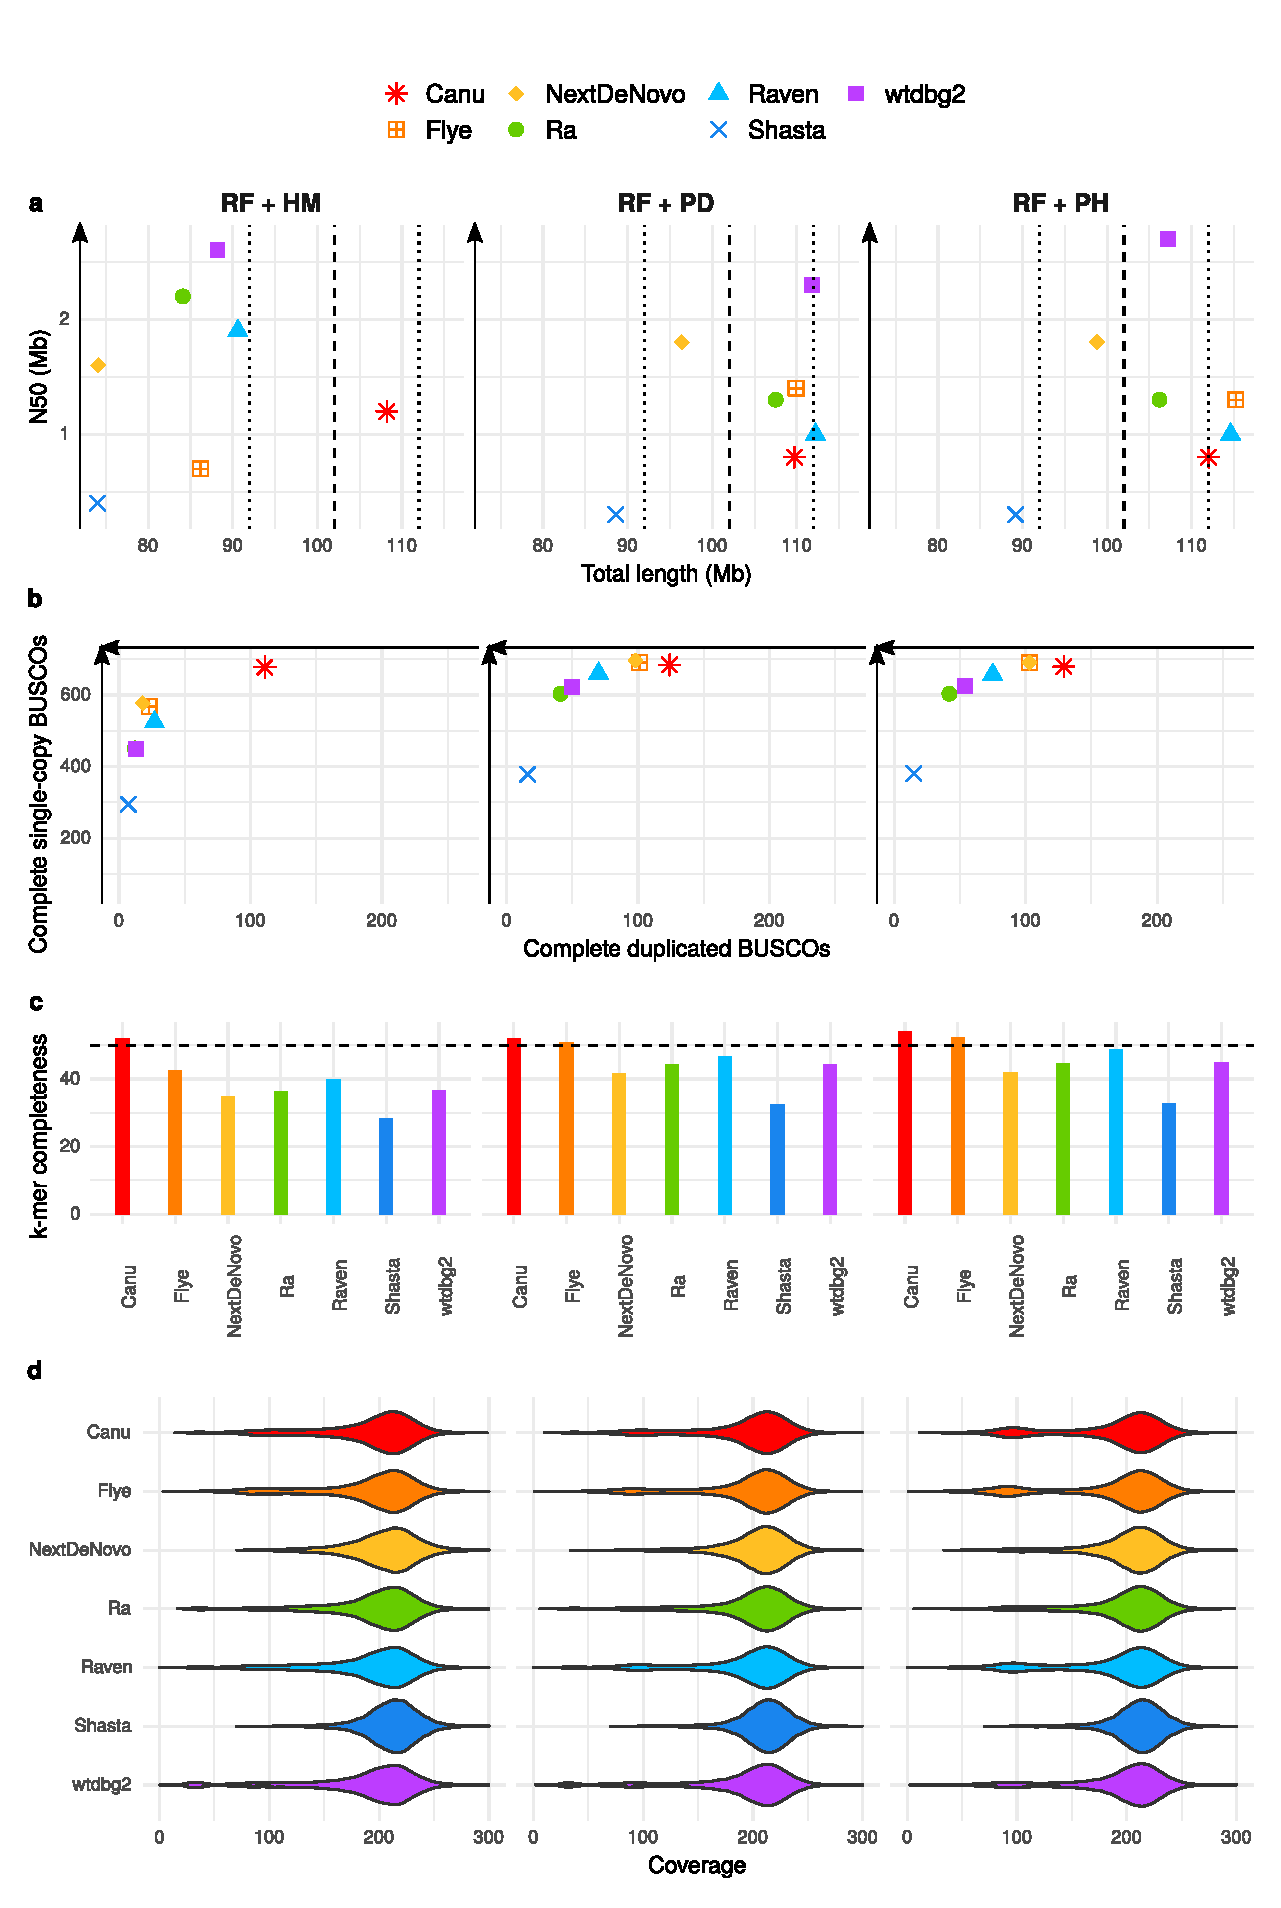
\includegraphics[width=13.5cm]{fig/benchmark/supp_pacbio_filtering_purging_v20201012.eps}
   \caption{Statistics of PacBio assemblies obtained from the filtered PacBio dataset of reads longer than 15 kb, with a subsequent removal of uncollapsed haplotypes with HaploMerger2 (HM), purge\_dups (PD), or purge\_haplotigs (PH). a) N50 plotted against total assembly length. The dashed line indicates the expected genome size, with a +/- 10 Mb margin delimited by the dotted lines. b) Number of complete single-copy BUSCOs plotted against number of complete duplicated BUSCOs, from a total of 954 orthologs. c) \textit{k}-mer completeness. The dashed line indicates the expected 50\% completeness. d) Long-read coverage distribution over the contigs.}
   \label{fig:pacbio_filtering_purging}
 \end{figure}
 
     \begin{figure}[ht]
    \centering
     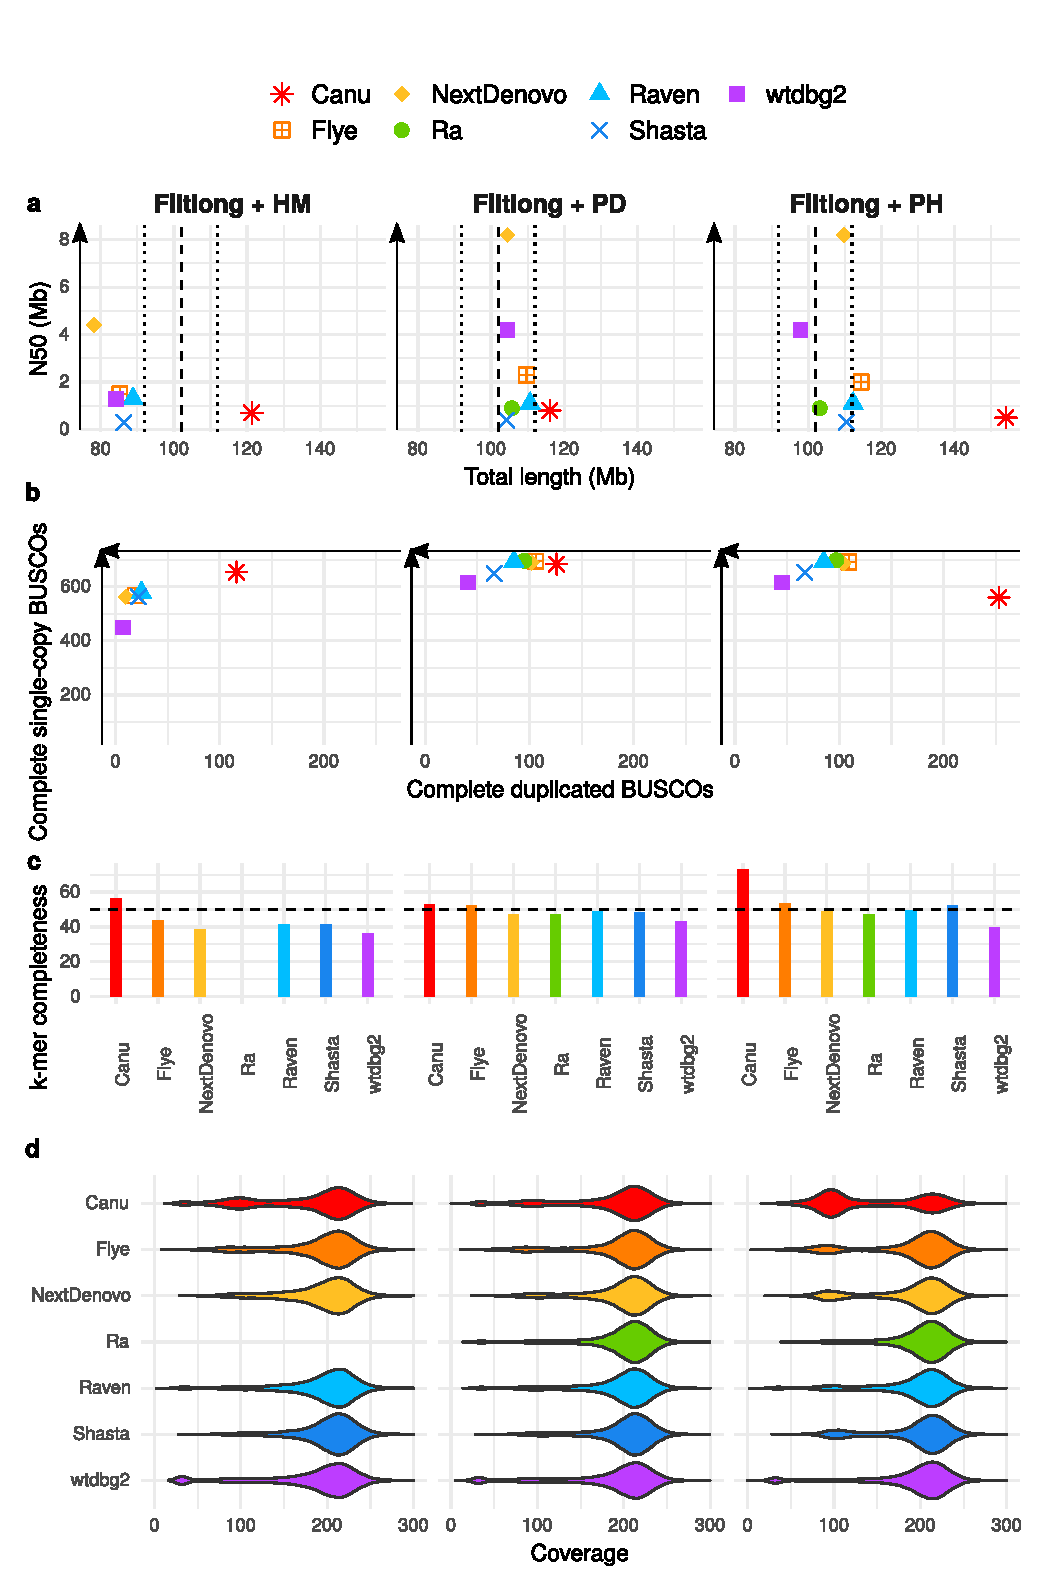
\includegraphics[width=13.5cm]{fig/benchmark/supp_pacbio_filtlong_purging.eps}
   \caption{Statistics of PacBio assemblies obtained from the PacBio dataset filtered with Filtlong, with a subsequent removal of uncollapsed haplotypes with HaploMerger2 (HM), purge\_dups (PD), or purge\_haplotigs (PH). a) N50 plotted against total assembly length. The dashed line indicates the expected genome size, with a +/- 10 Mb margin delimited by the dotted lines. b) Number of complete single-copy BUSCOs plotted against number of complete duplicated BUSCOs, from a total of 954 orthologs. c) \textit{k}-mer completeness. The dashed line indicates the expected 50\% completeness. d) Long-read coverage distribution over the contigs.}
   \label{fig:pacbio_filtlong_purging}
 \end{figure}
 
   \begin{figure}[ht]
    \centering
     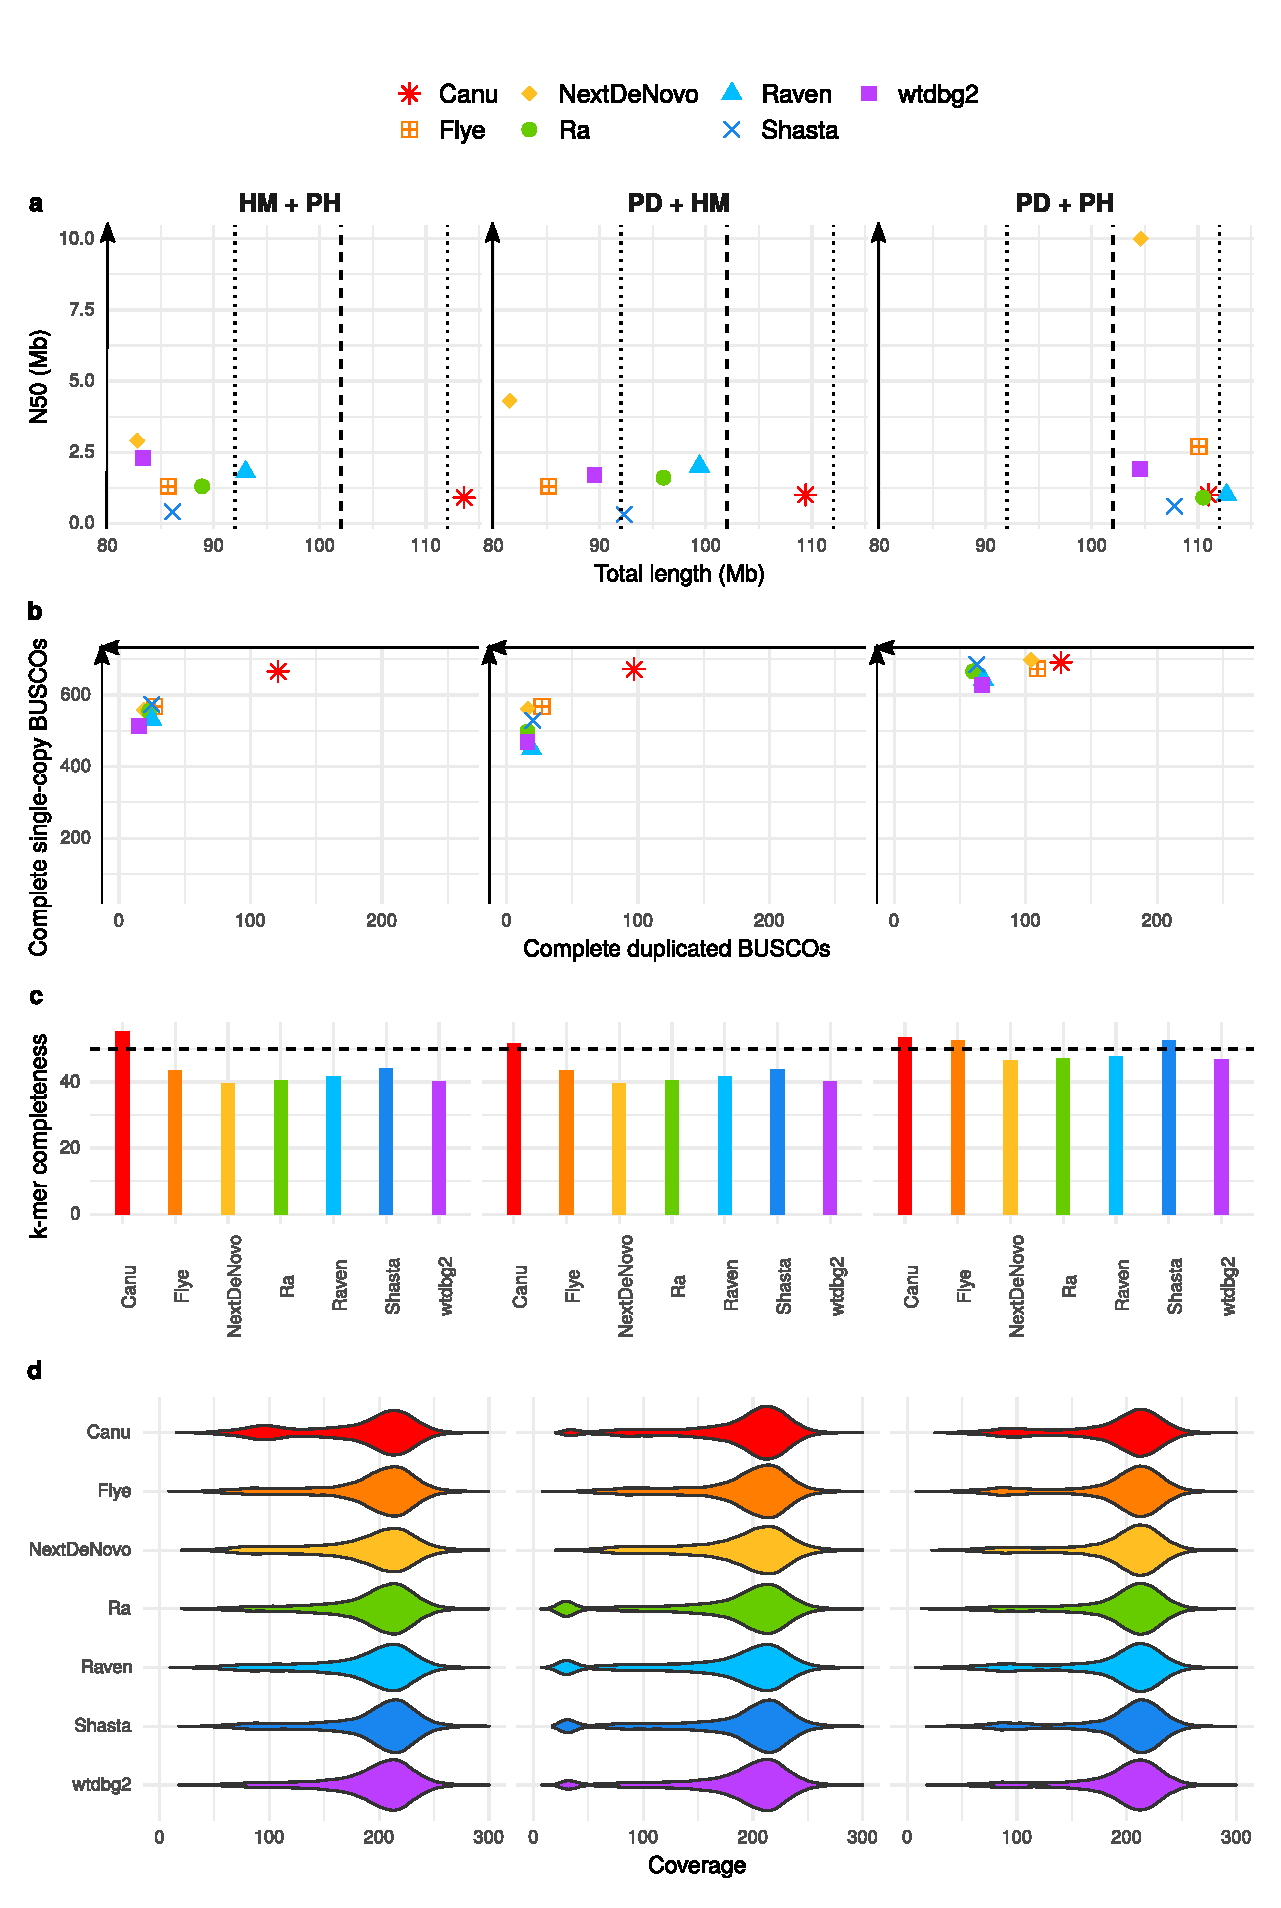
\includegraphics[width=13.5cm]{fig/benchmark/supp_pacbio_purging_combinations_v20200919.eps}
   \caption{Statistics of PacBio assemblies obtained from the full PacBio dataset with a subsequent removal of uncollapsed haplotypes with combinations of HaploMerger2 (HM), purge\_dups (PD), and purge\_haplotigs (PH). a) N50 plotted against total assembly length. The dashed line indicates the expected genome size, with a +/- 10 Mb margin delimited by the dotted lines. b) Number of complete single-copy BUSCOs plotted against number of complete duplicated BUSCOs, from a total of 954 orthologs. c) \textit{k}-mer completeness. The dashed line indicates the expected 50\% completeness. d) Long-read coverage distribution over the contigs.}
   \label{fig:pacbio_purging_combinations}
 \end{figure}
 
 
 \begin{figure}[ht]
    \centering
     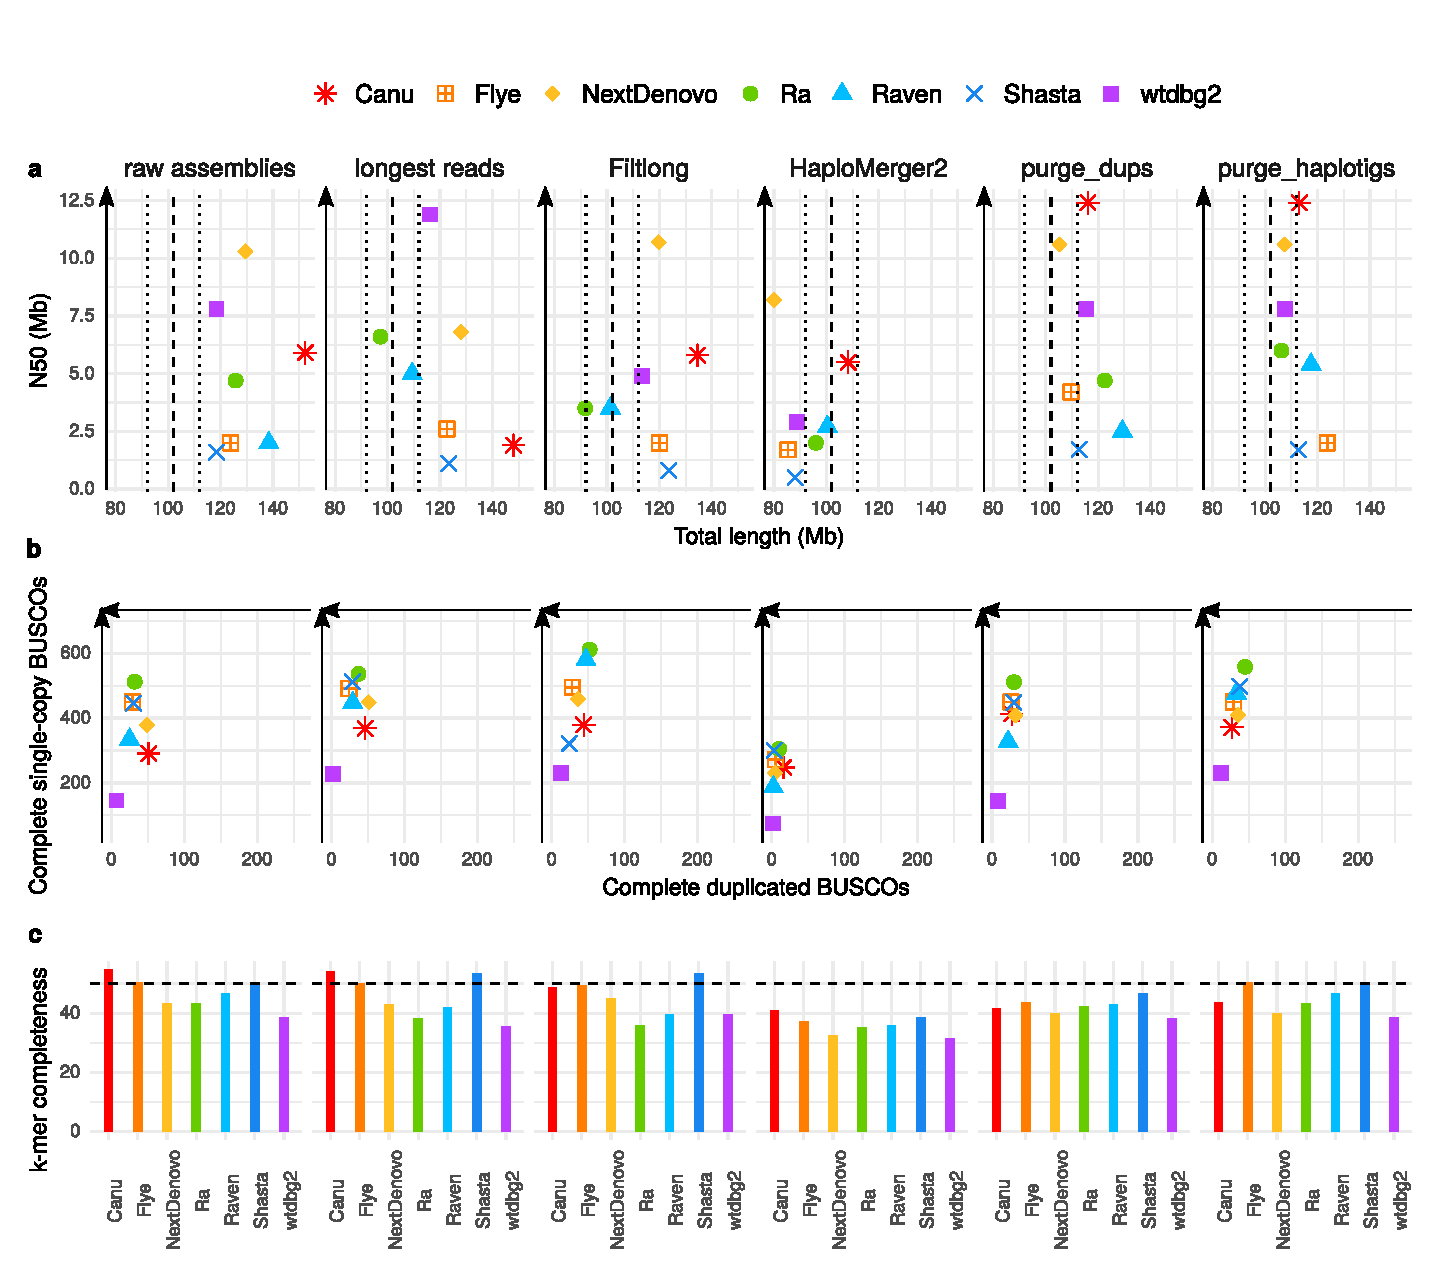
\includegraphics[width=13.5cm]{fig/benchmark/nanopore_all_v20210317.eps}
   \caption{Statistics of raw assemblies obtained from the full Nanopore dataset (raw assemblies), with a preliminary read filtering step (keeping only reads larger than 30 kb, or those selected by Filtlong based on quality and length) or a subsequent removal of uncollapsed haplotypes with HaploMerger2, purge\_dups, or purge\_haplotigs. a) N50 plotted against total assembly length. The dashed line indicates the expected genome size, with +/- 10 Mb margin delimited by the dotted lines. b) Number of complete single-copy BUSCOs plotted against number of complete duplicated BUSCOs, from a total of 954 orthologs. c) \textit{k}-mer completeness. The dashed line indicates the expected 50\% completeness.}
   \label{fig:nanopore_full_stats}
 \end{figure}
 
   \begin{figure}[ht]
    \centering
     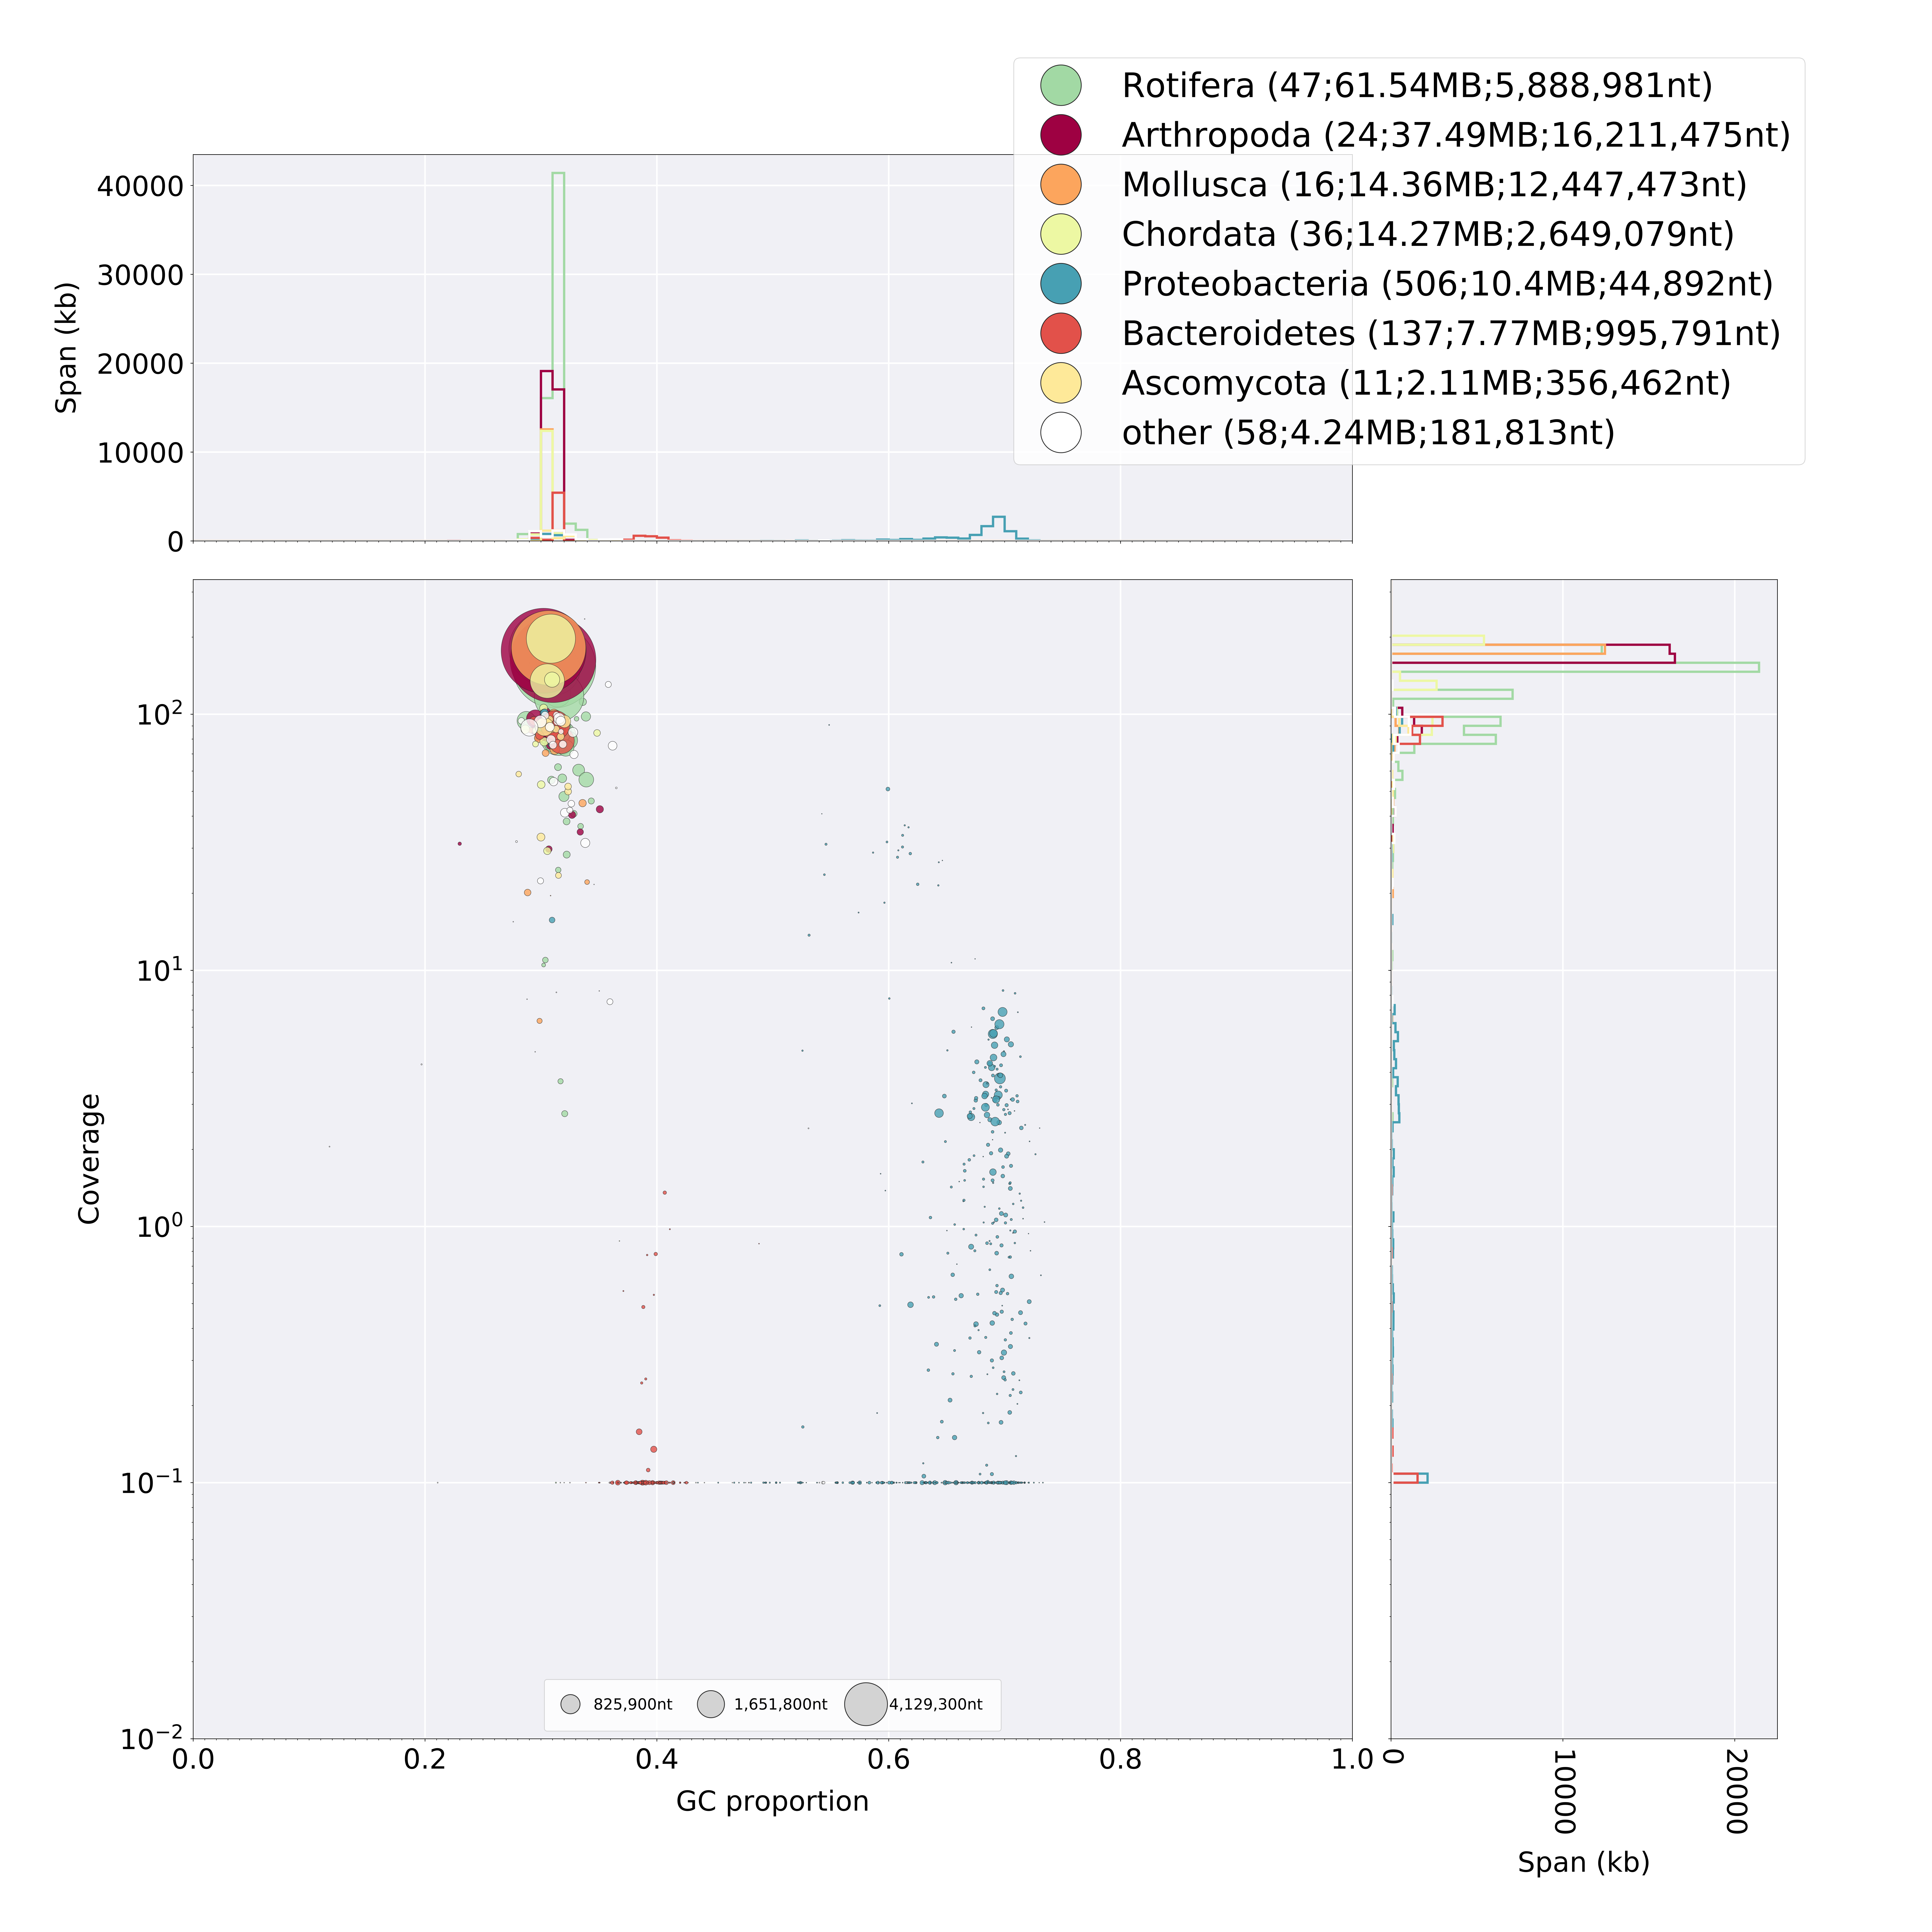
\includegraphics[width=15cm]{fig/benchmark/ONT_CANU.png}
   \caption{Blobtools v1.0 analysis of a Canu assembly of the full Nanopore dataset.}
   \label{fig:blobtools_canu_ont}
 \end{figure}
 
   \begin{figure}[ht]
    \centering
     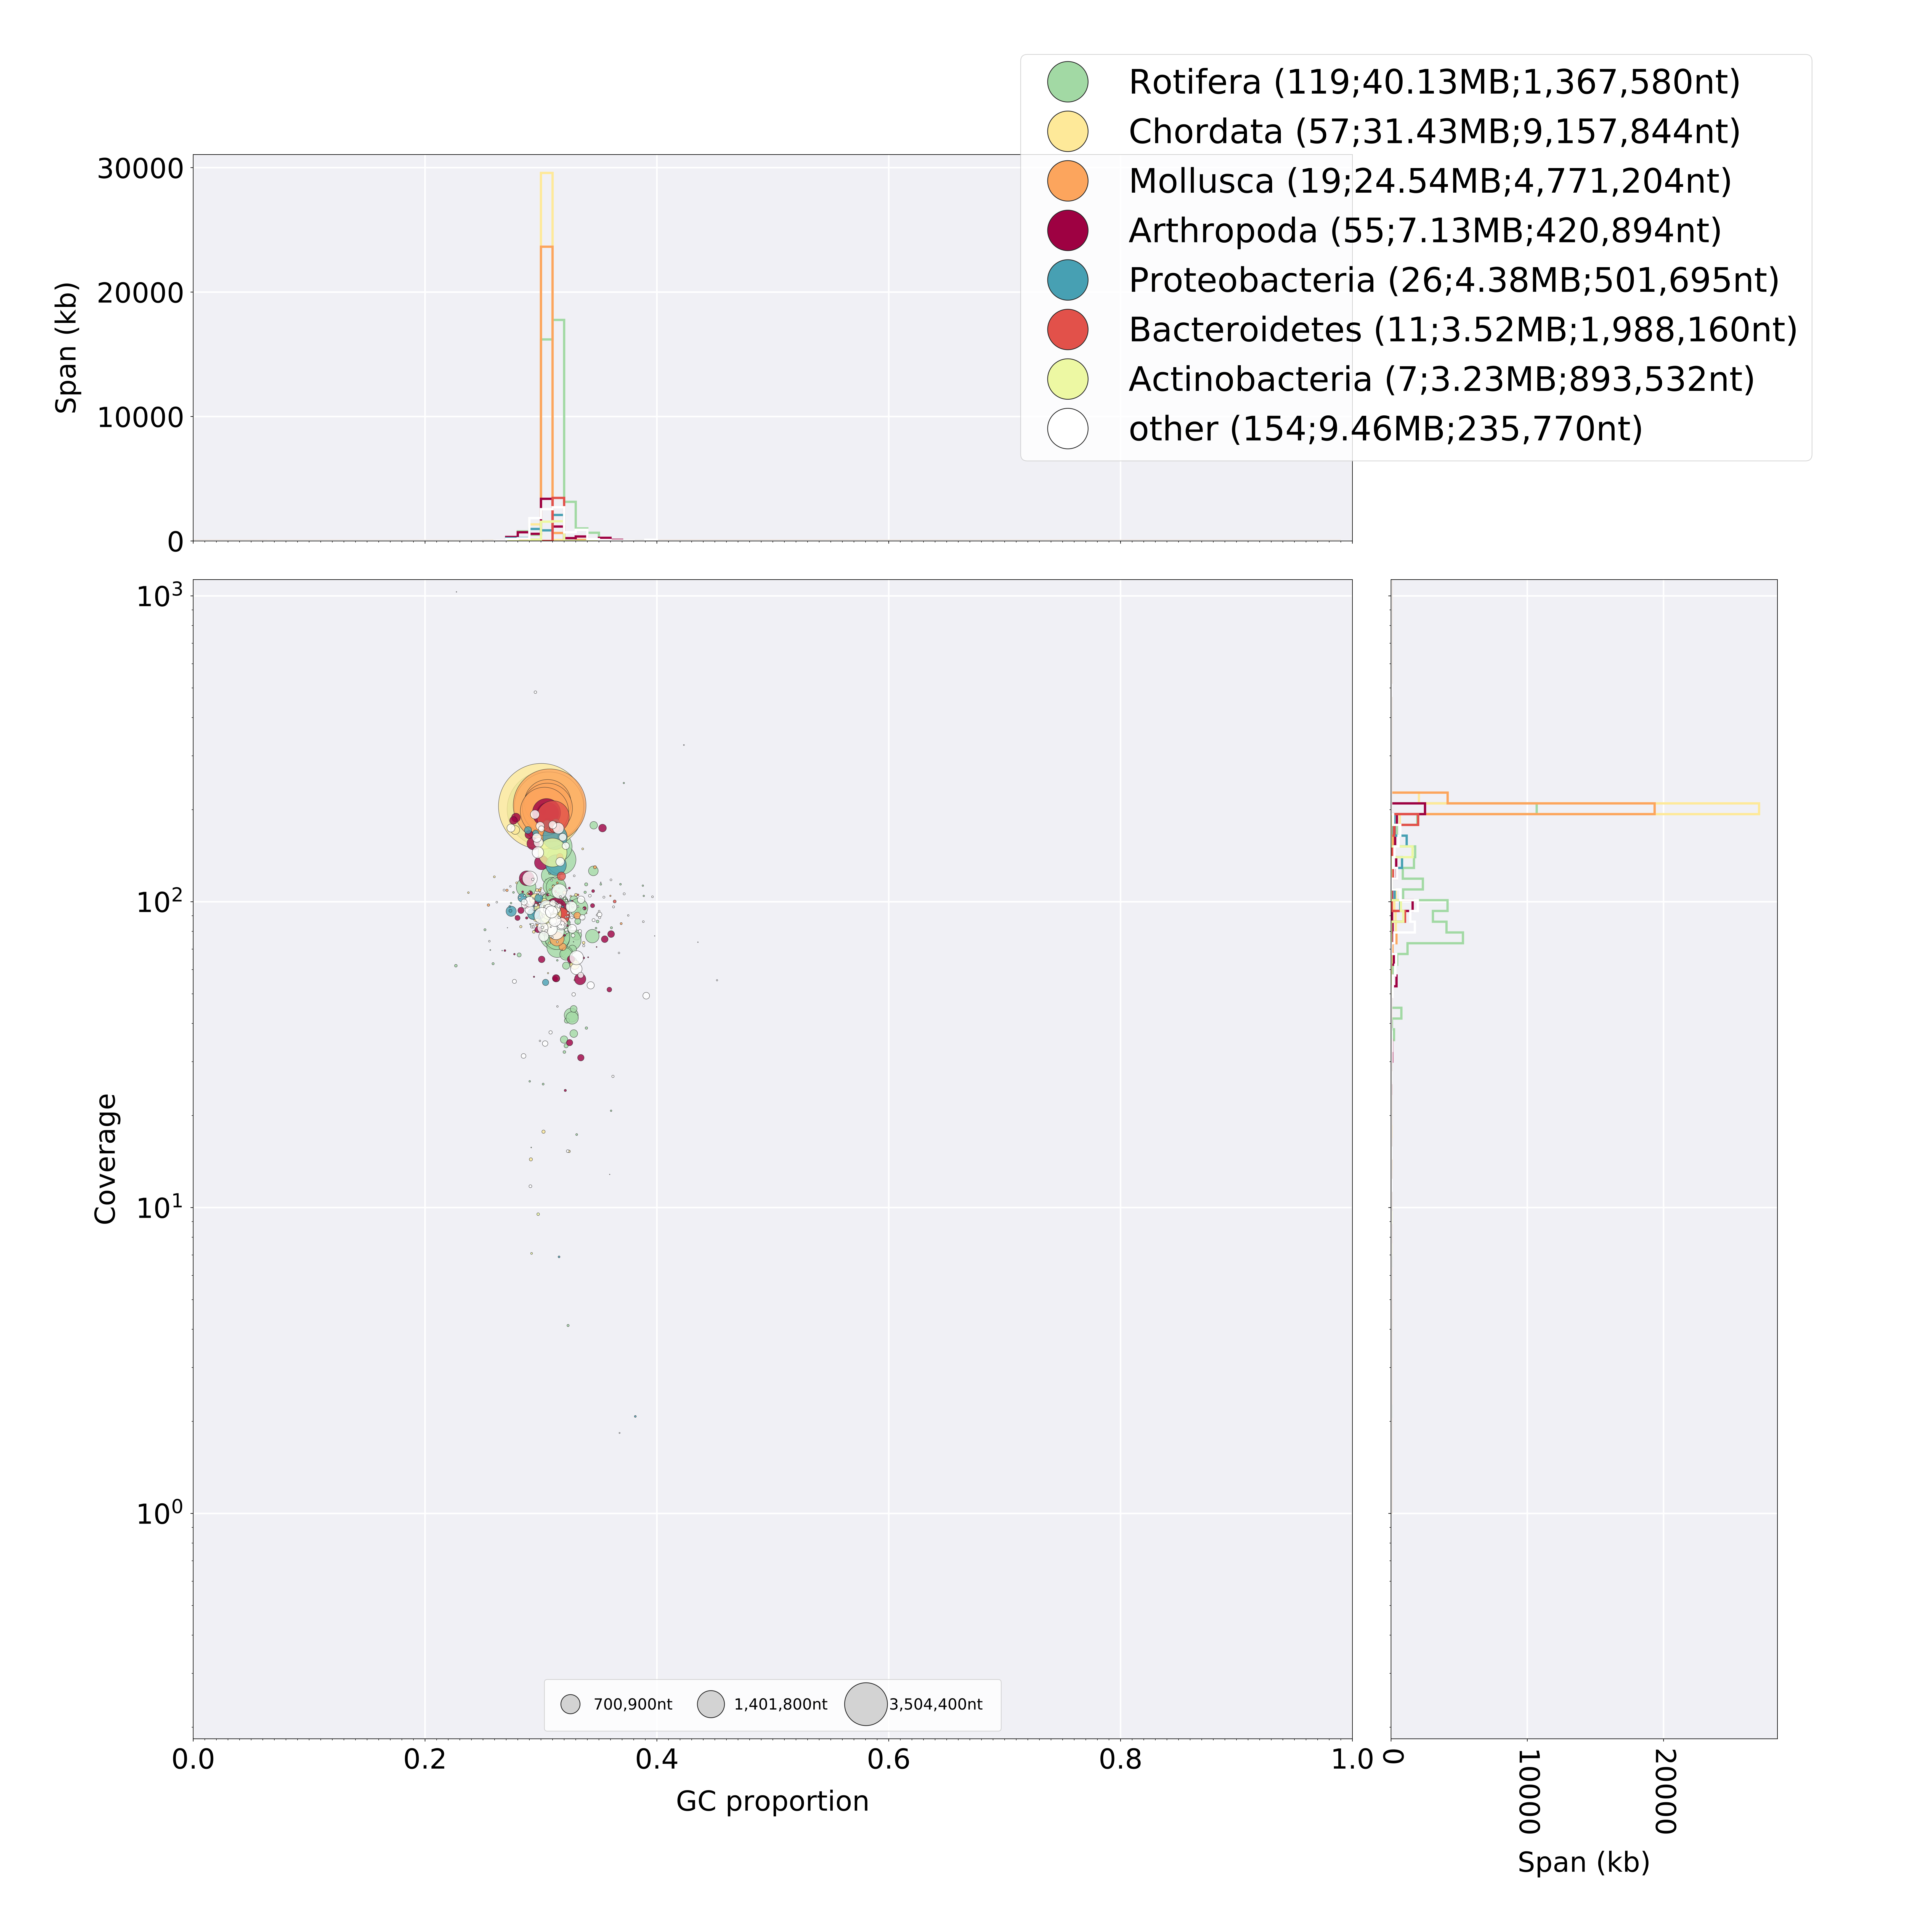
\includegraphics[width=15cm]{fig/benchmark/ONT_FLYE.png}
   \caption{Blobtools v1.0 analysis of a Flye assembly of the full Nanopore dataset.}
   \label{fig:blobtools_flye_ont}
 \end{figure}

  \begin{figure}[ht]
    \centering
     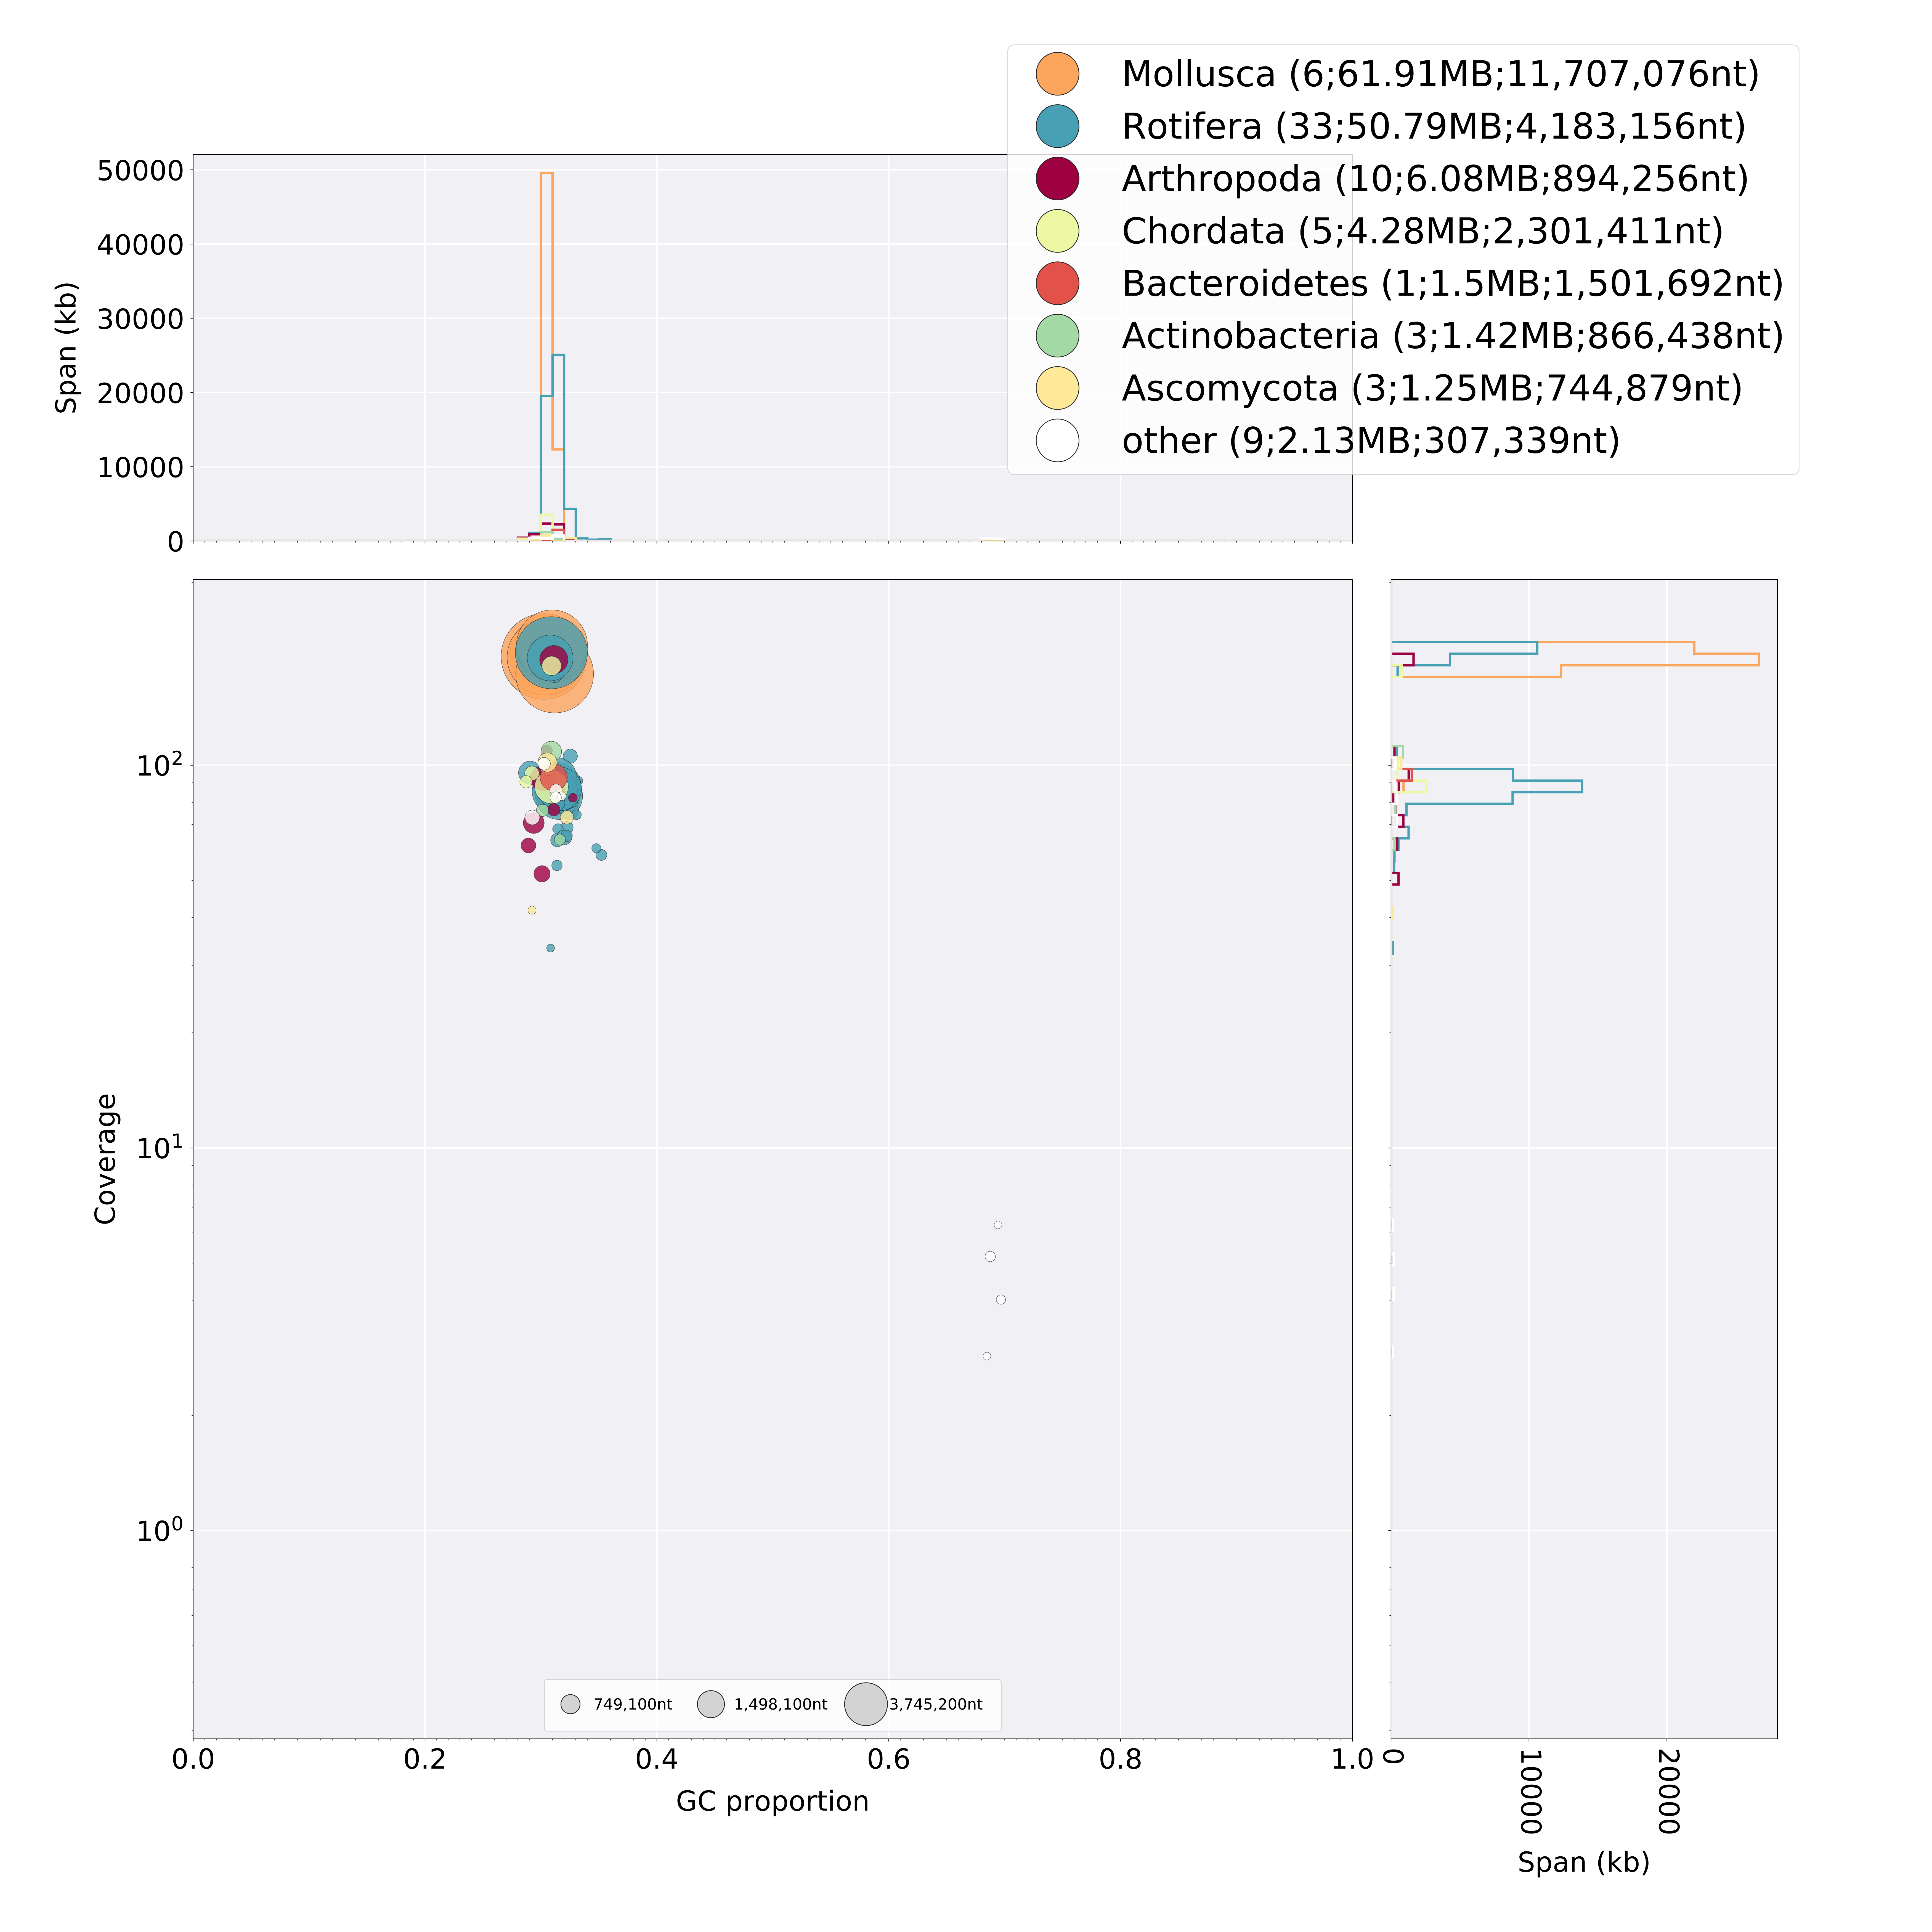
\includegraphics[width=15cm]{fig/benchmark/ONT_ND.png}
   \caption{Blobtools v1.0 analysis of a NextDenovo assembly of the full Nanopore dataset.}
   \label{fig:blobtools_NextDenovo_ont}
 \end{figure}

  \begin{figure}[ht]
    \centering
     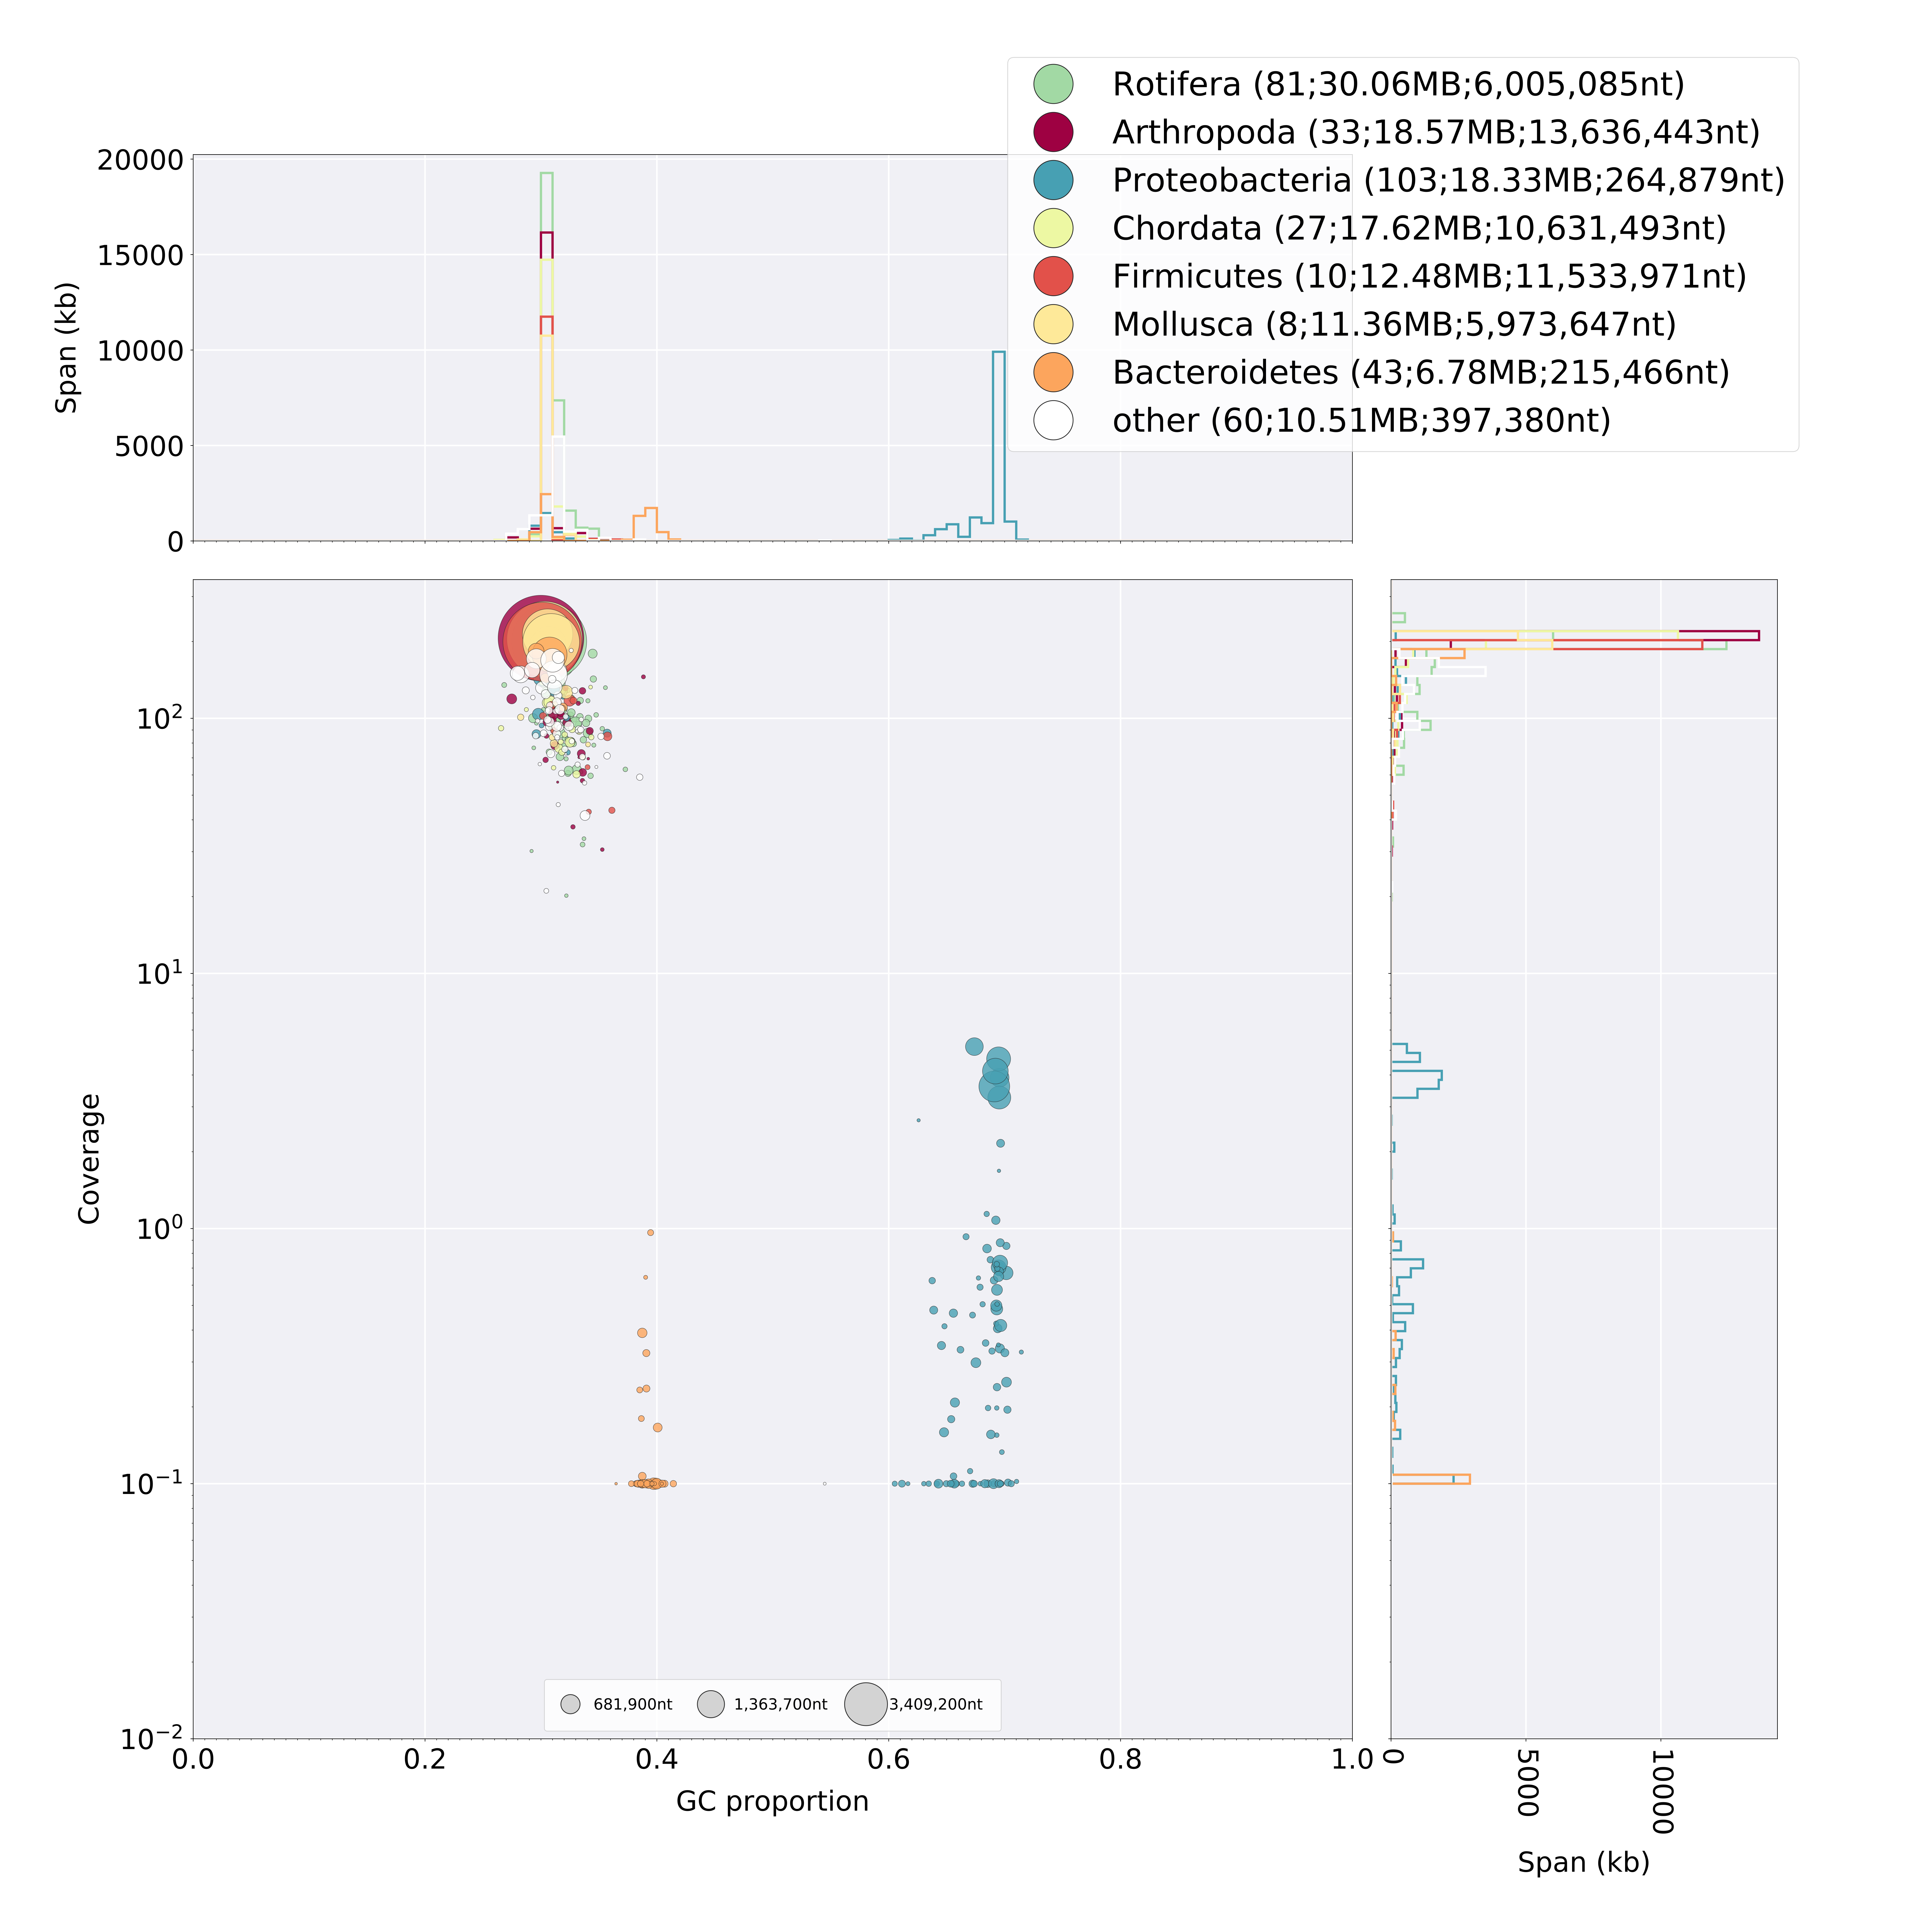
\includegraphics[width=15cm]{fig/benchmark/ONT_RA.png}
   \caption{Blobtools v1.0 analysis of a Ra assembly of the full Nanopore dataset.}
   \label{fig:blobtools_ra_ont}
 \end{figure}

  \begin{figure}[ht]
    \centering
     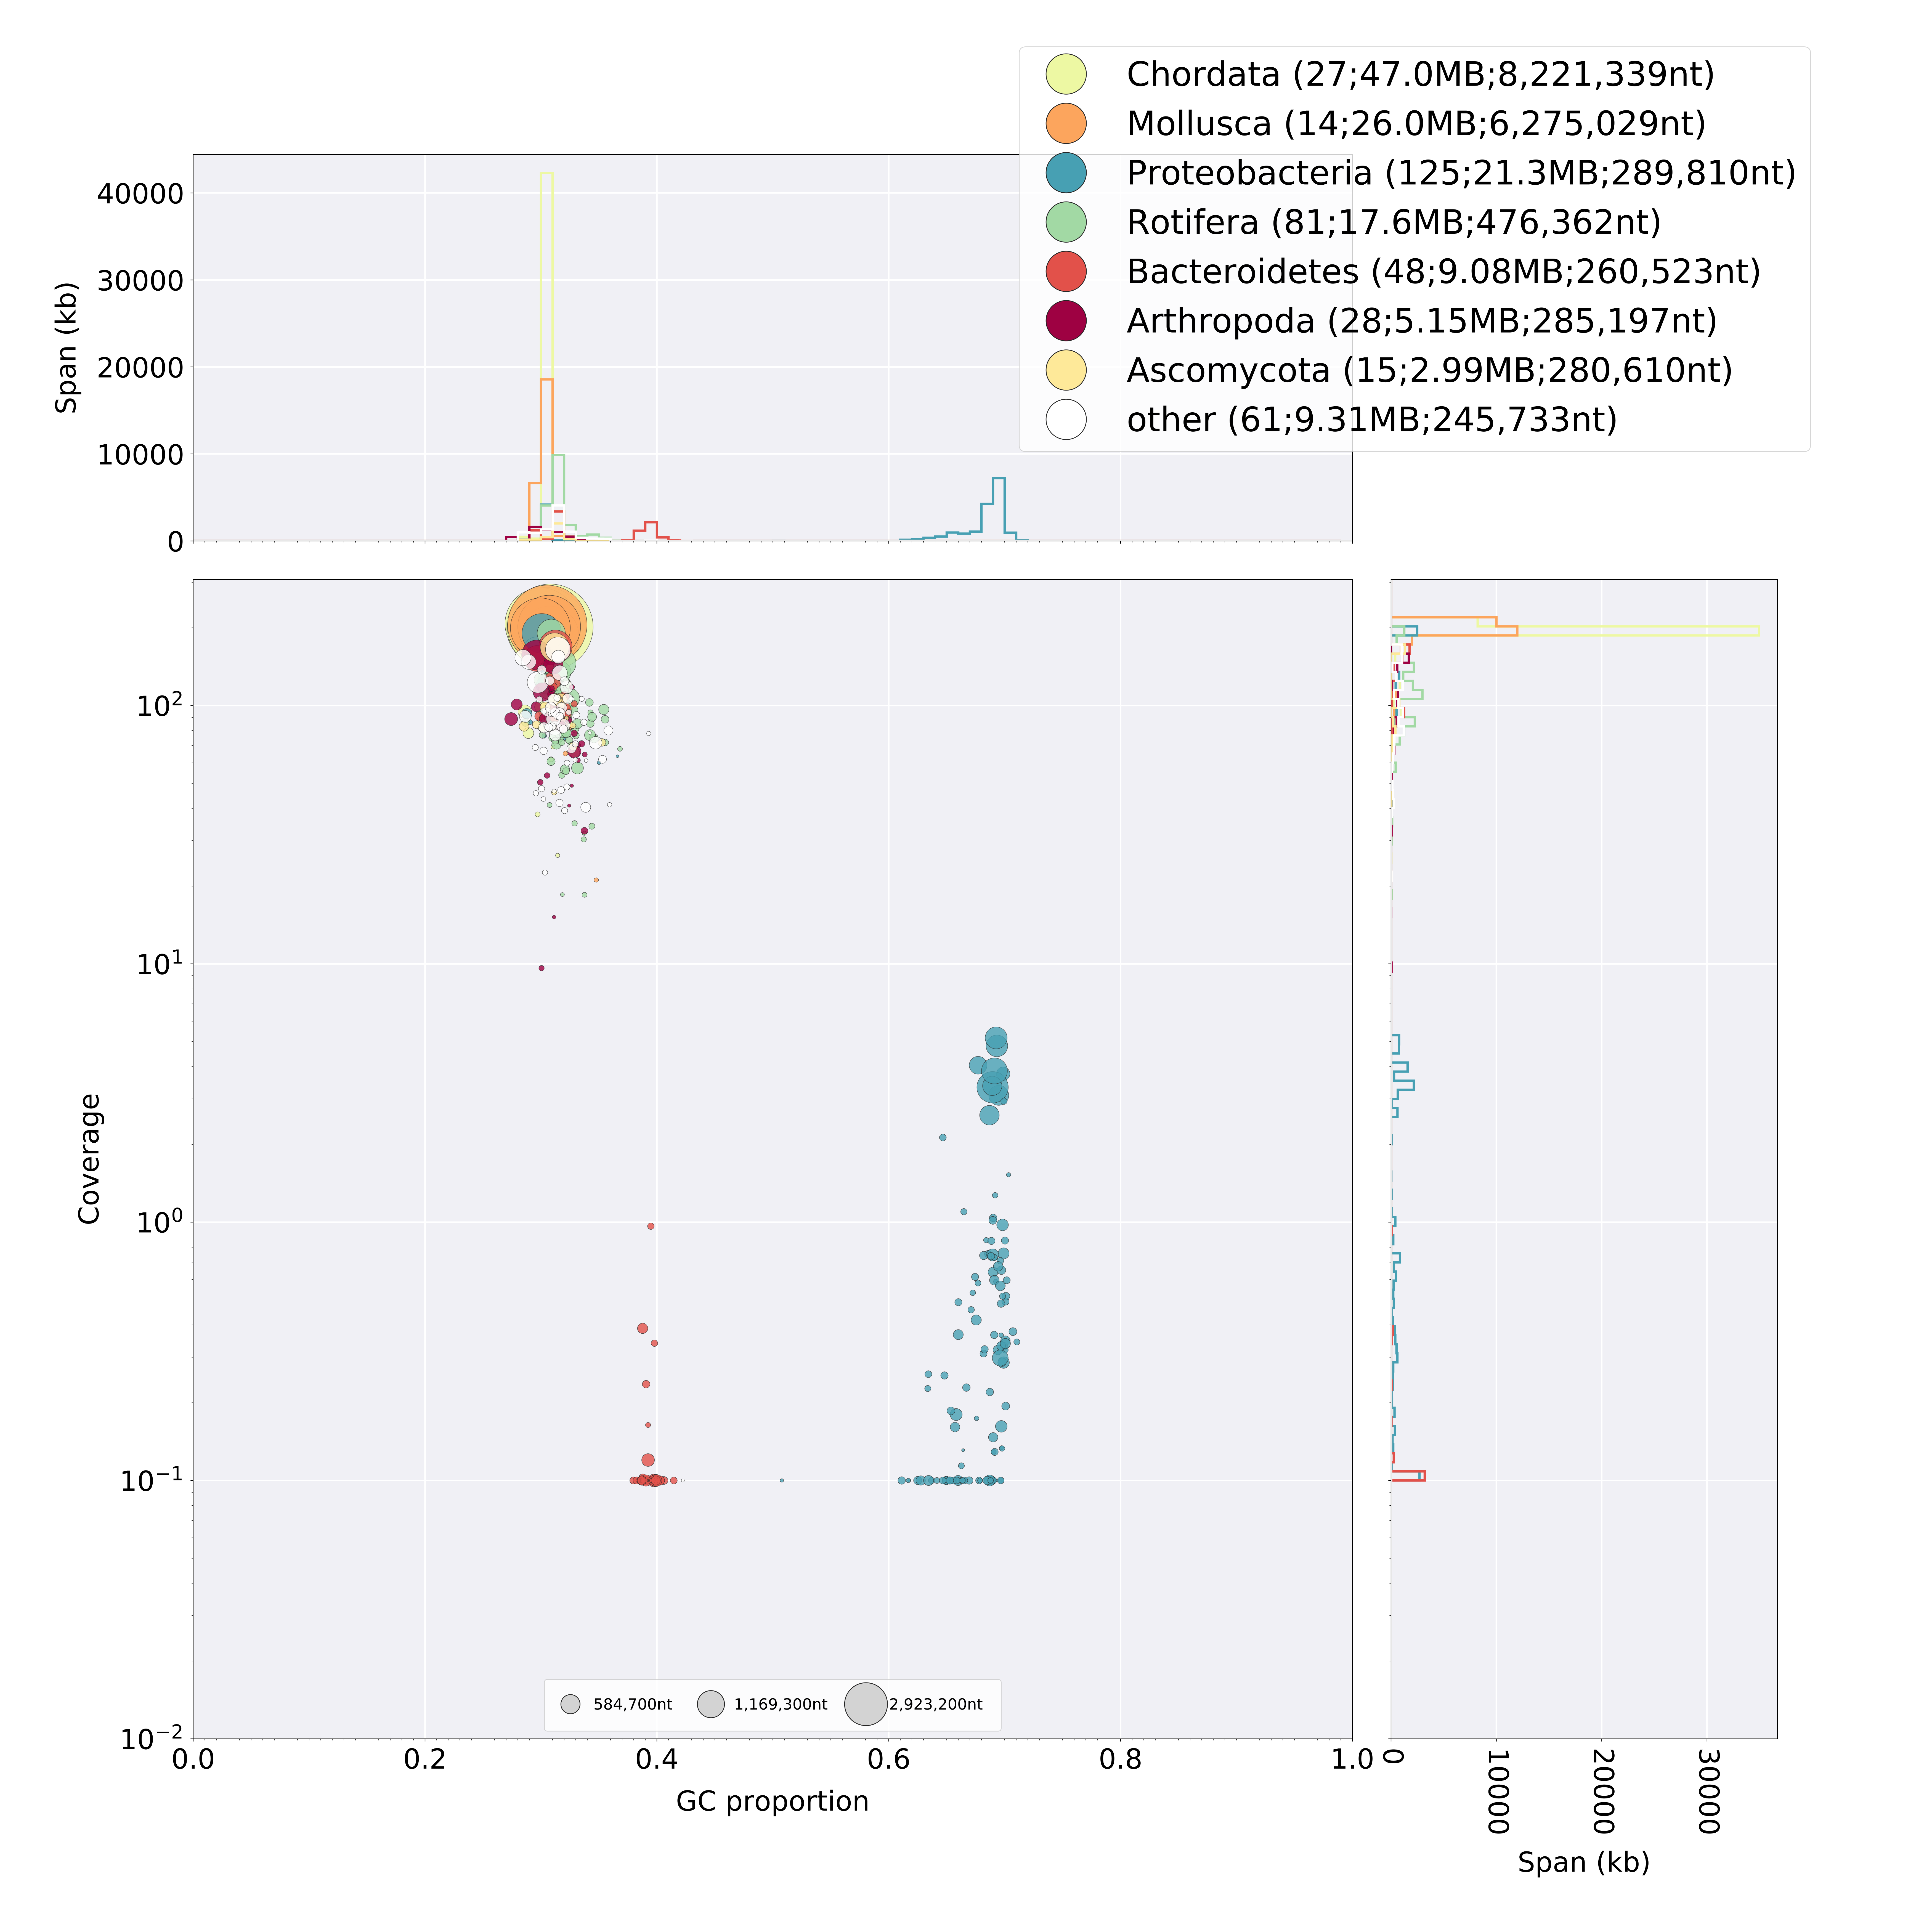
\includegraphics[width=15cm]{fig/benchmark/ONT_RAVEN.png}
   \caption{Blobtools v1.0 analysis of a Raven assembly of the full Nanopore dataset.}
   \label{fig:blobtools_raven_ont}
 \end{figure}

  \begin{figure}[ht]
    \centering
     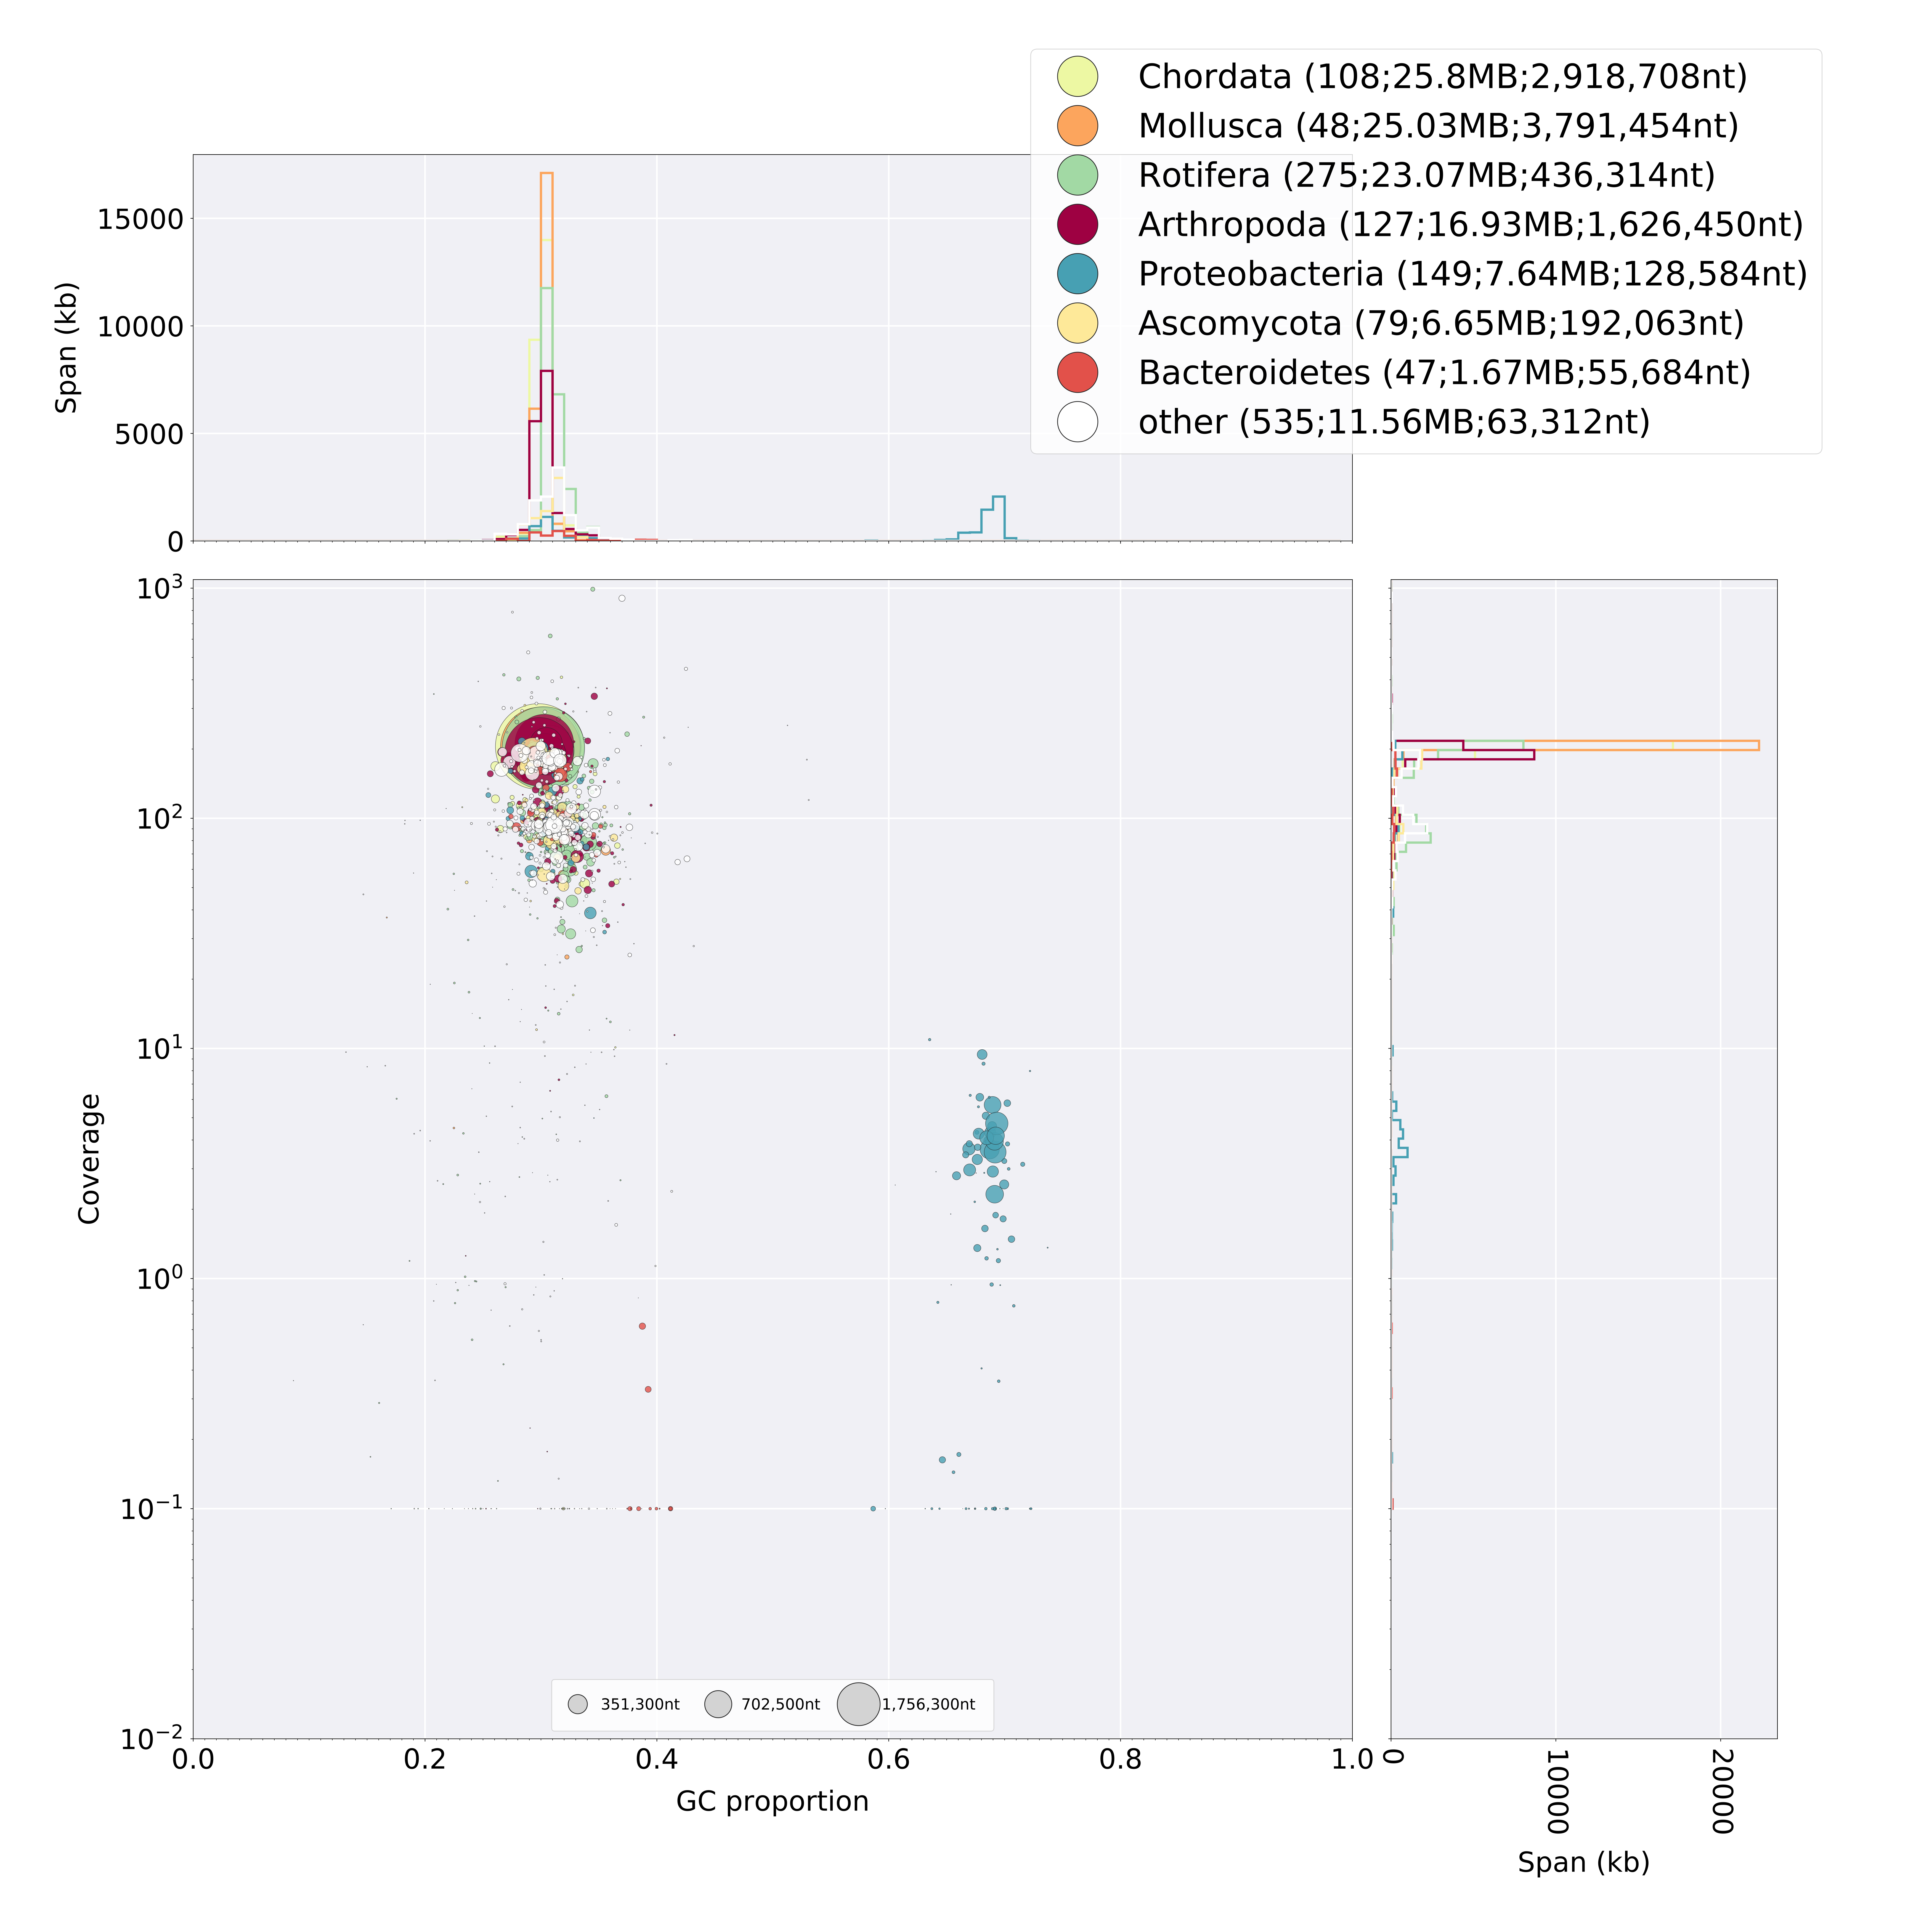
\includegraphics[width=15cm]{fig/benchmark/ONT_SHASTA.png}
   \caption{Blobtools v1.0 analysis of a Shasta assembly of the full Nanopore dataset.}
   \label{fig:blobtools_shasta_ont}
 \end{figure}

 \begin{figure}[ht]
    \centering
     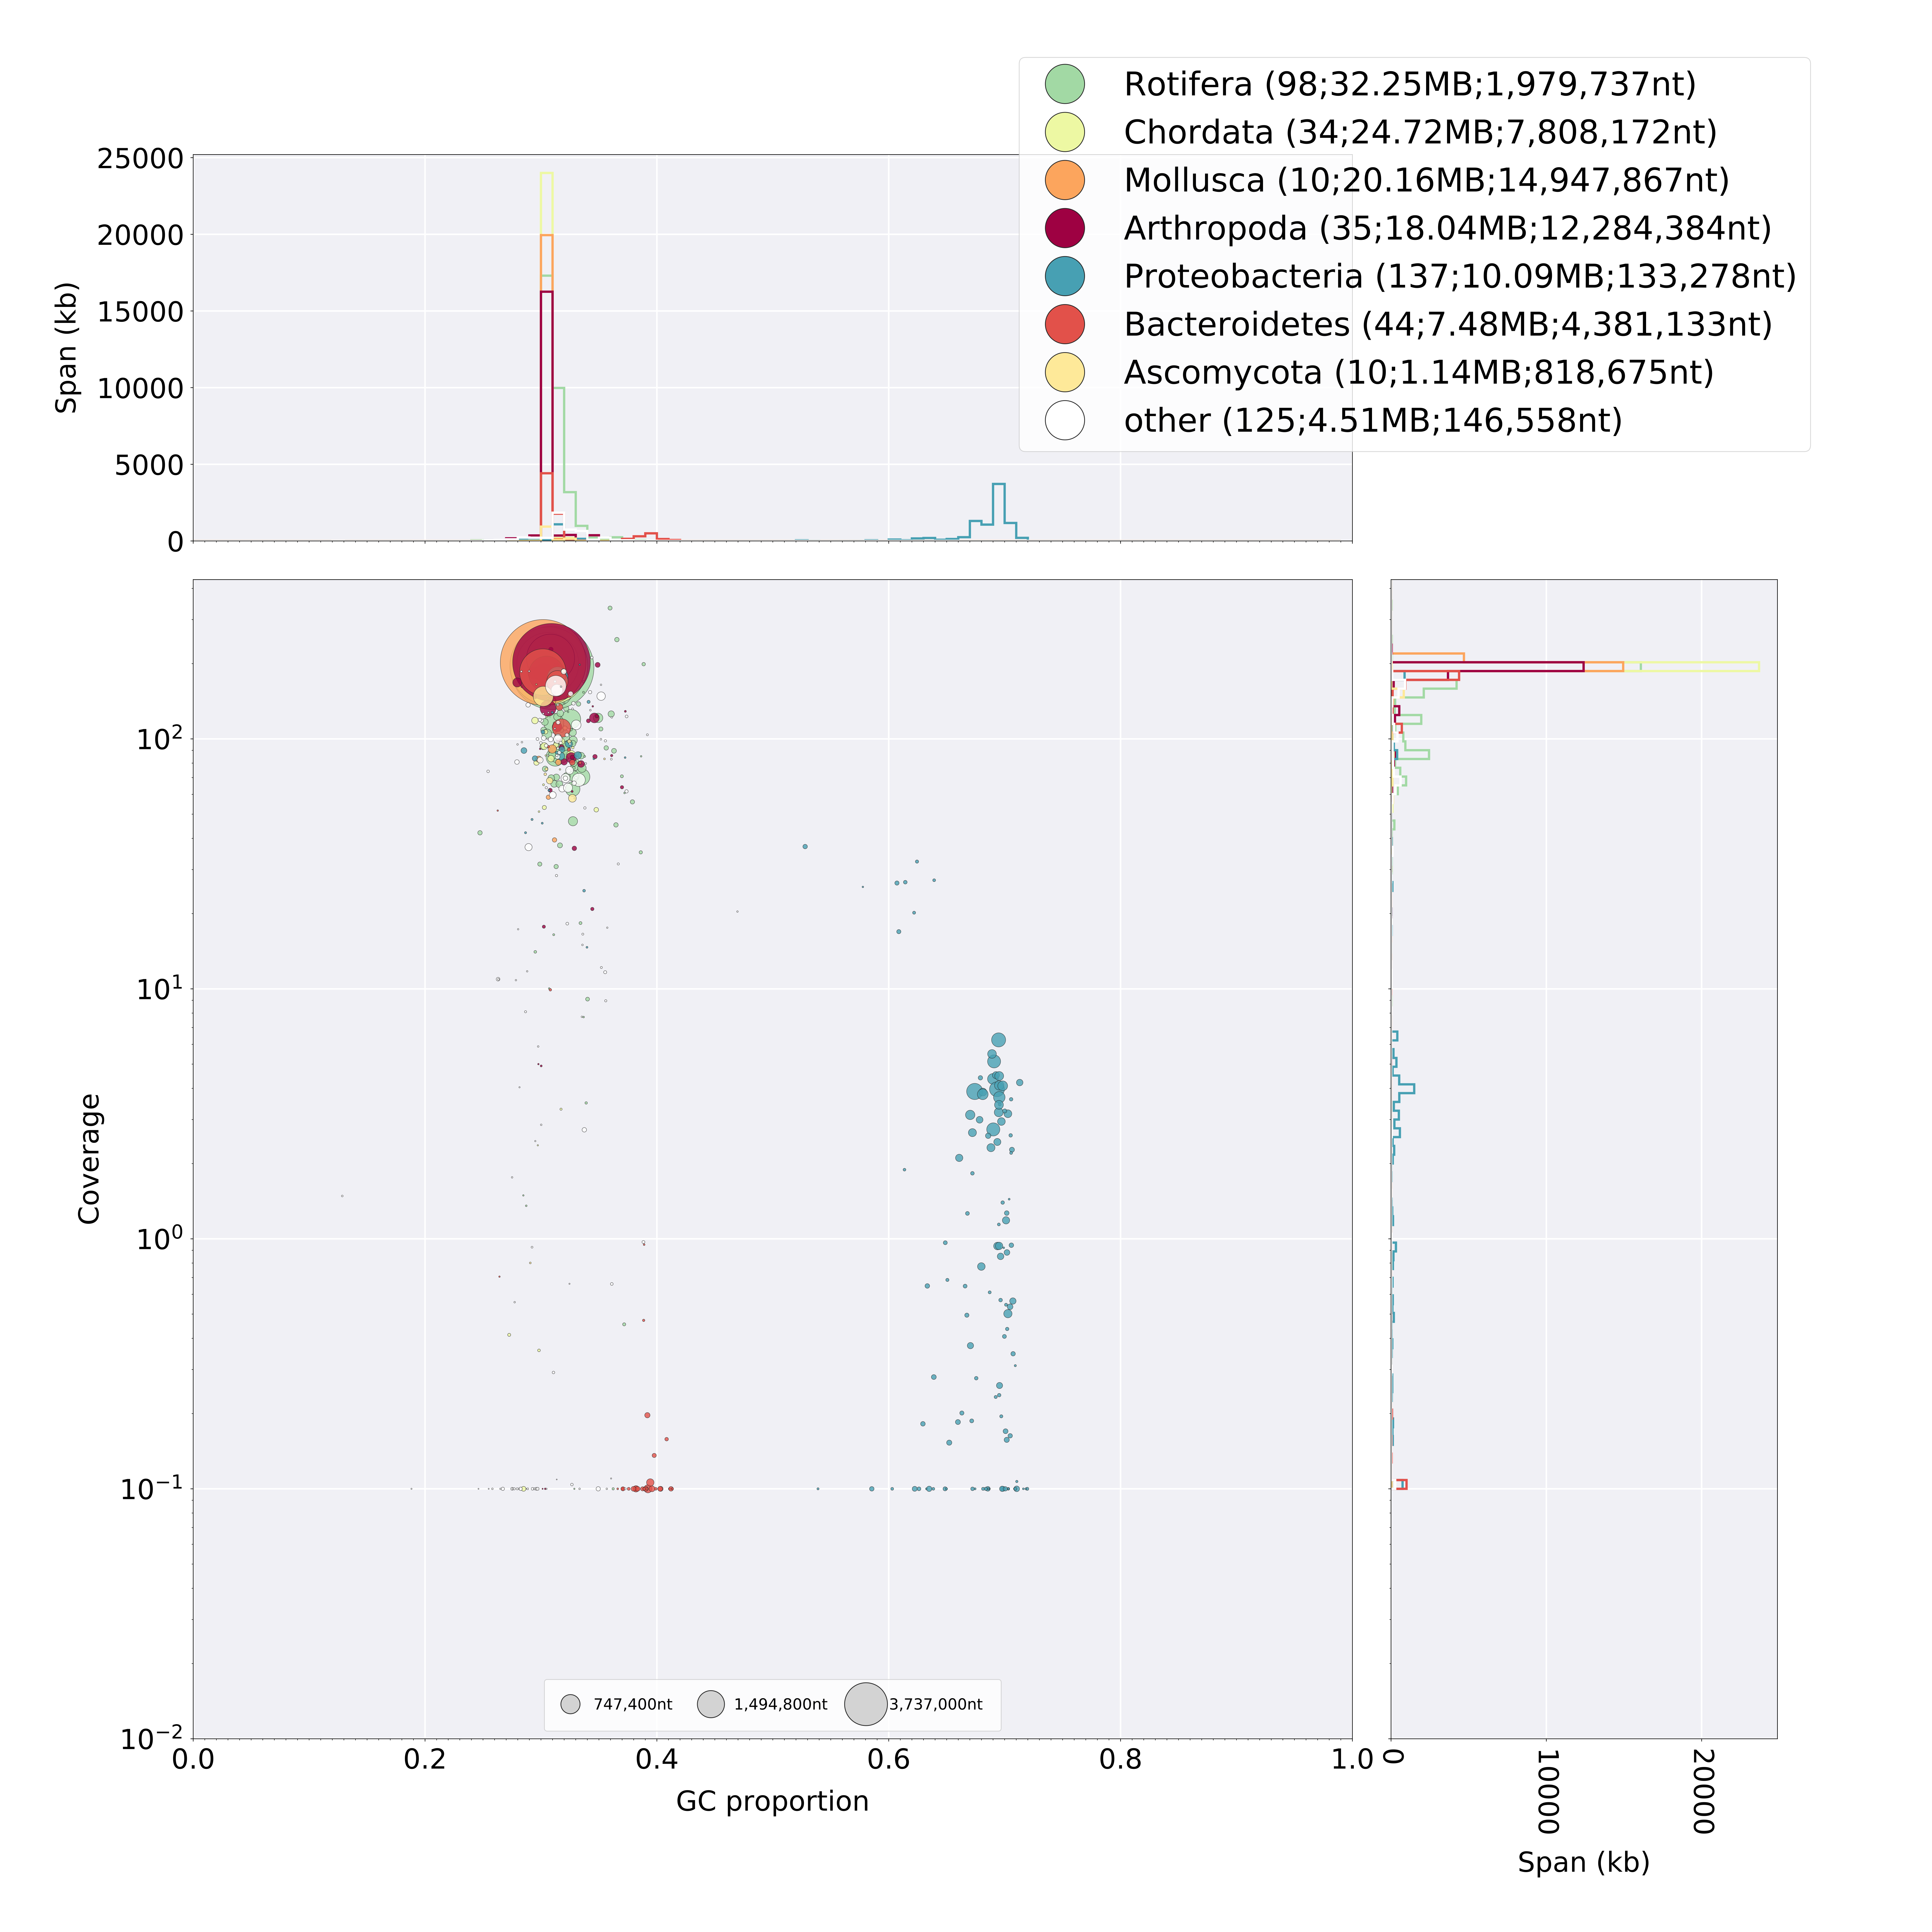
\includegraphics[width=15cm]{fig/benchmark/ONT_WTDBG.png}
   \caption{Blobtools v1.0 analysis of a wtdbg2 assembly of the full Nanopore dataset.}
   \label{fig:blobtools_wtdbg_ont}
 \end{figure}


     \begin{figure}[ht]
    \centering
     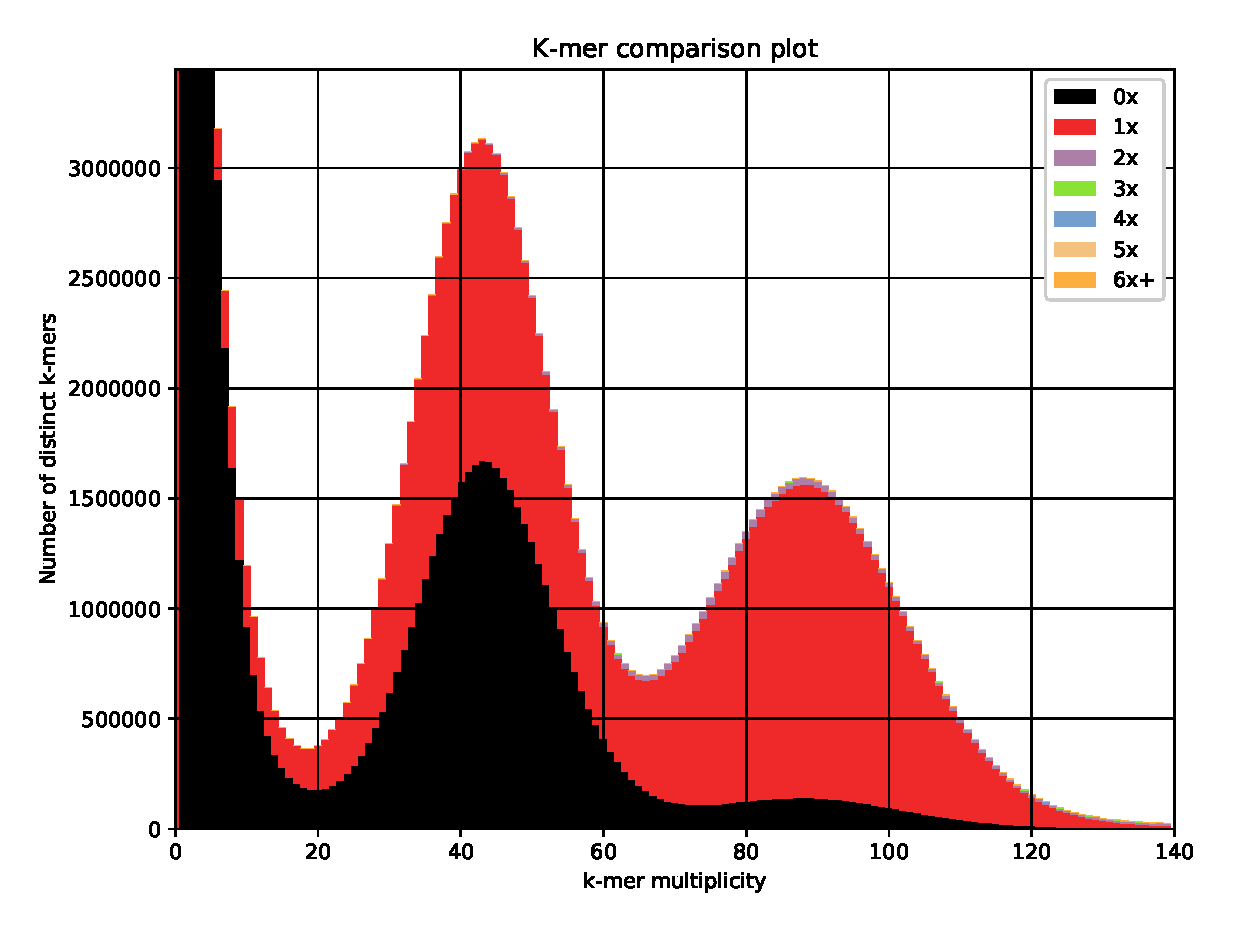
\includegraphics[width=13.5cm]{fig/benchmark/kat_comp_shasta_1-main.mx.spectra-cn.eps}
   \caption{\textit{k}-mer spectrum of the Shasta assembly of the full Nanopore dataset obtained with KAT v2.4.2.}
   \label{fig:kat_shasta_all}
 \end{figure}
 
    \begin{figure}[ht]
    \centering
     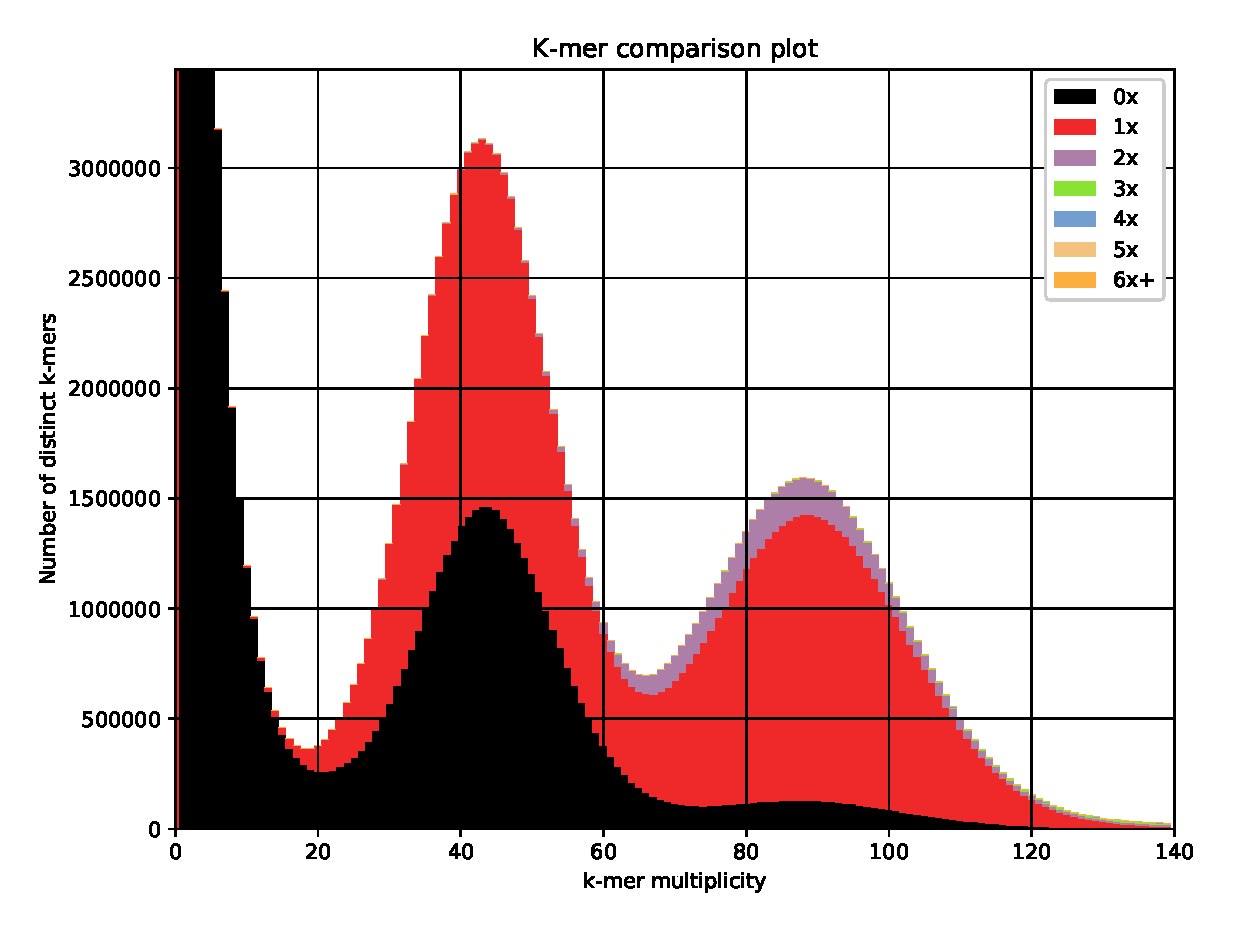
\includegraphics[width=13.5cm]{fig/benchmark/kat_comp_shasta_min30000_1-main.mx.spectra-cn.eps}
   \caption{\textit{k}-mer spectrum of the Shasta assembly of the longest Nanopore reads obtained with KAT v2.4.2.}
   \label{fig:kat_shasta_min30000}
 \end{figure}
 
    \begin{figure}[ht]
    \centering
     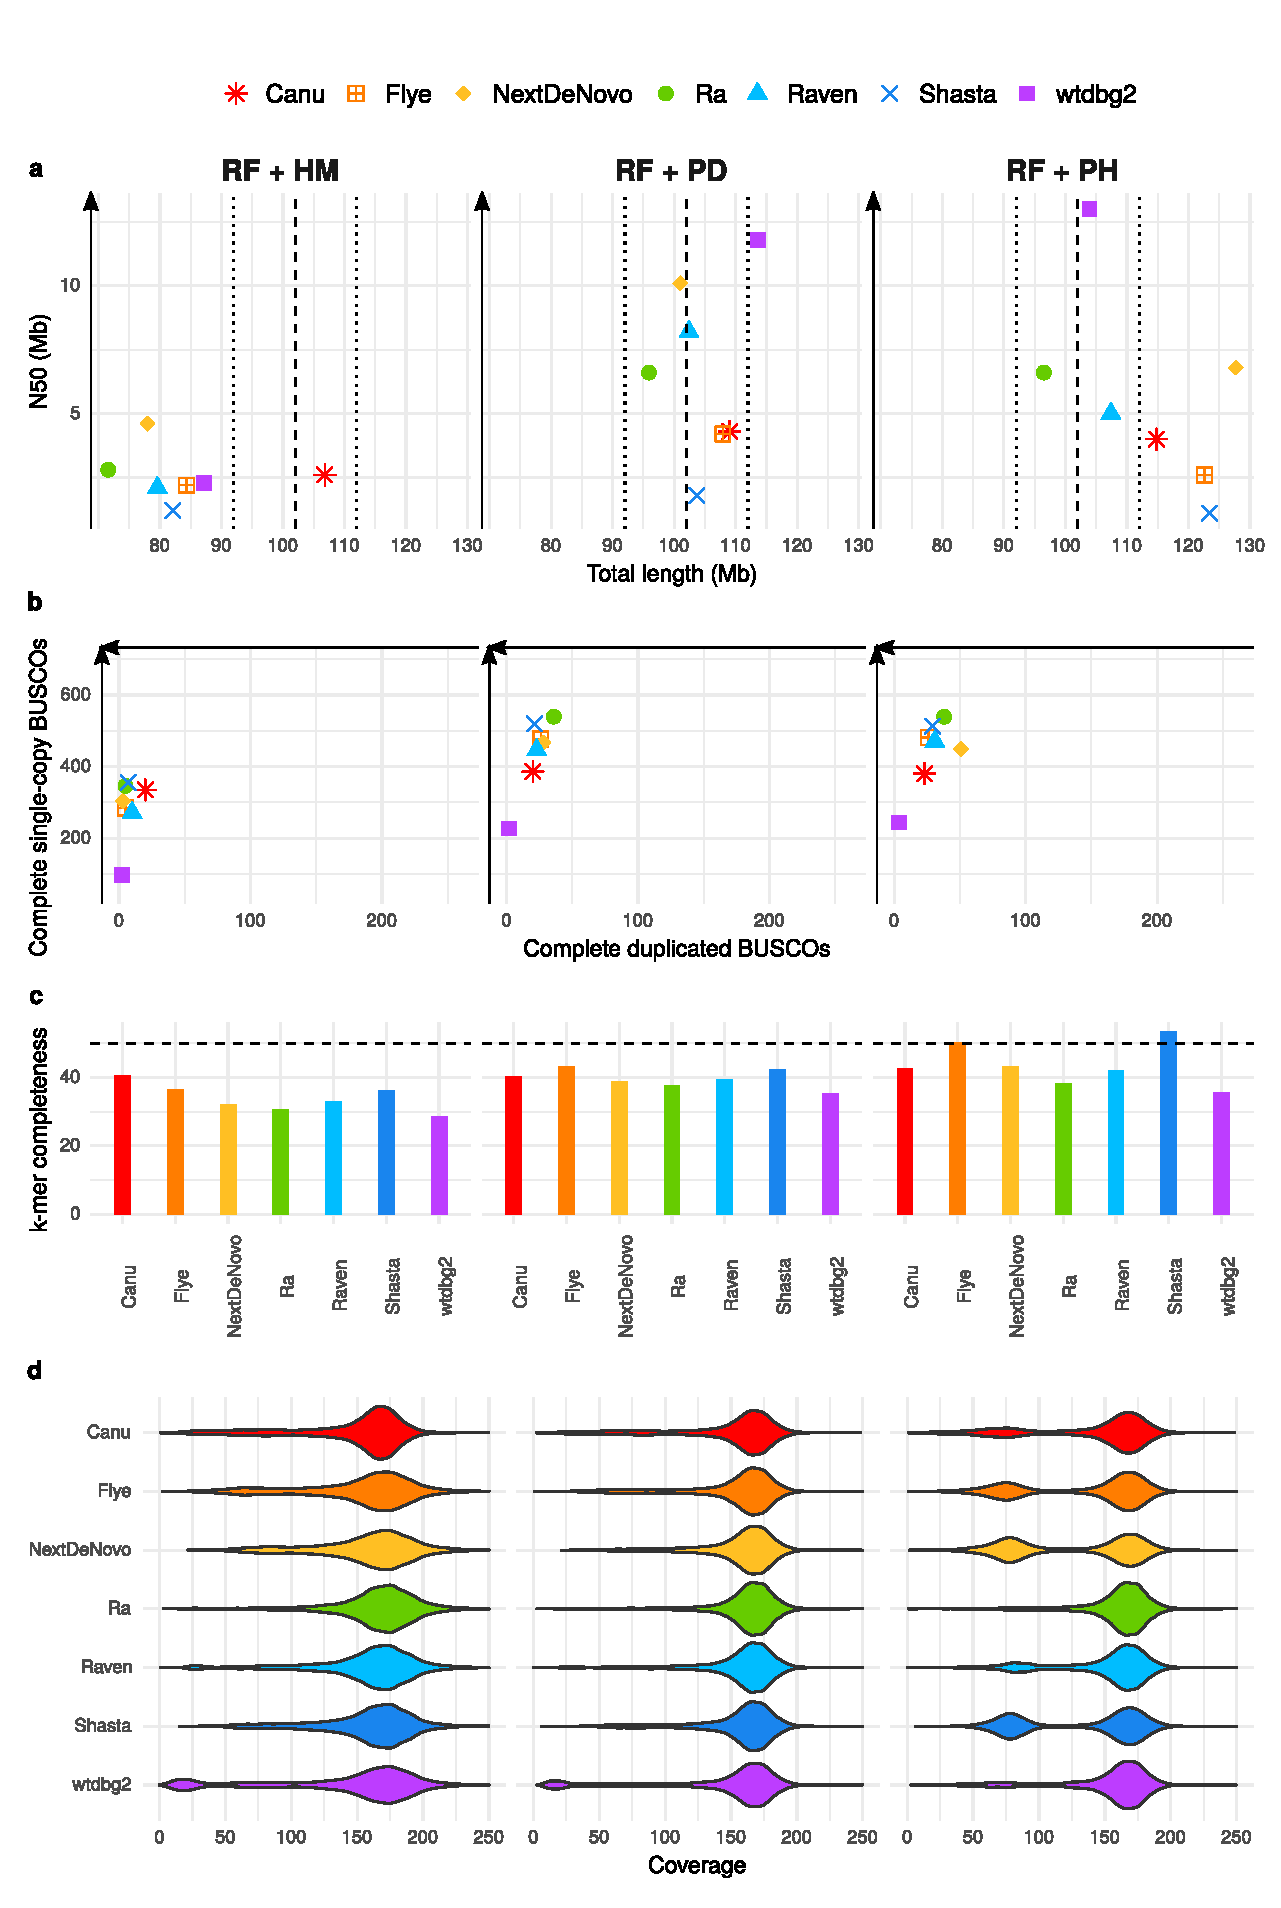
\includegraphics[width=13.5cm]{fig/benchmark/supp_nanopore_filtering_purging_v20201012.eps}
   \caption{Statistics of Nanopore assemblies obtained from the filtered Nanopore dataset of reads longer than 30 kb, with a subsequent removal of uncollapsed haplotypes with HaploMerger2 (HM), purge\_dups (PD), or purge\_haplotigs (PH). a) N50 plotted against total assembly length. The dashed line indicates the expected genome size, with a +/- 10 Mb margin delimited by the dotted lines. b) Number of complete single-copy BUSCOs plotted against number of complete duplicated BUSCOs, from a total of 954 orthologs. c) \textit{k}-mer completeness. The dashed line indicates the expected 50\% completeness. d) Long-read coverage distribution over the contigs.}
   \label{fig:nanopore_filtering_purging}
 \end{figure}
 
     \begin{figure}[ht]
    \centering
     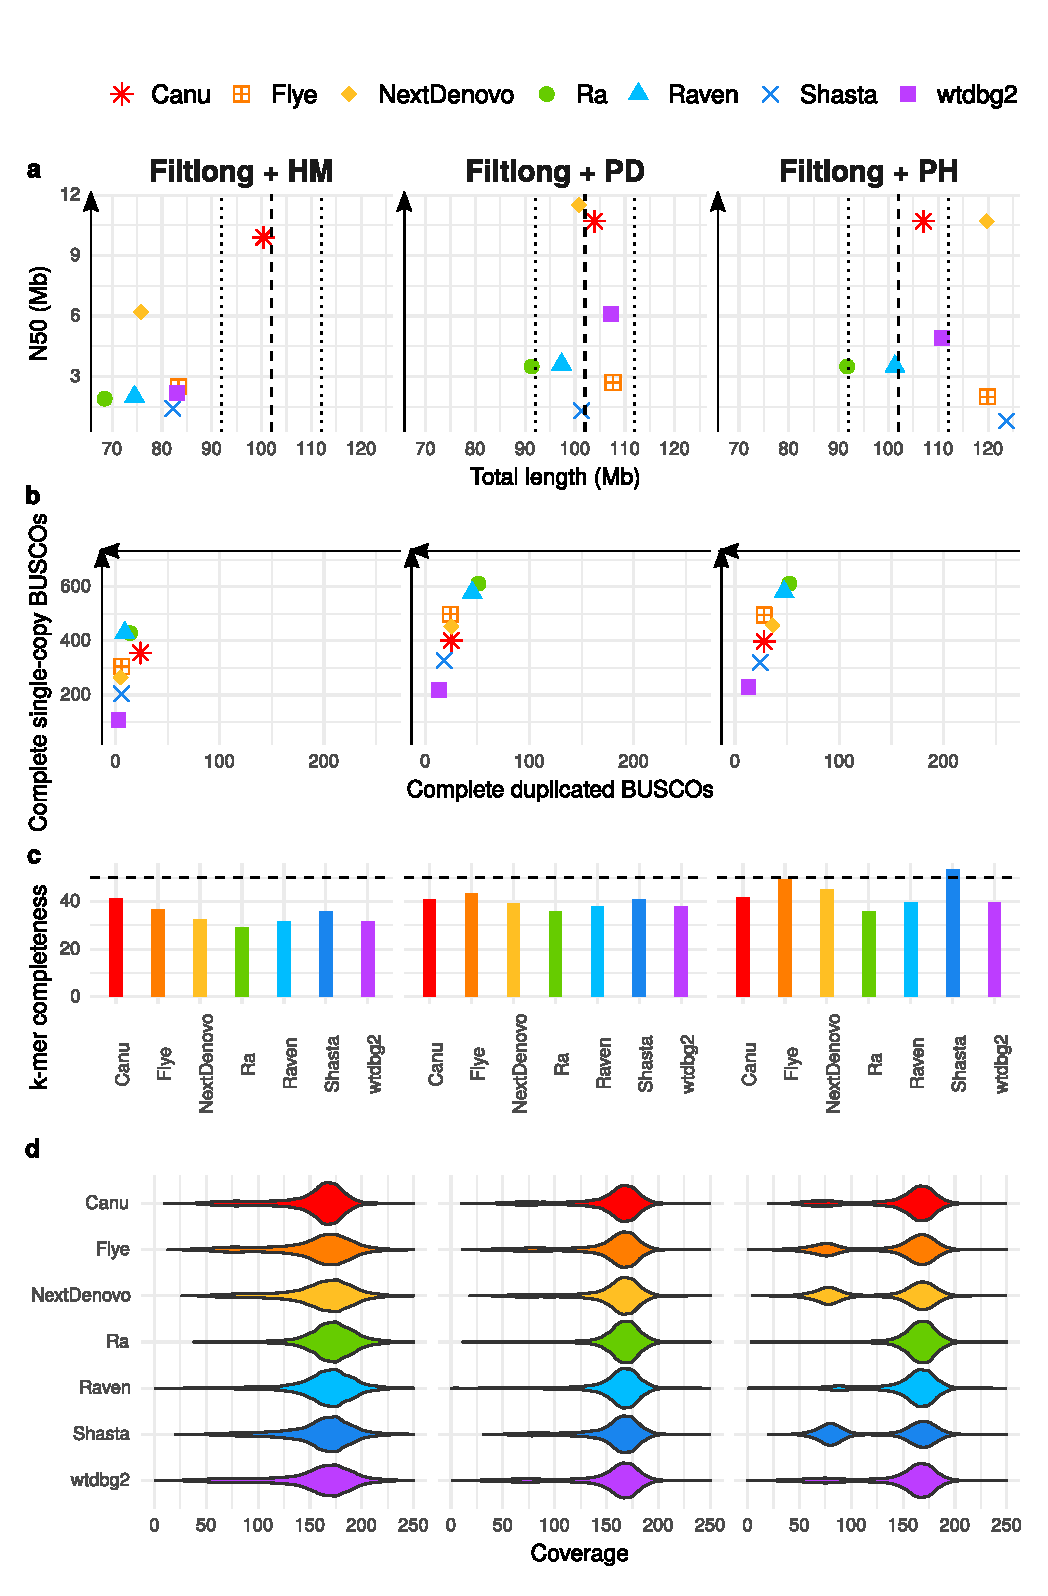
\includegraphics[width=13.5cm]{fig/benchmark/supp_nanopore_filtlong_purging_v20210310.eps}
   \caption{Statistics of Nanopore assemblies obtained from the Nanopore dataset filtered with Filtlong, with a subsequent removal of uncollapsed haplotypes with HaploMerger2 (HM), purge\_dups (PD), or purge\_haplotigs (PH). a) N50 plotted against total assembly length. The dashed line indicates the expected genome size, with a +/- 10 Mb margin delimited by the dotted lines. b) Number of complete single-copy BUSCOs plotted against number of complete duplicated BUSCOs, from a total of 954 orthologs. c) \textit{k}-mer completeness. The dashed line indicates the expected 50\% completeness. d) Long-read coverage distribution over the contigs.}
   \label{fig:nanopore_filtlong_purging}
 \end{figure}
 
   \begin{figure}[ht]
    \centering
     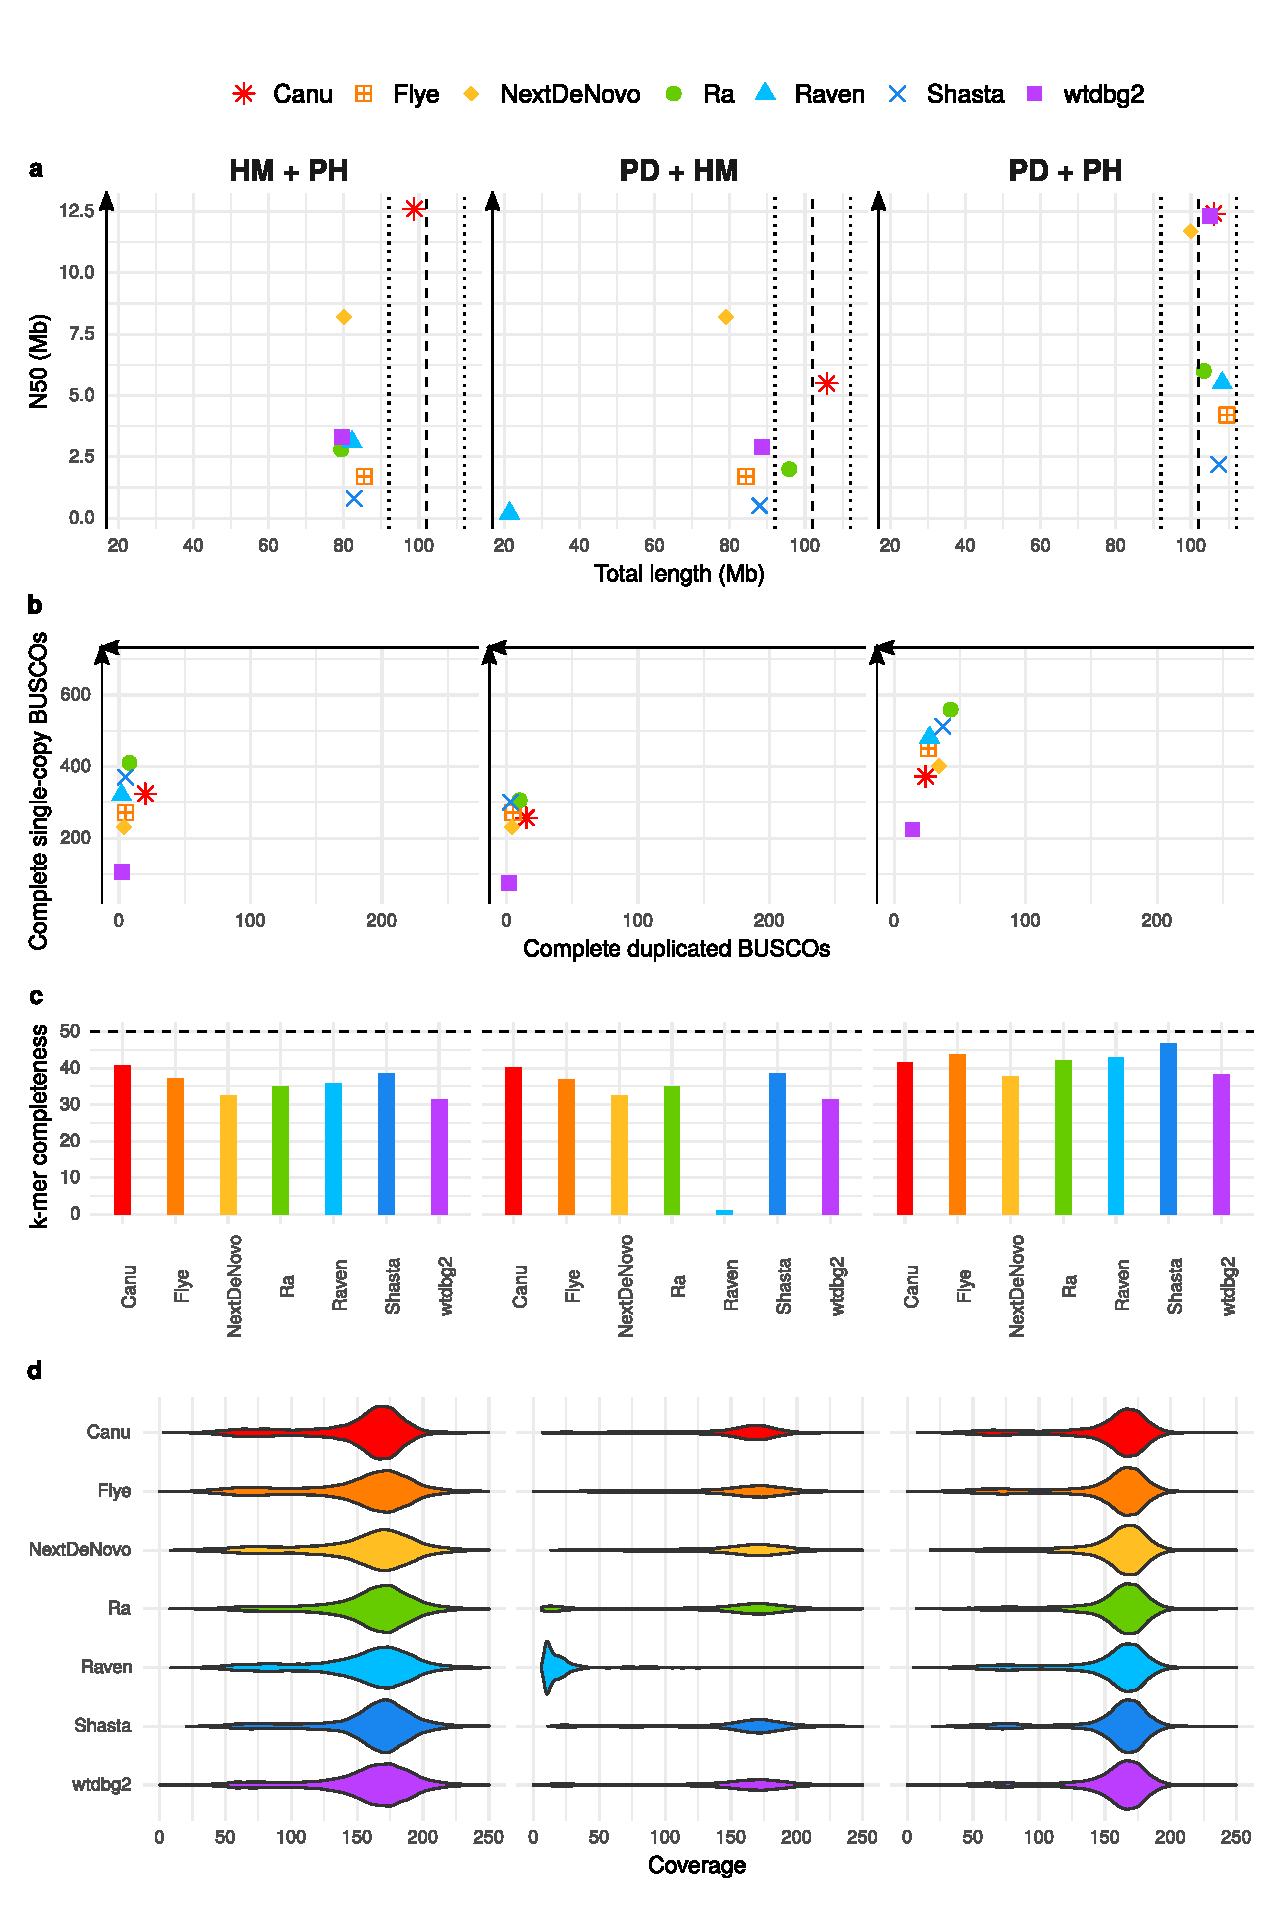
\includegraphics[width=13.5cm]{fig/benchmark/supp_nanopore_purging_combinations_v20200919.eps}
   \caption{Statistics of Nanopore assemblies obtained from the full Nanopore dataset with a subsequent removal of uncollapsed haplotypes with combinations of HaploMerger2 (HM), purge\_dups (PD), and purge\_haplotigs (PH). a) N50 plotted against total assembly length. The dashed line indicates the expected genome size, with a +/- 10 Mb margin delimited by the dotted lines. b) Number of complete single-copy BUSCOs plotted against number of complete duplicated BUSCOs, from a total of 954 orthologs. c) \textit{k}-mer completeness. The dashed line indicates the expected 50\% completeness. d) Long-read coverage distribution over the contigs.}
   \label{fig:nanopore_purging_combinations}
 \end{figure}
 
\begin{table}[ht]
\centering
\caption{Haploidy values computed by HapPy v0.1 for PacBio assemblies.}
\begin{adjustbox}{totalheight=\textheight-2\baselineskip}
\begin{tabular}{llc}
\hline
\textbf{Assembler} & \textbf{Processing} & \textbf{Haploidy} \\
\hline
Canu & raw assemblies & 0.59 \\
Flye & raw assemblies & 0.85 \\
NextDenovo & raw assemblies & 0.81 \\
Ra & raw assemblies & 0.90 \\
Raven & raw assemblies & 0.82 \\
Shasta & raw assemblies & 0.83 \\
wtdbg2 & raw assemblies & 0.90 \\
Canu & longest reads & 0.62 \\
Flye & longest reads & 0.85 \\
NextDenovo & longest reads & 0.94 \\
Ra & longest reads & 0.94 \\
Raven & longest reads & 0.88 \\
Shasta & longest reads & 0.96 \\
wtdbg2 & longest reads & 0.90 \\
Canu & Filtlong & 0.58 \\
Flye & Filtlong & 0.86 \\
NextDenovo & Filtlong & 0.88 \\
Ra & Filtlong & 0.94 \\
Raven & Filtlong & 0.90 \\
Shasta & Filtlong & 0.85 \\
wtdbg2 & Filtlong & 0.91 \\
Canu & HaploMerger2 & 0.84 \\
Flye & HaploMerger2 & 0.89 \\
NextDenovo & HaploMerger2 & 0.88 \\
Ra & HaploMerger2 & 0.92 \\
Raven & HaploMerger2 & 0.90 \\
Shasta & HaploMerger2 & 0.91 \\
wtdbg2 & HaploMerger2 & 0.92 \\
Canu & purge\_dups & 0.89 \\
Flye & purge\_dups & 0.89 \\
NextDenovo & purge\_dups & 0.90 \\
Ra & purge\_dups & 0.91 \\
Raven & purge\_dups & 0.90 \\
Shasta & purge\_dups & 0.90 \\
wtdbg2 & purge\_dups & 0.91 \\
Canu & purge\_haplotigs & 0.86 \\
Flye & purge\_haplotigs & 0.85 \\
NextDenovo & purge\_haplotigs & 0.87 \\
Ra & purge\_haplotigs & 0.88 \\
Raven & purge\_haplotigs & 0.80 \\
Shasta & purge\_haplotigs & 0.90 \\
wtdbg2 & purge\_haplotigs & 0.90 \\
\hline
\end{tabular}
\end{adjustbox}
\label{tab:pacbio_happy_part1}
\end{table}

\begin{table}[ht]
\centering
\caption{Haploidy values computed by HapPy v0.1 for PacBio assemblies.}
\begin{tabular}{llc}
\hline
\textbf{Assembler} & \textbf{Processing} & \textbf{Haploidy} \\
\hline
Canu & longest reads $+$ purge\_haplotigs & 0.87 \\ \
Flye & longest reads $+$ purge\_haplotigs & 0.85 \\
NextDenovo & longest reads $+$ purge\_haplotigs & 0.94 \\
Ra & longest reads $+$ purge\_haplotigs & 0.92 \\
Raven & longest reads $+$ purge\_haplotigs & 0.87 \\
Shasta & longest reads $+$ purge\_haplotigs & 0.96 \\
wtdbg2 & longest reads $+$ purge\_haplotigs & 0.90 \\
Canu & longest reads $+$ purge\_dups & 0.91 \\
Flye & longest reads $+$ purge\_dups & 0.90 \\
NextDenovo & longest reads $+$ purge\_dups & 0.97 \\
Ra & longest reads $+$ purge\_dups & 0.95 \\
Raven & longest reads $+$ purge\_dups & 0.91 \\
Shasta & longest reads $+$ purge\_dups & 0.97 \\
wtdbg2 & longest reads $+$ purge\_dups & 0.92 \\
Canu & Filtlong $+$ purge\_haplotigs & 0.56 \\ \
Flye & Filtlong $+$ purge\_haplotigs & 0.86 \\
NextDenovo & Filtlong $+$ purge\_haplotigs & 0.88 \\
Ra & Filtlong $+$ purge\_haplotigs & 0.93 \\
Raven & Filtlong $+$ purge\_haplotigs & 0.90 \\
Shasta & Filtlong $+$ purge\_haplotigs & 0.85 \\
wtdbg2 & Filtlong $+$ purge\_haplotigs & 0.94 \\
Canu & Filtlong $+$ purge\_dups & 0.90 \\
Flye & Filtlong $+$ purge\_dups & 0.90 \\
NextDenovo & Filtlong $+$ purge\_dups & 0.93 \\
Ra & Filtlong $+$ purge\_dups & 0.94 \\
Raven & Filtlong $+$ purge\_dups & 0.92 \\
Shasta & Filtlong $+$ purge\_dups & 0.92 \\
wtdbg2 & Filtlong $+$ purge\_dups & 0.91 \\
\hline
\end{tabular}
\label{tab:pacbio_happy_part2}
\end{table}

\begin{table}[ht]
\centering
\caption{Haploidy values computed by HapPy v0.1 for PacBio assemblies.}
\begin{tabular}{llc}
\hline
\textbf{Assembler} & \textbf{Processing} & \textbf{Haploidy} \\
\hline
Canu & HaploMerger2 $+$ purge\_haplotigs & 0.82 \\
Flye & HaploMerger2 $+$ purge\_haplotigs & 0.89 \\
NextDenovo & HaploMerger2 $+$ purge\_haplotigs & 0.88 \\
Ra & HaploMerger2 $+$ purge\_haplotigs & 0.88 \\
Raven & HaploMerger2 $+$ purge\_haplotigs & 0.83 \\
Shasta & HaploMerger2 $+$ purge\_haplotigs & 0.88 \\
wtdbg2 & HaploMerger2 $+$ purge\_haplotigs & 0.84 \\
Canu & purge\_dups $+$ HaploMerger2 & 0.91 \\
Flye & purge\_dups $+$ HaploMerger2 & 0.90 \\
NextDenovo & purge\_dups $+$ HaploMerger2 & 0.90 \\
Ra & purge\_dups $+$ HaploMerger2 & 0.92 \\
Raven & purge\_dups $+$ HaploMerger2 & 0.93 \\
Shasta & purge\_dups $+$ HaploMerger2 & 0.92 \\
wtdbg2 & purge\_dups $+$ HaploMerger2 & 0.92 \\
Canu & purge\_dups $+$ purge\_haplotigs & 0.88 \\
Flye & purge\_dups $+$ purge\_haplotigs & 0.89 \\
NextDenovo & purge\_dups $+$ purge\_haplotigs & 0.92 \\
Ra & purge\_dups $+$ purge\_haplotigs & 0.89 \\
Raven & purge\_dups $+$ purge\_haplotigs & 0.88 \\
Shasta & purge\_dups $+$ purge\_haplotigs & 0.90 \\
wtdbg2 & purge\_dups $+$ purge\_haplotigs & 0.91 \\
\hline
\end{tabular}
\label{tab:pacbio_happy_part3}
\end{table}

\begin{table}[ht]
\centering
\caption{Haploidy values computed by HapPy v0.1 for Nanopore assemblies.}
\begin{adjustbox}{totalheight=\textheight-2\baselineskip}
\begin{tabular}{llc}
\hline
\textbf{Assembler} & \textbf{Processing} & \textbf{Haploidy} \\
\hline
Canu & raw assemblies & 0.63 \\
Flye & raw assemblies & 0.79 \\
NextDenovo & raw assemblies & 0.72 \\
Ra & raw assemblies & 0.90 \\
Raven & raw assemblies & 0.83 \\
Shasta & raw assemblies & 0.86 \\
wtdbg2 & raw assemblies & 0.92 \\
Canu & longest reads & 0.59 \\
Flye & longest reads & 0.79 \\
NextDenovo & longest reads & 0.72 \\
Ra & longest reads & 0.95 \\
Raven & longest reads & 0.89 \\
Shasta & longest reads & 0.75 \\
wtdbg2 & longest reads & 0.92 \\
Canu & Filtlong & 0.67 \\
Flye & Filtlong & 0.81 \\
NextDenovo & Filtlong & 0.77 \\
Ra & Filtlong & 0.97 \\
Raven & Filtlong & 0.92 \\
Shasta & Filtlong & 0.72 \\
wtdbg2 & Filtlong & 0.87 \\
Canu & HaploMerger2 & 0.89 \\
Flye & HaploMerger2 & 0.87 \\
NextDenovo & HaploMerger2 & 0.89 \\
Ra & HaploMerger2 & 0.91 \\
Raven & HaploMerger2 & 0.88 \\
Shasta & HaploMerger2 & 0.90 \\
wtdbg2 & HaploMerger2 & 0.89 \\
Canu & purge\_dups & 0.92 \\
Flye & purge\_dups & 0.90 \\
NextDenovo & purge\_dups & 0.92 \\
Ra & purge\_dups & 0.93 \\
Raven & purge\_dups & 0.90 \\
Shasta & purge\_dups & 0.91 \\
wtdbg2 & purge\_dups & 0.93 \\
Canu & purge\_haplotigs & 0.86 \\
Flye & purge\_haplotigs & 0.79 \\
NextDenovo & purge\_haplotigs & 0.90 \\
Ra & purge\_haplotigs & 0.90 \\
Raven & purge\_haplotigs & 0.83 \\
Shasta & purge\_haplotigs & 0.86 \\
wtdbg2 & purge\_haplotigs & 0.91 \\
\hline
\end{tabular}
\end{adjustbox}
\label{tab:nanopore_happy_part1}
\end{table}

\begin{table}[ht]
\centering
\caption{Haploidy values computed by HapPy v0.1 for Nanopore assemblies.}
\begin{tabular}{llc}
\hline
\textbf{Assembler} & \textbf{Processing} & \textbf{Haploidy} \\
\hline
Canu & longest reads $+$ purge\_haplotigs & 0.85 \\
Flye & longest reads $+$ purge\_haplotigs & 0.79 \\
NextDenovo & longest reads $+$ purge\_haplotigs & 0.72 \\
Ra & longest reads $+$ purge\_haplotigs & 0.95 \\
Raven & longest reads $+$ purge\_haplotigs & 0.89 \\
Shasta & longest reads $+$ purge\_haplotigs & 0.75 \\
wtdbg2 & longest reads $+$ purge\_haplotigs & 0.91 \\
Canu & longest reads $+$ purge\_dups & 0.89 \\
Flye & longest reads $+$ purge\_dups & 0.91 \\
NextDenovo & longest reads $+$ purge\_dups & 0.95 \\
Ra & longest reads $+$ purge\_dups & 0.96 \\
Raven & longest reads $+$ purge\_dups & 0.95 \\
Shasta & longest reads $+$ purge\_dups & 0.93 \\
wtdbg2 & longest reads $+$ purge\_dups & 0.92 \\
Canu & Filtlong $+$ purge\_haplotigs & 0.90 \\
Flye & Filtlong $+$ purge\_haplotigs & 0.81 \\
NextDenovo & Filtlong $+$ purge\_haplotigs & 0.77 \\
Ra & Filtlong $+$ purge\_haplotigs & 0.97 \\
Raven & Filtlong $+$ purge\_haplotigs & 0.92 \\
Shasta & Filtlong $+$ purge\_haplotigs & 0.72 \\
wtdbg2 & Filtlong $+$ purge\_haplotigs & 0.89 \\
Canu & Filtlong $+$ purge\_dups & 0.93 \\
Flye & Filtlong $+$ purge\_dups & 0.91 \\
NextDenovo & Filtlong $+$ purge\_dups & 0.94 \\
Ra & Filtlong $+$ purge\_dups & 0.97 \\
Raven & Filtlong $+$ purge\_dups & 0.96 \\
Shasta & Filtlong $+$ purge\_dups & 0.94 \\
wtdbg2 & Filtlong $+$ purge\_dups & 0.91 \\
\hline
\end{tabular}
\label{tab:nanopore_happy_part2}
\end{table}

\begin{table}[ht]
\centering
\caption{Haploidy values computed by HapPy v0.1 for Nanopore assemblies.}
\begin{tabular}{llc}
\hline
\textbf{Assembler} & \textbf{Processing} & \textbf{Haploidy} \\
\hline
Canu & HaploMerger2 $+$ purge\_haplotigs & 0.89 \\
Flye & HaploMerger2 $+$ purge\_haplotigs & 0.87 \\
NextDenovo & HaploMerger2 $+$ purge\_haplotigs & 0.89 \\
Ra & HaploMerger2 $+$ purge\_haplotigs & 0.91 \\
Raven & HaploMerger2 $+$ purge\_haplotigs & 0.92 \\
Shasta & HaploMerger2 $+$ purge\_haplotigs & 0.90 \\
wtdbg2 & HaploMerger2 $+$ purge\_haplotigs & 0.90 \\
Canu & purge\_dups $+$ purge\_haplotigs & 0.91 \\
Flye & purge\_dups $+$ purge\_haplotigs & 0.90 \\
NextDenovo & purge\_dups $+$ purge\_haplotigs & 0.94 \\
Ra & purge\_dups $+$ purge\_haplotigs & 0.93 \\
Raven & purge\_dups $+$ purge\_haplotigs & 0.90 \\
Shasta & purge\_dups $+$ purge\_haplotigs & 0.91 \\
wtdbg2 & purge\_dups $+$ purge\_haplotigs & 0.92 \\
Canu & purge\_dups $+$ HaploMerger2 & 0.90 \\
Flye & purge\_dups $+$ HaploMerger2 & 0.88 \\
NextDenovo & purge\_dups $+$ HaploMerger2 & 0.90 \\
Ra & purge\_dups $+$ HaploMerger2 & 0.91 \\
Raven & purge\_dups $+$ HaploMerger2 & 0.51 \\
Shasta & purge\_dups $+$ HaploMerger2 & 0.90 \\
wtdbg2 & purge\_dups $+$ HaploMerger2 & 0.89 \\
\hline
\end{tabular}
\label{tab:nanopore_happy_part3}
\end{table}

\begin{table}[ht]
\centering
\caption{List of command lines used for each tool. Values L, M, H for \texttt{purge\_haplotigs cov} were selected for each assembly according to the histogram produced by \texttt{purge\_haplotigs hist}.}
\resizebox{\columnwidth}{!}{
\begin{tabular}{lll}
\hline
\textbf{Program} & \textbf{Dataset} & \textbf{Command lines} \\
\hline
Filtlong & - & \texttt{filtlong -{}-target\_bases 4092000000 -{}-mean\_q\_weight 10 long\_read\_data} \\
Canu & PacBio & \texttt{canu -d out -p out genomeSize=100m useGrid=false -pacbio-raw pb\_data} \\
Canu & Nanopore & \texttt{canu -d out -p out genomeSize=100m useGrid=false -nanopore-raw ont\_data}\\
Flye & PacBio & \texttt{flye -o out -g 100m -{}-pacbio-raw pb\_data} \\
Flye & Nanopore & \texttt{flye -o out -g 100m -{}-nano-raw ont\_data} \\
NextDenovo & PacBio & \texttt{echo pb\_data $>$ input.fofn} \\
 &  & \texttt{seq\_stat input.fofn -g 100Mb -d 150 $>$ stats.txt} \\
 &  & \texttt{NextDenovo run.cfg} \\
NextDenovo & Nanopore & \texttt{echo ont\_data $>$ input.fofn} \\
 &  & \texttt{seq\_stat input.fofn -g 100Mb -d 150 $>$ stats.txt} \\
 &  & \texttt{NextDenovo run.cfg} \\
Ra & PacBio & \texttt{ra -x pb pb\_data $>$ assembly.fasta}\\
Ra & Nanopore & \texttt{ra -x ont ont\_data $>$ assembly.fasta}\\
Raven & - & \texttt{raven long\_read\_data $>$ assembly.fasta}\\
Shasta & PacBio & \texttt{shasta -{}-input pb\_data -{}-Reads.minReadLength 0 -{}-assemblyDirectory out -{}-Assembly.consensusCaller Modal -{}-Kmers.k 12} \\
Shasta & Nanopore & \texttt{shasta -{}-input ont\_data -{}-Reads.minReadLength 0 -{}-assemblyDirectory out} \\
wtdbg2 & PacBio & \texttt{wtdbg2 -x rs -g 100m -i pb\_data -fo out} \\
    & & \texttt{wtpoa-cns -i out.ctg.lay.gz -o out.ctg.fa} \\
    & & \texttt{minimap2 -x map-pb -a out.ctg.fa pb\_data | samtools sort $>$ out.ctg.bam} \\
    & & \texttt{samtools view out.ctg.bam | wtpoa-cns -d out.ctg.fa -i - -fo assembly.fasta} \\
wtdbg2 & Nanopore & \texttt{wtdbg2 -x ont -g 100m -i ont\_data -fo out} \\
    & & \texttt{wtpoa-cns -i out.ctg.lay.gz -o out.ctg.fa} \\
    & & \texttt{minimap2 -x map-ont -a out.ctg.fa ont\_data | samtools sort $>$ out.ctg.bam} \\
    & & \texttt{samtools view out.ctg.bam | wtpoa-cns -d out.ctg.fa -i - -fo assembly.fasta} \\
HaploMerger2 & - & \texttt{samtools faidx assembly.fasta} \\
 &  & \texttt{BuildDatabase -name asm.db -engine ncbi assembly.fasta} \\
 &  & \texttt{RepeatModeler -engine ncbi -database asm.db} \\
  &  & \texttt{RepeatMasker -e ncbi -lib consensi.fa -xsmall assembly.fasta} \\
  &  & \texttt{run\_all.batch} \\
purge\_dups & PacBio & \texttt{echo pb\_data $>$ input.fofn} \\ 
 &  & \texttt{pd\_config.py assembly.fasta input.fofn} \\ 
 &  & \texttt{run\_purge\_dups.py config.json purge\_dups\_bin species\_id} \\ 
purge\_dups & Nanopore & \texttt{echo ont\_data $>$ input.fofn} \\ 
 &  & \texttt{pd\_config.py assembly.fasta input.fofn} \\ 
 &  & \texttt{run\_purge\_dups.py config.json purge\_dups\_bin species\_id} \\ 
purge\_haplotigs & PacBio & \texttt{minimap2 -ax map-pb assembly.fasta pb\_data -{}-secondary$=$no $>$ aligned.bam} \\
    & & \texttt{samtools sort -o ali.sorted.bam -T tmp.ali aligned.bam} \\
    & & \texttt{samtools index ali.sorted.bam} \\
    & & \texttt{samtools faidx assembly.fasta} \\
    & & \texttt{purge\_haplotigs hist -b ali.sorted.bam -g assembly.fasta} \\
    & & \texttt{purge\_haplotigs cov -i ali.sorted.bam -l L -m M -h H -o cov\_stats.csv}\\
    & & \texttt{purge\_haplotigs purge -g assembly.fasta -c cov\_stats.csv -o assembly.purged.fasta}\\
purge\_haplotigs & Nanopore & \texttt{minimap2 -ax map-ont assembly.fasta ont\_data -{}-secondary$=$no $>$ aligned.bam}\\
    & & \texttt{samtools sort -o ali.sorted.bam -T tmp.ali aligned.bam} \\
    & & \texttt{samtools index ali.sorted.bam} \\
    & & \texttt{samtools faidx assembly.fasta} \\
    & & \texttt{purge\_haplotigs hist -b ali.sorted.bam -g assembly.fasta} \\
    & & \texttt{purge\_haplotigs cov -i ali.sorted.bam -l L -m M -h H -o cov\_stats.csv}\\
    & & \texttt{purge\_haplotigs purge -g assembly.fasta -c cov\_stats.csv -o assembly.purged.fasta}\\
BBtools & - & \texttt{reformat.sh in=long\_reads\_data out=subset\_data samplebasestarget=number\_of\_bases} \\
BUSCO & - & \texttt{busco -i assembly.fasta -o busco\_output -l metazoa\_odb10 -m genome} \\
KAT & Illumina & \texttt{kat comp -o kat\_output 'end1.fastq end2.fastq' assembly.fasta} \\
tinycov & Nanopore & \texttt{minimap2 -x map-ont -a assembly.fasta ont\_data | samtools sort $>$ aligned.bam} \\
    & & \texttt{tinycov covplot -r 20000 -t cov.txt aligned.bam} \\
tinycov & PacBio & \texttt{minimap2 -x map-pb -a assembly.fasta pb\_data | samtools sort $>$ aligned.bam} \\
    & & \texttt{tinycov covplot -r 20000 -t cov.txt aligned.bam} \\
HapPy & Nanopore & \texttt{minimap2 -x map-ont -a assembly.fasta ont\_data | samtools sort $>$ aligned.bam} \\
    & & \texttt{HapPy.py depth aligned.bam out\_dir} \\
    & & \texttt{HapPy.py estimate out\_dir/aligned.bam.hist} \\
HapPy & PacBio & \texttt{minimap2 -x map-pb -a assembly.fasta pb\_data | samtools sort $>$ aligned.bam} \\
    & & \texttt{HapPy.py depth aligned.bam out\_dir} \\
    & & \texttt{HapPy.py estimate out\_dir/aligned.bam.hist} \\
time & - & \texttt{/usr/bin/time -v -o time\_output.txt}\\
\hline
\end{tabular}
}
\label{tab:command_lines}
\end{table}

\begin{table}[ht]
\centering
\caption{Long-read and short-read datasets used in the study.}
\begin{tabular}{lccc}
\hline
\textbf{Data type} & \textbf{Minimum length} & \textbf{Total data} & \textbf{N50} \\
\hline
PacBio & - & 23.5 Gb & 11.6 kb \\
& 15 kb & 4.7 Gb & 17.6 kb \\
\hline
Nanopore & - & 17.5 Gb & 18.8 kb  \\
& 30 kb & 5.7 Gb & 51.8 kb  \\
\hline
Illumina 2*250 bp & 30 bp & 11.4 Gb & 250 bp \\
\hline
\end{tabular}
\label{tab:datasets}
\end{table}

\end{suppsection}

% write your paper in here

\chapter{Unzipping assembly graphs with long reads and Hi-C}

%Assemblies are typically haploid, even for diploid and polyploid genomes. Collapsing haplotypes is particularly difficult for non-model organisms with heterozygosity levels above 1\%, therefore it seems more intuitive to phase these assemblies, i.e. reconstruct all haplotypes. Nevertheless, phasing assemblies brings its own challenges as alleles need to be correctly associated from one heterozygous region to another. Short read assemblers have been developed to produce uncollapsed assemblies, such as Bwise \cite{bwise} and Platanus-allee \cite{platanus-allee}, but the resulting assemblies have a low contiguity. Low-accuracy long reads are not well-suited for phased assemblies: highly heterozygous regions are often separated in long read assemblies, but small heterozygous regions are not correctly represented as they are confused with errors. Tools have been developed to recover haplotypes from collapsed assemblies by associating identified variants using long reads (WhatsHap \cite{whatshap}) or long reads and Hi-C (HapCut2 \cite{hapcut2}), but they rely on a robust haploid reference. FALCON tools can be used to obtain a phased assembly \textit{de novo} using PacBio reads (FALCON-Unzip \cite{falcon-unzip}) and Hi-C (FALCON-Phase \cite{falcon-phase}). High-accuracy long reads (e.g. PacBio HiFi) bring new possibilities as they make highly contiguous phased assemblies possible, and they have already been used to obtain phased assemblies of a human \cite{phased_human} and the potato \textit{Solanum tuberosum} \cite{potato}. \\

%In collaboration with Roland Faure, I developed a new tool to phase assemblies called GraphUnzip. While most scaffolders use contigs, GraphUnzip takes as input the assembly graph in Graphical Fragment Assembly (GFA) format (provided by most long read assemblers). The assembly graph contains both sequences and potential links connecting these sequences based on overlaps. GraphUnzip connects sequences when they have a potential link supported by long-range data (long reads and/or Hi-C). I tested GraphUnzip on the genomes of \textit{Solanum tuberosum} and \textit{Adineta vaga} using HiFi assemblies. I then tested GraphUnzip on assemblies of \textit{Adineta vaga} based on corrected PacBio and Nanopore assemblies, to demonstrate that GraphUnzip is a flexible tool that can be incorporated in most genome projects.  

%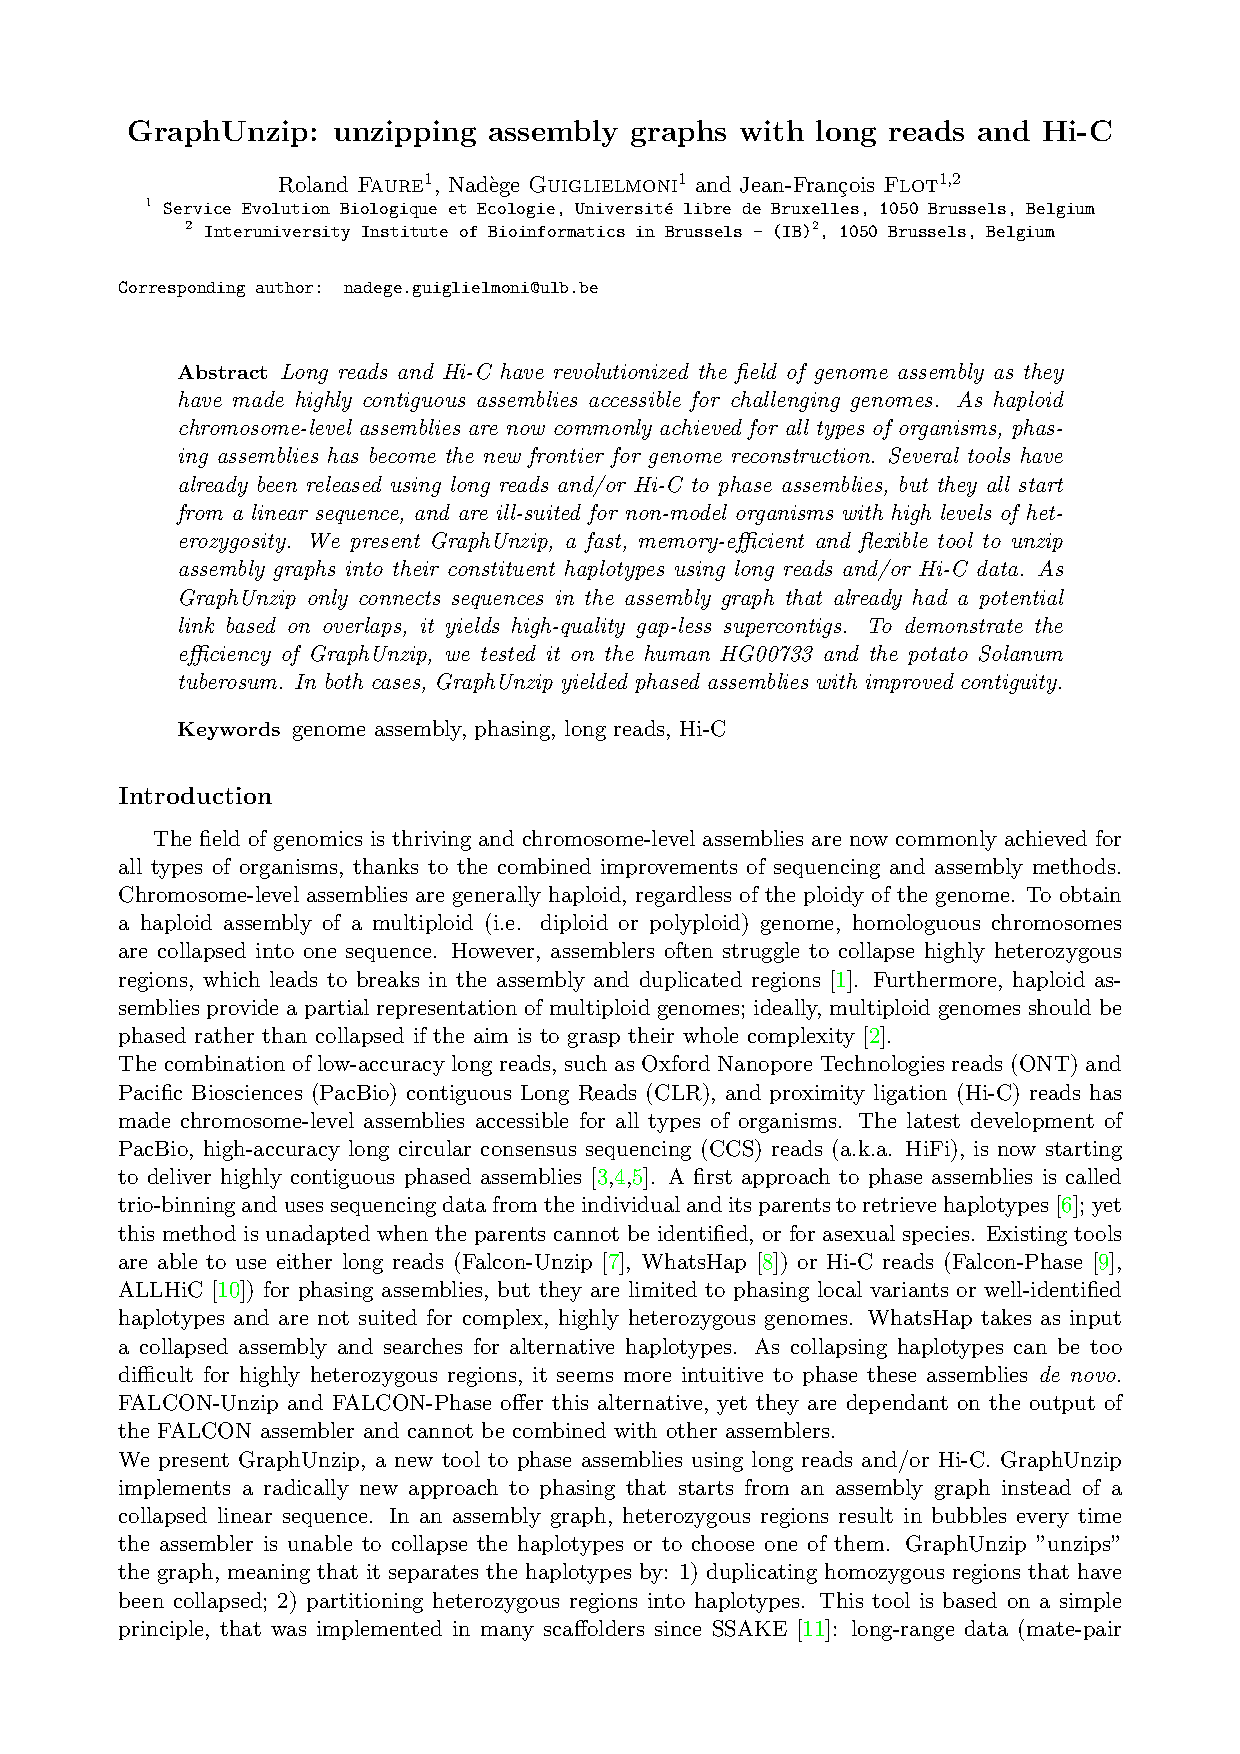
\includepdf[pages=-, pagecommand={}]{articles/graphunzip.pdf}

\textit{This chapter is a paper in preparation with Roland Faure (co-first author) and Jean-François Flot.}

\section{Introduction}

The field of genomics is thriving and chromosome-level assemblies are now commonly achieved for all types of organisms, thanks to the combined improvements of sequencing and assembly methods. Chromosome-level assemblies are generally haploid, regardless of the ploidy of the genome. To obtain a haploid assembly of a multiploid (i.e. diploid or polyploid) genome, homologuous chromosomes are collapsed into one sequence. However, assemblers often struggle to collapse highly heterozygous regions, which leads to breaks in the assembly and duplicated regions \cite{guiglielmoni2020}. Furthermore, haploid assemblies provide a partial representation of multiploid genomes; ideally, multiploid genomes should be phased rather than collapsed if the aim is to grasp their whole complexity \cite{unzipping}.\\

The combination of low-accuracy long reads, such as Oxford Nanopore Technologies reads (ONT) and Pacific Biosciences CLR, and proximity ligation (Hi-C) reads has made chromosome-level assemblies accessible for all types of organisms. The latest development of PacBio, high-accuracy long circular consensus sequencing (CCS) reads (a.k.a. HiFi), is now starting to deliver highly contiguous phased assemblies \cite{flye,hifiasm,hicanu}. A first approach to phase assemblies is called trio-binning and uses sequencing data from the individual and its parents to retrieve haplotypes \cite{triocanu}; yet this method is unadapted when the parents cannot be identified, or for asexual species. Existing tools are able to use either long reads (Falcon-Unzip \cite{falcon-unzip}, WhatsHap \cite{whatshap}) or Hi-C reads (Falcon-Phase \cite{falcon-phase}, ALLHiC \cite{allhic}) for phasing assemblies, but they are limited to phasing local variants or well-identified haplotypes and are not suited for complex, highly heterozygous genomes. WhatsHap takes as input a collapsed assembly and searches for alternative haplotypes. As collapsing haplotypes can be too difficult for highly heterozygous regions, it seems more intuitive to phase these assemblies \textit{de novo}. FALCON-Unzip and FALCON-Phase offer this alternative, yet they are dependant on the output of the FALCON assembler and cannot be combined with other assemblers. \\

We present GraphUnzip, a new tool to phase assemblies using long reads and/or Hi-C. GraphUnzip implements a radically new approach to phasing that starts from an assembly graph instead of a collapsed linear sequence. In an assembly graph, heterozygous regions result in bubbles every time the assembler is unable to collapse the haplotypes or to choose one of them. GraphUnzip "unzips" the graph, meaning that it separates the haplotypes by: 1) duplicating homozygous regions that have been collapsed; 2) partitioning heterozygous regions into haplotypes. This tool is based on a simple principle, that was implemented in many scaffolders since SSPACE \cite{sspace}: long-range data (mate-pair reads, long reads, proximity ligation...) give information on the linkage between contigs that can be used to group and orient them into scaffolds. As it takes as input and produces as output an assembly graph, our tool only connects contigs that are actually adjacent in the genome and yields gap-less scaffolds, i.e. supercontigs. GraphUnzip is compatible with any assembler that produces an assembly graph. We tested GraphUnzip on the genomes of the human HG00733 and the potato \textit{Solanum tuberosum}. GraphUnzip is available at \href{https://github.com/nadegeguiglielmoni/GraphUnzip}{github.com/nadegeguiglielmoni/GraphUnzip}. \\

\section{Methods}

\subsection{Inputs}

GraphUnzip requires an assembly graph in GFA format. The Hi-C input is a sparse matrix, such as the one obtained when processing the reads with hicstuff \cite{hicstuff}. Long reads are mapped to the assembly graph using GraphAligner \cite{graphaligner}.

\subsection{Overview of GraphUnzip}

In an assembly graph, contigs (segments) that are inferred to be adjacent or overlap in the assembly are connected with edges. However, some of these connections between contigs may be artefacts. To discriminate correct links from erroneous ones, GraphUnzip relies on long reads and/or Hi-C data. These data are translated to interactions between segments: two segments have a strong interaction based on long reads when many reads bridge both segments; strong Hi-C interactions correspond to frequent Hi-C contacts between the two segments. \\

GraphUnzip first builds one or two interaction matrices, depending on whether long-read data, Hi-C data or both are provided (Figure \ref{principle}). GraphUnzip reviews all segments and their links. For each link, an interaction intensity value $i$ is computed based on long reads data; if no link can be categorically deleted based on this data, the intensity value is computed based on Hi-C data. \\

When assessing two putative links A-B and A-C between segments A, B and C, the respective strengths of these links are calculated as the number of contacts (long reads or Hi-C) exclusive to A and B vs. the number of contacts exclusive to A and C. For example, in the third step of Figure \ref{principle}, when trying to associate segment (a,b) to either (d,e) or (d',f), only the contacts between (a,b) and e and f are considered. Contacts between (a,b) and d are discarded because they are not exclusive: both segments adjacent to (a,b) contain d.\\

When one segment has more than one potential link to other segments, these links are compared in a pairwise fashion. This comparison is made using two user-provided thresholds: the rejection threshold $T_R$ and the acceptance threshold $T_A$, where $T_R < T_A$. Considering two links X and Y and their respective interaction values $i(X)$ and $i(Y)$, if $i(X) < i(Y)$: link Y is considered strong; if $i(X)/i(Y) < T_R$, then the link X is considered weak; else, if $T_R \le i(X)/i(Y) < T_A$, the link X is flagged as dubious. The link X is considered strong when $i(X)/i(Y) \ge T_A$. The algorithm will consider thereafter that weak links are artefacts and do not actually exist in the genome whereas strong links represent true connections. \\

Weak links are removed. Then, every segment that has more that one strong link and no dubious links at one end is duplicated as many times as there are strong links. These segments are typically collapsed homozygous regions that need to be present in several copies to be phased with each allele. Every copy of the duplicated segment keeps the links of the original segment at its other end. This entails that the duplication of segments creates many new links. \\

The links are iteratively processed to entirely phase the assembly for $s$ steps, where $s$ is a user-provided parameter. Because extremely long segments tend to share a significant number of Hi-C contacts even if they are not adjacent, we observed that in extreme cases the algorithm could join two chromosomes by their telomeric ends. The Hi-C matrix is used at the end of the process to detect such chimeric connections in the assembly graph, based on low Hi-C interactions, and break them. \\

\begin{figure}
    \centering
    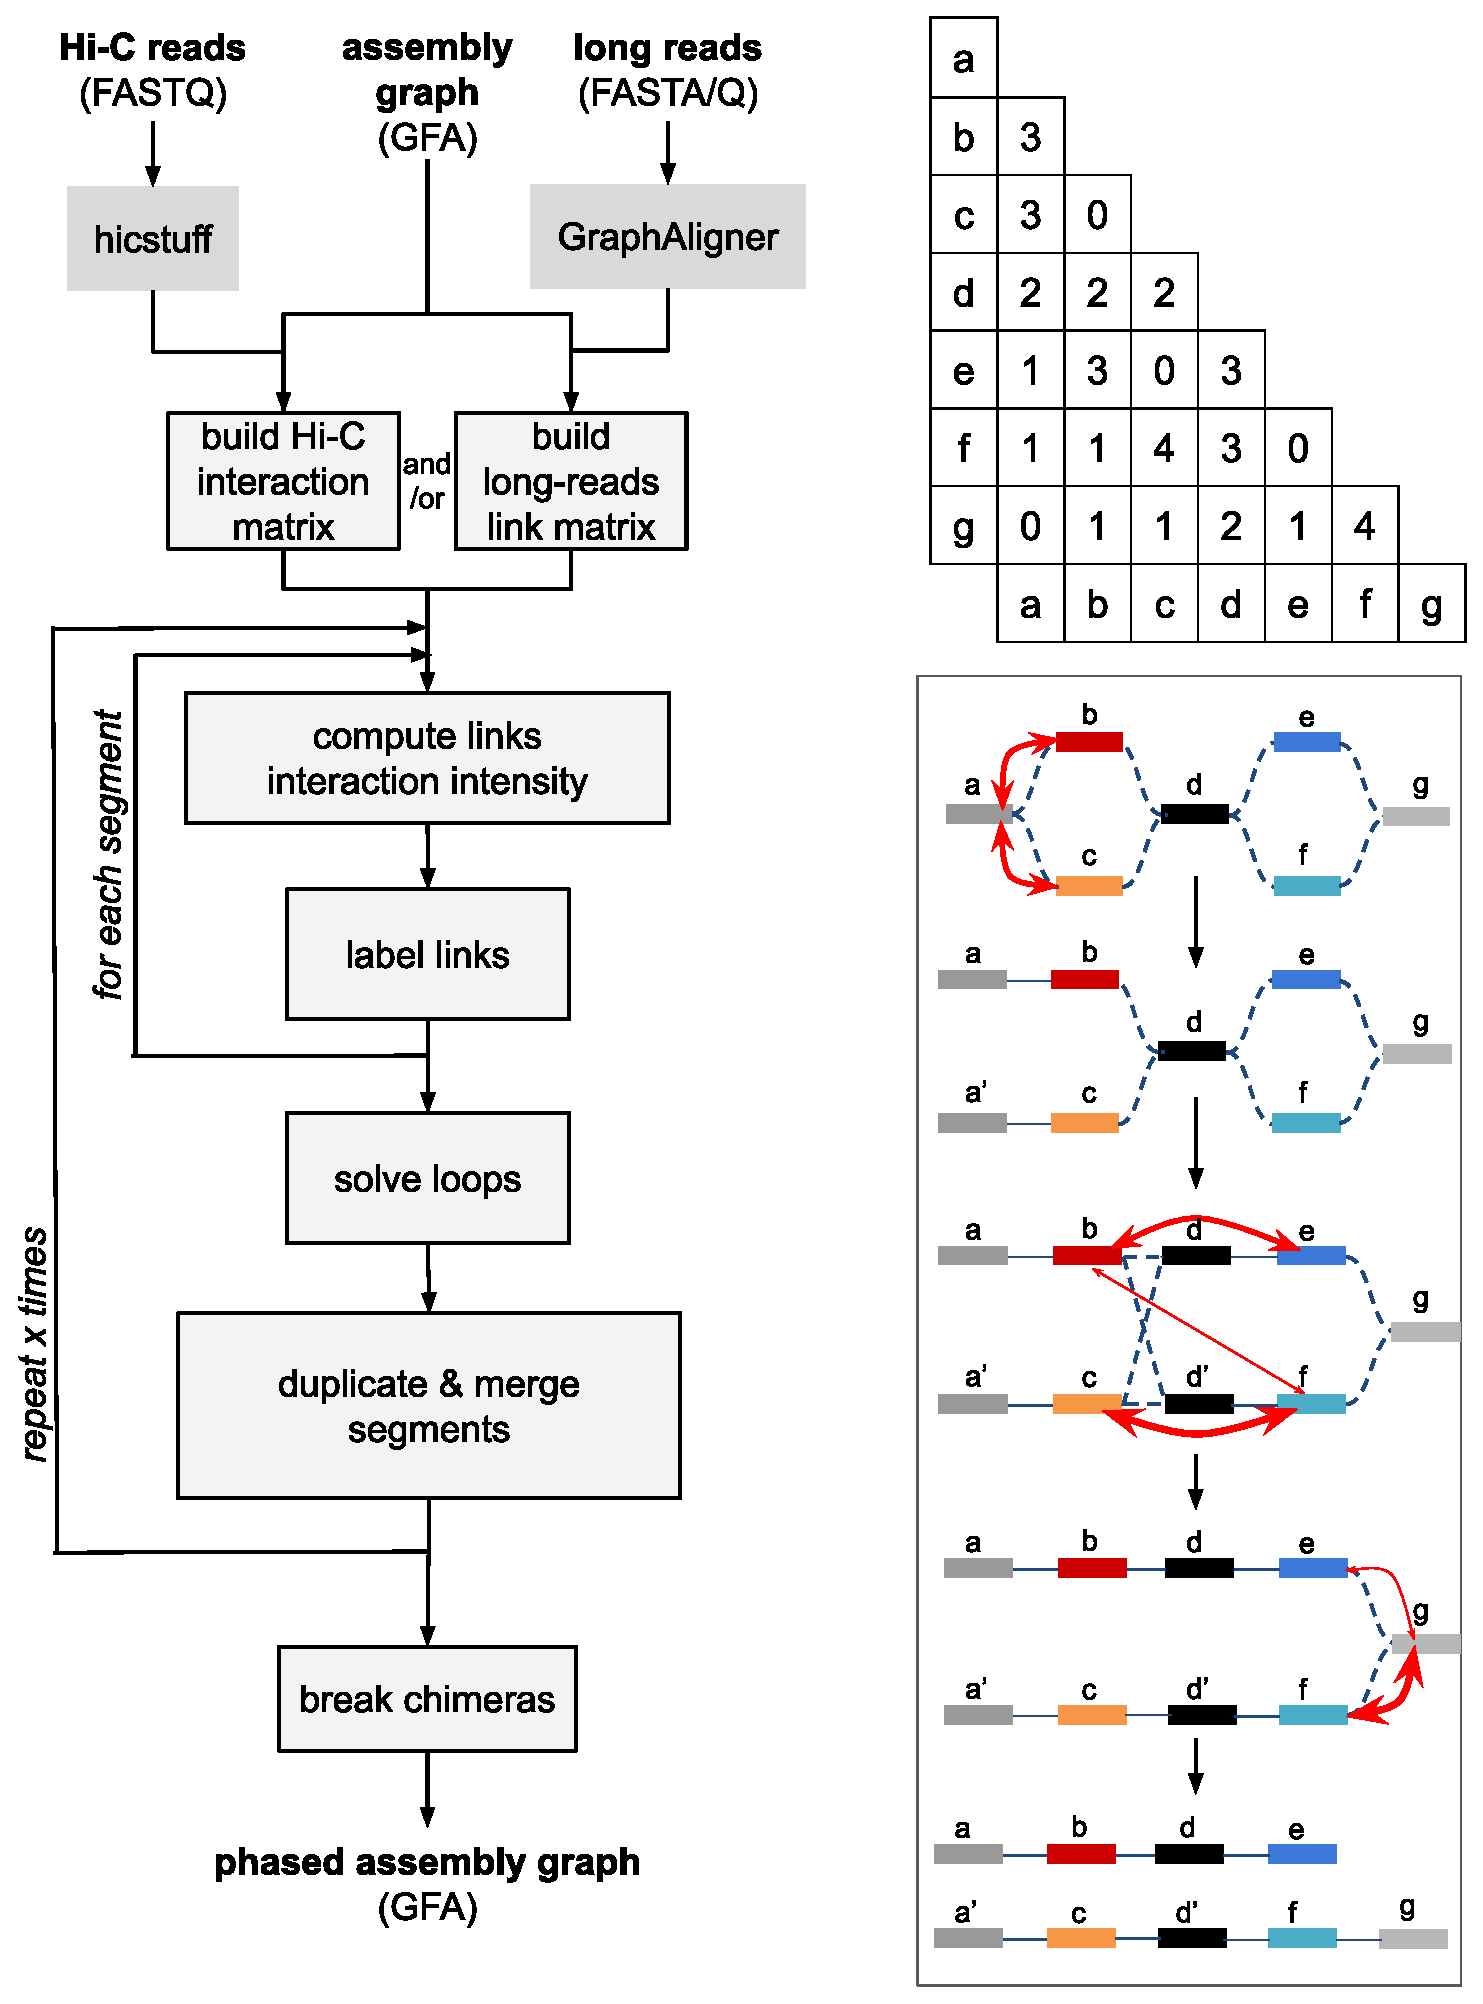
\includegraphics[width=16cm]{fig/graphunzip_description.eps}
    \caption{\label{principle} Description of GraphUnzip: workflow of the program (left), interaction matrix (top right), and overview of the algorithm to discriminate links (bottom right). This example algorithm analyzes the potential links between the segments a, b, c, d, e, f, g. The red arrows represent the intensity of interactions between the segments, computed based on the values in the matrix.}
\end{figure}

\subsection{\textit{Homo sapiens} HG00733 assemblies}

Reads were published in \cite{phased_human}. The HiFi reads were assembled with hifiasm with the parameter \texttt{-l 0}, and we then used the p\_utg assembly graph. All the HiFi reads and the ONT reads longer than 30 kb were mapped to the assembly using GraphAligner with the parameter \texttt{-x vg}. Hi-C reads were processed with hicstuff using the parameters \texttt{-{}-aligner bowtie2 -{}-enzyme 200 -{}-iterative}. GraphUnzip was run with parameters \texttt{--accept 0.10 --reject 0.05 -{}-exhaustive -{}-whole\_match -{}-minimum\_match 0.8}. All non-ambiguous paths in the GFA were merged with Bandage. The assemblies were compared to the DipAsm reference \cite{dipasm} using QUAST v5.0.2 \cite{quast} with the parameters \texttt{-m 0 --eukaryote --large --min-identity 99.9}.

\subsection{\textit{Solanum tuberosum} assemblies}

Reads published in \cite{potato} were retrieved from the NCBI Sequence Read Archive with the Bioproject accession number PRJNA573826. The HiFi reads were assembled with hifiasm with the parameter \texttt{-l 0}, and we then used the p\_utg assembly graph. All the HiFi reads and the ONT reads longer than 25 kb were mapped to the assembly using GraphAligner with the parameter \texttt{-x vg}. Hi-C reads were processed with hicstuff using the parameters \texttt{-{}-aligner bowtie2 -{}-enzyme MboI -{}-iterative}. GraphUnzip was run with parameters \texttt{--accept 0.40 --reject 0.10 -{}-exhaustive -{}-whole\_match -{}-minimum\_match 0.8}. All non-ambiguous paths in the GFA were merged with Bandage. To check the output of GraphUnzip, we mapped the published assembly to the assembly graph using GraphAligner. We used calN50 available at \href{https://github.com/lh3/calN50}{github.com/lh3/calN50} to compute NG50, against a size of 1.67 Gb (published assembly size \cite{potato}). BUSCO v4 \cite{busco_evaluation} was run with parameters \texttt{-m genome --long} against the dataset viridiplantae odb10. 

\subsection{Computational performance}

RAM usage and CPU time were measured with the command \texttt{/usr/bin/time -v} on a desktop computer with 128 GB of RAM and a i9-9900X 3.5 GHz processor.

\section{Results}

\subsection{\textit{Homo sapiens} HG00733}

\begin{table*}[ht]
    \begin{center}
    \caption{\label{tab:homo_sapiens_assemblies}Assembly metrics of \textit{Homo sapiens} HG00733 compared with the DipAsm reference.}
    \begin{tabular}{llcccccc}
        \hline
        \textbf{Assembly} & \textbf{GraphUnzip} & \textbf{Size} & \textbf{N50} & \textbf{NA50} & \textbf{Misassemblies} & \textbf{CPU} & \textbf{RAM} \\
        \hline
        Reference & - & 5.9 Gb & 27.8 Mb & 27.8 Mb & 84 & - & - \\
        \hline
        hifiasm & - & 5.5 Gb & 397 kb & 343 kb & 9146 & - & - \\
            & ONT + Hi-C & 6.2 Gb & 1.5 Mb & 1.2 Mb & 8091 & 33min 46s & 23.5 GB \\
        \hline
        \end{tabular}
  \end{center}
\end{table*}

We compared the hifiasm + GraphUnzip assembly of the human HG00733 genome with a published reference obtained with DipAsm. GraphUnzip increased the size of the hifiasm assembly (from 5.5 Gb to 6.2 Gb), and the N50 rose as well (from 397 kb to 1.2 Mb) (Table \ref{tab:homo_sapiens_assemblies}). The NA50 was improved while the number of misassemblies decreased in the GraphUnzip supercontigs. Notably, the reference assembly size is only 5.9 Gb, while the GraphUnzip assembly reaches 6.2 Gb, which is the expected size for a phased human genome. That is why we show the NA50s rather than the NGA50s. \\

We also tried an assembly of the HiFi reads with Flye, but the draft assembly was only 2.9 Gb, little below half the expected size, which indicates that the haplotypes were collapsed. A good candidate assembly for GraphUnzip should have uncollapsed heterozygous regions, as GraphUnzip is not able to retrieve a missing haplotype in collapsed heterozygous regions and can only duplicate the remaining haplotype, leading in that case to a suboptimal result.

\subsection{\textit{Solanum tuberosum}}

\begin{table*}[ht]
    \begin{center}
    \caption{\label{tab:solanum_tuberosum_assemblies}Assembly metrics of \textit{Solanum tuberosum}. The NG50 values were computed based on an estimated genome size of 1.67 Gb.}
    \begin{tabular}{llcccccc}
        \hline
        \multirow{2}{*}{\textbf{Assembly}} & \multirow{2}{*}{\textbf{GraphUnzip}} & \multirow{2}{*}{\textbf{Size}} & \multirow{2}{*}{\textbf{NG50}} &  \multicolumn{2}{c}{\textbf{BUSCO}} & \multirow{2}{*}{\textbf{CPU}} & \multirow{2}{*}{\textbf{RAM}} \\
        & & & & \textbf{Single} & \textbf{Dup.} & & \\
        \hline
        Reference & - & 1.67 Gb & 66.1 Mb & 21.6\% & 76.9\% & - & - \\
        \hline
        hifiasm & - & 1.51 Gb & 2.2 Mb & 21.2\% & 77.9\% & - & - \\
            & HiFi & 1.69 Gb & 3.7 Mb & 7.1\% & 91.5\% & 16s & 0.2 GB \\
            & ONT & 1.67 Gb & 3.4 Mb & 6.8\% & 92.2\% & 52s & 0.2 GB \\
            & Hi-C & 1.69 Gb & 5.6 Mb & 7.8\% & 91.5\% & 38min 27s & 11.5 GB\\
            & HiFi + Hi-C & 1.69 Gb & 4.9 Mb & 9.4\% & 89.4\% & 39min 59s & 11.5 GB \\
            & ONT + Hi-C & 1.73 Gb & 5.9 Mb & 7.3\% & 91.8\% & 39min 10s & 11.5 GB \\
        \hline
        \end{tabular}
  \end{center}
\end{table*}

We tested GraphUnzip on the diploid genome of the potato \textit{Solanum tuberosum} RH89-039-16, for which a phased assembly of 1.67 Gb \cite{potato} was recently published. We assembled the HiFi reads with hifiasm and then ran GraphUnzip using the HiFi, ONT and/or Hi-C reads. The draft assembly was 1.51 Gb, and after phasing with GraphUnzip, the assembly size rose to 1.67-1.73 Gb (Table \ref{tab:solanum_tuberosum_assemblies}). GraphUnzip also increased the contiguity: from 2.2 Mb, the NG50 reached 3.4 to 5.9 Mb. The combination of both ONT and Hi-C reads yielded the highest NG50. Hi-C reads improved the contiguity better than long reads. The overall BUSCO completeness of the GraphUnzip supercontigs is slightly higher than the reference: 98.6-99.3\% against 98.5\% for the reference, and the number of duplicated BUSCO features is higher as well (89.4-92.2\% against 76.9\%). We mapped the published assembly to the GraphUnzip assembly graph obtained when using Hi-C and ONT reads. We found that there were no differences in phasing between the two assemblies. However, some regions that were phased by hifiasm and GraphUnzip were collapsed in the published assembly. This result, in conjunction with the higher number of duplicated features, indicates that GraphUnzip led to an improved phased assembly. \\

\subsection{Computational performance}

For both the human genome and \textit{Solanum tuberosum} genome, GraphUnzip required limited computational resources, as it ran in less than 1 hour on a single thread and used up to 23.5 GB of memory. For \textit{Solanum tuberosum}, the run time was also shorter when using only long reads, below 1 minute. The longer run time when using Hi-C reads was due to the building of the interaction matrix. As this interaction matrix is outputted by the program, this file can be reused for other runs, that will finish faster. Therefore, users can try several sets of parameters to optimize the result, with short runtimes. \\

\section{Conclusion}

GraphUnzip is a flexible tool that can phase assemblies of high-accuracy long reads with long reads and/or Hi-C. A limitation of GraphUnzip is that it does not necessarily reach chromosome-level assemblies like most Hi-C scaffolders, but it aims instead to produce more contiguous gap-less supercontigs by fully exploiting assembly graphs. As genome projects now usually include long reads and Hi-C to obtain chromosome-level assemblies, GraphUnzip can easily be integrated in assembly projects to obtain \textit{de novo} phased assemblies for non-model organisms. \\

% write your paper in here

\chapter{Scaffolding assemblies with Hi-C}

Recent genome assembly projects generally aim to achieve chromosome-level scaffolds, and Hi-C scaffolding is a major step to reach this goal. This method has been included successfully in many studies for bacteria, yeasts, plants, animals, and is part of assembly pipelines for several consortia, such as the Vertebrate Genome Project \cite{vgp} and the Darwin Tree of Life \cite{dtol}. instaGRAAL is an overhauled, improved version of GRAAL \cite{graal}, a Hi-C scaffolder inspired by Gibbs sampling, a MCMC-based approach, to iteratively test and ponder arrangements of DNA fragments until the resulting organization converges towards an assembly with a higher likelihood based on contact frequencies. Two main aspects were improved: first, instaGRAAL, through the use of sparse contact maps, is more computationally efficient, enabling it to handle larger genomes (over 1 Gb); second, it introduces a module to automatically refine the scaffolds based on the input contigs, and reduce local misassemblies. In the following paper, instaGRAAL was used to assemble the brown algae \textit{Desmarestia herbacea} and \textit{Ectocarpus} sp., and benchmarked against SALSA2 \cite{salsa2} on a human; it systematically yielded chromosome-level scaffolds. \\
I contributed to testing instaGRAAL, in particular regarding its application to the human genome. I also improved the documentation to make it more accessible for new users, and contribute since then to the maintenance of the program on the github account of Romain Koszul's lab  \href{https://github.com/koszullab/instaGRAAL}{github.com/koszullab/instaGRAAL}. \\

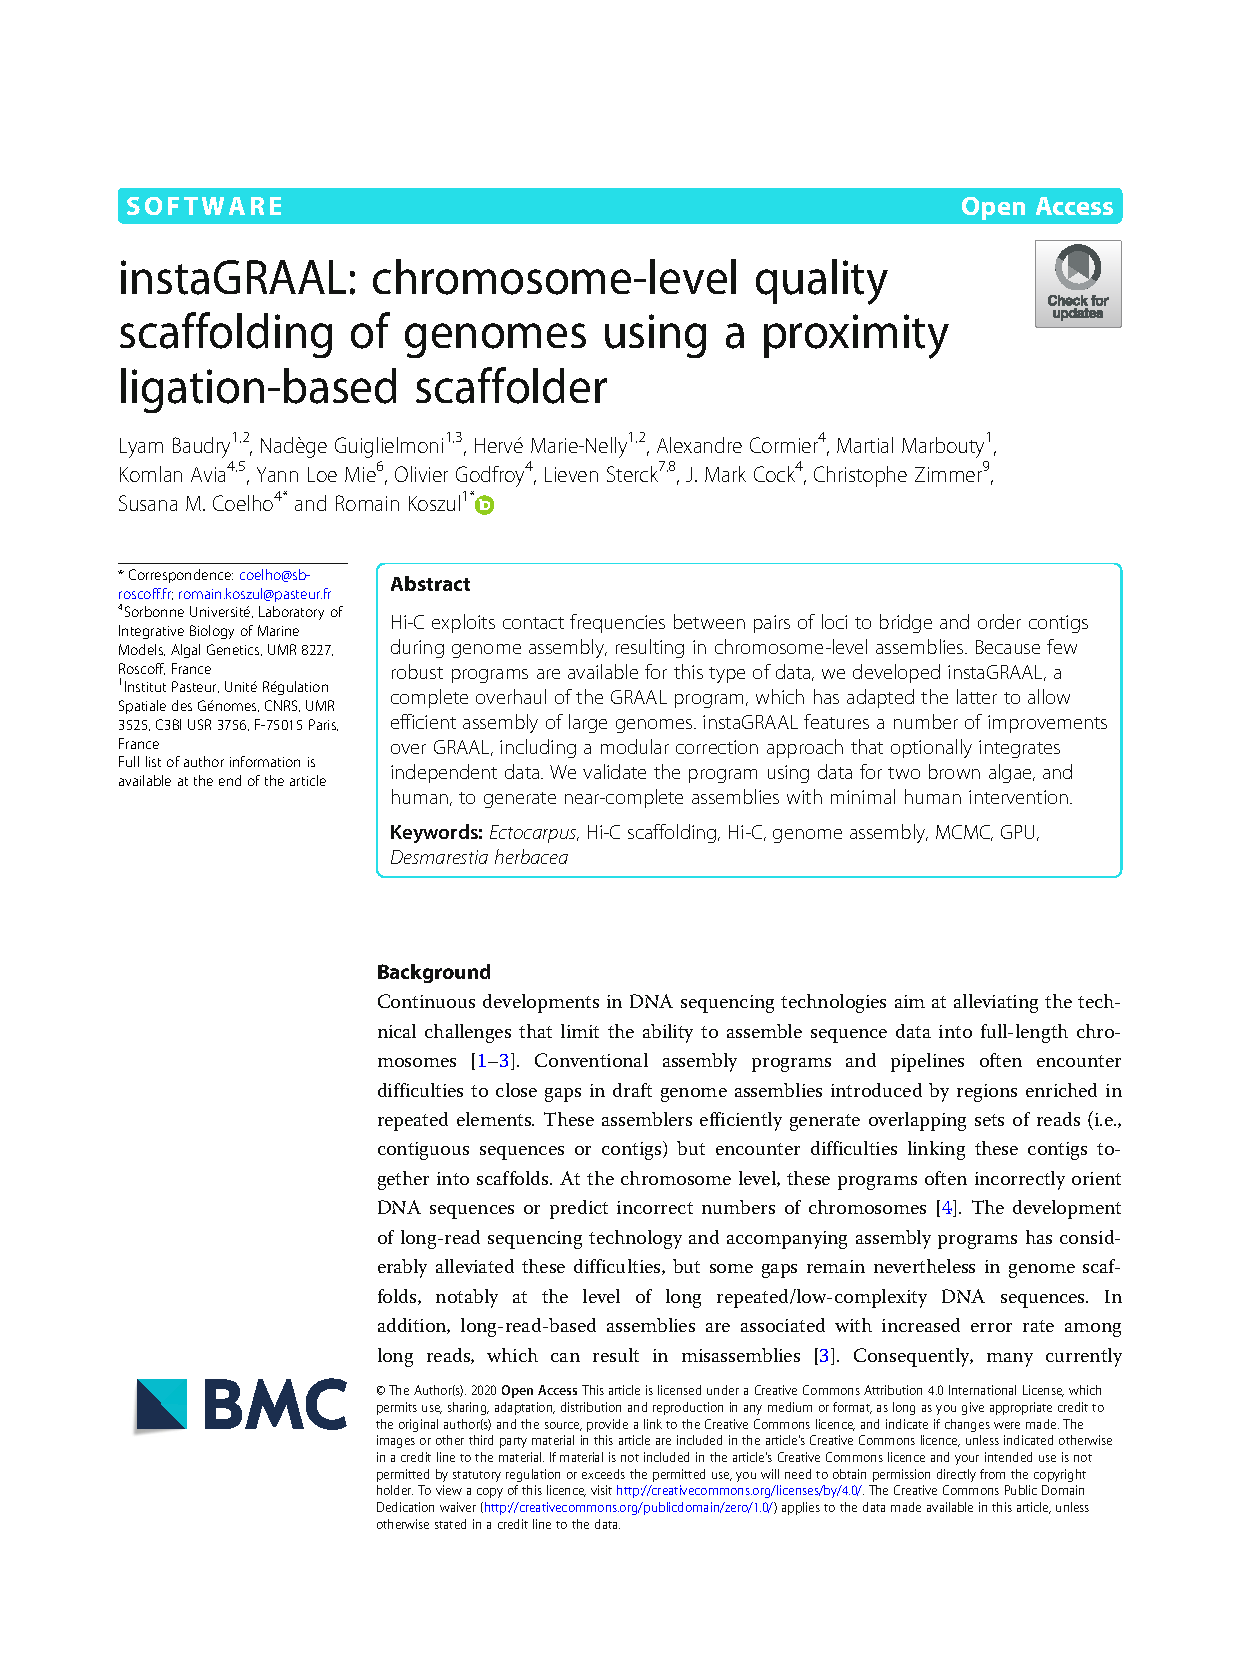
\includepdf[pages=-, pagecommand={}]{articles/instagraal.pdf}

\begin{suppsection}
\beginsupplement

\begin{table}[ht]
\centering
\caption{Example of a sparse matrix.}
\begin{tabular}{|c|c|c|}
\hline
\textbf{id\_frag\_a} & \textbf{id\_frag\_b} & \textbf{n\_contacts} \\
\hline
0 & 0 & 1368 \\
0 & 1 & 21 \\
0 & 2 & 7 \\
0 & 3 & 3 \\
0 & 4 & 5 \\
0 & 7 & 5 \\
0 & 8 & 1 \\
0 & 9 & 1 \\
0 & 12 & 2 \\
0 & 15 & 1 \\
0 & 22 & 1 \\
0 & 23 & 1 \\
0 & 26 & 1 \\
0 & 27 & 1 \\
0 & 33 & 2 \\
0 & 36 & 2 \\
0 & 37 & 1 \\
0 & 51 & 1 \\
0 & 69 & 1 \\
0 & 74 & 2 \\
0 & 76 & 1 \\
0 & 97 & 1 \\
0 & 99 & 1 \\
0 & 107 & 1 \\
\hline
\end{tabular}
\label{tab:t1}
\end{table}

\begin{table}[ht]
\centering
\caption{Comparison of the integrated sequences between the different assemblies and the v1 assembly for \textit{Ectocarpus} sp.}
\begin{tabular}{|l|c|c|c|}
\hline
    & \textbf{v1 assembly} & \textbf{linkage group} & \textbf{corrected instaGRAAL} \\
    &  & \textbf{v2 assembly} & \textbf{v4 assembly} \\
\hline
Scaffolds integrated into linkage & 325 & 531 & 793 \\
groups (out of 1561) &  &  &  \\
\hline
Percent sequence data integrated & 70.10\% & 90.50\% & 96.80\% \\
into linkage groups &  &  &  \\
\hline
Integrated oriented scaffolds in & 12\% & 49\% & 100\% \\
the linkage groups &  &  &  \\
\hline
Number of linkage groups & 34 & 28 & 27 \\
\hline
\end{tabular}
\label{tab:t2}
\end{table}

\begin{table}[ht]
\centering
\caption{Correspondences between instaGRAAL super scaffolds and linkage groups from the v2 assembly for the \textit{Ectocarpus} sp. genome.}
\begin{tabular}{|c|c|}
\hline
\textbf{instaGRAAL} & \textbf{Linkage group} \\
\textbf{v4 assembly} & \textbf{v2 assembly} \\
\hline
1 & 1 \\
2 & 21 \\
3 & 4 \& 28 \\
4 & 5 \\
5 & 13 \\
6 & 6 \\
7 & 12 \\
8 & 7 \\
9 & 27 \\
10 & 26 \\
11 & 3 \\
12 & 2 \\
13 & 8 \\
14 & 14 \\
15 & 10 \\
16 & 11 \\
17 & 19 \\
18 & 16 \\
19 & 9 \\
20 & 15 \\
21 & 18 \\
22 & 20 \\
23 & 24 \\
24 & 23 \\
25 & 17 \\
26 & 25 \\
27 & 22 \\
\hline
\end{tabular}
\label{tab:t3}
\end{table}

\begin{table}[ht]
\centering
\caption{Metrics of \textit{Desmarestia herbacea} assemblies using three different programs.}
\begin{tabular}{|l|c|c|c|c|}
\hline
    & \textbf{\textit{De novo} original assembly} & \textbf{3D-DNA} & \textbf{SALSA2} & \textbf{instaGRAAL} \\
\hline
N50 (bp) & 184,092 & 175,000 & 12,780,148 & 12,444,485 \\
L50 & 697 & 545 & 11 & 17 \\
Contig count & 7,743 & 5,385 & 4,827 & 4,304 \\
BUSCO \% & 72.6 & 70.7 & 73.6 & 73.0 \\
\hline
\end{tabular}
\label{tab:t4}
\end{table}

\begin{table}[ht]
\centering
\caption{Performance of GRAAL and instaGRAAL at scaffolding the \textit{Ectocarpus} sp. genome. }
\begin{tabular}{|l|c|c|}
\hline
    & \textbf{GRAAL} & \textbf{instaGRAAL} \\
\hline
Peak memory load (Gb) & 2.5 & 1.1 \\
Memory used in graphic card & 113 (Mb) & 11 \\
Per-cycle runtime (avg. over 20 min) & 13 & 4 \\
\hline
\end{tabular}
\label{tab:t5}
\end{table}

\begin{figure}[ht]
\centering
    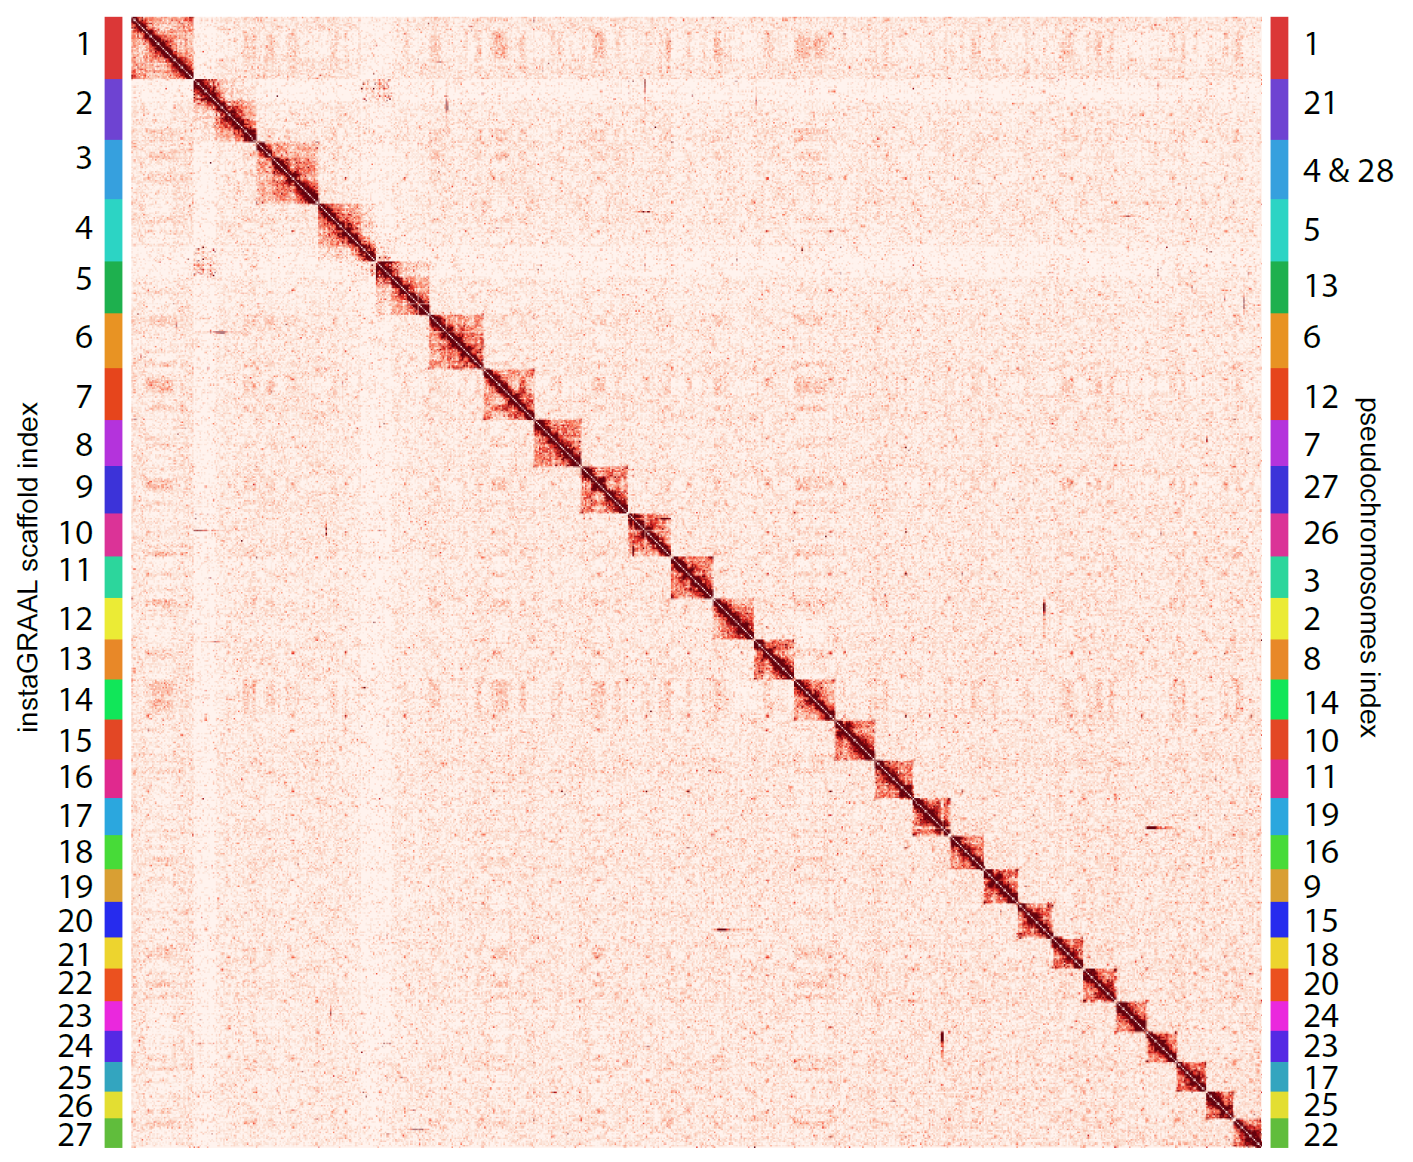
\includegraphics[width=13.5cm]{fig/instagraal/s1.png}
    \caption{Normalized contact map of the \textit{Ectocarpus} sp. genome scaffolded using instaGRAAL (bin = 200 kb). The colour scale represents the normalized interaction frequencies. No large-scale rearrangements are clearly apparent in the interchromosomal contacts. On the right the linkage groups indices from the v2 assembly are indicated.}
    \label{fig:instagraal_s1}
\end{figure}

\begin{figure}[ht]
\centering
    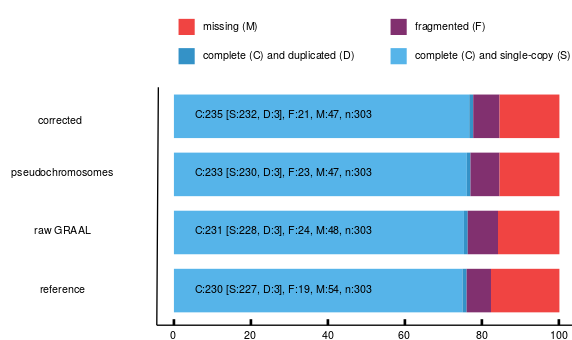
\includegraphics{fig/instagraal/s2.png}
    \caption{Estimates of BUSCO completeness for the three \textit{Ectocarpus} sp. assemblies and the reference genome v1 assembly.}
    \label{fig:instagraal_s2}
\end{figure}

\begin{figure}[ht]
\centering
    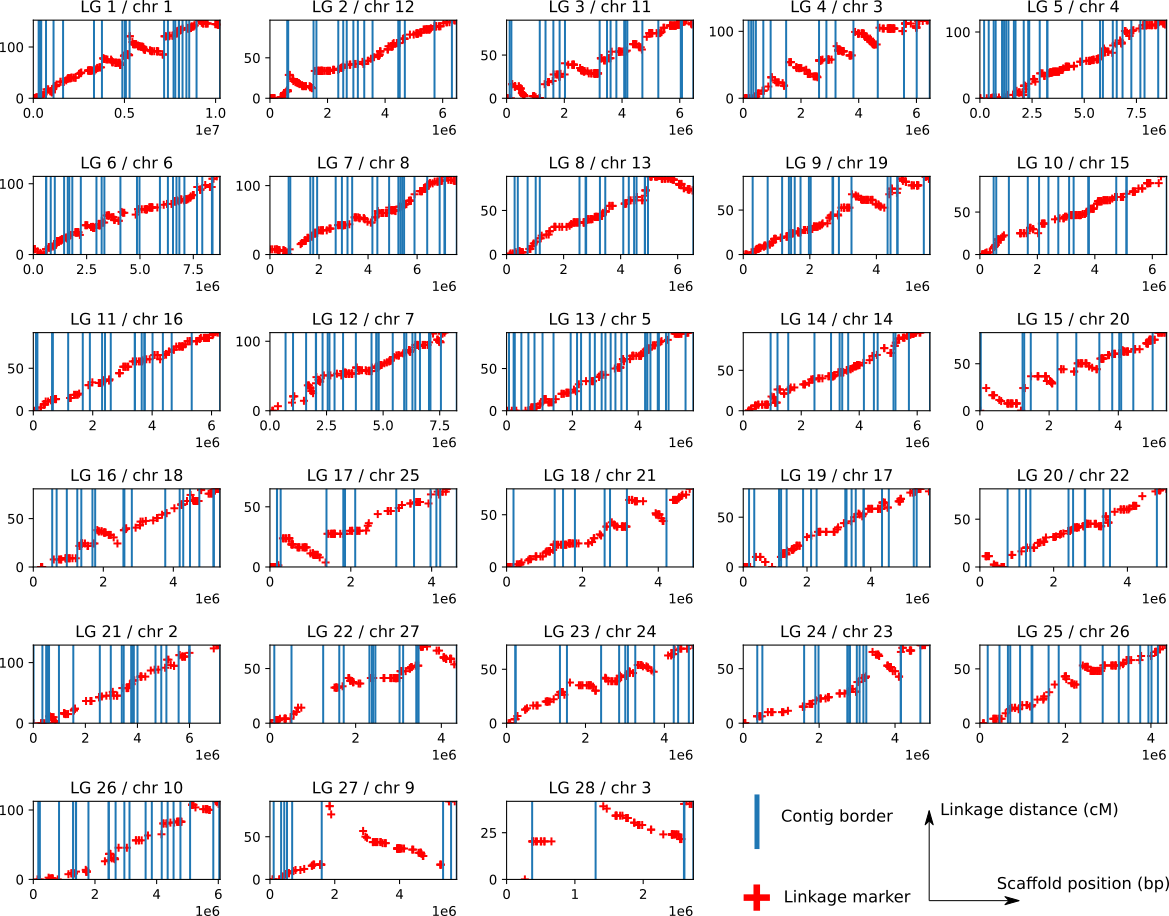
\includegraphics[width=13.5cm]{fig/instagraal/s3.png}
    \caption{Linkage markers vs. scaffold positions for all linkage groups/chromosomes (chromosome 3 is made up of linkage groups 4 and 28). The initial contig borders within each chromosome have been underlined. Linkage marker positions are always monotonous (only increasing, or only decreasing) within an initial contig.}
    \label{fig:instagraal_s3}
\end{figure}

\begin{figure}[ht]
\centering
    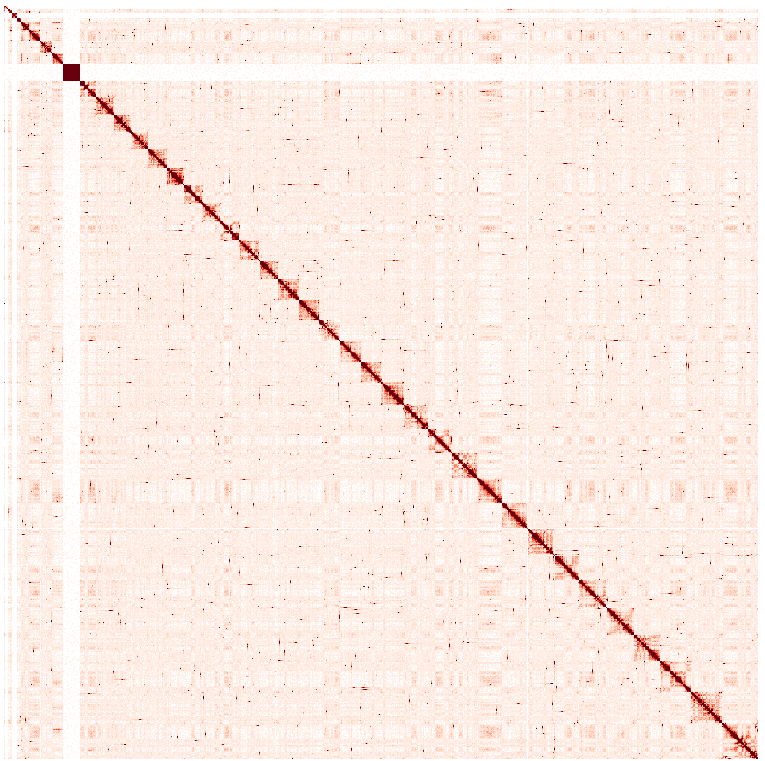
\includegraphics[width=13.5cm]{fig/instagraal/s4.png}
    \caption{The 40 main scaffolds of \textit{Desmarestia herbacea} after instaGRAAL scaffolding.}
    \label{fig:instagraal_s4}
\end{figure}

\begin{figure}[ht]
\centering
    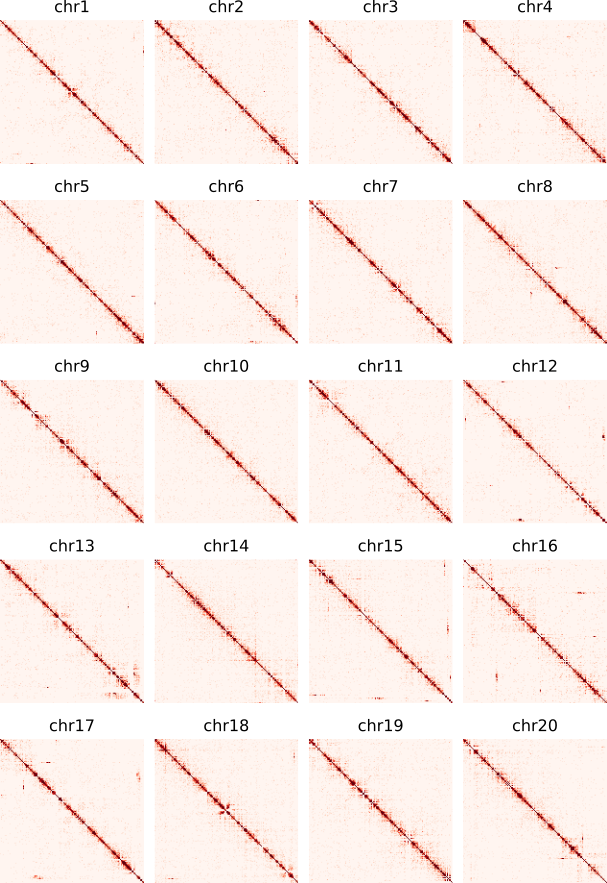
\includegraphics[width=13.5cm]{fig/instagraal/s5.png}
    \caption{Contact maps of the first twenty newly formed scaffolds/putative chromosomes of \textit{Desmarestia herbacea}, generated after scaffolding at a 20-kb resolution.}
    \label{fig:instagraal_s5}
\end{figure}

\begin{figure}[ht]
\centering
    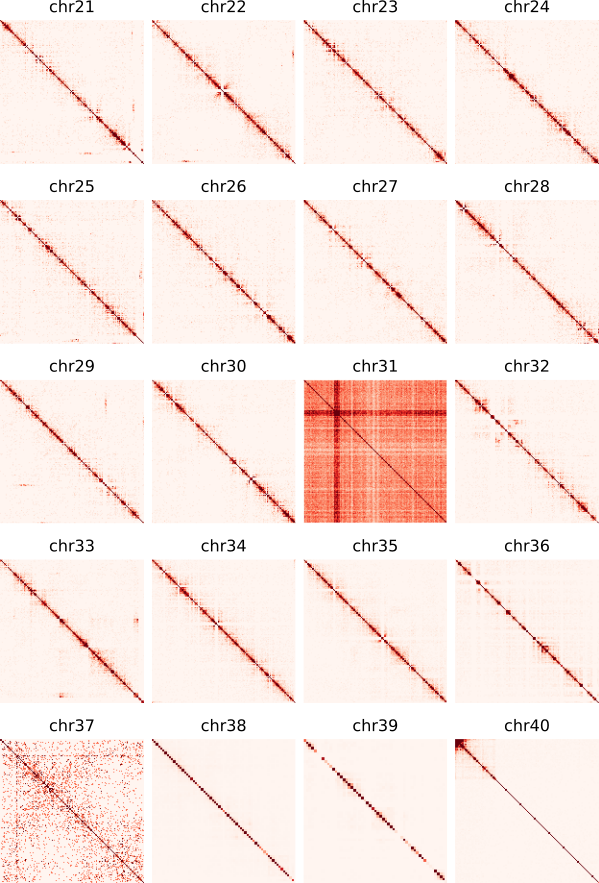
\includegraphics[width=13.5cm]{fig/instagraal/s6.png}
    \caption{The last twenty newly formed scaffolds/putative chromosomes of \textit{Desmarestia herbacea} post-scaffolding at a 20-kb resolution.}
    \label{fig:instagraal_s6}
\end{figure}

\begin{figure}[ht]
\centering
    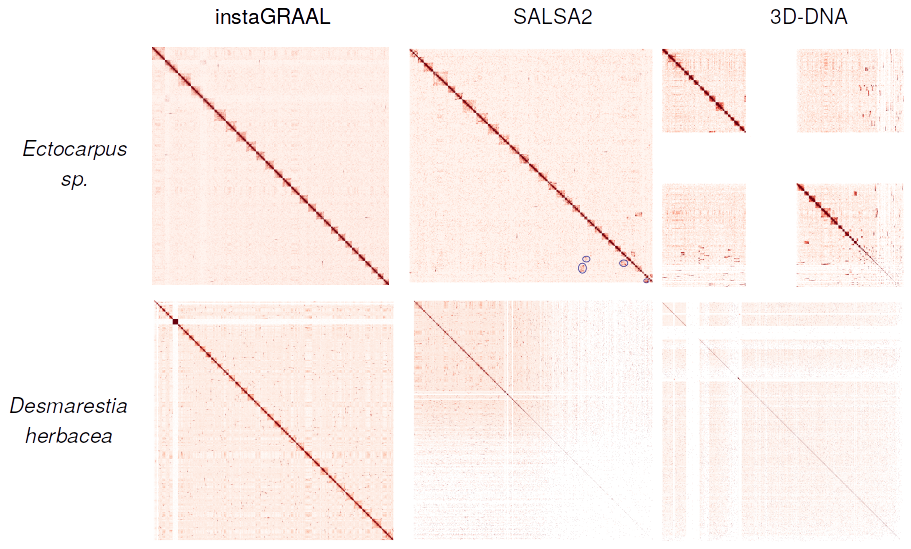
\includegraphics[width=13.5cm]{fig/instagraal/s7.png}
    \caption{Normalized contact map of the \textit{Ectocarpus} sp. genome scaffolded using instaGRAAL (bin = 200 kb). The colour scale represents the normalized interaction frequencies. No large-scale rearrangements are clearly apparent in the interchromosomal contacts. On the right the linkage groups indices from the v2 assembly are indicated.}
    \label{fig:instagraal_s7}
\end{figure}

\begin{figure}[ht]
\centering
    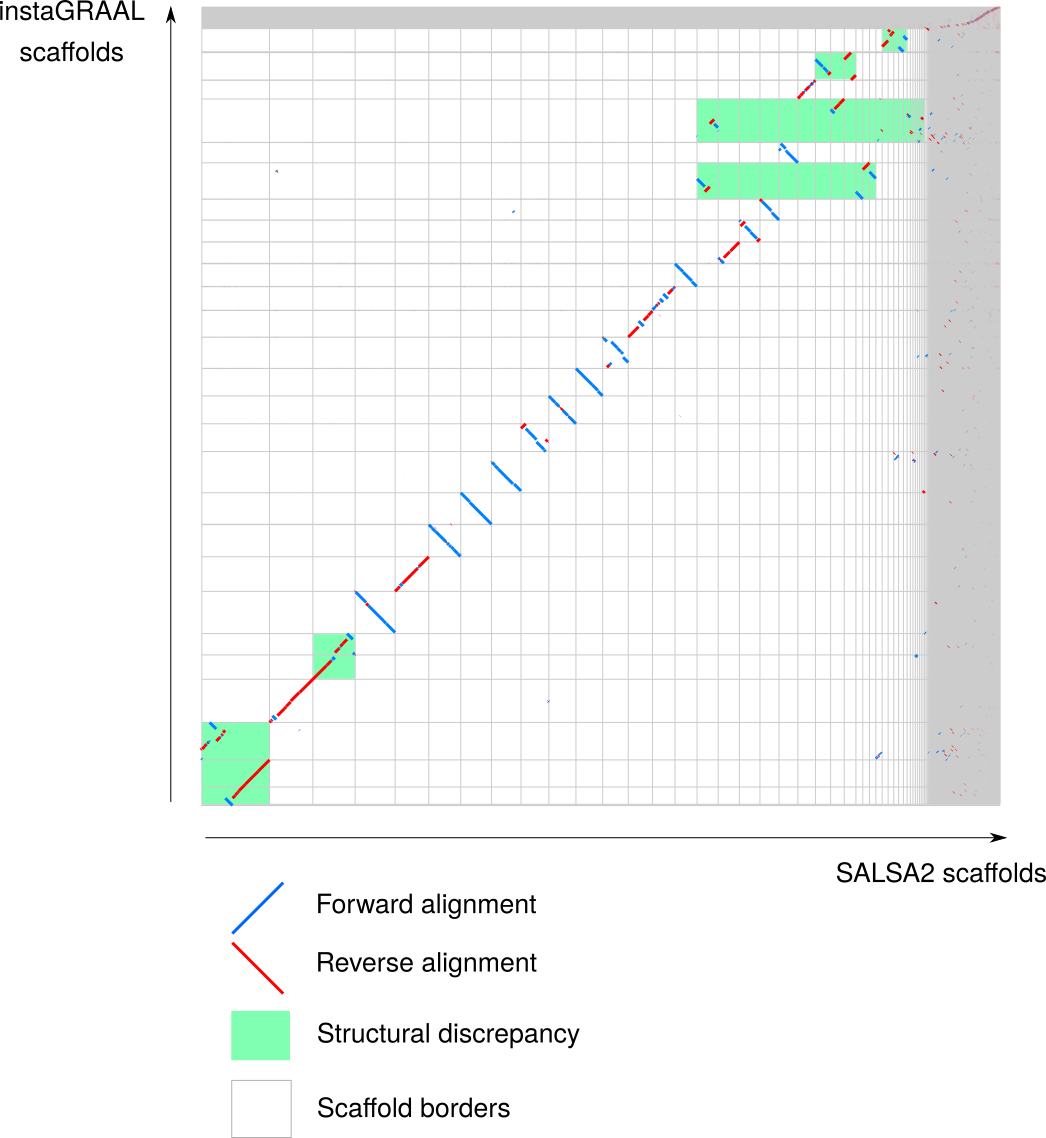
\includegraphics[width=13.5cm]{fig/instagraal/s8.png}
    \caption{Similarity dotplot of the SALSA2 vs. instaGRAAL 27 scaffolds for \textit{Ectocarpus} sp. large-scale structural discrepancies have been underlined in green. The contact maps suggest instaGRAAL solutions are more likely. }
    \label{fig:instagraal_s8}
\end{figure}

\begin{figure}[ht]
\centering
    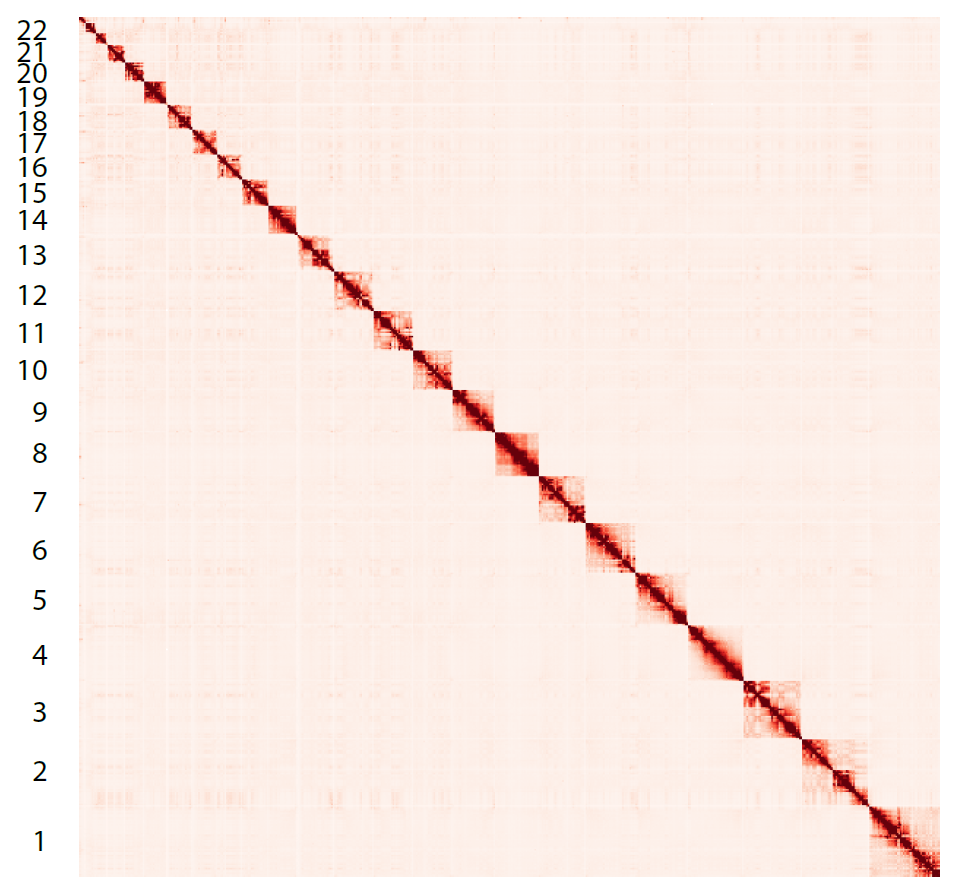
\includegraphics[width=13.5cm]{fig/instagraal/s9.png}
    \caption{Contact map of the \textit{Homo sapiens} genome, fragmented in 300 kb sequences, after scaffolding with instaGRAAL, at 5-Mb resolution.}
    \label{fig:instagraal_s9}
\end{figure}

\begin{figure}[ht]
\centering
    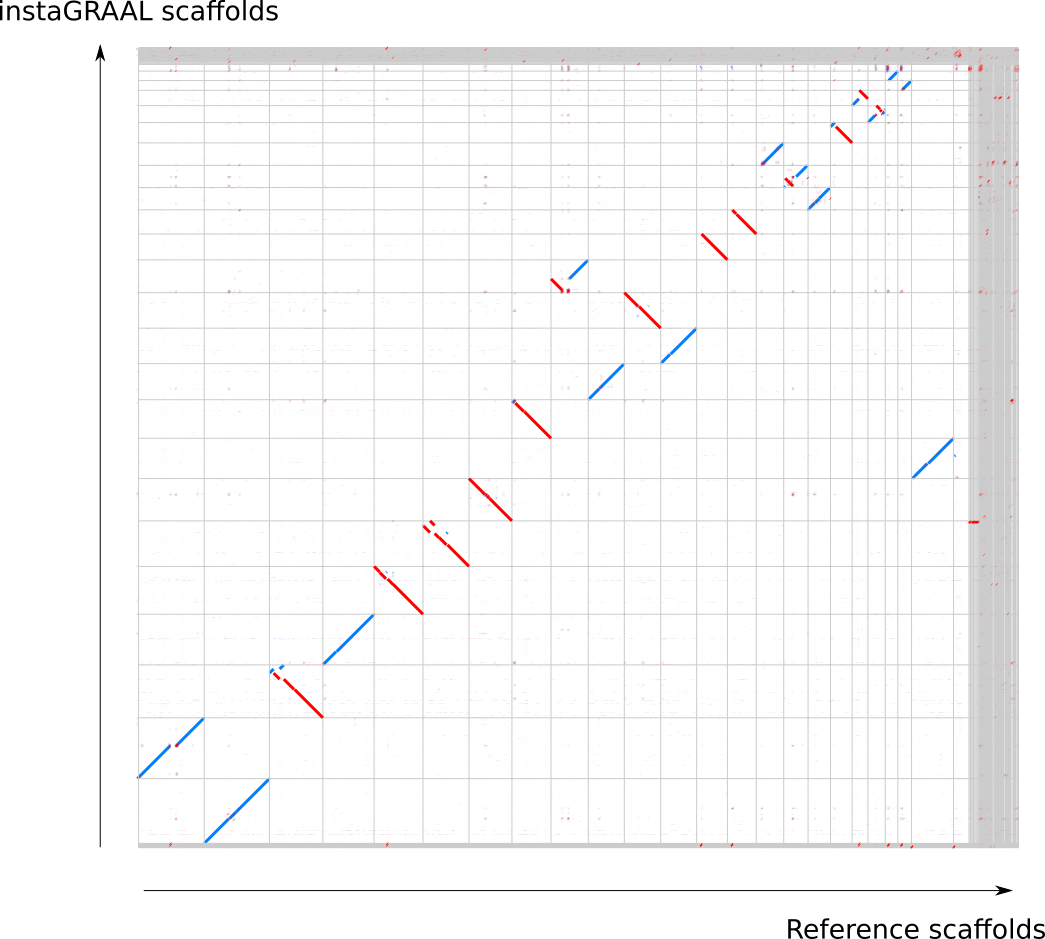
\includegraphics[width=13.5cm]{fig/instagraal/s10.png}
    \caption{Similarity dotplot of the instaGRAAL vs. reference scaffolds for the GRCh38 human genome. Relocations are visible but the one-to-one mapping between the 23 first scaffolds is preserved.}
    \label{fig:instagraal_s10}
\end{figure}

\begin{figure}[ht]
\centering
    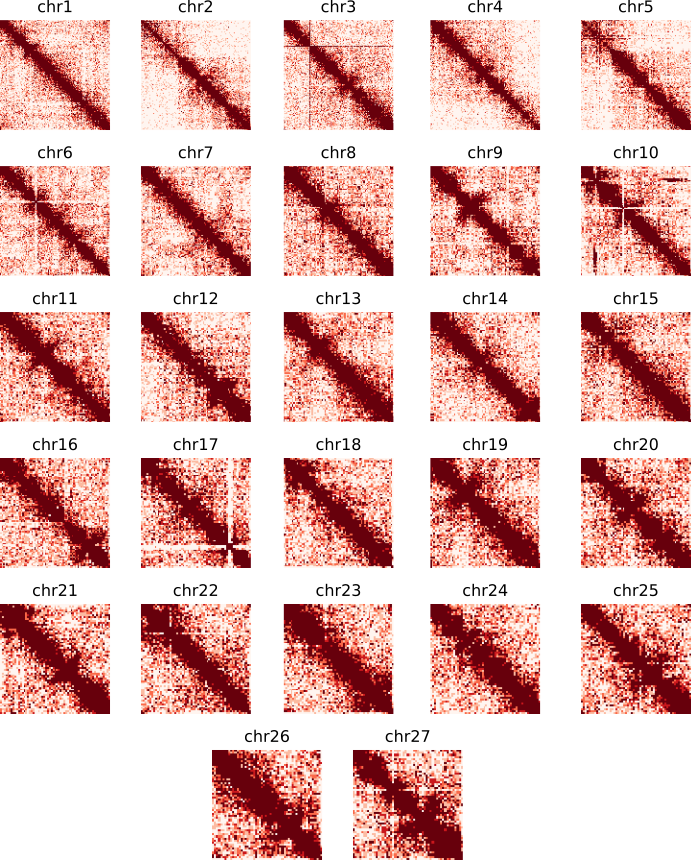
\includegraphics[width=13.5cm]{fig/instagraal/s11.png}
    \caption{All 27 newly formed scaffolds/putative chromosomes of \textit{Ectocarpus} sp. post-scaffolding at a 50-kb resolution. Centromere patterns are clearly apparent in all chromosomes, but some errors (potentially due to mapping issues) linger, such as chromosome 10 or 17.}
    \label{fig:instagraal_s11}
\end{figure}

\end{suppsection}

% write your paper in here

\chapter{Hi-C scaffolding of the bdelloid rotifer \textit{Adineta vaga}}

Bdelloid rotifers have been drawing interest due to their unusual ancient asexuality. A first diploid assembly of \textit{Adineta vaga} was published in 2013 \cite{flot2013}, with a total length of 218 Mb and a N50 of 260 kb, and the genome was described as "incompatible with conventional meiosis". In the following paper, the genome of \textit{Adineta vaga} was assembled \textit{de novo} using PacBio CLR, Nanopore reads, Illumina reads and Hi-C reads. Three assemblies were produced: a collapsed haploid assembly using all types of reads; and two diploid assemblies, one using PacBio CLR obtained with FALCON and FALCON-Unzip, and the second one using Illumina reads with Bwise. All these assemblies were scaffolded using instaGRAAL, and converged to 6 haploid chromosomes (collapsed assembly) or 12 phased chromosomes (FALCON-Unzip and Bwise assemblies). These results show that the genome of \textit{Adineta vaga} is: diploid, with 6 pairs of chromosomes; a paleotetraploid, as it has homoeologous chromosomes (pairs 1, 2 and 3 are homoeologous to pairs 4, 5, 6 respectively); and compatible with meiosis. \\
I contributed to this study in the assembly and Hi-C scaffolding of the collapsed haploid assembly. \\

%\begin{table}
%\caption{Comparison of assembly statistics with other genomes of the phylum Rotifera.}
%\resizebox{\columnwidth}{!}{
%\begin{tabular}{lllcccc}
%\hline
%\multirow{2}{*}{\textbf{Class}} & \multirow{2}{*}{\textbf{Species}} & \multirow{2}{*}{\textbf{Reads technology}} & %\textbf{Assembly} & \multirow{2}{*}{\textbf{N50}} & \multicolumn{2}{c}{\textbf{BUSCO}} \\
%    & & & \textbf{size} & & \textbf{single} & \textbf{dup.} \\
%\hline
%Bdelloida & \textit{Adineta vaga} & Illumina, Nanopore, PacBio, Hi-C & 101 Mb & 16.7 Mb &  &  \\
%    & \textit{Adineta vaga} \cite{flot2013} & Illumina, 454, mate pair & 218 Mb & 260 kb & 22.4\% & 64.8\% \\
%\hline
%Monogononta & \textit{Brachionus asplanchnoidis} \cite{brachionus_asplanchnoidis} & Illumina & 114 Mb & 10 kb & 82.O\% & 1.2\% \\
%    & \textit{Brachionus asplanchnoidis} \cite{brachionus_asplanchnoidis} & Illumina & 115 Mb & 9 kb &  &  \\
%\hline
%\end{tabular}
%}
%\label{tab:anthozoans}
%\end{table}

% write your paper in here

\chapter{Genome assembly of the coral \textit{Astrangia poculata}}

\section{Introduction}

The species \textit{Astrangia poculata} \cite{peters1988nomenclature}, also called the Northern star coral, is a temperate hard coral distributed across a wide range of latitudes in the western Atlantic ocean \cite{dimond2013simple}. It belongs to the class Anthozoa, a division of cnidarians that includes hard corals, soft corals, and sea anemones. Along with its adaptation to temperature variations, this coral has a facultative symbiosis with algae from the family Symbiodiniaceae, making it a compelling model to study coral response to environmental changes. To this end, we assembled its genome which will constitute a resource for downstream analysis. The genome had previously been assembled with a combination of Illumina and Hi-C reads; although this first version was highly contiguous, its size was excessively small compared to the expected genome size, and the draft had a poor completeness. I assembled the genome \textit{de novo} with newly sequenced Nanopore reads, which I combined with Illumina and Hi-C reads to produce an improved reference sequence. 

\section{Material \& Method}

\subsection{Sequencing data}

High-molecular-weight DNA was extracted by Dovetails Genomics. The sample was further purified with AMPure XP beads and fragments were selected on their size with Circulomics Short Reads Eliminator XS. \\
A Nanopore library was prepared with the Ligation Sequencing Kit LSK109, starting with 2.1 {\textmu}g of DNA, and yielded 1.4 {\textmu}g of DNA. The library was sequenced with a MinION on a R9.4 flowcell, with fast Guppy v4 basecalling. The flowcell was washed and reloaded three times (281 ng of DNA for the first load, 187 ng for subsequent loads) and ran for 89 hours. A total output of 6.79 Gb was obtained with an N50 of 18 kb and an N90 of 5 kb (Table \ref{tab:apoculata_datasets}). Adaptors were removed using Porechop \cite{porechop} with default parameters. After trimming, the dataset reached 6.77 Gb. \\

Dovetails Genomics produced two shotgun Illumina datasets of paired-end 150 bp reads: one with 414 million reads and an estimated insert size of 395 bp, and the second with 235 million reads and an estimated insert size of 484 bp (Table \ref{tab:apoculata_datasets}). Adaptors were removed using  cutadapt \href{https://github.com/marcelm/cutadapt}{github.com/marcelm/cutadapt}. \\

Dovetails Genomics also provided three Hi-C libraries with 198 million, 266 million and 257 million paired-end 150 bp reads (Table \ref{tab:apoculata_datasets}). The reads were trimmed of the adaptors with cutadapt.\\

\begin{table}[H]
\centering
\caption{\textit{Astrangia poculata} sequencing datasets.}
\begin{tabular}{|l|l|l|l|}
\hline
\textbf{Reads} & \textbf{Length} & \textbf{N50} & \textbf{Size} \\
\hline
Hi-C & 2*150 bp & - & 217 Gb \\
Illumina & 2*150 bp & - & 195 Gb\\
Nanopore & - & 18 kb & 7 Gb \\
\hline
\end{tabular}
\label{tab:apoculata_datasets}
\end{table}

\subsection{Genome size estimation}

Dovetails Genomics estimated the genome size to 462 Mb. I estimated the genome size using the second shotgun Illumina dataset of 235 million reads and the module kmercount.sh from BBtools \cite{bbtools}; the tool predicted a haploid size of 453 Mb, a ploidy of 2, and 40.95\% of repeats. 

\subsection{Genome assembly}

Five assemblers were tested with default parameters: Canu \cite{canu}, Ra \cite{ra}, Raven \cite{raven}, Flye \cite{flye}, wtdbg2 \cite{wtdbg2}. Purge Haplotigs \cite{purge_haplotigs} was run on the wtdbg2 assembly with default parameters, using the full shotgun Illumina datasets mapped with bowtie2 \cite{bowtie2}. The wtdbg2 assembly was polished with HyPo \cite{hypo}, using the full shotgun Illumina datasets mapped with bowtie2. Hi-C reads were mapped to the wtdbg2 assembly and processed using hicstuff \cite{hicstuff}, available at \href{https://github.com/koszullab/hicstuff}{github.com/koszullab/hicstuff}, with the parameters -{}-enzyme DpnII -{}-iterative -{}-aligner bowtie2. The draft assembly was then scaffolded using instaGRAAL \cite{instagraal}, with default parameters (-{}-levels 4 -{}-cycles 100 -{}-coverage-std 1, -{}-neighborhood 5). The output was refined with the module instaGRAAL-polish. \\

\subsection{Assembly evaluation}

BUSCO v4 \cite{busco_evaluation} was run against metazoa odb10 (954 features) without the parameter -{}-long. \textit{k}-mer completeness was calculated by running KAT comp v2.4.2 \cite{kat_evaluation} with the full shotgun Illumina datasets. The contact map was built using the hicstuff pipeline, with the three Hi-C libraries, and hicstuff view with the parameter \texttt{-{}-binning 200}. \\

\section{Results}

The assembly provided by Dovetails Genomics had chromosome-level scaffolds, but one of its major flaws was that its total size only reached 252 Mb (Table \ref{tab:apoculata_assembly_stats}) whereas the genome size was estimated to 462 Mb by Dovetails Genomics and to 453 Mb by BBtools. \\

\begin{table}[H]
\caption{Basic statistics of \textit{Astrangia poculata} assemblies, presenting the strategies that were used for each assembly (purging haplotigs, assembly polishing, scaffolding), assembly size, number of contigs, N50, number of BUSCO single complete features and BUSCO duplicate complete features.}
\resizebox{\columnwidth}{!}{
\begin{tabular}{lcccccccc}
\hline
\multirow{2}{*}{\textbf{Assembler}} & \multirow{2}{*}{\textbf{Purging}} & \multirow{2}{*}{\textbf{Polishing}} & \multirow{2}{*}{\textbf{Scaffolding}} & \multirow{2}{*}{\textbf{Assembly}} & \multirow{2}{*}{\textbf{\# contigs}} & \multirow{2}{*}{\textbf{N50}} & \multicolumn{2}{c}{\textbf{BUSCO}} \\
    &  &  &  & \textbf{size} &  &  & \textbf{single} & \textbf{dup.} \\
\hline
Dovetails & - & - & - & 252 Mb & 7848 & 16.8 Mb & 60.0\% & 0.2\% \\
\hline
Canu & $\times$ & $\times$ & $\times$ & 597 Mb & 8317 & 97 kb & 56.0\% & 7.9\% \\
\hline
Flye & $\times$ & $\times$ & $\times$ & 719 Mb & 7259 & 167 kb & 67.9\% & 8.9\% \\
\hline
Ra & $\times$ & $\times$ & $\times$ & 271 Mb & 2851 & 115 kb & 43.9\% & 0.3\% \\
\hline
Raven & $\times$ & $\times$ & $\times$ & 400 Mb & 2912 & 172 kb & 52.3\% & 0.4\% \\
\hline
wtdbg2 & $\times$ & $\times$ & $\times$ & 476 Mb & 4423 & 439 kb & 55.1\% & 0.3\% \\
    & \checkmark & $\times$ & $\times$ & 452 Mb & 2995 & 475 kb & 54.6\% & 0.3\% \\
    & \checkmark & \checkmark & $\times$ & 458 Mb & 2995 & 480 kb & 87.7\% & 2.4\% \\
    & \checkmark & \checkmark & \checkmark & 458 Mb & 488 & 31.0 Mb & 89.1\% & 1.2\% \\
\hline
\end{tabular}
}
\label{tab:apoculata_assembly_stats}
\end{table}

Ra and Raven both produced smaller assemblies than expected, with the Ra assembly size close to the one of Dovetails Genomics. Canu and Flye both produced assemblies quite larger than expected, which is likely due to uncollapsed haplotypes, as is shown by the increased percentages of duplicated BUSCO complete features. wtdbg2 produced the most convincing draft, with an assembly size close to expectations and the highest N50. Purge Haplotigs reduced the number of contigs from 4423 to 2995 and slightly increased the N50 from 439 kb to 475 kb. After polishing, the overall number of complete BUSCOs went from 54.9\% to 90.1\%. Scaffolding with instaGRAAL yielded 14 chromosome-level scaffolds, with sizes ranging from 21.1 Mb to 54.8 Mb. The final assembly contains 14 scaffolds and, after removing small sequences, has a size of 455 Mb and a BUSCO completeness of 90.4\%. The KAT plot shows two peaks, as the species is diploid \ref{fig:coral_kat}. Low multiplicity (or erroneous) \textit{k}-mers are absent from the assembly, as expected. A part of heterozygous \textit{k}-mers are represented once in the assembly and the rest are not, as only one haplotype is represented for heterozygous regions in collapsed haploid assemblies. The majority of homozygous \textit{k}-mers are represented once, although there are some missing and duplicated \textit{k}-mers. \\

\begin{figure}[H]
    \centering
    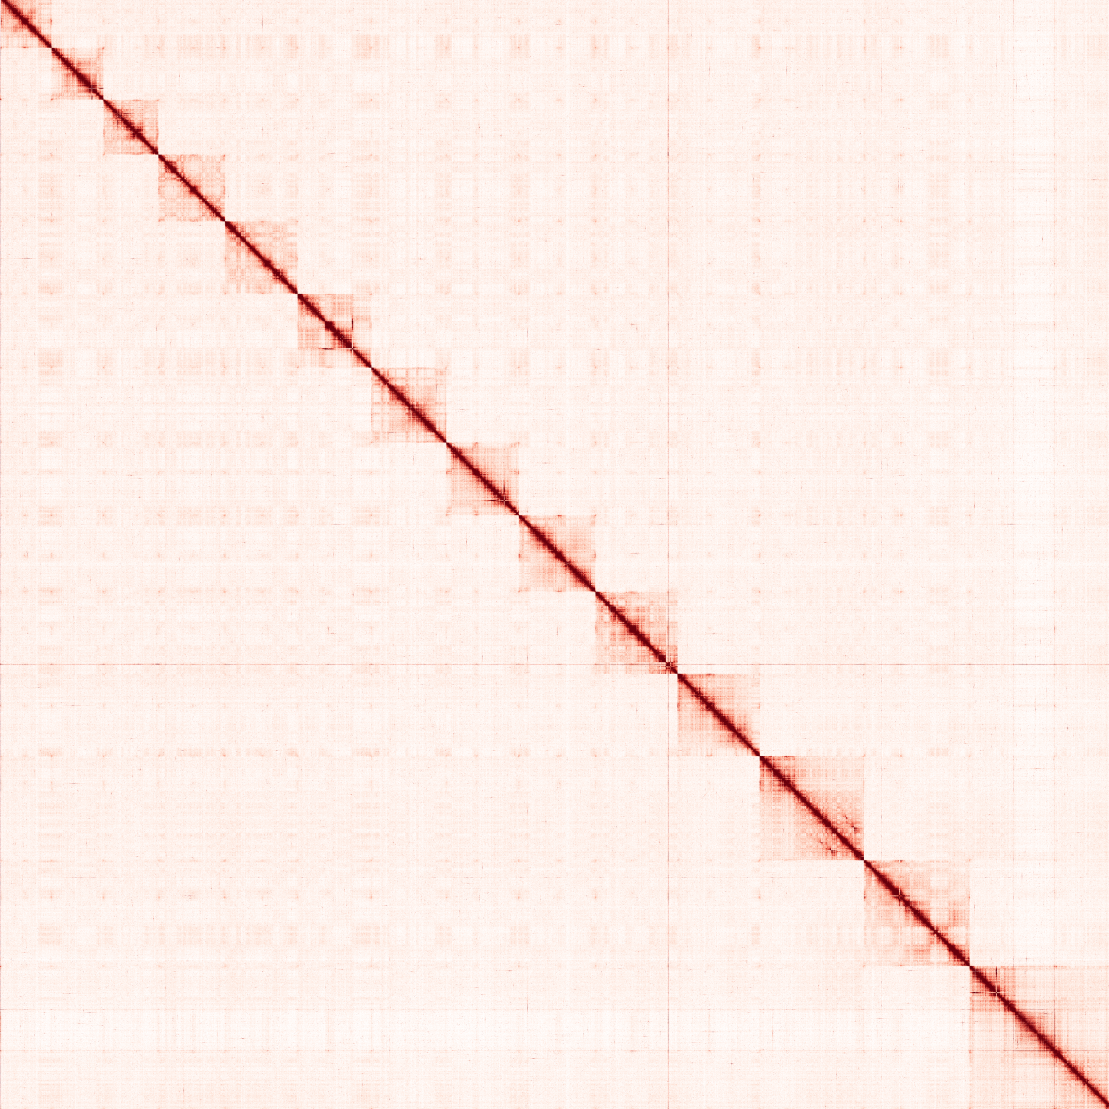
\includegraphics[width=0.9\linewidth]{fig/apoculata_contact_map_bin200.png}
    \caption{Contact map representing the 14 chromosome-level scaffolds of the final assembly (combining wtdbg2, Purge Haplotigs, HyPo and instaGRAAL).}
    \label{fig:coral_contact_map}
\end{figure}

\begin{figure}[H]
    \centering
    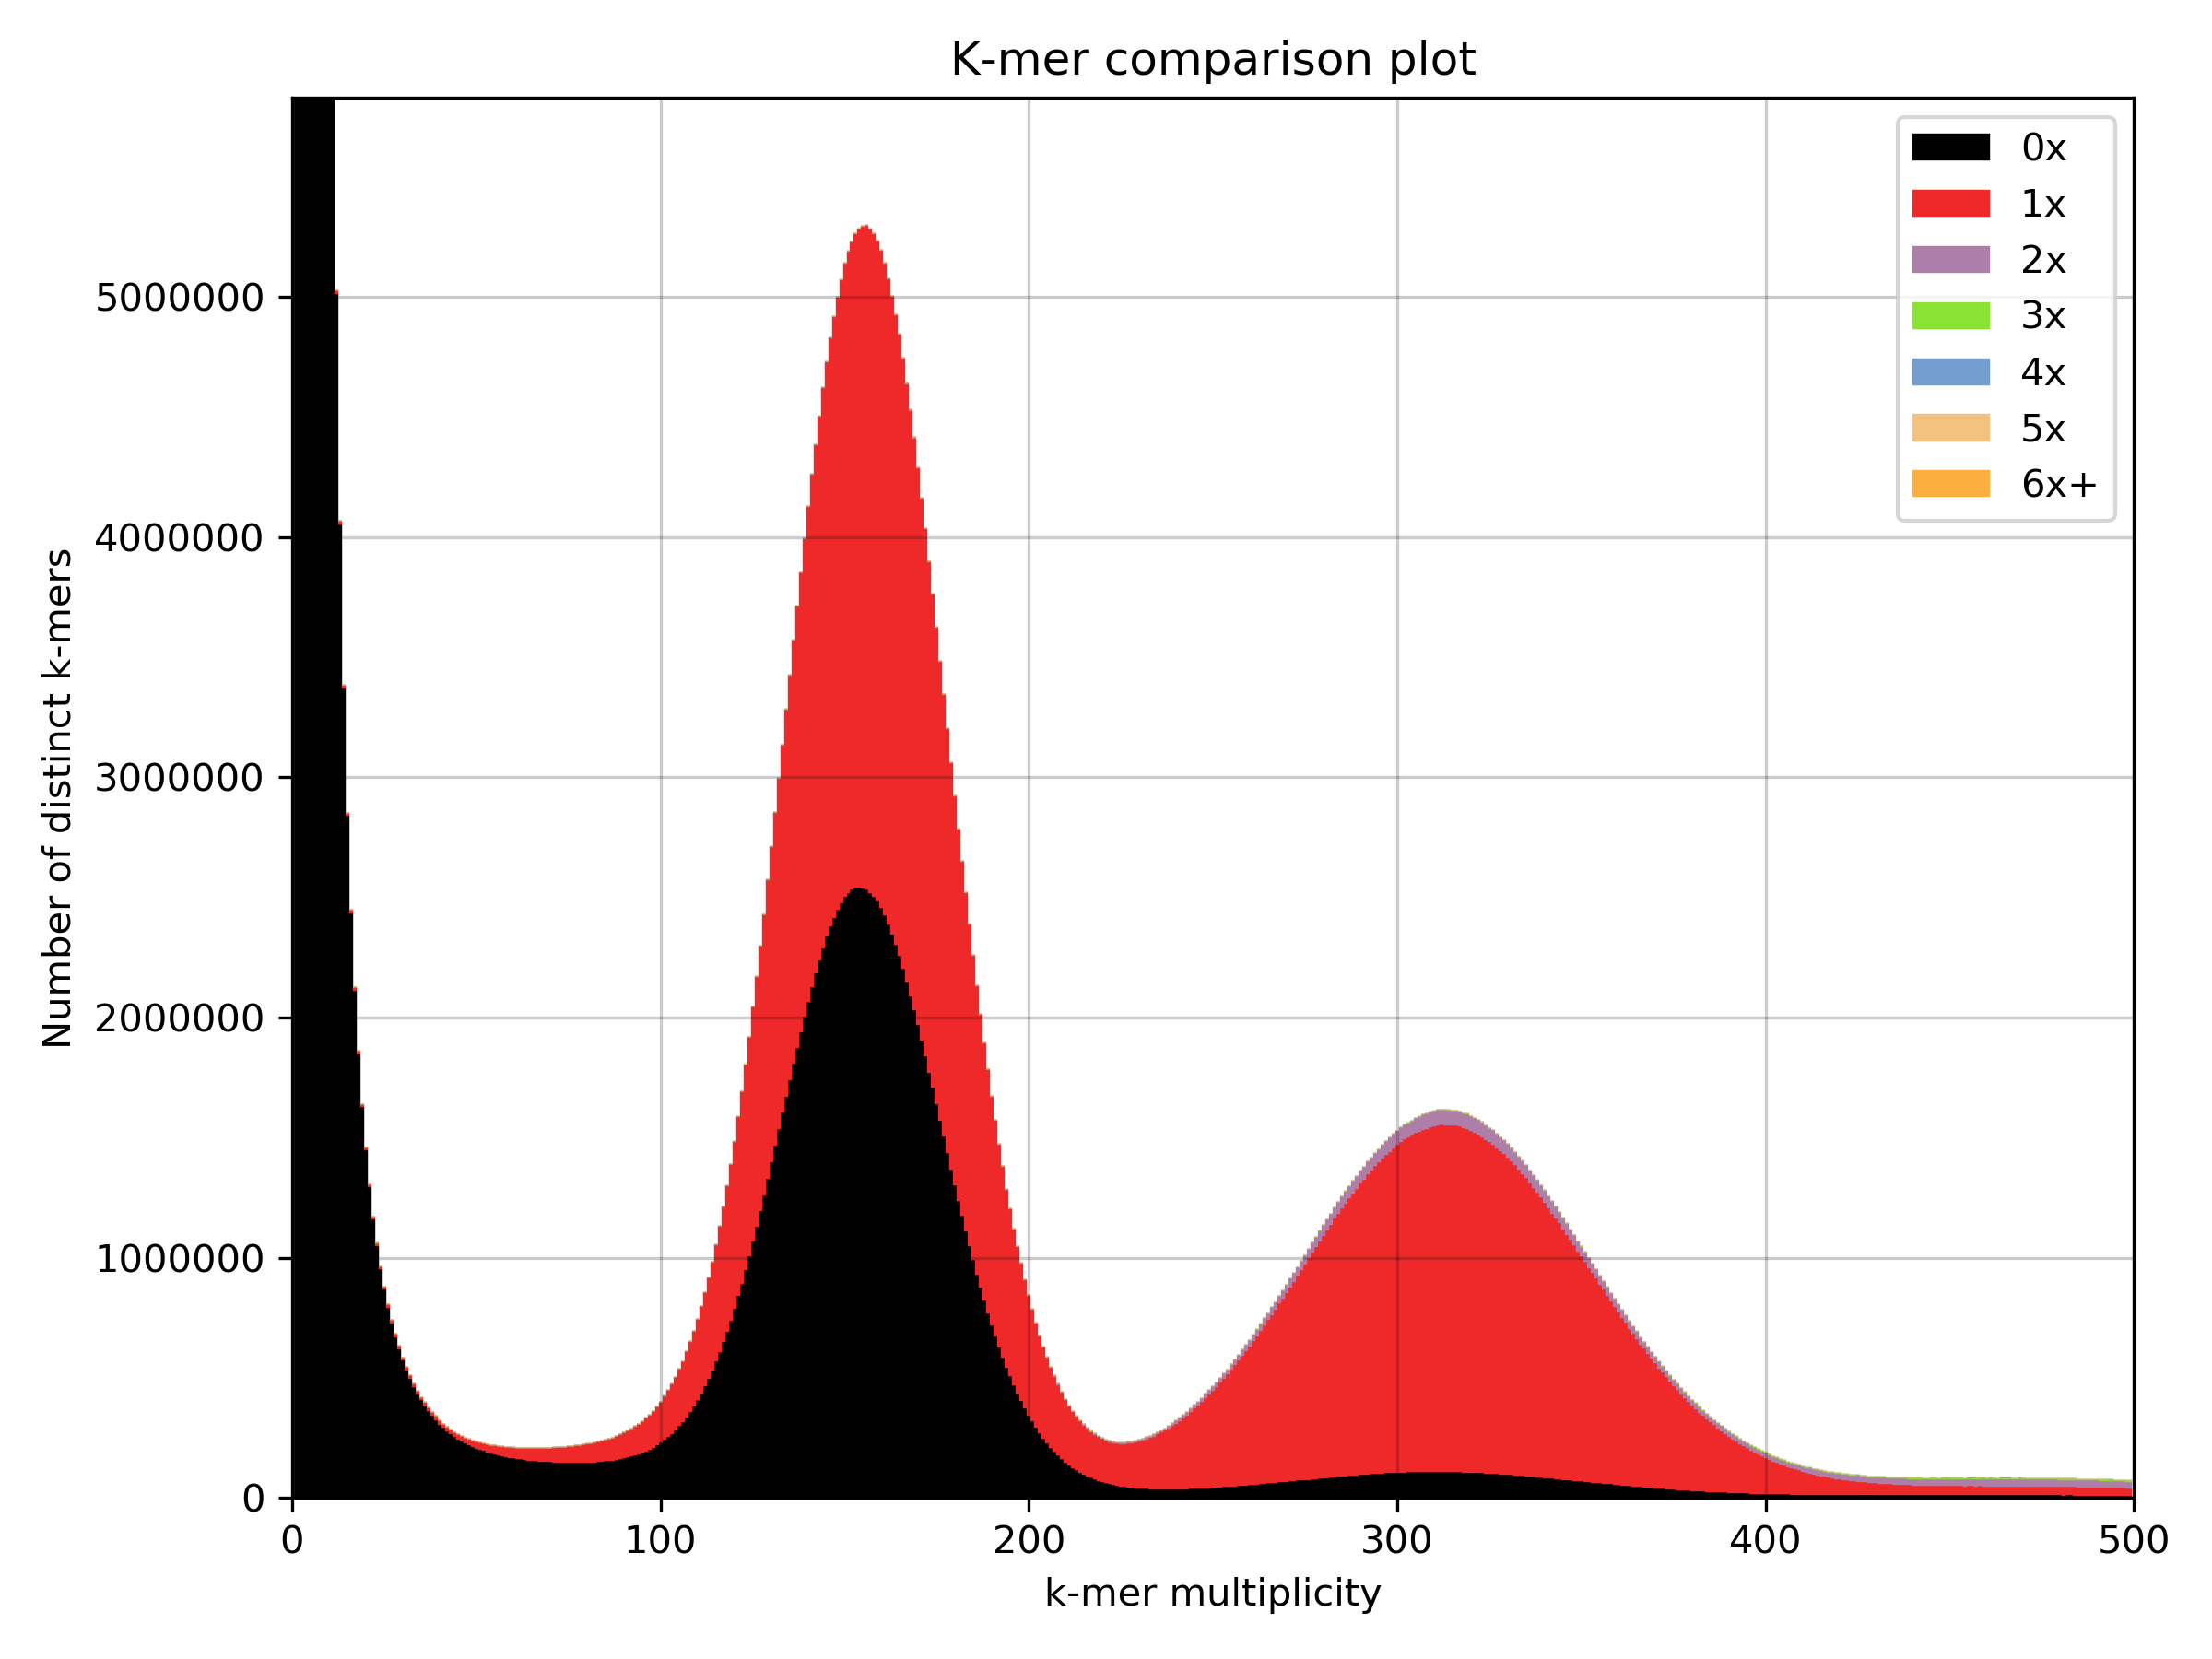
\includegraphics[width=0.9\linewidth]{fig/coral_kat.png}
    \caption{\textit{k}-mer analysis of the chromosome-level scaffolds of \textit{Astrangia poculata}. }
    \label{fig:coral_kat}
\end{figure}

\section{Discussion}

The initial assembly of \textit{Astrangia poculata} reached a high contiguity, but its small size and completeness indicated that the assembly was incomplete. The new assembly has a size and a number of chromosome-level scaffolds within the expected range, as well as high BUSCO and \textit{k}-mer completeness. This demonstrates that, although Hi-C scaffolding is a robust method to achieve chromosome-level assemblies, the quality of the input contigs is crucial. In this case, the small size of the initial assembly may result from the high repetitive content (estimated to 40.95\%) which is typically poorly handled by short reads; repeats are better resolved by long reads as their length can cover full repetitive regions \cite{pollard2018}. Interestingly, a low coverage of long reads (about 15X) was sufficient to yield an assembly with a size close to the estimated genome size, and polishing with a high-coverage short read dataset further improved the completeness. \\

Among assemblies of anthozoan genomes, only a few reached chromosome-level scaffolds: \textit{Acropora millepora}, \textit{Xenia} sp., and the assembly of \textit{Astrangia poculata} presented here (Table \ref{tab:anthozoans}). The most recent version of \textit{Acropora millepora} combines long reads, linked reads and genetic maps, while \textit{Xenia} sp. and \textit{Astrangia poculata} were both obtained with long reads, short reads, and Hi-C. One genome was scaffolded with an alternative \textit{in vitro} Hi-C protocol, called CHICAGO, but this approach led to a poor contiguity, and regular Hi-C should be favored for chromosome-level assemblies. Many genomes of hard corals (Scleractinia) were assembled with Illumina reads and scaffolded with mate pairs, and particularly for a large genomic analysis of their adaptation to elevated temperatures \cite{acropora_digitifera2}. All these assemblies have a size around 400 Mb, an overall BUSCO completeness over 88\% with few duplicated BUSCO features, and several have an N50 over 1 Mb. These assemblies, although obtained with short reads only, do not have the same flaws as the initial assembly of \textit{Astrangia poculata}, suggesting that short reads are still relevant to yield high-quality draft assemblies when combined with efficient assemblers (Platanus, in this case). Besides, the contiguity and completeness of the short-read only assemblies are comparable or higher compared to assemblies that included long reads. Hi-C scaffolding could be highly beneficial for the study of these genomes, as species of the genus Acropora have an endosymbiosis with zooxanthellae and Hi-C scaffolding can tell apart these different genomes. \\

The quality of the assembly of \textit{Astrangia poculata} makes it a new reliable reference among anthozoan genomes for downstrean analysis and comparison with other species. \\

%However, the high-molecular-weight DNA extraction and Hi-C library preparations were performed by a private company, thus no protocols are available which could have been used as a resource for other coral genome projects.

\begin{table}
\caption{Comparison of assembly statistics with other genomes of the class Anthozoa.}
\resizebox{\columnwidth}{!}{
\begin{tabular}{llllcccc}
\hline
\multirow{2}{*}{\textbf{Subclass}} &\multirow{2}{*}{\textbf{Order}} & \multirow{2}{*}{\textbf{Species}} & \multirow{2}{*}{\textbf{Reads technology}} & \textbf{Assembly} & \multirow{2}{*}{\textbf{N50}} & \multicolumn{2}{c}{\textbf{BUSCO}} \\
    & & & & \textbf{size} & & \textbf{single} & \textbf{dup.} \\
\hline
Hexacorallia & Scleractinia & \textit{Astrangia poculata} & Illumina, Nanopore, Hi-C & 455 Mb & 31 Mb & 89.2\% & 1.2\% \\
    & & \textit{Acropora acuminata} \cite{acropora_digitifera2} & Illumina, mate pair & 395 Mb & 1.0 Mb & 93.3\% & 0.7\% \\
    & & \textit{Acropora awi} \cite{acropora_digitifera2} & Illumina, mate pair & 429 Mb & 1.1 Mb & 89.0\% & 0.3\% \\
    & & \textit{Acropora cytherea} \cite{acropora_digitifera2} & Illumina, mate pair & 426 Mb & 1.1 Mb & 88.6\% & 2.9\% \\
    & & \textit{Acropora digitifera} \cite{acropora_digitifera1} & 454, Illumina, mate pair & 447 Mb & 484 kb & 67.7\% & 5.0\% \\
    & & \textit{Acropora digitifera} \cite{acropora_digitifera2} & Illumina, PacBio & 416 Mb & 1.9 Mb & 91.6\% & 0.6\% \\
    & & \textit{Acropora echinata} \cite{acropora_digitifera2} & Illumina, mate pair & 401 Mb & 1.9 Mb & 88.2\% & 0.3\% \\
    & & \textit{Acropora florida} \cite{acropora_digitifera2} & Illumina, mate pair & 443 Mb & 751 kb & 89.1\% & 1.7\% \\
    & & \textit{Acropora gemmifera} \cite{acropora_digitifera2} & Illumina, mate pair & 401 Mb & 1.1 Mb & 87.3\% & 0.7\% \\
    & & \textit{Acropora hyacinthus} \cite{acropora_digitifera2} & Illumina, mate pair & 447 Mb & 1.6 Mb & 91.4\% & 1.6\% \\
    & & \textit{Acropora intermedia} \cite{acropora_digitifera2} & Illumina, mate pair & 417 Mb & 577 kb & 90.6\% & 1.8\% \\
    & & \textit{Acropora microphthalma} \cite{acropora_digitifera2} & Illumina, mate pair & 384 Mb & 1.1 Mb & 88.6\% & 1.4\% \\
    & & \textit{Acropora millepora} \cite{acropora_millepora1} & Illumina, mate pair & 387 Mb & 495 kb & 92.3\% & 0.7\% \\
    & & \textit{Acropora millepora \cite{hic_genomes}} & Illumina, mate pair, Hi-C & 387 Mb & 22.6 Mb & 91.7\% & 0.7\% \\
    & & \textit{Acropora millepora} \cite{acropora_millepora2} & PacBio, linked reads, genetic map & 475 Mb & 19.8 Mb & 91.9\% & 1.5\% \\
    & & \textit{Acropora muricata} \cite{acropora_digitifera2} & Illumina, mate pair & 421 Mb & 575 kb & 87.4\% & 1.7\% \\
    & & \textit{Acropora nasuta} \cite{acropora_digitifera2} & Illumina, mate pair & 416 Mb & 1.1 Mb & 89.4\% & 2.5\% \\
    & & \textit{Acropora selago} \cite{acropora_digitifera2} & Illumina, mate pair & 393 Mb & 657 kb & 87.8\% & 1.3\% \\
    & & \textit{Acropora tenuis} \cite{acropora_digitifera2} & Illumina, mate pair & 403 Mb & 1.2 Mb & 91.6\% & 0.8\% \\
    & & \textit{Acropora yongei} \cite{acropora_digitifera2} & Illumina, mate pair & 438 Mb & 3.0 Mb & 89.9\% & 1.2\% \\\
    & & \textit{Montipora cactus} \cite{acropora_digitifera2} & Illumina, mate pair & 653 Mb & 899 kb & 89.4\% & 0.9\% \\
    & & \textit{Montipora capitata} \cite{montipora_capitata1} & PacBio & 886 Mb & 541 kb & 75.7\% & 16.9\% \\
    & & \textit{Montipora capitata} \cite{montipora_capitata2} & Linked reads & 615 Mb & 186 kb & 79.7\% & 0.5\% \\
    & & \textit{Montipora efflorescens} \cite{acropora_digitifera2} & Illumina, mate pair & 643 Mb & 1.1 Mb & 88.4\% & 0.9\% \\
    & & \textit{Orbicella faveolata} \cite{orbicella_faveolata} & Illumina, mate pair & 486 Mb & 1.6 Mb & 82.7\% & 2.3\% \\
    & & \textit{Pocillopora damicornis} \cite{pocillopora_damicornis} & Illumina, CHICAGO & 234 Mb & 326 kb & 88.5\% & 0.4\% \\
    & & \textit{Stylophora pistillata} \cite{stylophora_pistillata} & Illumina, mate pair & 400 Mb & 457 kb & 87.6\% & 0.5\% \\
    & Actiniaria & \textit{Actinia equina} \cite{actinia_equina} & PacBio & 409 Mb & 493 kb & 65.1\% & 29.5\% \\
    & & \textit{Actinia tenebrosa} \cite{actinia_tenebrosa} & Illumina, mate pair & 238 Mb & 189 kb & 91.4\% & 0.6\% \\
    & & \textit{Exaiptasia pallida} \cite{exaiptasia_pallida} & Illumina, mate pair & 256 Mb & 442 kb & 84.0\% & 2.6\% \\
    & & \textit{Nematostella vectensis} \cite{nematostella_vectensis} & Sanger & 357 Mb & 473 kb & 91.7\% & 1.8\% \\
    & Corallimorpharia & \textit{Amplexidiscus fenestrafer} \cite{amplexidiscus_fenestrafer} & Illumina, mate pair & 370 Mb & 510 kb & 84.4\% & 0.5\% \\
    & & \textit{Discosoma} sp. \cite{amplexidiscus_fenestrafer} & Illumina, mate pair & 444 Mb & 772 kb & 85.2\% & 2.1\% \\
\hline
Octocorallia & Alcyonacea & \textit{Dendronephtya gigantea} \cite{dendronephthya_gigantea} & Illumina, PacBio & 286 Mb & 1.4 Mb & 84.3\% & 8.3\% \\
    & & \textit{Paramuricea clavata} \cite{paramuricea_clavata} & Illumina, Nanopore & 607 Mb & 24 kb & 72.5\% & 1.3\% \\
    & & \textit{Xenia} sp. \cite{xenia_sp} & Illumina, Nanopore, Hi-C & 223 Mb & 14.8 Mb & 85.1\% & 2.1\% \\
    & Pennatulacea & \textit{Renilla muelleri} \cite{renilla_muelleri} & Illumina, PacBio & 172 Mb & 71 kb & 85.2\% & 3.1\% \\
\hline
\end{tabular}
}
\label{tab:anthozoans}
\end{table}

% write your paper in here

\chapter{Genome assembly of the chaetognath \textit{Flaccisagitta enflata}}

\section{Introduction}

Chaetognaths, commonly known as arrow worms, are transparent marine predators widely distributed all over the oceans and at various depths, although most species are found at low depth \cite{alvarino1964bathymetric}. They are characterized by a transparent and elongated body, with one or two pairs of lateral fins, and one caudal fin, a head with hooks and a size ranging from a few millimeters to several centimeters \cite{ghirardelli1969}. Current chaetognath species are divided into two orders depending on the presence of transversal muscles, or phragms: Phragmophora and Aphragmophora. The whole phylum now encompasses about 150 species. They form an enigmatic clade whose phylogenetic position is still being discussed. Chaetognaths were initially considered as deuterostomians, due to their development, but analyses of 18S rDNA rejected this hypothesis \cite{telford1993phylogenetic,wada1994details} and further brought support to the Phragmophora and Aphragmophora branches \cite{telford1997evolution}. Later, Nielsen suggested that chaetognaths belonged to the clade Gnathifera \cite{nielsen2011}, which gathers Gnathostomulida, Micrognathozoa and Rotifera. This hypothesis was supported by a recent transcriptome analysis of ten chaetognath species \cite{marletaz2019new}.  \\
To this day, there is no genome assembly available for the whole phylum Chaetognatha, although this resource could resolve their phylogenetic position. I assembled the genome of the species \textit{Flaccisagitta enflata}, which was first described by Grassi in 1881; it belongs to the order Aphragmophora and the family Sagittidae. It is epipelagic and present across all oceans in warmer waters \cite{michel1984}. This species was selected based on specimen sizes (up to 2.5 cm), to avoid pooling individuals for sequencing, and its moderate genome size, estimated to 0.71 picograms (pg) \cite{animal_genome_size}. \\

\section{Material \& Method}

\subsection{Collection and fixation}

Chaetognaths were collected around the island of Curaçao after sunset from October 29th to November 2nd 2019. A total of 30 individuals were sampled: 11 were crosslinked in 3\% formaldehyde for 30 to 45 minutes, quenched in 250 mM glycine, then frozen at -80{\degree}C; 12 were preserved in absolute ethanol and kept at 4{\degree}C; 7 were preserved in RNAlater and kept at 4{\degree}C. All samples used for DNA, RNA and Hi-C sequencing were collected on November 2nd 2019 in Snake Bay.

\subsection{High-molecular-weight DNA extraction}

One 2-cm individual preserved in ethanol was incubated in 180 {\textmu}L of CTAB buffer (described in Table \ref{tab:ctab}) and 25 µL of proteinase K for 3 hours at 60{\degree}C and 300 rpm. The lysed sample was purified with phenol-chloroform-isoamyl alcohol 25:24:1, chloroform-isoamyl alcohol 24:1 and with AMPure XP beads. I obtained 2.5 µg of DNA with OD260/280 = 1.95 and OD260/230 = 1.95.

\begin{table}[H]
\centering
\begin{tabular}{|l|l|l|}
\hline
\textbf{Solution} & \textbf{Stock concentration} & \textbf{Volume for 2.45 mL} \\
\hline
PVP & 10\% & 500 {\textmu}L \\
Tris-HCl & 1 M & 250 {\textmu}L \\
EDTA & 500 mM & 125 {\textmu}L \\
NaCl & 5 M & 1 mL \\
H\textsubscript{2}O & - & 75 {\textmu}L \\
CTAB & 10\% & 500 {\textmu}L \\
{\textbeta}-mercaptoethanol & - & 25 {\textmu}L \\
\hline
\end{tabular}
\caption{Composition of CTAB buffer.}
\label{tab:ctab}
\end{table}

\subsection{Whole-genome sequencing}

The library for Nanopore sequencing was prepared with the Nanopore SQK-LSK109 Ligation sequencing kit. This library was loaded four times in the PromethION flow cell with nuclease flushes in between. The flow cell (with pore proteins R9.4.1) ran for 72 hours and gave an output of 40.5 Gb with an N50 = 6.1 kb. Basecalling was done with Guppy v4. 168 Gb of paired-end 150-bp Illumina reads were also sequenced by Novogene.

%\begin{figure}[H]
%    \centering
%    \includegraphics[width=0.9\linewidth]{fig/fenflata_ONT_read_length_distribution.png}
%    \caption{Read length distribution of Nanopore reads up to 50 kb (bin = 500 bases).}
%    \label{fig:histo_ONT}
%\end{figure}

%\subsection{RNA extraction and sequencing}

%One 1.2-cm individual preserved in RNAlater was mixed in 1 mL Trizol. Then the sample was purified with 200 {\textmu}L of chloroform-isoamyl alcohol, and the RNA was recovered using 500 {\textmu}L of isopropanol. With this protocol, I obtained 3.4 {\textmu}g of RNA with OD260/280 = 1.79 and OD260/230 = 1.95. The cDNA sequencing library was prepared using the Nanopore PCR-cDNA sequencing kit and was sequenced using a MinION flow cell, which yielded 909 Mb and 1.98 million reads. RNA was also extracted from another 1.8-cm individual preserved in RNAlater by Novogene, using a similar Trizol-based protocol. This sample was sequenced on a NovaSeq platform and yielded 201 millions pairs of reads of 150 bases. 

\subsection{Hi-C sequencing}

One 1.5-cm individual crosslinked in 3\% formaldehyde was used to prepare a Hi-C library with the Arima Hi-C kit (including the restriction enzymes DpnII and HinfI), and resulted in 466 ng of DNA. The DNA was fragmented with a Covaris (300 bp) and biotinylated fragments were selected with streptavidin beads. The library was prepared for Illumina sequencing using Invitrogen TM Collibri TM PS DNA Library Prep Kit and following manufacturer instructions. Sequencing by Novogene resulted in 489 millions pairs of reads of 150 bp.

\subsection{Pre-assembly analysis}

The genome size was estimated with BBtools \cite{bbtools} using the script \texttt{kmercountexact.sh} and the shotgun Illumina reads. As this tool is based on \textit{k}-mers, three values of \textit{k} were tested with \textit{k} = \{27, 29, 31\}. A \textit{k}-mer histogram of the Illumina dataset was built using KAT hist v2.4.2 (with \textit{k} = 27). 

\subsection{Genome assembly}

The Nanopore reads were trimmed using Porechop \cite{porechop} with default parameters, then they were assembled \textit{de novo} with several assemblers: Canu \cite{canu}, Flye \cite{flye}, Ra \cite{ra}, Raven \cite{raven} and wtdbg2 \cite{wtdbg2}. The assemblies were polished with HyPo \cite{hypo} and remaining uncollapsed haplotypes were purged with purge\_dups \cite{purge_dups} and Purge Haplotigs \cite{purge_haplotigs}. I also tried preprocessing the reads by filtering them using a length threshold or the tool Filtlong with the parameters \texttt{-{}-keep\_percent 52.0 -{}-min\_length 2000}. Assembly pipelines were defined following the strategies identified in Chapter 2. Two assemblies were selected as candidates for Hi-C scaffolding:
\begin{itemize}
    \item[--] FEv1: Ratatosk + Canu + purge\_dups x2
    \item[--] FEv2: Raven + HyPo + purge\_dups + Purge Haplotigs
\end{itemize}

\subsection{Hi-C scaffolding}

Hi-C reads were mapped to the draft assemblies using hicstuff \cite{hicstuff} with the parameters \texttt{-{}-enzyme DpnII,HinfI -{}-aligner bowtie2 -{}-iterative}. instaGRAAL was run with the parameters \texttt{-{}-level 5 -{}-cycles 150}. The scaffolds were post-processed with instaGRAAL-polish to reduce misassemblies and 10 Ns were added as gaps.

\subsection{Gap filling}

Gaps in the scaffolded assemblies were filled by TGS-GapCloser \cite{tgsgapcloser} using the Ratatosk-corrected Nanopore reads for FEv1 and the Nanopore reads for FEv2. FEv1 was further polished using HyPo. 

\subsection{Assembly evaluation}

Assemblies were assessed using BUSCO v4 against the lineage metazoa odb10 without the parameter \texttt{-{}-long} and using KAT comp 2.4.2 against the Illumina dataset (with \textit{k} = 27. Contact maps were built for scaffolded assemblies using the hicstuff pipeline as described previously and hicstuff view with the parameter \texttt{-{}-binning 2000}.

\section{Results}

\subsection{Species identification}

Morphological characteristics were registered in living and fixed individuals in order to identify the species: 
\begin{itemize}
    \item[--] longest specimen of 2.5 cm;
    \item[--] the body is transparent, soft and looks enflated;
    \item[--] 8-10 hooks (Figure 1.A1);
    \item[--] absence of collarette;
    \item[--] anterior position of the ganglion (Figure 1.A2);
    \item[--] pair of lateral fins;
    \item[--] short rounded fins;
    \item[--] ovaries do not extend to the anterior fins (Figure 1.B3);
    \item[--] round vesicles close to the tail (Figure 1.B4).
\end{itemize}

\begin{figure}[H]
    \centering
    \includegraphics[width=0.9\linewidth]{fig/rect1951.png}
    \caption{A chaetognath specimen fixated in 3\% formaldehyde. This individual was used for Hi-C sequencing.}
\end{figure}

The specimens were all identified as \textit{Flaccisagitta enflata} using the identification key provided in Michel \cite{michel1984}. 

\subsection{Whole-genome assembly}

The haploid genome size was estimated to 695-699 Mb, which matches the value available on the Animal Genome Size Database \cite{animal_genome_size} of 0.71 picograms (approximately 694 Mb), measured with Feulgen densitometry. The \textit{k}-mer histogram shows two distinct peaks, one around 85X, for heterozygous \textit{k}-mers, and a second around 172X, for homozygous \textit{k}-mers, thus the genome is diploid (Figure \ref{fig:fenflata_kat_hist}). The homozygous peak is strikingly small compared to the heterozygous peak, indicating a high level of heterozygosity. 

\begin{figure}
    \centering
    \includegraphics[width=1\linewidth]{fig/fenflata_kat_illumina.eps}
    \caption{\textit{k}-mer analysis of the Illumina dataset.}
    \label{fig:fenflata_kat_hist}
\end{figure}

Most initial assemblies had a size larger than the expected genome size (Table \ref{tab:chaeto_assemblies}), due to the high heterozygosity of the genome that leads to artefactual duplications, as described in Chapter 2. Canu and Flye tend to retain uncollapsed haplotypes; Flye yielded an assembly about twice the expected haploid size when using all raw Nanopore reads (1.45 Gb), suggesting a diploid assembly, but surprisingly Canu produced a smaller assembly than expected (614 Mb). These behaviors were reversed with the Ratatosk-corrected Nanopore dataset: the Canu assembly was likely diploid (1.48 Gb), while the Flye assembly was close to the haploid genome size (849 Mb). However, the poor BUSCO score of the Ratatosk-Flye assembly suggested that it was not a good candidate. Two rounds of purge\_dups greatly improved the Canu-Ratatosk and Flye-HyPo assemblies, as the number of duplicated BUSCO features were reduced in favor of single-copy BUSCO features. The Ratatosk-Canu-purge\_dups assembly (designated as FEv1) was selected for scaffolding based on its high BUSCO score, low duplicated features and contiguity. The Ra assembly of raw Nanopore reads longer than 5 kb was the closest to the expected genome size (728 Mb), yet the BUSCO score after polishing is low (80.4\% single-copy and duplicated features). The Raven assembly of all raw reads was oversized, and after polishing the BUSCO score indicated a large amount of duplications (30.9\% duplicated features). A combination of purge\_dups and Purge Haplotigs diminished the number of duplicated features (11.6\%) and increased the single-copy BUSCO score (78.9\%); this assembly was selected for scaffolding as FEv2. The wtdbg2 assembly had a moderate amount of duplications, but its BUSCO completeness after polishing was still lower than FEv1 and FEv2.

\begin{table}
\centering
\caption{Assembly statistics. purge\_dups and Purge Haplotigs are respectively designated as PD and PH.}
\resizebox{\columnwidth}{!}{
\begin{tabular}{lccccccccccc}
   \hline
    \multirow{2}{*}{\textbf{Assembly}} & \textbf{Read} & \textbf{Hybrid} & \multirow{2}{*}{\textbf{Polishing}} & \textbf{Haplotig} & \textbf{Assembly} & \multirow{2}{*}{\textbf{\# contigs}} & \multirow{2}{*}{\textbf{N50}} & \textbf{Largest} & \multicolumn{2}{c}{\textbf{BUSCO}} \\
        & \textbf{selection} & \textbf{correction} &  & \textbf{purging} & \textbf{size} &  &  & \textbf{contig} & \textbf{single} & \textbf{dup.} \\
    \hline
    Canu & 5 kb & $\times$ & $\times$ & $\times$ & 614 Mb & 24038 & 44 kb & 497 kb & 27.6\% & 2.7\% \\
        & $\times$ & Ratatosk & $\times$ & $\times$ & 1.48 Gb & 13385 & 195 kb & 1.2 Mb & 28.3\% & 66.0\% \\
        & $\times$ & Ratatosk & $\times$ & PD x2 & 946 Mb & 9288 & 215 kb & 1.2 Mb & 85.4\% & 7.1\% \\
    \hline
    Flye & $\times$ & $\times$ & $\times$ & $\times$ & 1.45 Gb & 31205 & 264 kb & 1.6 Mb & 61.1\% & 12.3\% \\
        & $\times$ & Ratatosk & $\times$ & $\times$ & 849 Mb & 40273 & 50 kb & 967 kb & 43.9\% & 47.1\% \\
        & $\times$ & $\times$ & HyPo & $\times$ & 1.45 Gb & 31205 & 263 kb & 1.6 Mb & 35.0\% & 58.8\% \\
        & $\times$ & $\times$ & HyPo & PD x2 & 985 Mb & 9508 & 277 kb & 1.6 Mb & 71.2\% & 19.8\% \\
    \hline
    Ra & 5 kb & $\times$ & $\times$ & $\times$ & 728 Mb & 7706 & 110 kb & 509 kb & 42.9\% & 1.3\% \\
        & 5 kb & $\times$ & HyPo & $\times$ & 730 Mb & 7706 & 111 kb & 510 kb & 68.8\% & 11.6\% \\
        & Filtlong & $\times$ & $\times$ & $\times$ & 684 Mb & 7507 & 106 kb & 498 kb & 39.7\% & 0.6\% \\
    \hline
    Raven & $\times$ & $\times$ & $\times$ & $\times$ & 1.10 Gb & 7656 & 185 kb & 1.2 Mb & 60.0\% & 6.0\% \\
        & 5 kb & $\times$ & $\times$ & $\times$ & 1.01 Gb & 6901 & 180 kb & 864 kb & 37.8\% & 0.9\% \\
        & Filtlong & $\times$ & $\times$ & $\times$ & 1.01 Gb & 6741 & 186 kb & 1.0 Mb & 36.3\% & 1.3\% \\
        & $\times$ & $\times$ & HyPo & $\times$ & 1.10 Gb & 7656 & 186 kb & 1.2 Mb & 61.1\% & 30.9\% \\
        & $\times$ & $\times$ & HyPo & PD + PH & 929 Mb & 6612 & 191 kb & 1.2 Mb & 78.9\% & 11.6\% \\
    \hline
    wtdbg2 & $\times$ & $\times$ & $\times$ & $\times$ & 965 Mb & 13558 & 219 kb & 2.0 Mb & 19.3\% & 0.2\% \\
        & $\times$ & $\times$ & HyPo & $\times$ & 987 Mb & 13558 & 224 kb & 2.1 Mb & 71.5\% & 13.1\% \\
    \hline
\end{tabular}
}
\label{tab:chaeto_assemblies}
\end{table}

The mapping rate of Hi-C reads was low for both FEv1 and FEv2: only 37\% of the reads mapped uniquely. Scaffolding with instaGRAAL yielded 9 chromosome-level scaffolds (Table \ref{tab:chaeto_scaffolded_assemblies}, Figure \ref{fig:fenflata_contact_maps}), and only these scaffolds were retained for the final assemblies, to discard contamination from bacteria and plankton in the digestive tube. The cumulative sizes of the 9 scaffolds are close to the expected genome size yet still higher (794 Mb for FEv1, 745 Mb for FEv2). The scaffolds are notably larger in FEv1 than in FEv2, but the contact maps are similar. FEv1 has the lowest number of Ns in gaps, and its BUSCO score is higher as well. As for the \textit{k}-mer spectra (Figure \ref{fig:fenflata_kat_comp}), both FEv1 and FEv2 have some remaining duplicated \textit{k}-mers in the homozygous peak. Nevertheless, most homozygous \textit{k}-mers are represented once, part of heterozygous \textit{k}-mers are represented once, and the rest are not included in the assembly, as is expected for a collapsed assembly of a diploid genome. There is yet fewer missing homozygous \textit{k}-mers in FEv1 than in FEv2.

\begin{table}[H]
\centering
\caption{Comparison of scaffolded assemblies.}
\begin{tabular}{lcccccc}
   \hline
    \multirow{2}{*}{\textbf{Assembly}} & \textbf{Assembly} & \textbf{Chromosomes} & \multirow{2}{*}{\textbf{N count}} & \multicolumn{3}{c}{\textbf{BUSCO}} \\
        & \textbf{size} & \textbf{lengths} &  & \textbf{overall} & \textbf{single} & \textbf{dup.} \\
    \hline
    FEv1 & 794 Mb & 71-112 Mb & 23,555 & 93.3\% & 86.9\% & 6.4\% \\
    FEv2 & 745 Mb & 59-105 Mb & 84,572 & 87.6\% & 83.3\% & 4.3\% \\
    \hline
\end{tabular}
\label{tab:chaeto_scaffolded_assemblies}
\end{table}

\begin{figure}[H]
    \centering
    \includegraphics[width=1\linewidth]{fig/fenflata_contact_maps_scaffolded.png}
    \caption{Contact maps of chromosome-level scaffolds for the two Hi-C scaffolded assemblies.}
    \label{fig:fenflata_contact_maps}
\end{figure}

\begin{figure}[H]
    \centering
    \includegraphics[width=1\linewidth]{fig/fenflata_kat_scaffolded.eps}
    \caption{\textit{k}-mer analysis of chromosome-level scaffolds for the two Hi-C scaffolded assemblies.}
    \label{fig:fenflata_kat_comp}
\end{figure}

\section{Discussion}

The genome of \textit{Flaccisagitta enflata} posed a challenge on several aspects. The amount of DNA that could be extracted from one specimen was too low to run all analysis on a single individual, but it was however sufficient to avoid pooling individuals for long-read sequencing or for Hi-C sequencing. First analysis showed that it was even more desirable to assemble the contigs from only one individual as the genome has a high heterozygosity; thus, a pool of highly divergent individuals would have further hindered the assembly. Using a second individual for Hi-C sequencing is a likely cause for the low mapping rate, due to the variability from one specimen to another. Besides, the collapsed assembly only represents one haplotype for all heterozygous regions; as this genome has a high heterozygosity, many Hi-C reads may fail to map to the missing haplotypes. Considering the level of heterozygosity, a diploid assembly would have been a more complete representation. Such assembly is possible when combining short and long reads, as for the Ratatosk-Canu assembly, but phasing with Hi-C is impossible in this case as the datasets were generated from different specimens. \\
Despite these difficulties, the FEv1 and FEv2 assemblies reached high contiguity and completeness. The draft long-read assemblies had a relatively small N50, which may be to the numerous heterozygous regions causing unresolved bubbles in the assembly graphs and leading to breaks. Still, Hi-C scaffolding with instaGRAAL brought these assemblies to chromosome level; although no karyotype is available for this species, FEv1 and FEv2 both converged towards 9 chromosome-level scaffolds. \\
This study will serve as a basis for chaetognath genomics, since this is the first chaetognath assembly. Future phylogenomic analyses may shed light on the puzzling position of this clade, and bring insights into its evolution. In addition, the methods used for this project should facilitate new chaetognaths assemblies as it provides resources for high-molecular-weight DNA extraction, Nanopore sequencing, Hi-C sequencing, and assembly.

\chapter{Discussion \& Conclusion}

\section{Combining long reads and Hi-C for chromosome-level assemblies}

Long reads and Hi-C are undoubtedly a winning combination to obtain chromosome-level assemblies with high completeness. Long reads have disrupted the field of genome assembly and brought compelling new techniques in addition to short-read sequencing. Long-read sequencing is more laborious than short reads due to its requirement for high-molecular-weight DNA, yet long-read assemblies are generally favored for their higher contiguity and better resolution of repeats. However, long reads are often not sufficient to assemble eukaryote genomes into chromosome-level contigs. Increasing the sequencing depth may improve the contiguity to a certain extent, but long-read assemblers do not seem able to take advantage of huge sequencing depths (up to 230X of PacBio CLR and 170X of Nanopore reads in the case of \textit{Adineta vaga}) to fully solve assemblies. Scaffolding is still a necessary step, and Hi-C has emerged as the most robust method to bring assemblies to chromosome level. The popularity of Hi-C has stimulated the release of protocols, commercial kits and tools, providing researchers with a variety of options to adapt to their genome projects. The genomes presented here, \textit{Adineta vaga}, \textit{Astrangia poculata} and \textit{Flaccisagitta enflata}, were assembled with a mix of short reads, long reads and Hi-C, and all reached chromosome-level scaffolds with high completeness. The genome assembly of \textit{Flaccisagitta enflata} was the most challenging out of the three due to: its moderate size (694-699 Mb); its high heterozygosity; the low N50 of Nanopore reads; the poor Hi-C mapping rate. Nevertheless, the quality of the final assembly further demonstrates the robustness of the combination of long reads and Hi-C. \\

The amount of Hi-C data and the mapping rates are highly variable among projects (Table \ref{tab:hic_data}). The differences in mapping rates cannot be attributed to read length as the Hi-C reads for \textit{Adineta vaga} are only 66 bases-long (against 150 bases for \textit{Astrangia poculata} and \textit{Flaccisagitta enflata}. In addition, most Hi-C reads of \textit{Adineta vaga} (72\%) are mapped in the first round of iterative mapping, using only 20 bases. The low mapping rate for \textit{Flaccisagitta enflata} may be attributed to the high heterozygosity of the genome and to the use of a different individual than the one used for Illumina and Nanopore sequencing. It is unclear what would be the necessary amount of reads for Hi-C scaffolding to obtain chromosome-level scaffolds. The company Arima Genomics recommends 200 millions pairs of Hi-C reads for a 1 Gb genome. This estimation does not take into account the mapping rate nor the fragmentation of the genome, and a thorough review of Hi-C scaffolding should consider these factors to find optimal Hi-C sequencing depths depending on the genome projects. \\

Furthermore, Hi-C reads are generated for scaffolding in genome projects, but they can also serve to study genome architecture. As chromosome-level assemblies and Hi-C datasets are accumulating for a wide variety of species, these resources could be compiled into an evolutionary analysis based on the 3D genomes. For instance, a recent study investigated the mechanisms underlying genome folding in 27 species of animals, fungi and plants \cite{hic_genomes}. This analysis targeted eukaryotes in general; it surveyed 20 animals, including 6 vertebrates, and disregarded several metazoan phyla. Recently published non-vertebrate genomes with Hi-C data, such as the sponge \textit{Ephydatia muelleri} \cite{ephydatia_mulleri}, and the ones presented here, could be integrated in a large study of the 3D genomes of animals. \\

\begin{table}
\centering
\begin{tabular}{lcc}
\hline
\textbf{Species} & \textbf{\# Hi-C pairs} & \textbf{Mapping rate} \\
\hline
\textit{Adineta vaga} & 55 millions & 83\% \\
\textit{Astrangia poculata} & 723 millions & 67\% \\
\textit{Flaccisagitta enflata} & 489 millions & 37\% \\
\hline
\end{tabular}
\caption{Overview of Hi-C datasets.}
\label{tab:hic_data}
\end{table}

\section{Defining a new benchmark dataset: \textit{Adineta vaga}}

New assembly tools are generally tested on bacteria, model organisms with a low heterozygosity, such as \textit{Drosophila melanogaster}, \textit{Caenorhabditis elegans}, \textit{Homo sapiens}, and up to a heterozygosity of 1\% for \textit{Arabidopsis thaliana}. Testing programs on a human is often a requirement for publication, as large sequencing datasets of all types are available and this genome is the closest to a perfect assembly, since the release of a gap-less reference \cite{complete_human}. Subsequently, tools are often tuned for low-heterozygosity genomes and can only poorly handle higher levels of heterozygosity. The benchmark of long-read assemblers (Chapter 1) shed light on the limitations of these assemblers on a non-model genome, \textit{Adineta vaga}, with a mixture of low-heterozygosity and high-heterozygosity regions. These assemblers can still lead to high-quality assemblies when combined with pre-assembly filtering or post-assembly haplotig purging. The genome of \textit{Adineta vaga} now has a reliable reference and large PacBio CLR, Nanopore, Illumina, and Hi-C datasets, making it a compelling example for benchmarks of new assembly tools on a mid-heterozygosity genome.  These assembly strategies are not exclusive to \textit{Adineta vaga}, and some were used for \textit{Astrangia poculata} and \textit{Flaccisagitta enflata}. Implementing this methodology into an assembly pipeline, including evaluation steps to identify well-collapsed candidate assemblies, would facilitate assembly projects. \\

\section{Decreasing long-read sequencing depth}

wtdbg2 emerged as the most cost-effective assembler, reaching a size close to the expected genome size with as little as a 10X long-read dataset, and with small variations with increasing sequencing depth. This result on \textit{Adineta vaga} was further confirmed with the genome of \textit{Astrangia poculata}: wtdbg2 yielded the best draft assembly using a 15X Nanopore dataset. Besides, wtdbg2 requires small computational resources compared to other assemblers. The capacity of wtdbg2 to accommodate low-depth long-read datasets demonstrates that the limiting factor is not sequencing depth but long-read assemblers. The cost of sequencing and assembly is crucial as it will determine the feasibility of a genome project, thus adapting assemblers to low sequencing depth (around 10 to 20X) would decrease the financial burden of genome assembly and increase accessibility for any research team. \\

\section{Phasing assemblies}

As chromosome-level scaffolds have become common, the challenge of genome assembly is now moving on to another step: phasing assemblies. This goal brings new difficulties: phasing is incompatible with pooling individuals (unless these are clones), and the necessary sequencing depth is multiplied by the ploidy of the genome at hand. GraphUnzip offers an approach able to phase genomes with long reads and Hi-C. It requires an uncollapsed assembly rather than trying to call variants from a collapsed assembly, thus it is adequate for non-model genomes, with large heterozygous genomes and sometimes hemiploidy. However, there is no proof of the efficiency of GraphUnzip due to the absence of tools able to evaluate the correct association of haplotypes from one heterozygous region to another in a phased assembly. PacBio HiFi reads are opening new possibilities for phased assemblies thanks to their low error rate, hence we can expect full haplotype-resolved assemblies to become common in the next years. \\

\section{Reproducibility in genome projects}

As more and more genomes are being released, protocols are published in parallel which circumvent the challenges posed by a given species, and these methods can be applied for genome projects of similar species. Many genomes projects have recourse to private companies, providing a service for high-molecular-weight DNA extraction, long-read sequencing, and Hi-C sequencing. As a result, the protocols are not available publicly; while having these chromosome-level assemblies is essential, they do not bring clues for new genome projects. This is the case for the genome of \textit{Astrangia poculata}, as we performed Nanopore sequencing, but high-molecular-weight DNA extraction and Hi-C sequencing were done by Dovetails Genomics, and other stony coral projects cannot build on our work. For \textit{Adineta vaga} and \textit{Flaccisagitta enflata} however, the methods are publicly available and can be reproduced. In addition, sequencing platforms use in-house tools; some are open source (e.g. the PacBio CLR assembler Falcon, the PacBio HiFi assembler IPA for Pacific Biosciences), whereas others are not (the Hi-C assembler HiRise, for Dovetails Genomics, only has a non-user-friendly and outdated version online). These programs may often result in high-quality assemblies, yet, depending on the genome, some open-source alternatives may be more adequate. \\

Genome assemblies presented in Chapter 1 were surveyed on the National Center for Biotechnology Information (NBCI) database \cite{ncbi}, which provides information on genome size, contig N50 and scaffold N50. Not all assemblies found in publications were available on this website, and in some cases, the assembly statistics in the paper did not match the ones on the database. For most projects, sequencing datasets were associated with a BioProject number, but these datasets were sometimes incomplete or missing. The absence of these sequencing datasets prevents reusability, reproducibility, or independant analyses. The metadata also lack information on the tools used for assembly; a systematic survey of assembly methods would help evaluate assembly programs. \\


% bibliography
\clearpage

\bibliography{bibliography.bib}

% include citations for papers in bibliography which are not cited in the text
%\nocite{*}

\end{document}
